% =====================================================================
%  Rysum -- a spatial sample instrument of a fifteenth-century organ
%  Technical documentation.  Build:  latexmk -xelatex main.tex
%  (or: xelatex main; bibtex main; xelatex main; xelatex main)
% =====================================================================
\documentclass[11pt,a4paper,parskip=half,DIV=11,toc=bibliography]{scrartcl}

% Typeset with XeLaTeX (fonts from fonts/):  xelatex main; bibtex main; xelatex main; xelatex main
\usepackage{fontspec}
\usepackage[english]{babel}
\usepackage{microtype}
\usepackage{amsmath,amssymb}
\usepackage{graphicx}
\usepackage{booktabs,tabularx,multirow,longtable}
\usepackage{xcolor}
\usepackage{tikz}
\usetikzlibrary{arrows.meta,positioning,fit,calc,backgrounds}
\usepackage[font=small,labelfont={color=rubricL},format=plain]{caption}
\usepackage{subcaption}
\usepackage{enumitem}
\setlist{itemsep=1pt,topsep=3pt}
\usepackage{siunitx}
\usepackage{nicefrac}
\sisetup{group-separator={\,},output-decimal-marker={.},detect-all}
\usepackage[numbers,sort&compress]{natbib}
\usepackage{csquotes}
\usepackage[section]{placeins}
\usepackage[hidelinks]{hyperref}
\usepackage{newunicodechar}
\newunicodechar{♭}{\ensuremath{\flat}}
\usepackage{lettrine}
\usepackage{scrlayer-scrpage}
\usepackage{eso-pic}

% ---- the plug-in's typefaces: IM Fell (as "Rysum Fell"), UnifrakturMaguntia, IBM Plex Mono
\setmainfont{RysumFell-Roman.ttf}[Path=fonts/, ItalicFont=RysumFell-Italic.ttf,
  AutoFakeBold=1.6, BoldItalicFont=RysumFell-Italic.ttf,
  Scale=1.1]
\setsansfont{RysumFell-Roman.ttf}[Path=fonts/, ItalicFont=RysumFell-Italic.ttf, Scale=1.1]
\setmonofont{IBMPlexMono-Regular.ttf}[Path=fonts/, Scale=0.84]
\newfontfamily\frakfont{UnifrakturMaguntia-Book.ttf}[Path=fonts/]
\linespread{1.06}
\setlength{\emergencystretch}{2.5em}

% ---- the plug-in's palette: black and white like the photos, one rubric red
\definecolor{bg}{HTML}{0D0D0C}
\definecolor{ink}{HTML}{E9E7E2}
\definecolor{ink2}{HTML}{B9B7B2}
\definecolor{muted}{HTML}{858380}
\definecolor{rule}{HTML}{3F3F3C}
\definecolor{panel}{HTML}{141413}
\definecolor{rubric}{HTML}{A8442E}      % the red of rubricated initials
\definecolor{rubricL}{HTML}{CF6A4E}     % the same, lightened for small text on black
\definecolor{rysred}{HTML}{CF6A4E}
\definecolor{s1}{HTML}{D9D5C9}
\pagecolor{bg}\color{ink}
\tikzset{every picture/.style={color=ink}}
\AddToShipoutPictureBG*{\AtPageLowerLeft{%      % grain, as on the plug-in's panels
  
\includegraphics[width=\paperwidth,height=\paperheight]{fonts/grain_page.png}}}

\setkomafont{disposition}{\normalfont\color{ink}}
\setkomafont{section}{\frakfont\Large\color{ink}}
\setkomafont{subsection}{\normalfont\large\itshape\color{rubricL}}
\setkomafont{subsubsection}{\normalfont\itshape\color{ink}}
\setkomafont{paragraph}{\normalfont\itshape\color{rubricL}}
\setkomafont{title}{\frakfont\fontsize{54}{58}\selectfont\color{ink}}
\setkomafont{subtitle}{\normalfont\itshape\large\color{ink2}}
\setkomafont{author}{\normalfont\color{ink}}
\setkomafont{date}{\normalfont\itshape\color{muted}}
\setkomafont{pagenumber}{\normalfont\color{rubricL}}
\setkomafont{pageheadfoot}{\normalfont\small\itshape\color{muted}}
\setkomafont{descriptionlabel}{\normalfont\itshape\color{rubricL}}
\renewcommand*{\sectionformat}{\color{rubricL}\thesection\enskip}
\renewcommand*{\subsectionformat}{\color{rubricL}\thesubsection\enskip}
\pagestyle{scrheadings}
\clearpairofpagestyles
\ihead{\headmark}\ohead{}\cfoot*{\pagemark}
\setheadsepline{0.4pt}[\color{rule}]
\renewcommand{\sectionmark}[1]{\markright{#1}}
\renewcommand*{\titlepagestyle}{empty}
\renewcommand{\arraystretch}{1.08}
\setlength{\heavyrulewidth}{0.7pt}
\setlength{\lightrulewidth}{0.35pt}

\newcommand{\ui}[1]{\emph{#1}}                 % a label as it appears in the (German) interface
\newcommand{\code}[1]{\texttt{#1}}
\newcommand{\ct}{\,ct}
\newcommand{\fn}[1]{\mbox{\texttt{#1}}}

\title{\frakfont\fontsize{64}{66}\selectfont Rysum\vspace{0.3em}}
\subtitle{A spatial sample instrument of a fifteenth-century meantone organ\\[0.4em]
  \normalsize Technical documentation of the plug-in (VST3 / Standalone)}
\author{\textsc{Christoffer Schöne}\\[0.2em]
  \small Matrikelnummer 521382 \\
  \small Sound als mediale Inszenierung \textperiodcentered{} Dr.\ Gerriet Sharma \\
  \small Technische Universität Berlin \textperiodcentered{} 3rd semester}
\date{22 November 2026}

\begin{document}
\maketitle

\begin{abstract}
\noindent
\emph{Rysum} is a software instrument built from recordings of the organ in the church of
Rysum (Krummhörn, East Frisia), one of the oldest playable organs in the world, tuned in
quarter-comma meantone. All $7\times41=287$ pipes of its seven stops were recorded individually,
cut, aligned and analysed by a dedicated preprocessing pipeline and are played back by a
real-time engine written in C++ with JUCE. The instrument is not a faithful
\enquote{virtual organ} only: every pipe is an independent sound source that can be placed and
moved in space -- in stereo, in Ambisonics up to fifth order (36 channels, AmbiX) or binaurally for
headphones -- inside a measured or simulated room. The wind supply of a stop can be starved, which
detunes, darkens and destabilises the pipes and, in an \enquote{unstable} wind model, makes their
edge tones audible. A degradation section (grain, bit depth, sample rate, wind wobble, dropouts)
borrows its vocabulary from grainy black-and-white photography. The organ can be retuned to
historical temperaments, to exotic and microtonal tunings, to any Scala file or to a live
MTS-ESP master. Later additions include a Lucier mode that lets the room sing, snapshot scenes that morph between four settings, MPE support for expressive controllers, a live audio input that is placed among the pipes, Lucier's piece performed as a recording that re-enters the room generation after generation, and decoding to any loudspeaker layout. The newest part is a
walkable 3D view of the room, in which the pipes are bodies that the player knocks, carries, throws, arranges and lets fly, in one of six built-in
church rooms or in an imported model, alone or with an audience playing along on their phones. Since then the instrument has gained a page for
automation over time (\emph{Verlauf}) on which lanes, loops, markers and a tempo lane turn it into something that performs by itself, a way to play for
listeners on other computers who each render the organ themselves (\emph{Konzert}), a mixing stage with an equaliser and a compressor on the
output (\emph{Summe}), and a ninth stop that is not made of samples at all: the \emph{Vox humana}, a neural network trained on the plug-in's own
renderings, which plays the keys and can also listen to the audio input and play the organ from it. This document describes the instrument, the recordings, the preprocessing, every
part of the signal processing, the user interface and the tests that were used to verify it. Appendix~\ref{sec:math} goes
through the signal processing again function by function and writes down the mathematics of each, term by term, with what
every term is there for.
\end{abstract}

\setcounter{tocdepth}{1}
\tableofcontents
\clearpage

% =====================================================================
\section{Introduction}
% =====================================================================

A church organ is usually experienced as one large instrument standing in one place. Acoustically,
however, it is a collection of hundreds of small, independent sound sources -- pipes -- distributed
across a case, fed by a shared and slightly unstable wind supply and heard through a reverberant
room. The \emph{Rysum} plug-in takes this observation literally. It starts from close-miked
recordings of every single pipe of a historic instrument and then treats each pipe as an object
that can be positioned, moved, detuned, starved of wind and degraded on its own.

The project has two aims that pull in slightly different directions:
\begin{enumerate}
  \item \textbf{Documentation and playability.} The instrument should sound like the Rysum organ:
        its meantone temperament, its short-octave compass, the clicks of its tracker action and
        the breath of its bellows should be preserved and playable from a MIDI keyboard.
  \item \textbf{An instrument for spatial composition.} The pipes should become material for
        immersive work in Ambisonics (for example on loudspeaker domes) and on headphones. This
        motivates per-pipe spatialisation, motion, modulation, simulated rooms and a set of
        deliberately non-historical tools such as degradation and microtonal tunings.
\end{enumerate}

\paragraph{Overview of the system.}
Figure~\ref{fig:overview} sketches the workflow. Seven stops were recorded on site
(\S\ref{sec:recording}). A Python script, \fn{rysum\_preprocess.py}, turns the long recordings into
one mono file per pipe plus a JSON description containing loop points, release positions, pitch and
level measurements (\S\ref{sec:preprocessing}). The plug-in (\S\ref{sec:architecture}) loads these files
and renders them through a chain of voice processing (\S\ref{sec:voice}), tuning
(\S\ref{sec:tuning}), spatial encoding (\S\ref{sec:spatial}), room simulation
(\S\ref{sec:room}), effects and the output stage (\S\ref{sec:effects}), the living organ (\S\ref{sec:live}), the Lucier mode (\S\ref{sec:lucier}) and the live input (\S\ref{sec:input}), all of which can be modulated
(\S\ref{sec:modulation}) and driven along curves in time (\S\ref{sec:verlauf}). A neural stop, the \ui{Vox humana}, sounds beside the pipes
(\S\ref{sec:vox}). The room can be walked and played in 3D (\S\ref{sec:walk}), also together with listeners on other computers
(\S\ref{sec:konzert}). The interface is described in \S\ref{sec:ui}, the verification in
\S\ref{sec:verification}.

\begin{figure}[h]
\centering
\begin{tikzpicture}[
  box/.style={draw=ink2, line width=0.5pt, rounded corners=1.5pt, align=center, font=\small,
              minimum height=1.05cm, inner sep=4pt, text width=2.35cm},
  arr/.style={-{Stealth[length=2.2mm]}, line width=0.6pt, color=ink2}]
  \node[box] (org) {Rysum organ\\\footnotesize 7 stops, 287 pipes};
  \node[box, right=0.55cm of org] (rec) {Recording\\\footnotesize stereo, 48\,kHz};
  \node[box, right=0.55cm of rec] (pre) {Preprocessing\\\footnotesize Python script};
  \node[box, right=0.55cm of pre] (lib) {Sample library\\\footnotesize 287 WAV + JSON};
  \node[box, below=0.8cm of lib, fill=rubric!30!bg] (plug) {Plug-in engine\\\footnotesize JUCE / C++};
  \node[box, left=0.55cm of plug] (out) {Stereo \textperiodcentered{} AmbiX \\ \textperiodcentered{} Binaural};
  \node[box, left=0.55cm of out] (host) {DAW / Standalone\\\footnotesize Reaper, Ableton};
  \node[box, left=0.55cm of host] (play) {Player\\\footnotesize MIDI, mouse, PC keys};
  \draw[arr] (org) -- (rec); \draw[arr] (rec) -- (pre); \draw[arr] (pre) -- (lib);
  \draw[arr] (lib) -- (plug); \draw[arr] (plug) -- (out); \draw[arr] (out) -- (host);
  \draw[arr] (play.north) |- ++(0,0.35) -| ($(plug.north west)!0.25!(plug.north east)$);
\end{tikzpicture}
\caption{From the organ to the plug-in.}
\label{fig:overview}
\end{figure}

% =====================================================================
\section{The instrument}
\label{sec:instrument}
% =====================================================================

\subsection{History}
The organ of the church in Rysum, a village in the Krummhörn district of East Frisia, is generally
counted among the oldest playable organs in the world. Its construction is attributed to a
master builder Harmannus of Groningen in the middle of the fifteenth century; both 1440 and 1457
have been proposed as dates \citep{wiki_rysum}. The sample library carries the date
\enquote{um 1457}. The organ was rebuilt in 1513, substantially altered by Matthias Amoor in
1736--1738 (who gave it its present short-octave compass) and, after a long period of decline,
reconstructed by Jürgen Ahrend and Gerhard Brunzema in 1959/60 towards its sixteenth-century state,
including a meantone temperament with pure major thirds \citep{wiki_rysum}.

\subsection{Disposition and compass}
The organ has one manual with seven stops (Table~\ref{tab:stops}). The plug-in adds an eighth,
virtual stop, \emph{Praestant~16′}, by playing the Praestant~8′ samples one octave lower; it is listed
first in the interface, as on a stop list, but its parameters were appended after those of the
seven real stops so that projects saved by older versions still load.

\begin{table}[h]
\centering\small
\begin{tabular}{@{}llccc@{}}
\toprule
Stop & Type & Pitch & Median deviation & Pipes \\
\midrule
Praestant 8′    & open flue (principal)        & 8′          & $-0.3$\ct  & 41 \\
Gedackt 8′      & stopped flue                 & 8′          & $+0.3$\ct  & 41 \\
Octave 4′       & open flue                    & 4′          & $+0.1$\ct  & 41 \\
Octave 2′       & open flue                    & 2′          & $-0.8$\ct  & 41 \\
Sesquialtera II & compound (fifth + third)     & 2 ranks     & --         & 41 \\
Mixtur III--IV  & compound (octaves + fifths)  & 3--4 ranks  & --         & 41 \\
Trompete 8′     & reed                         & 8′          & $+13.4$\ct & 41 \\
\midrule
\emph{Praestant 16′} & \emph{virtual: Praestant 8′ one octave down} & 16′ & -- & -- \\
\bottomrule
\end{tabular}
\caption{Stops of the Rysum organ as recorded. Deviations are measured on the recordings against
quarter-comma meantone with $a' = \SI{444.5}{Hz}$ (\S\ref{sec:measured}); compound stops have no single
measurable pitch.}
\label{tab:stops}
\end{table}

The compass runs from C to a″ with a \emph{short octave} in the bass: the lowest physical keys
E~F~F♯~G~G♯~A~B♭~B sound C~F~D~G~E~A~B♭~B, so the chromatic notes C♯, D♯, F♯ and G♯ of the
great octave do not exist, and g♯″ is missing at the top. This gives 41 keys per stop
(Figure~\ref{fig:shortoctave}). The plug-in uses a single keyboard mode in which the MIDI note
number equals the \emph{sounding} pitch; MIDI notes without a pipe (C♯2, D♯2, F♯2, G♯2 and
g♯″, i.e.\ 37, 39, 42, 44, 80) remain silent. Internally, every pipe is addressed by its physical key
index $k\in\{0,\dots,40\}$ (left to right); the table \code{kPhysKeys} maps $k$ to MIDI notes.

\begin{figure}[h]
\centering
\begin{tikzpicture}[x=0.62cm,y=1cm,
  wk/.style={draw=ink2, fill=white, line width=0.4pt, text=black},
  bk/.style={draw=ink2, fill=black, line width=0.4pt}]
  % physical white keys: E F G A B c d e  (labels = sounding pitch)
  \foreach \i/\phys/\snd in {0/E/C, 1/F/F, 2/G/G, 3/A/A, 4/B/B, 5/c/c, 6/d/d, 7/e/e}{
    \draw[wk] (\i,0) rectangle (\i+1,2.1);
    \node[font=\footnotesize, text=ink2] at (\i+0.5,-0.25) {\phys};
    \node[font=\footnotesize\bfseries, text=rysred] at (\i+0.5,0.35) {\snd};
  }
  % black keys: F#->D, G#->E, Bb->Bb, c#->c#, eb->eb  (physical positions)
  \foreach \x/\phys/\snd in {1.68/F♯/D, 2.68/G♯/E, 3.68/B♭/B♭, 5.68/c♯/c♯, 6.68/e♭/e♭}{
    \draw[bk] (\x,0.85) rectangle (\x+0.64,2.1);
    \node[font=\scriptsize\bfseries, text=white] at (\x+0.32,1.15) {\snd};
    \node[font=\scriptsize, text=ink2] at (\x+0.32,2.35) {\phys};
  }
  \node[font=\small, anchor=west, align=left, text=ink2] at (8.6,1.55)
     {\footnotesize grey: name of the key in a\\ \footnotesize chromatic layout};
  \node[font=\small, anchor=west, align=left, text=rysred] at (8.6,0.55)
     {\footnotesize red / white: pitch that\\ \footnotesize actually sounds};
  \draw[ink2, densely dotted] (-0.1,-0.5) -- (8.1,-0.5);
  \node[font=\footnotesize, text=ink2, anchor=north] at (4,-0.55)
     {41 keys: C D E F G A B♭ B, then chromatic c -- g″, a″ (no g♯″)};
\end{tikzpicture}
\caption{The short octave at the bottom of the Rysum keyboard. Physical key positions (grey)
and the pitches they sound (red on white keys, white on black keys).}
\label{fig:shortoctave}
\end{figure}

\subsection{Temperament and pitch}
The organ is tuned in quarter-comma meantone: eight pure major thirds (5:4) and fifths narrowed by a
quarter of the syntonic comma, at the cost of an unusable \enquote{wolf} fifth G♯--E♭ and very
impure thirds in remote keys \citep{barbour1951}. In cents above C the twelve pitch classes are
\[
0,\ 76.0,\ 193.2,\ 310.3,\ 386.3,\ 503.4,\ 579.5,\ 696.6,\ 772.6,\ 889.7,\ 1006.8,\ 1082.9 .
\]
The reference pitch $a'$ was measured on the recordings as \SI{444.5}{Hz}. The nominal frequency of
MIDI note $n$ is therefore
\begin{equation}
  f_\text{mt}(n) = 444.5\,\text{Hz}\cdot 2^{\,\lfloor n/12\rfloor - 5 + \left(c_{n \bmod 12} - c_9\right)/1200},
  \label{eq:meantone}
\end{equation}
with $c_i$ the meantone cents above. All tuning functions of the plug-in (\S\ref{sec:tuning}) are
expressed as shifts relative to $f_\text{mt}$.

% =====================================================================
\section{Recording}
\label{sec:recording}
% =====================================================================

Each stop was recorded as one long take in which the keys were held one after another, separated by
about a second of near-silence. The organ was close-miked with a spaced stereo pair, so the
recordings contain little room sound; the room is added in the plug-in (\S\ref{sec:room}). The files
are \SI{48}{kHz}, 16-bit stereo. The noise floor, dominated by the blower and the wind system, is
around \SIrange{-51}{-48}{dBFS}. Additional takes captured key clicks (key-down, key-up and other
action noises), the sound of stop knobs being pulled and pushed, and the blower itself
(Table~\ref{tab:raw}).

\begin{table}[h]
\centering\small
\begin{tabular}{@{}lll@{}}
\toprule
Raw file & Content & Use \\
\midrule
\fn{preastant\_full.wav}   & Praestant 8′, all keys       & pipes, wind loop \\
\fn{gedackt\_8\_1.wav}, \fn{gedackt\_8\_2.wav}, & Gedackt 8′ in several passes & pipes (best take per key) \\
\fn{register1.wav}, \fn{register1\_mehr.wav} & & \\
\fn{oktav\_four.wav}       & Octave 4′                    & pipes, wind loop \\
\fn{oktav2.wav}            & Octave 2′ (played downwards) & pipes \\
\fn{sesquialtera.wav}      & Sesquialtera II              & pipes \\
\fn{mixtr.wav}             & Mixtur III--IV               & pipes \\
\fn{trompete.wav}          & Trompete 8′                  & pipes, wind loop \\
\fn{klickgerausche.wav}    & key action noises            & click layer \\
\fn{register\_ziehen.wav}  & stop knobs pulled / pushed   & stop-pull layer \\
\bottomrule
\end{tabular}
\caption{Raw recordings and what the preprocessing takes from them.}
\label{tab:raw}
\end{table}

\paragraph{Second session (30 October 2026).} A second visit recorded three further takes (stereo, \SI{48}{kHz}), which a
separate script, \fn{process\_oct30.py}, prepares; the raw files are not part of the repository.
\begin{itemize}
  \item \fn{wind.wav}, the blower and wind system. From about \SIrange{2.2}{15.3}{s} the take carries a technical
        interference, a comb of narrow lines on multiples of \SI{100}{Hz} and \SI{200}{Hz} from \SI{600}{Hz} to above \SI{8}{kHz}
        (like the buzz of a mobile phone near the microphones), which also lifts the broadband level above \SI{300}{Hz} by
        \SIrange{3}{7}{dB}. The script measures, for every hop, the energy on the \SI{200}{Hz} comb against the bins right next
        to it (clean wind about \SI{0}{dB}, the interference \SIrange{10}{22}{dB}), keeps only the clean stretches
        (\SIrange{0.19}{2.1}{s} and \SIrange{15.51}{17.47}{s}), joins them with crossfades into a seamless loop of \SI{3.7}{s}
        and matches its level to the old wind loop. It is now the loop the plug-in plays (\S\ref{sec:voice}).
  \item \fn{IRs.wav}, hand claps in the church, one after another. Every clap is measured (dynamic range down to the noise
        floor, straightness of the decay, clipping, leftovers of the previous clap, room for the full decay before the next);
        the three best are cut from the clap to where the decay meets the noise floor and kept as stereo impulse responses
        of the church itself, \SIrange{1.58}{1.75}{s} long with $T_{60}\approx\SIrange{1.56}{1.58}{s}$ and a dynamic range of
        \SIrange{58.5}{64.7}{dB}. They are built into the plug-in (\S\ref{sec:ir}).
  \item \fn{clicks.wav}, key clicks pressed and released in a steady rhythm (a short gap is a held key, a long gap a pause).
        They are paired into key-down and key-up like those of the first recording; clipped, overlapping, too quiet ones and
        those inside the handling noise at the start are rejected. 104 clicks are added to the 174 of the first session,
        level-matched per kind.
\end{itemize}
Only these three takes of the session have been processed so far (\S\ref{sec:future}).

% =====================================================================
\section{Preprocessing}
\label{sec:preprocessing}
% =====================================================================

The preprocessing script turns every long recording into one file per pipe and writes a
description, \fn{rysum\_samples.json}, that the plug-in reads at start-up. It was written with a few
principles in mind: nothing is normalised (every pipe keeps its real level, i.e.\ its voicing);
pitch detection is never trusted on its own; all timing is computed on one mono signal; and every
automatic decision is written to a report so it can be checked by ear.

\subsection{Mono first}
The two microphones are spaced, so a naive sum cancels some partials (up to \SI{-13}{dB} on these
recordings). For every note the two channels are therefore time-aligned first (cross-correlation over
$\pm200$ samples, $\approx\pm\SI{4}{ms}$) and then summed. If the aligned sum still loses more than
40\,\% of the energy (efficiency $<0.6$), the louder microphone is used alone; this happened for three
pipes. All further analysis -- note detection, onsets, loop points, release positions -- runs on this
mono track, so that the timing stored in the JSON file belongs exactly to the audio that is played.

\subsection{Note detection}
A short-time energy envelope is computed with a hop of \SI{5}{ms} (240 samples). The noise floor is the
5th percentile of this envelope. Notes are found in two passes: loud notes with a threshold of
\SI{12}{dB} above the floor (which keeps the short gaps between notes intact), then quiet notes with a
threshold of \SI{8}{dB}, searched only inside the gaps. Gaps shorter than \SI{0.35}{s} inside a note are
bridged so that quiet pipes do not fall apart, segments shorter than \SI{0.25}{s} are discarded, and
segments much longer than the median that show a dip of more than \SI{6}{dB} are split in two.

\subsection{Assigning notes to keys}
Rather than believing a pitch detector, the script uses the fact that the keys were played in a known
order. Each detected segment $i$ receives a fundamental estimate $f_i$, and for every candidate key
$k$ an emission cost is computed from the folded pitch distance to the expected meantone pitch,
\begin{equation}
 E_{ik} = \min\!\left(\frac{d_\text{fold}(f_i,\, m\, f_\text{mt}(k))}{12\,\text{ct}} + 1.2\,o_{ik},\; 4\right),
\end{equation}
where $m$ is the footage multiplier of the stop (1, 2, 4), $d_\text{fold}$ the distance in cents
folded into one octave and $o_{ik}$ the number of octaves between them. For the compound stops
(Sesquialtera, Mixtur) only pitch-class plausibility against their ranks is used, since their
\enquote{fundamental} is ambiguous. A Viterbi alignment \citep{viterbi1967} over the expected key order
then finds the most plausible assignment: moving to the next key is free, repeating a key (a retake)
costs 0.6, skipping keys costs more, and a segment may be declared \enquote{junk} (cost 2.5).
Both playing directions are tried (the Octave~2′ was played downwards). Where a key was recorded
several times, the take with the longest steady sustain, the best loop and the best pitch fit is
kept; all takes are listed in the report.

\subsection{Loop and release points}
\label{sec:loop}
Organ pipes sustain indefinitely, but the recorded notes last only 1.5--4 seconds, so each sample has a
loop. Loop points are searched in the sustain between the end of the attack ($+\SI{0.2}{s}$) and
$\SI{80}{ms}$ before the key release. For 16 candidate loop ends $e$, a window $T$ of 2048 samples ending
at $e$ is compared with every possible start $s$ by normalised cross-correlation,
\begin{equation}
 \rho(s) = \frac{\sum_i R[s-N+i]\,T[i]}{\sqrt{\sum_i R[s-N+i]^2\,\sum_i T[i]^2}},\qquad
 \text{score}(s) = \rho(s) + 0.03\,\frac{e-s}{f_s},
\end{equation}
where the second term slightly favours longer loops. The best start/end pair is stored together with
its $\rho$ (\code{loop\_ncc}). The mean $\rho$ over all pipes is 0.993; the lowest values belong to the
reed and the mixtures (0.96--0.97). The sample position where the key was released is stored as well,
so that the plug-in can loop for as long as a key is held and then play the \emph{recorded} release
(Figure~\ref{fig:anatomy}).

\begin{figure}[h]
\centering
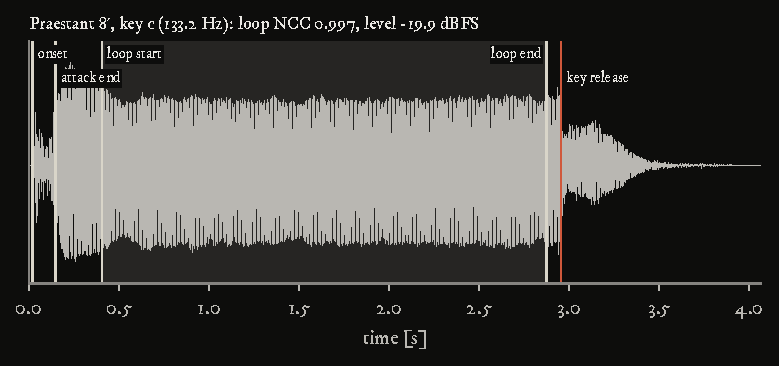
\includegraphics[width=\linewidth]{figs/pipe_anatomy.pdf}
\caption{Anatomy of one pipe sample (Praestant 8′, c). The engine plays the attack, loops the shaded
region while the key is held, and on release crossfades to just before the recorded key release so the
real release transient and decay follow.}
\label{fig:anatomy}
\end{figure}

\subsection{Clean-up}
After cutting, each pipe is cleaned moderately (this can be switched off with \code{--no-clean}):
\begin{itemize}
  \item a zero-phase high-pass at $0.55\times$ the pipe's fundamental (at least \SI{25}{Hz}) removes blower
        rumble below the pipe;
  \item a spectral noise reduction \citep{boll1979} with a noise print taken from the silent gaps of the same
        recording (over-subtraction 1.6, at most \SI{15}{dB} reduction, FFT size 2048) lowers the
        constant wind noise while keeping the pipe's own breath and chiff;
  \item the release tail ends where it reaches the remaining noise floor and is faded out over
        \SI{0.35}{s} instead of being cut.
\end{itemize}

\subsection{Noise layer}
Key clicks are detected as short events in the click recording and paired into key-down and key-up
events (174 click files in total, sorted into \code{down}, \code{up} and \code{other}). Fifteen stop-pull
sounds are cut from their recording. The blower noise between notes is collected from the stop
recordings (stretches of at least \SI{0.35}{s}, away from note tails) and joined with short crossfades
into seamless loops of about six seconds. These files are copied unchanged; the user may curate them
(the author removed clicks containing voice), and the folder \fn{noise/eigene} is reserved for the user's
own sounds and never touched by the script.

\subsection{Result}
\label{sec:measured}
All 287 pipes were found and assigned. Two pipes were flagged unusable -- Gedackt f (short sustain,
weak loop) and Gedackt f♯ (level unsteady by \SI{5}{dB}) -- and are replaced in the plug-in by the
neighbouring pipe, shifted to the exact meantone pitch. Figure~\ref{fig:tuning} shows the measured
pitch of every pipe of the non-compound stops. The flue stops lie within a few cents of quarter-comma
meantone at $a'=\SI{444.5}{Hz}$ (standard deviations 1.6--3.3\ct), which confirms both the temperament
and the reference pitch. The Trompete is on average \SI{13}{ct} sharp with a larger spread, as one would
expect from a reed that drifts with temperature and was tuned separately. The plug-in deliberately
keeps these deviations: they are part of the instrument. Figure~\ref{fig:levels} shows the level of every
pipe; the default stop volumes of the plug-in are set from the K-weighted loudness
\citep{itu1770} of all pipes of a stop, including their default distance, so that all stops start about
equally loud.

\begin{figure}[p]
\centering
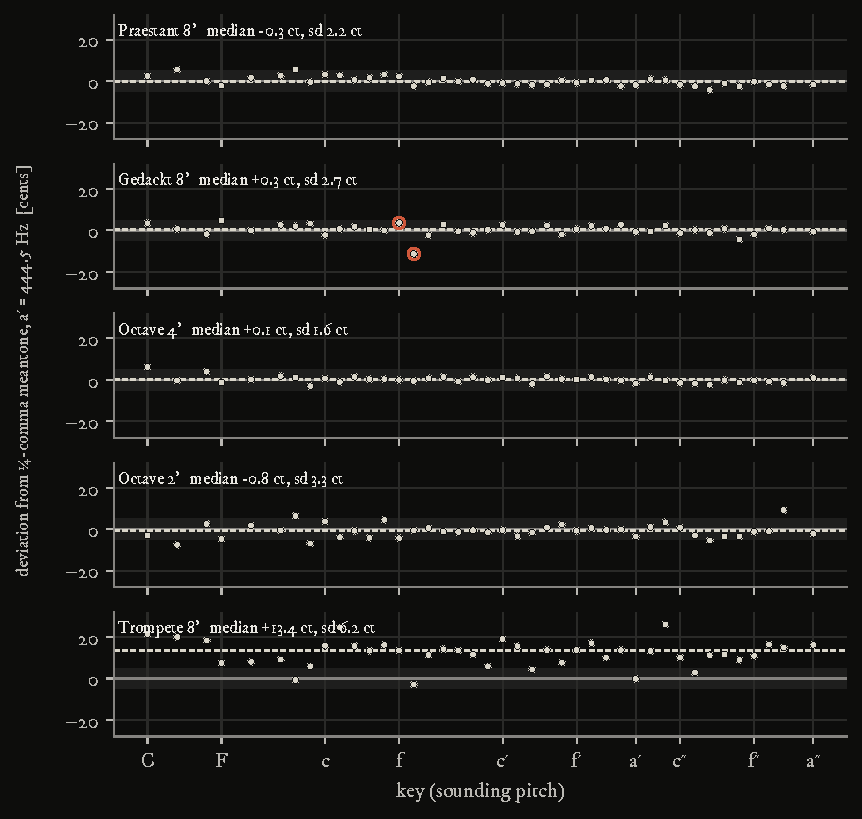
\includegraphics[width=\linewidth]{figs/tuning_measured.pdf}
\caption{Measured pitch of every pipe against quarter-comma meantone ($a'=\SI{444.5}{Hz}$). Grey band:
$\pm5$\ct; dashed line: median of the stop. Circled red: the two Gedackt pipes that were flagged
unusable and are replaced in the plug-in.}
\label{fig:tuning}
\end{figure}

\begin{figure}[h]
\centering
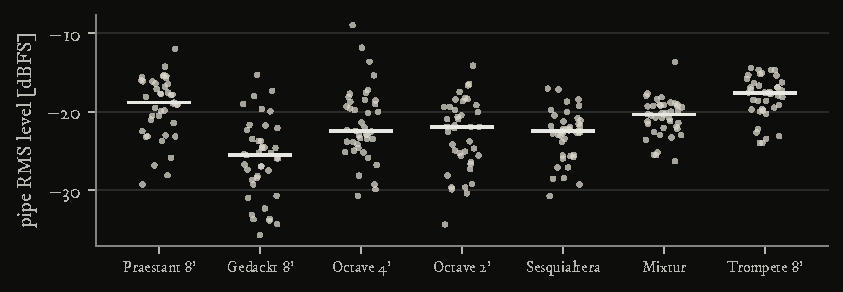
\includegraphics[width=\linewidth]{figs/levels.pdf}
\caption{RMS level of every pipe as recorded (no normalisation); bars mark the median per stop.}
\label{fig:levels}
\end{figure}

\subsection{The sample description}
\label{sec:sampledesc}
For every pipe \fn{rysum\_samples.json} stores, among others: key and file, \code{onset},
\code{attack\_end}, \code{loop\_start}, \code{loop\_end}, \code{loop\_ncc}, \code{release}, level,
nominal and measured frequency, deviation in cents, the mono method and alignment lag, the source
file and time, flags (\enquote{2 takes}, \enquote{weak loop}, \enquote{unsteady}, \dots) and the other
takes. The header records instrument, temperament, $a'$, the 41 keys with their physical index, and the
noise files.

% =====================================================================
\section{Plug-in architecture}
\label{sec:architecture}
% =====================================================================

\subsection{Framework and formats}
The plug-in is written in C++17 with JUCE~8.0.12 \citep{juce} and built with CMake as VST3 and
Standalone application (Windows, Visual Studio 2022; it also builds on Linux). A second build
configuration, \emph{Rysum Dev}, has its own plug-in ID so that a development version can be used next
to the stable one in the same host. Third-party code is limited to libmysofa \citep{libmysofa}
(BSD-3, reading SOFA HRTF files), the MTS-ESP client \citep{mtsesp} (0BSD) and the PFFFT FFT library
\citep{pffft}; zlib comes with JUCE.
The binary embeds fonts, the stop-knob and keyboard photographs, a grain texture, the FABIAN HRIR
set (\S\ref{sec:binaural}) and the weights of the \ui{Vox humana} (\fn{vox\_humana.nrv2}, \SI{3.4}{MB}, \S\ref{sec:vox}), whose engine is the
plug-in's own C++ code and needs no machine-learning library at run time. A third program, \emph{Rysum Konzert}, is built from the same sources: only
the 3D Saal and a line to join a player, for listeners (\S\ref{sec:konzert}).

\subsection{Source structure}
{\footnotesize
\begin{longtable}{@{}p{0.3\linewidth}p{0.64\linewidth}@{}}
\toprule
File & Responsibility \\
\midrule
\endhead
\fn{OrganEngine.*}     & voices, loops, releases, noise layer, encoding, degradation, room early reflections, FDN, effects \\
\fn{OrganLive.cpp}     & the living organ: bellows, pallets, walking listener, wear, pure tuning, Tonnetz walker (\S\ref{sec:live}) \\
\fn{OrganBodies.cpp}   & room motion: pipes as bodies in the Saal, the player's force, and the sound of the impacts (\S\ref{sec:roommotion}) \\
\fn{MeshAcoustics.h}   & a loaded room model for the sound: bounding-box tree, detour round edges, ray-traced reverb (\S\ref{sec:walk}) \\
\fn{SamplePitch.h}     & playback rate of a sample: native or corrected to the calibrated frequency (\S\ref{sec:tuning}) \\
\fn{Dsf*.h}            & reference tone: DSF oscillator, integrator, oversampling, renderer, MIDI-following instrument (\S\ref{sec:testton}) \\
\fn{SampleLibrary.*}   & reads the JSON and WAV files, substitutes unusable pipes \\
\fn{Spatial.h}         & AmbiX encoder, stereo panning, layouts, motion \\
\fn{Degrade.h}         & the \ui{Verfall} chain \\
\fn{WindChaos.h}       & the \ui{instabil} wind model \\
\fn{Modulation.h}      & LFOs, envelopes, routing definitions \\
\fn{Convolver.*}       & impulse-response room (stereo / AmbiX) with per-pipe rotation \\
\fn{PartConv.h}        & partitioned convolution (uniform and non-uniform), shared by all convolvers \\
\fn{FastFFT.h}         & wrapper around PFFFT, aligned buffers \\
\fn{Kernels.*}, \fn{KernelsAVX2.cpp}, \fn{KernelsImpl.inl} & SIMD kernels, compiled for SSE2 and AVX2/FMA, chosen at run time \\
\fn{RoomSim.h}, \fn{RoomTail.*} & simulated room: image sources, Eyring, ray tracer, synthesised tail, partitioned convolution \\
\fn{Binaural.*}        & HRIR sets, MagLS decoder design, binaural decoder \\
\fn{Transaural.h}      & crosstalk cancellation for two loudspeakers: filter design and real-time filter (\S\ref{sec:transaural}) \\
\fn{Walk3D.*}, \fn{WalkView.*} & the Saal in 3D: OBJ import, materials, software renderer, page \ui{Begehen} (\S\ref{sec:walk}) \\
\fn{WalkGpu.*}         & the same picture drawn by the graphics card (OpenGL 3.2 shader), with the processor as the way back (\S\ref{sec:walkgpu}) \\
\fn{WalkArrange.cpp}, \fn{WalkHands.cpp} & the player's hands in the 3D view: choosing and arranging pipes, layouts, undo, magnet, sweep; setting down, pinning, the bow, whirlwind, time, room size, lanterns, ears, the controls of the computer (\S\ref{sec:hands}) \\
\fn{RoomModels.*}      & the six built-in church rooms, generated as OBJ (\S\ref{sec:models}) \\
\fn{TimeDistance.h}    & \ui{Zeit als Entfernung}: a memory of up to \SI{20}{s} read further back the further forward one stands (\S\ref{sec:illusions}) \\
\fn{Audience.*}, \fn{QrCode.h} & \ui{Publikum}: the phone page on the local network, its HTTP server and the QR code (\S\ref{sec:audience}) \\
\fn{AudioWorkers.h}    & helper threads for the early reflections of the Saal (\S\ref{sec:perf}) \\
\fn{Lucier.*}        & Lucier mode: the response of $n$ passes through the room, built in the background \\
\fn{LucierPiece.*}   & Lucier's piece as a performance: recording, generations computed in the background, playback, WAV export \\
\fn{Speakers.*}      & loudspeaker layouts, IEM JSON files, AllRAD decoder and its real-time renderer \\
\fn{SpeakerView.*}   & the \ui{Lautsprecher} page: map, list, test signals \\
\fn{SpatialDegrade.h} & spatial degradation (\ui{Verfall $\cdot$ Raum}) and the parameters of the grain cloud \\
\fn{SpaceFx.h}        & double and long exposure of the sound field, the dispersive all-pass bank of the ice walls \\
\fn{Scala.h}           & Scala \code{.scl}/\code{.kbm} parser \\
\fn{MasterBus.h}       & \ui{Summe}: three-band EQ and compressor on the output (\S\ref{sec:summe}) \\
\fn{Automation.h}, \fn{ProcessorAutomation.cpp} & \ui{Verlauf}: lanes, points and segment shapes, the compiled curves the audio thread reads, the clocks, pieces and the six pieces that come with the plug-in (\S\ref{sec:verlauf}) \\
\fn{VerlaufView.*}     & the \ui{Verlauf} page: ruler, markers, lanes, tools, the plan of the spreading gestures \\
\fn{Concert.*}         & \ui{Konzert}: the link between a player and its listeners over TCP, jitter buffer, clocks, mirrored hands, figures and audio input (\S\ref{sec:konzert}) \\
\fn{ListenerApp.cpp}   & the program \emph{Rysum Konzert} for listeners \\
\fn{vox/*.h}, \fn{VoxStop.h} & the \ui{Vox humana}: C++ port of NeuralRysum v2 (pitch estimator, voice tracker, organ synth, timbre encoder, AVX2 kernels) and its glue to the engine (\S\ref{sec:vox}) \\
\fn{PluginProcessor.*} & parameters, state, patches, MIDI learn, sample loading, background builds \\
\fn{ProcessorScenes.cpp} & scenes (snapshots, morphing) and the dice (random settings) \\
\fn{PluginEditor.*}, \fn{*View.*}, \fn{Theme.h} & user interface \\
\fn{Tests/}            & offline render test, UI snapshot tool, benchmark (\fn{Bench.cpp}), dataset sampler (\fn{Dataset.cpp}, \S\ref{sec:dataset}), the \ui{Vox humana} against its PyTorch reference (\fn{VoxTest.cpp}) and through the whole plug-in (\fn{VoxRender.cpp}) \\
\bottomrule
\end{longtable}
}

\subsection{Threads and real-time safety}
The audio thread never allocates memory, reads files or waits for locks. Everything expensive happens
on the message thread or on background threads and is handed to the audio thread as an immutable
object behind a \code{std::shared\_ptr} that is swapped at the start of a block: the sample library,
an impulse response prepared for the current output format, the late reverb of the simulated room, the
binaural decoder filters. Data that the interface needs from the engine -- pipe positions, which pipes
sound, meters, LFO phases -- is exposed through atomics. Drawn motion paths are double-buffered so the
engine can read them without locking. What the player does in the 3D view (a shockwave, a throw, a knock, a formation, \S\ref{sec:hands})
travels the other way, as small commands in a lock-free single-producer queue (\fn{AbstractFifo}) that the audio thread empties at the start
of a block; targets and masks that are larger than a command (the places of a formation, the pipes a magnet acts on) are written into atomics
first and only announced by the command. The automation curves of the \ui{Verlauf} (\S\ref{sec:verlauf}) are compiled on the message thread into an
immutable table that the audio thread picks up like the other shared objects, and the network thread of the \ui{Konzert} (\S\ref{sec:konzert}) talks to
the audio thread through lock-free FIFOs only.

\subsection{Performance and CPU load}
\label{sec:perf}
Convolution dominates the cost of the plug-in: every pipe feeds up to $(N+1)^2$ Ambisonics channels
through a room of several seconds. The following measures keep this within real-time limits.

\paragraph{FFT.} All transforms use PFFFT \citep{pffft}, a SIMD FFT based on FFTPACK, wrapped in
\fn{RealFFT}. Spectra are kept in PFFFT's \emph{paired} layout (8 real and 8 imaginary values per
16 floats), which the complex multiply-accumulate kernels read directly, so no reordering is needed. All
buffers are 64-byte aligned (\fn{AlignedFloats}).

\paragraph{Partitioned convolution.} \fn{PartitionedConvolution} (\fn{PartConv.h}) is an overlap-save
convolver with a frequency-domain delay line. Its work is \emph{spread evenly over time}: the products
for the partitions of a stage are computed in small pieces in every host block, so there is no block
every $B$ samples that costs much more than the others. A stage has a \emph{lag} (1 or 2 blocks):
stages with lag 2 deliver their result one block later, which is accounted for in the partition
starts. All memory is allocated in \code{prepare()}; filter terms are swapped only at block boundaries,
which makes the crossfade between two responses (\S\ref{sec:room}) safe.

\paragraph{Non-uniform partitions.} A uniform partitioning with block 512 needs 282 partition products
per sample block for a 3\,s response; the layout used now needs 29 (7 + 6 + 16). The layouts are:
\begin{center}\small
\begin{tabularx}{\linewidth}{@{}llXl@{}}
\toprule
Use & Blocks (samples) & Stage starts / lags & Length \\
\midrule
IR room (\fn{Convolver})   & 512 / 2048 / 8192 & first 7 partitions of 512 ($\approx\SI{75}{ms}$), then 6 of 2048, then 8192 & file \\
\ui{Saal} tail (\fn{RoomTail}) & 256 / 2048 / 8192 & 256 / 4096 / 32768; lags 1/2/2 & $\le\SI{12}{s}$ \\
Binaural decoder           & 128 (one stage) & lag 1 & 36 ch $\to$ 2 \\
\bottomrule
\end{tabularx}
\end{center}

\paragraph{SIMD kernels.} The inner loops (complex multiply-accumulate, mixing of four channels, of
four-by-four channel blocks) are in \fn{KernelsImpl.inl}, which is compiled twice: for SSE2 (the
baseline) and for AVX2 with FMA. The table of function pointers (\fn{kern::Table}) is selected once at
start-up from \code{cpuid}; setting the environment variable \code{RYSUM\_NO\_AVX2} forces the SSE2 set.

\paragraph{Mixing and reflections.} Pipe signals are added to the Ambisonics bus four channels at a
time (\fn{mixGroup4}, \fn{mixInto}). Early reflections are rendered four taps at a time; taps are
sorted into high-order and first-order taps, and taps below $-\SI{90}{dB}$ are skipped. The AmbiX
encoder computes two sine/cosine pairs per pipe and obtains the remaining harmonics by recurrence.

\paragraph{Measurement.} The tool \fn{RysumBench} (CMake option \code{RYSUM\_BUILD\_BENCH}) renders
representative scenes block by block (128 samples, \SI{8}{s} each) and reports the render time per
block as a percentage of the time the block lasts. Table~\ref{tab:bench} gives the result on the
machine used for this paper, a shared 2-core Xeon (\SI{2.8}{GHz}) cloud VM. It is much slower than a
current desktop CPU and its timing is noisy, so only the order of magnitude should be read from it.
Repeated runs differ by several percent in the mean and by more in the worst block; the difference between
the AVX2 and SSE2 kernels was within this scatter, so \emph{no speed-up of AVX2 over SSE2 is claimed here}. No measurement of the previous
(JUCE FFT, uniform partitions) version exists either, so the gain from the optimisation is stated only
through the counts of partition products above and through the micro-benchmark below.
\begin{table}[t]
\centering\small
\begin{tabular}{@{}lrrr@{}}
\toprule
Scene (128-sample blocks) & mean & 99\,\% & 99.9\,\% \\
\midrule
stereo, dry                          &   7.8 &  15.1 &  19.0 \\
stereo, moving pipes, IR room        &  13.6 &  21.4 &  53.5 \\
3rd-order AmbiX, moving, IR room     &  21.0 &  34.5 &  51.2 \\
5th-order AmbiX, moving, IR room     &  21.6 &  36.9 &  61.4 \\
3rd-order binaural, IR room          &  22.2 &  42.1 &  56.5 \\
5th-order binaural, IR room          &  29.4 &  51.8 & 127.0 \\
3rd-order AmbiX, \ui{Saal}           &  54.9 &  99.8 & 157.5 \\
3rd-order AmbiX, \ui{Saal} + reflections & 111.9 & 186.9 & 291.3 \\
3rd-order binaural, \ui{Saal}        & 100.6 & 185.8 & 298.9 \\
5th-order AmbiX, effects, degradation & 29.2 &  52.2 & 102.7 \\
\bottomrule
\end{tabular}
\caption{Render time per block as a percentage of the block duration (AVX2 kernels, one run, 2-core cloud VM;
100\,\% is the real-time limit). Values above 100\,\% mean that the scene does not run in real time on this machine.}
\label{tab:bench}
\end{table}
On this VM the dense \ui{Saal} scenes and the reflection scene exceed real time, while all IR-room scenes
stay well below it on average; whether the \ui{Saal} scenes run on a given computer has to be tried there,
and the README lists the settings that reduce the load (lower Ambisonics order, fewer simulated pipes,
shorter room, reflections off).

A micro-benchmark of the convolver alone (one input, one output, host block 128, \SI{1}{s}/\SI{3}{s}/\SI{6}{s}
responses) gives a mean load of \SI{0.19}{\percent}/\SI{0.76}{\percent}/\SI{1.47}{\percent} for uniform
512-sample partitions and \SI{0.12}{\percent}/\SI{0.22}{\percent}/\SI{0.27}{\percent} for the non-uniform
512/2048/8192 layout; the worst block is of the same size in both cases (a 73.8\,\% outlier occurred once in
the 3\,s run and is attributed to the shared VM).

\paragraph{Several cores.} The table shows that the \ui{Saal} dominates, and within it the early reflections (every sounding pipe
its own 24 or 62 image sources). They are now rendered in twelve groups of sounds, each into its own bus, spread over helper threads
(\fn{AudioWorkers.h}: one pool per process, by default half the processor's cores and at most four). The audio thread never takes a
lock: it publishes the jobs, wakes the helpers, takes jobs itself and spins only for jobs a helper has already begun; while one instance
uses the pool, another does its jobs alone instead of waiting. The buses are summed in a fixed order, so the output is bit-identical whichever thread
rendered which group; the benchmark's WAV files of one and of three threads were compared sample by sample. On the author's desktop
(Ryzen~5 2600X, blocks of 128 samples) a scene with 48 reflected sounds and third-order reflections fell from 88\,\% to 45\,\% of the
audio thread's time and its worst block from 150\,\% to 68\,\%; a full 3D-view scene fell from 62\,\% to 42\,\%. \ui{Kerne für den Ton}
(\emph{automatisch}, 1--4) is a parameter: in a host that already fills every core, one can be the better choice. The helpers sleep while
fewer than eight sounds are reflected. Pipes flying in a shaped Saal (\S\ref{sec:roommotion}) keep a lower bound of their distance to the
nearest wall (less the way travelled since) and ask the walls again only when it may have run out; the walls and the listener's place are
worked out once per slice. This, too, is bit-identical and lowered the load of a drawn room with all pipes flying from 36--42\,\% to
29--35\,\%. \textbf{Ctrl+Shift+P} shows the audio load, the worst block, the cores and where the engine's time goes (before the pipes, the pipes,
the reflections, the late reverb). These figures are from a single machine and from the repository's README; they were not repeated for
this document.

\paragraph{Reflections that stay put.} Two later changes (15 November) halved the cost of the reflections once more. First, a pipe's image sources
were computed anew whenever anything in their key changed, compared exactly; since a pipe's resting place drifts by a few hundredths of a degree per
block, every reflected pipe was recomputed in every block, and with the Saal on the geometry alone took 23\,\% of the audio time. A pipe now counts as
moved only after a quarter of a degree or 0.5\,\% of its distance, the walking listener after a centimetre (a walk is about \SI{4}{mm} per block); the
delays still glide within the block, so level, high-frequency energy and the number of transients stay as before and only the fine timing of the
reflections differs. Second, a reflection whose delay does not change during a slice is now read from its delay line in one straight, vectorisable
pass instead of computing a ramped fractional position per sample, which had been more than half of the reflections' time; this path is bit-exact
against the general one (checked in place over a whole binaural Saal run). \fn{RysumBench} at 128 samples on the author's desktop, the old and new
builds alternating: the binaural third-order Saal fell from a mean of 46\,\% to 38\,\% with the first change (geometry 23\,\% $\rightarrow$ 2.7\,\%, worst
block from up to 386\,\% to 60\,\%) and from 69--70\,\% to 48--49\,\% with the second (measured separately, with one audio thread, so the two baselines differ);
the Saal with third-order reflections from 68--69\,\% to 48\,\%. With the graphics card drawing the 3D view, the depths used to aim at pipes and to hide
glows behind walls are still computed on the message thread; above 1000 triangles the helper threads share this work (\SI{4.4}{ms} $\rightarrow$
\SI{1.0}{ms} per frame with a model of 3600 triangles).

\subsection{Signal flow}
Figure~\ref{fig:signalflow} shows the signal path. The engine always renders into an internal
Ambisonics bus of the selected order (or a stereo pair), in slices of 64 samples
(\SI{1.3}{ms} at \SI{48}{kHz}): for every slice, pipe positions, modulation and spatial gains are
recomputed, and gains are ramped linearly across the slice. MIDI events split the slices so that notes
start sample-accurately. Up to 384 pipe voices and 48 noise voices can sound at once; when the pool is
full, the oldest releasing voice (else the oldest voice) is stolen.

The plug-in declares its output bus as fifth-order Ambisonics (36 channels). In \ui{Stereo},
\ui{Binaural} and \ui{Transaural} mode only channels 1/2 carry signal; in AmbiX mode the order 1--5 is selected in the
interface, and the interface warns when the host track has fewer channels than needed.

\begin{figure}[t]
\centering
\resizebox{\linewidth}{!}{%
\begin{tikzpicture}[
  box/.style={draw=ink2, line width=0.5pt, rounded corners=1.5pt, align=center, font=\footnotesize,
              minimum height=0.95cm, inner sep=3pt, text width=2.2cm},
  grp/.style={draw=muted, dashed, line width=0.4pt, rounded corners=3pt, inner sep=6pt},
  arr/.style={-{Stealth[length=1.8mm]}, line width=0.55pt, color=ink2},
  lab/.style={font=\scriptsize\itshape, text=muted}]
  \node[box, text width=1.7cm] (midi) at (0,0) {MIDI in\\ \scriptsize notes, CC, SysEx};
  \node[box] (keys) at (2.75,0) {Key logic\\ \scriptsize short octave, \ui{Halten}, sustain, tuning};
  \node[box] (mod)  at (6.2,3.5) {Modulation\\ \scriptsize 4 LFO, 2 env, 24 routes};
  \node[box] (play) at (6.2,1.75) {Sample player\\ \scriptsize Hermite, loop, release, \ui{Pfeife}, glitches};
  \node[box] (wind) at (6.2,0)    {Stop wind\\ \scriptsize pitch, level, tone, edge tones};
  \node[box] (vdeg) at (6.2,-1.75){\ui{Verfall}\\ \scriptsize per pipe};
  \node[box] (enc)  at (9.4,0)    {Encoder\\ \scriptsize AmbiX / stereo, distance, air, Doppler};
  \node[grp, fit=(play)(vdeg)(enc)] (vgrp) {};
  \node[lab, anchor=north west] at (vgrp.south west) {per pipe voice ($\le 384$)};
  \node[box] (noise) at (6.2,-4.2) {Noise layer \& effects\\ \scriptsize clicks, pulls, blower, FX};
  \node[box, text width=1.7cm, minimum height=3.6cm, fill=rubric!30!bg] (bus) at (12.5,0)
        {Bus\\[2pt] \scriptsize up to 36 ch\\ AmbiX (ACN/SN3D)\\ or stereo};
  \node[box, text width=1.9cm] (room) at (12.5,-4.2) {Room\\ \scriptsize IR convolver \emph{or} \ui{Saal} (\ui{Eis})};
  \node[box, text width=1.9cm] (sum) at (15.1,0) {\ui{Verfall} sum, master\\ \scriptsize exposures, sphere erosion};
  \node[box, text width=1.8cm] (out) at (17.7,0) {Output\\ \scriptsize Stereo, AmbiX 1--5, Binaural, Transaural; \ui{Summe}};
  \draw[arr] (midi) -- (keys);
  \draw[arr] (keys.east) -- (4.45,0) |- (play.west);
  \draw[arr] (keys.east) -- (4.45,0) |- (noise.west);
  \draw[arr] (play) -- (wind); \draw[arr] (wind) -- (vdeg);
  \draw[arr] (vdeg.east) -| (enc.south);
  \draw[arr] (mod.south) -- (play.north);
  \draw[arr] (mod.east) -| (enc.north);
  \draw[arr] (enc.east) -- (bus.west);
  \draw[arr] (noise.east) -- (8.6,-4.2) |- ($(enc.south west)!0.3!(enc.south east)+(0,-0.25)$) -- ($(enc.south west)!0.3!(enc.south east)$);
  \draw[arr] (enc.east) ++(0,-0.3) -- (10.95,-0.3) |- node[lab, pos=0.25, right] {sends} (room.west);
  \draw[arr] (room.north) -- (bus.south);
  \node[box, text width=1.9cm] (luc) at (15.1,-4.2) {Lucier\\ \scriptsize $n$ passes (optional)};
  \node[box, text width=1.9cm] (inp) at (6.2,-6.4) {Live input, \ui{Vox humana}\\ \scriptsize placed and moved with the pipes};
  \draw[arr] (bus) -- (sum); \draw[arr] (sum.south) -- (luc.north); \draw[arr] (luc.east) -| (out.south);
  \draw[arr] (inp.east) -- (10.2,-6.4) -- (10.2,-0.5);
\end{tikzpicture}}
\caption{Signal flow of the engine. Every pipe voice is processed and encoded on its own; modulation reaches
every stage. Room sends carry each pipe's direction (\S\ref{sec:ir}). The live input is encoded beside the pipes (\S\ref{sec:input}). The Lucier mode acts on the summed signal. On the whole field follow, in this order, the playback of
Lucier's piece, double and long exposure (\S\ref{sec:exposure}) and the spatial degradation (\S\ref{sec:spacedeg}); only then
is the field decoded for headphones, for two loudspeakers (\S\ref{sec:transaural}) or for a loudspeaker array. The living organ (\S\ref{sec:live}) acts
inside the voice stage (wind, pitch, wear) and on the pipe positions (the walking listener, the bodies of the room motion). After the decoding,
two illusions of the 3D view act on the output: \ui{Flüstern} adds the ear signals of pipes at the head, and \ui{Zeit als Entfernung} passes the whole
field and those ear signals through one memory, read as far back as the listener stands forward (\S\ref{sec:illusions}). The neural \ui{Vox humana}
is encoded beside the pipes in the same way as the live input (\S\ref{sec:vox}). The very last step of every output is the \ui{Summe}, an equaliser and
a compressor (\S\ref{sec:summe}); the curves of the \ui{Verlauf} (\S\ref{sec:verlauf}) set the controls of every stage before modulation is added.}
\label{fig:signalflow}
\end{figure}

\subsection{Parameters, state and patches}
All sound-relevant settings are host parameters (automatable, MIDI-learnable) held in a JUCE
\code{AudioProcessorValueTreeState}. New parameters are only ever appended and list-type parameters
only gain entries at the end, because projects and patches store indices. Patches are plain XML files
with the extension \fn{.rysum} in \fn{Documents/Rysum/Patches}. A patch contains everything that makes
the sound -- stops, all sliders, pipe layouts and positions, muted pipes, modulation routings, drawn
paths, Scala files and the path of a loaded impulse response -- but not the output format, the headphone
settings or the samples folder, which belong to the session. A factory set (version~17, 175 patches,
Appendix~\ref{app:patches}) is written on first start; deleted factory patches stay deleted until a
newer set is shipped. The room model of the 3D view belongs to the project, not to patches, with one exception: a patch saved
while one of the six built-in rooms is loaded remembers that room and whether the light is off, and loading it loads the room
again, fits the Saal to it and puts the listener at its listening place (\S\ref{sec:models}). The lanes of the \ui{Verlauf} also belong to the project,
not to patches, so that loading a patch in the middle of a piece keeps the piece going; a piece can be kept as a file of its own
(\fn{Documents/Rysum/Stücke/*.rysumstueck}, \S\ref{sec:verlauf}). Parameters that were added later (the \ui{Summe}, the effects per stop, the
\ui{Vox humana}) were appended at the end, so older projects keep their indices and open with these switched off. \ui{Alles zurücksetzen \dots} in
the patch menu returns, after a confirmation, to the state of a new instance: every parameter, the room, the 3D model and where one stands in it,
the lanterns, the layouts and the patch name; in the 3D view nothing stays chosen, pinned or paused and every pipe flies home. Only the samples
folder is kept.

\subsection{A dataset for neural synthesis}
\label{sec:dataset}
A further tool, \fn{RysumDataset} (\fn{tests/Dataset.cpp}, run by \fn{scripts/make\_dataset.ps1}), lets the plug-in sample itself into a dataset
for training a neural synthesis network. The plug-in plays by itself, faster than real time, and every clip is written with its notes and settings:
the audio (by default 10-second clips, stereo, \SI{48}{kHz}, 16-bit WAV), a MIDI file of its notes, and one line of \fn{metadata.jsonl} per clip
(training or validation, kind, stops, every note with its times and velocity, levels, and the parameters that differ from a freshly opened plug-in),
together with \fn{dataset.json}, which lists every parameter with its default and range. 40\,\% of the clips are single pipes (one stop, one held note),
40\,\% registrations of one to five stops playing a phrase (lines, chords, a line over a held chord, free notes) and 20\,\% factory patches playing a
phrase. Every parameter is reset before each clip, keys that are assigned as MIDI buttons are left out, and the tool waits for the reverb of the Saal
to be built. The same seed gives the same notes and settings (the organ's own chance means two runs are not identical sample for sample); clips
that would clip are turned down and the amount is recorded, a silent draw is repeated, and a stopped run carries on where it was. The illusions of the
3D view are not part of it. Ten hours are 3600 clips, about \SI{7}{GB}, at roughly 20--25 times real time.
Such a dataset has since been rendered: 3600 clips of \SI{10}{s} (1439 single pipes, 1441 registrations, 720 patches). Its pipes and registrations
(2880 clips, 2736 of them for training, \SI{7.6}{h}) trained the network that is now the \ui{Vox humana} (\S\ref{sec:vox}); the patch clips were left
out, because their effects are not part of the instrument \citep{neuralrysum2}.

% =====================================================================
\section{Sound generation}
\label{sec:voice}
% =====================================================================

\subsection{Sample playback}
A voice reads its pipe's mono sample with four-point cubic Hermite interpolation at a rate
\begin{equation}
  r = r_0 \cdot 2^{\Delta c/1200}\cdot D,
\end{equation}
where $r_0$ converts the file rate (\SI{48}{kHz}) to the host rate and contains the static tuning shift,
$\Delta c$ the sum of all time-varying pitch offsets in cents (stop wind, wind wobble, global wind
gusts, tremulant, modulation) and $D$ the Doppler factor (\S\ref{sec:distance}). When the read
position approaches the loop end it crossfades linearly into the corresponding position one loop length earlier
(crossfade up to \SI{30}{ms}, at most a third of the loop); the loop points were chosen for high correlation,
so a linear fade suffices. On key release the voice crossfades within \SI{40}{ms} from
wherever it is to \SI{40}{ms} before the recorded release point and then plays the recorded release,
so every note ends with the real sound of that pipe's pallet closing.

The \emph{Praestant 16′} reads the Praestant 8′ samples at half speed; every key of the virtual
16′ uses the 8′ pipe of the same name. Notes held by the sustain pedal (CC64) or by \ui{Halten}
(\S\ref{sec:control}) behave exactly like held keys.

\subsection{Action and wind noise}
\paragraph{Key clicks.} On every key-down a click is chosen from the \code{down} pool (never the same as
last time) and played, on key-up one from the \code{up} pool. MIDI velocity $v\in[0,1]$ controls level
and brightness of the click, also on release:
\begin{equation}
  g_\text{click}(v) = 0.04 + 0.96\,v^{1.5},\qquad
  f_c(v) = \SI{900}{Hz}\cdot\left(\tfrac{20000}{900}\right)^{\min(1,\,1.25 v)} ,
\end{equation}
where $f_c$ is the corner of a one-pole low-pass. The clicks come from the console position; the
parameter \ui{Klick $\rightarrow$ ins Anschlagen} blends them towards the mean position of the
sounding pipes, so that part of the click appears inside the attack of the pipes, where in reality
the pallet noise is heard through the pipe foot. The pools hold the clicks of both sessions (\S\ref{sec:recording}).

\paragraph{Key-click resonance.} With \ui{Klick-Resonanz} (tab \ui{Resonanz} in the \ui{Traktur} section) every key
click also excites a bank of up to six two-pole resonators tuned to the harmonics $hf_0$ ($h=1\dots6$, below
$0.45f_s$) of the pressed key in the tuning in use. Harmonic $h$ decays with time constant
$\tau_h=\tau/\sqrt h$ (\ui{Nachklang} $\tau$, \SIrange{0.02}{4}{s}), so the upper ones die sooner; its gain is
normalised by the resonator's peak gain $\propto 1/(1-r)$ and tilted by $h^{-1.6(1-b)}$ with \ui{Helligkeit} $b$.
The amount grows with velocity ($0.6+0.4v$). The result is a short, bell-like tone at the console with the
pitch of the key: the action seems to sing.

\paragraph{Stop pulls.} Pulling or pushing a stop plays one of the recorded stop-knob sounds.

\paragraph{Blower.} \ui{Wind (global)} plays the blower loop (since the second session the clean \SI{3.7}{s} loop of
\S\ref{sec:recording}). In Ambisonics it is encoded
omnidirectionally; with \ui{Gebläse ringsum} (Effects page) four uncorrelated parts of the recording are
placed in a tetrahedron so that the blower surrounds the listener. Above about 35\,\%, \ui{Wind
(global)} also makes the wind supply unstable: a shared gust signal (one value per 16 samples, the same
for all pipes, since they share a wind chest) modulates pitch and level of every pipe, increasingly
wildly towards 100\,\%.

\paragraph{Tremulant.} A tremulant periodically interrupts the wind. It is modelled as a slightly
asymmetric wave shared by all pipes that modulates pitch and level, with a small amount of added wind
noise; rate and depth are parameters (CC1 controls the depth).

\subsection{The pipe's own sound (\ui{Pfeife})}
\label{sec:pipesound}
A fourth tab on the \ui{Raum} page (next to \ui{Bewegung}, \ui{Hall} and \ui{Wolke}) shapes the sound of the pipes of a
stop (\fn{PipeSoundParams}). Everything is neutral by default, and every control is also a per-pipe modulation target
(\S\ref{sec:modulation}).

\paragraph{Ansprache (attack).} The preprocessing stores for every pipe the onset and the end of its measured
attack (\code{attack\_end}, \S\ref{sec:sampledesc}). Between the two an envelope $e$ falls from 1 to 0 as a raised cosine. \ui{Ansprache}
$g\in[-1,1]$ multiplies the signal by $(1+3g^+e)(1-g^-e)$: positive values lift the chiff by up to
\SI{+12}{dB}, negative ones let the pipe swell in softly; the sustained tone is unchanged. \ui{Schärfe} $s$ adds
$3se\,(x-\mathrm{LP}_{\SI{2.5}{kHz}}(x))$, the highs of the attack (a hissing chiff). \ui{Nur Ansprache} $q$ scales the
signal by $1-q(1-e)$, so at 100\,\% only the chiff is left. \ui{Ansprache wiederholen} plays the attack again as a
short burst, up to six times, each repeat $0.82$ times as loud as the one before (decided when the note starts).

\paragraph{Abriss (release).} When the key is let go and the pallet closes, a puff of air sounds at the pipe:
noise through a two-pole band-pass at $f_c=k_s f_0$ (clamped to \SIrange{250}{12000}{Hz}, with $k_s$ from 2.5 for
the Gedackt to 8 for the Mixtur), decaying with $\tau=\mathrm{clamp}(0.04\sqrt{130/f_0},\,0.008,\,0.09)$\,s, as
loud as the key was struck and scaled by the pipe's level.

\paragraph{Upper partials as a layer.} Above \ui{Obertöne ab} (default \SI{4}{kHz}) a second-order Butterworth
high-pass (state-variable form) splits off the upper partials $h$; the output is $x+(G\,t-1)h$ with the layer
gain $G$ (\ui{Obertöne Pegel}, $\pm\SI{24}{dB}$) and a transient shaper
$t=\mathrm{clamp}\bigl((E_f/E_s)^{1.5\sigma},0.2,5\bigr)$ from a fast (0.7/\SI{6}{ms}) and a slow (25/\SI{120}{ms})
envelope follower, $\sigma$ = \ui{Obertöne Anschlag}: positive values make the attack of the upper layer spiky,
negative ones leave only its surface. Mixtur and Sesquialtera can glitter on their own without making the whole
sound brighter.

\emph{Status:} the key-click resonance, the \ui{Pfeife} tab and the glitches below were added after the verification run of
1~November and are described from the source code. The render test of 15~November (\S\ref{sec:verification}) covers them: \ui{Ansprache},
\ui{Schärfe}, \ui{Nur Ansprache}, \ui{Wiederholen}, \ui{Abriss}, the upper partials, \ui{Luft umkehren}, the key-click resonance (its tail at the
key's pitch \SI{31}{dB} above a semitone up) and the four glitches each change the sound as described, and every per-pipe modulation target of
the tab gives exactly the same result as the same setting made by hand.

\subsection{Stop wind: the classic model}
\label{sec:stopwind}
Every stop has a \ui{Wind} slider: how far the stop is drawn, from 0 (closed, silent) to 1 (fully
drawn). On a real organ a half-drawn slider starves the pipes: they get quieter, flatter, duller and
unsteady. With $w$ the smoothed stop wind and $\ell=1-w$ the lack of wind, the engine applies (every
16 samples)
\begin{align}
  \Delta c_\text{wind} &= -75\,\ell^{3/2} + 35\,\ell^{2}\, b(t)\ \ \text{ct}, \\
  a_\text{wind} &= w^{1.6}\,\bigl(1 + 0.4\,\ell\, b(t)\bigr), \\
  f_{c,\text{wind}} &= 250 + 16000\,w^2\ \ \text{Hz},
\end{align}
where $b(t)$ is a slow \enquote{breathing} sum of three sines with random rates that runs faster the
less wind there is, and $f_{c,\text{wind}}$ the corner of a one-pole low-pass. At full wind ($w>0.995$)
the filter is bypassed. Figure~\ref{fig:stopwind} plots the static part of these curves.

\begin{figure}[h]
\centering
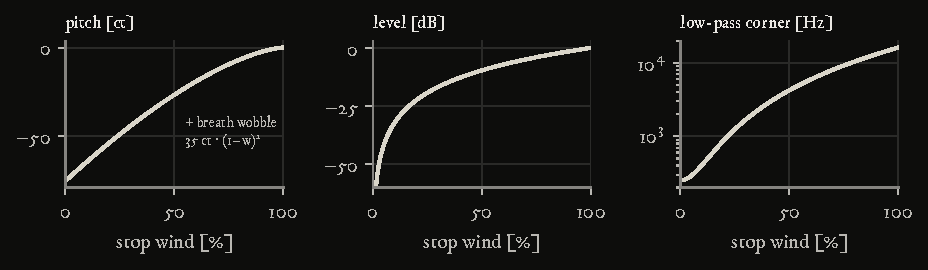
\includegraphics[width=\linewidth]{figs/stopwind.pdf}
\caption{Classic stop-wind model: pitch drop, level and tone of a starving pipe as functions of the
stop wind.}
\label{fig:stopwind}
\end{figure}

\subsection{Stop wind: the unstable model}
\label{sec:windchaos}
The second wind model (\ui{Registerwind: instabil}, \fn{WindChaos.h}) adds what a starving
\emph{flue} pipe does besides getting quieter and flatter. When the pressure at the pipe foot drops, the
air jet leaving the flue becomes slow. Next to the pipe tone an \emph{edge tone} becomes audible: the
jet oscillating against the upper lip at a frequency set by the jet velocity, which is proportional to
the square root of the pressure \citep{fletcher1998,fabre2012}. The model was designed around
four observations that the user formulated from listening to the real organ: the whistle is steady as
long as the wind is steady; it falls in pitch and gets quieter as the wind falls; it is different for
every pipe; and it is always the same for the same pipe.

Every pipe receives one or two edge tones (\emph{mouth tones}) with fixed, pseudo-random properties derived only from stop
and key. The tone belongs to the pipe: it appears a few partials above the pipe's own note and comes down towards it as the
wind falls. Its starting frequency is
\begin{equation}
  f_\text{top} = f_0\,r\,\Bigl(\frac{\SI{262}{Hz}}{f_0}\Bigr)^{0.35},\qquad r\in[2.3,\,6]\ \text{(log-uniform)},
\end{equation}
limited to $[\max(\SI{180}{Hz},1.3f_0),\ \min(\SI{9}{kHz},0.4f_s)]$ (large pipes have relatively small mouths, so their tone sits
further up; small pipes' nearer to the note). The other properties are the wind $w_\text{on}\in[0.30,0.55]$ below which
it appears, its level, how narrow its breath is ($q\in[10,32]$), how much clean tone is in it (20--50\,\%) and a
\enquote{lock} $\lambda$ that describes how strongly it is pulled to the pipe's
resonances. A second, weaker tone ($1.35$--$1.85$ times higher, appearing at $0.8\,w_\text{on}$) exists on about 45\,\% of the pipes.
(Until 14 November the tone was a clean whistle between \SIrange{2.2}{7}{kHz}, independent of the note.) At stop wind
$w<w_\text{on}$ the free edge tone is
\begin{equation}
  f_\text{free}(w) = f_\text{top}\sqrt{w/w_\text{on}} .
\end{equation}
It leans towards the nearest resonance of the pipe, $f_k = f_0\,k\,(1+0.0025(k-1))$ (only odd $k$ for a
stopped Gedackt), in the logarithmic domain,
\begin{equation}
  \ln f = \ln f_\text{free} + \lambda\,\bigl(\ln f_k - \ln f_\text{free}\bigr),
\end{equation}
with hysteresis: the resonance index $k$ only changes when $f_\text{free}$ is more than
$(0.5+0.3\lambda)$ resonance spacings away. Hence a strongly locked pipe moves in small hops instead of
gliding (Figure~\ref{fig:edgetone}). The level follows
\begin{equation}
  A(w) = A_0\cdot\min\!\Bigl(1,\tfrac{1-x}{0.12}\Bigr)\,x^{1.3},\qquad x = w/w_\text{on},
\end{equation}
a soft onset below $w_\text{on}$, then fading as the jet weakens.

A slow jet is turbulent, so the mouth tone is not a clean whistle. Most of it is \emph{breath}, noise through a band-pass of
quality $q$ around its frequency (brought to the level a tone of amplitude~1 would have), with only a core of tone in it: a rotating
phasor $\sin\phi$ with a little of its octave, $\sin\phi+\tfrac12\sin\phi\cos\phi$, weighted by the pipe's share of tone. Both flutter
all the time. Two noises, smoothed over \SI{0.30}{s} ($n_s$) and over \SI{22}{ms} ($n_q$) and each brought to unit variance, set the pitch
and a third quick one ($n_g$) the loudness:
\begin{gather}
  \Delta c = u\,(16\,n_s + 7\,n_q)\ \text{ct},\qquad
  g = \operatorname{clip}_{[0.15,\,2.2]}\bigl(1 + u\,(0.3\,n_g + 0.25\,n_s)\bigr),\\
  u = \bigl(0.6+0.9\,(1-x)\bigr)(1-0.5\lambda),
\end{gather}
so the weaker the wind, the more it wavers, and a tone that sits on a resonance wavers less. In addition the pipe itself breathes:
noise through a wide band-pass ($Q=0.9$) at $5f_0$ (limited to \SIrange{0.7}{5}{kHz}), what the pipe's body lets through, with the level
$0.18\,h^2$, $h=\operatorname{clip}_{[0,1]}\bigl((0.5-w)/0.4\bigr)$, swelling and sinking by up to 35\,\% with the slow noise (it replaces the
white hiss of the first version). Below roughly 15\,\% wind the speech sputters: the pipe tone drops out for a few milliseconds at a
time. The reed (Trompete) chatters instead of whistling; its mouth tone and breath are halved. At full wind none of this is active, so the
classic and the unstable model are bit-identical there and patches sound the same in both. The pallet of the living organ
(\ui{Ventil}, \S\ref{sec:live}) lets these sounds in only in the unstable model.

\begin{figure}[h]
\centering
\resizebox{\linewidth}{!}{% generated by make_edgetone_tikz.pl - do not edit
\begin{tikzpicture}[font=\footnotesize, x=1cm, y=1cm]
\draw[muted, line width=0.4pt] (0,0) rectangle (8.2,3.4);
\draw[muted!60, dotted, line width=0.4pt] (0,0.742) -- (8.2,0.742) node[right, text=muted, font=\scriptsize] {1$f_0$};
\draw[muted!60, dotted, line width=0.4pt] (0,1.488) -- (8.2,1.488) node[right, text=muted, font=\scriptsize] {2$f_0$};
\draw[muted!60, dotted, line width=0.4pt] (0,2.238) -- (8.2,2.238) node[right, text=muted, font=\scriptsize] {3$f_0$};
\draw[muted!60, dotted, line width=0.4pt] (0,2.992) -- (8.2,2.992) node[right, text=muted, font=\scriptsize] {4$f_0$};
\draw[muted] (0,0.000) -- (-0.08,0.000) node[left, text=ink2] {0};
\draw[muted] (0,0.850) -- (-0.08,0.850) node[left, text=ink2] {300};
\draw[muted] (0,1.700) -- (-0.08,1.700) node[left, text=ink2] {600};
\draw[muted] (0,2.550) -- (-0.08,2.550) node[left, text=ink2] {900};
\draw[muted] (0,3.400) -- (-0.08,3.400) node[left, text=ink2] {1200};
\draw[muted] (1.118,0) -- (1.118,-0.08) node[below, text=ink2] {40};
\draw[muted] (2.982,0) -- (2.982,-0.08) node[below, text=ink2] {30};
\draw[muted] (4.845,0) -- (4.845,-0.08) node[below, text=ink2] {20};
\draw[muted] (6.709,0) -- (6.709,-0.08) node[below, text=ink2] {10};
\node[text=ink2, rotate=90] at (-1.0,1.70) {mouth-tone frequency [Hz]};
\node[text=ink2] at (4.10,-0.75) {stop wind [\%]  (falling \(\rightarrow\))};
\draw[muted, line width=1.0pt, line join=round] (0.186,2.970) -- (0.239,2.964) -- (0.291,2.956) -- (0.343,2.947) -- (0.395,2.938) -- (0.448,2.929) -- (0.500,2.920) -- (0.552,2.911) -- (0.604,2.902) -- (0.657,2.893) -- (0.709,2.884) -- (0.761,2.875) -- (0.813,2.866) -- (0.865,2.856) -- (0.918,2.847) -- (0.970,2.838) -- (1.022,2.829) -- (1.074,2.820) -- (1.127,2.810) -- (1.179,2.801) -- (1.231,2.791) -- (1.283,2.782) -- (1.336,2.773) -- (1.388,2.763) -- (1.440,2.753) -- (1.492,2.744) -- (1.545,2.734) -- (1.597,2.725) -- (1.649,2.715) -- (1.701,2.705) -- (1.754,2.695) -- (1.806,2.686) -- (1.858,2.676) -- (1.910,2.666) -- (1.963,2.656) -- (2.015,2.646) -- (2.067,2.636) -- (2.119,2.626) -- (2.171,2.589) -- (2.224,2.569) -- (2.276,2.558) -- (2.328,2.548) -- (2.380,2.538) -- (2.433,2.528) -- (2.485,2.518) -- (2.537,2.507) -- (2.589,2.497) -- (2.642,2.487) -- (2.694,2.476) -- (2.746,2.466) -- (2.798,2.455) -- (2.851,2.445) -- (2.903,2.434) -- (2.955,2.424) -- (3.007,2.413) -- (3.060,2.402) -- (3.112,2.391) -- (3.164,2.380) -- (3.216,2.370) -- (3.269,2.359) -- (3.321,2.348) -- (3.373,2.336) -- (3.425,2.325) -- (3.477,2.314) -- (3.530,2.303) -- (3.582,2.291) -- (3.634,2.280) -- (3.686,2.269) -- (3.739,2.257) -- (3.791,2.246) -- (3.843,2.234) -- (3.895,2.222) -- (3.948,2.210) -- (4.000,2.199) -- (4.052,2.187) -- (4.104,2.175) -- (4.157,2.163) -- (4.209,2.150) -- (4.261,2.138) -- (4.313,2.126) -- (4.366,2.114) -- (4.418,2.101) -- (4.470,2.089) -- (4.522,2.076) -- (4.575,2.063) -- (4.627,2.050) -- (4.679,2.038) -- (4.731,2.025) -- (4.783,2.011) -- (4.836,1.998) -- (4.888,1.985) -- (4.940,1.972) -- (4.992,1.958) -- (5.045,1.945) -- (5.097,1.931) -- (5.149,1.917) -- (5.201,1.903) -- (5.254,1.889) -- (5.306,1.853) -- (5.358,1.825) -- (5.410,1.809) -- (5.463,1.795) -- (5.515,1.781) -- (5.567,1.766) -- (5.619,1.752) -- (5.672,1.737) -- (5.724,1.722) -- (5.776,1.707) -- (5.828,1.692) -- (5.881,1.677) -- (5.933,1.661) -- (5.985,1.646) -- (6.037,1.630) -- (6.089,1.614) -- (6.142,1.598) -- (6.194,1.582) -- (6.246,1.565) -- (6.298,1.549) -- (6.351,1.532) -- (6.403,1.515) -- (6.455,1.497) -- (6.507,1.480) -- (6.560,1.462) -- (6.612,1.444) -- (6.664,1.426) -- (6.716,1.407) -- (6.769,1.388) -- (6.821,1.369) -- (6.873,1.350) -- (6.925,1.330) -- (6.978,1.310) -- (7.030,1.290) -- (7.082,1.269) -- (7.134,1.248) -- (7.187,1.227) -- (7.239,1.205) -- (7.291,1.182) -- (7.343,1.159) -- (7.395,1.136) -- (7.448,1.079) -- (7.500,1.051) -- (7.552,1.026) -- (7.604,1.001) -- (7.657,0.976) -- (7.709,0.949) -- (7.761,0.922) -- (7.813,0.894) -- (7.866,0.865) -- (7.918,0.835) -- (7.970,0.803);
\draw[muted, line width=1.0pt] (4.90,3.15) -- (5.30,3.15) node[right, text=ink2, font=\scriptsize] {free (lock 0.05)};
\draw[s1, line width=1.0pt, line join=round] (0.186,2.988) -- (0.239,2.987) -- (0.291,2.986) -- (0.343,2.984) -- (0.395,2.983) -- (0.448,2.982) -- (0.500,2.980) -- (0.552,2.979) -- (0.604,2.977) -- (0.657,2.976) -- (0.709,2.974) -- (0.761,2.973) -- (0.813,2.971) -- (0.865,2.970) -- (0.918,2.968) -- (0.970,2.967) -- (1.022,2.965) -- (1.074,2.964) -- (1.127,2.962) -- (1.179,2.961) -- (1.231,2.959) -- (1.283,2.957) -- (1.336,2.956) -- (1.388,2.954) -- (1.440,2.953) -- (1.492,2.951) -- (1.545,2.949) -- (1.597,2.948) -- (1.649,2.946) -- (1.701,2.944) -- (1.754,2.943) -- (1.806,2.941) -- (1.858,2.939) -- (1.910,2.938) -- (1.963,2.936) -- (2.015,2.934) -- (2.067,2.932) -- (2.119,2.931) -- (2.171,2.929) -- (2.224,2.927) -- (2.276,2.925) -- (2.328,2.923) -- (2.380,2.922) -- (2.433,2.920) -- (2.485,2.918) -- (2.537,2.916) -- (2.589,2.914) -- (2.642,2.912) -- (2.694,2.910) -- (2.746,2.908) -- (2.798,2.906) -- (2.851,2.904) -- (2.903,2.902) -- (2.955,2.679) -- (3.007,2.296) -- (3.060,2.266) -- (3.112,2.262) -- (3.164,2.260) -- (3.216,2.258) -- (3.269,2.257) -- (3.321,2.255) -- (3.373,2.253) -- (3.425,2.252) -- (3.477,2.250) -- (3.530,2.248) -- (3.582,2.246) -- (3.634,2.245) -- (3.686,2.243) -- (3.739,2.241) -- (3.791,2.239) -- (3.843,2.237) -- (3.895,2.236) -- (3.948,2.234) -- (4.000,2.232) -- (4.052,2.230) -- (4.104,2.228) -- (4.157,2.226) -- (4.209,2.224) -- (4.261,2.222) -- (4.313,2.220) -- (4.366,2.218) -- (4.418,2.216) -- (4.470,2.214) -- (4.522,2.212) -- (4.575,2.210) -- (4.627,2.207) -- (4.679,2.205) -- (4.731,2.203) -- (4.783,2.201) -- (4.836,2.198) -- (4.888,2.196) -- (4.940,2.194) -- (4.992,2.191) -- (5.045,2.189) -- (5.097,2.187) -- (5.149,2.184) -- (5.201,2.182) -- (5.254,2.179) -- (5.306,2.176) -- (5.358,2.174) -- (5.410,2.171) -- (5.463,2.169) -- (5.515,2.166) -- (5.567,2.163) -- (5.619,2.160) -- (5.672,2.157) -- (5.724,2.154) -- (5.776,2.151) -- (5.828,2.148) -- (5.881,2.145) -- (5.933,1.587) -- (5.985,1.518) -- (6.037,1.510) -- (6.089,1.508) -- (6.142,1.505) -- (6.194,1.503) -- (6.246,1.500) -- (6.298,1.498) -- (6.351,1.495) -- (6.403,1.492) -- (6.455,1.490) -- (6.507,1.487) -- (6.560,1.484) -- (6.612,1.481) -- (6.664,1.478) -- (6.716,1.475) -- (6.769,1.472) -- (6.821,1.469) -- (6.873,1.466) -- (6.925,1.462) -- (6.978,1.459) -- (7.030,1.455) -- (7.082,1.451) -- (7.134,1.448) -- (7.187,1.444) -- (7.239,1.440) -- (7.291,1.435) -- (7.343,1.431) -- (7.395,1.426) -- (7.448,1.421) -- (7.500,1.416) -- (7.552,1.411) -- (7.604,1.406) -- (7.657,1.400) -- (7.709,1.394) -- (7.761,1.171) -- (7.813,0.795) -- (7.866,0.763) -- (7.918,0.756) -- (7.970,0.752);
\draw[s1, line width=1.0pt] (4.90,2.83) -- (5.30,2.83) node[right, text=ink2, font=\scriptsize] {open pipe, lock 0.85};
\draw[rysred, line width=1.0pt, line join=round] (0.186,2.335) -- (0.239,2.334) -- (0.291,2.333) -- (0.343,2.332) -- (0.395,2.331) -- (0.448,2.330) -- (0.500,2.329) -- (0.552,2.328) -- (0.604,2.327) -- (0.657,2.325) -- (0.709,2.324) -- (0.761,2.323) -- (0.813,2.322) -- (0.865,2.321) -- (0.918,2.320) -- (0.970,2.318) -- (1.022,2.317) -- (1.074,2.316) -- (1.127,2.315) -- (1.179,2.314) -- (1.231,2.312) -- (1.283,2.311) -- (1.336,2.310) -- (1.388,2.309) -- (1.440,2.307) -- (1.492,2.306) -- (1.545,2.305) -- (1.597,2.303) -- (1.649,2.302) -- (1.701,2.301) -- (1.754,2.300) -- (1.806,2.298) -- (1.858,2.297) -- (1.910,2.296) -- (1.963,2.294) -- (2.015,2.293) -- (2.067,2.291) -- (2.119,2.290) -- (2.171,2.289) -- (2.224,2.287) -- (2.276,2.286) -- (2.328,2.284) -- (2.380,2.283) -- (2.433,2.282) -- (2.485,2.280) -- (2.537,2.279) -- (2.589,2.277) -- (2.642,2.276) -- (2.694,2.274) -- (2.746,2.273) -- (2.798,2.271) -- (2.851,2.270) -- (2.903,2.268) -- (2.955,2.266) -- (3.007,2.265) -- (3.060,2.263) -- (3.112,2.262) -- (3.164,2.260) -- (3.216,2.258) -- (3.269,2.257) -- (3.321,2.255) -- (3.373,2.253) -- (3.425,2.252) -- (3.477,2.250) -- (3.530,2.248) -- (3.582,2.246) -- (3.634,2.245) -- (3.686,2.243) -- (3.739,2.241) -- (3.791,2.239) -- (3.843,2.237) -- (3.895,2.236) -- (3.948,2.234) -- (4.000,2.232) -- (4.052,2.230) -- (4.104,2.228) -- (4.157,2.226) -- (4.209,2.224) -- (4.261,2.222) -- (4.313,2.220) -- (4.366,2.218) -- (4.418,2.216) -- (4.470,2.214) -- (4.522,2.212) -- (4.575,2.210) -- (4.627,2.207) -- (4.679,2.205) -- (4.731,2.203) -- (4.783,2.201) -- (4.836,2.198) -- (4.888,2.196) -- (4.940,2.194) -- (4.992,2.191) -- (5.045,2.189) -- (5.097,2.187) -- (5.149,2.184) -- (5.201,2.182) -- (5.254,2.179) -- (5.306,2.176) -- (5.358,2.174) -- (5.410,2.171) -- (5.463,2.169) -- (5.515,2.166) -- (5.567,2.163) -- (5.619,2.160) -- (5.672,2.157) -- (5.724,2.154) -- (5.776,2.151) -- (5.828,2.148) -- (5.881,2.145) -- (5.933,2.142) -- (5.985,2.139) -- (6.037,2.136) -- (6.089,2.132) -- (6.142,2.129) -- (6.194,2.126) -- (6.246,2.122) -- (6.298,2.118) -- (6.351,2.115) -- (6.403,2.111) -- (6.455,2.107) -- (6.507,2.103) -- (6.560,2.099) -- (6.612,2.095) -- (6.664,2.091) -- (6.716,2.087) -- (6.769,2.082) -- (6.821,2.078) -- (6.873,2.073) -- (6.925,2.068) -- (6.978,2.063) -- (7.030,2.058) -- (7.082,2.053) -- (7.134,2.048) -- (7.187,2.042) -- (7.239,2.036) -- (7.291,2.030) -- (7.343,2.024) -- (7.395,1.309) -- (7.448,0.826) -- (7.500,0.787) -- (7.552,0.782) -- (7.604,0.778) -- (7.657,0.775) -- (7.709,0.772) -- (7.761,0.768) -- (7.813,0.764) -- (7.866,0.760) -- (7.918,0.756) -- (7.970,0.752);
\draw[rysred, line width=1.0pt] (4.90,2.51) -- (5.30,2.51) node[right, text=ink2, font=\scriptsize] {stopped pipe, lock 0.85};
\begin{scope}[xshift=10.7cm]
\draw[muted, line width=0.4pt] (0,0) rectangle (4.6,3.4);
\draw[muted] (0,3.238) -- (-0.08,3.238) node[left, text=ink2] {0};
\draw[muted] (0,2.429) -- (-0.08,2.429) node[left, text=ink2] {-10};
\draw[muted] (0,1.619) -- (-0.08,1.619) node[left, text=ink2] {-20};
\draw[muted] (0,0.810) -- (-0.08,0.810) node[left, text=ink2] {-30};
\draw[muted] (0,0.000) -- (-0.08,0.000) node[left, text=ink2] {-40};
\draw[muted] (0.627,0) -- (0.627,-0.08) node[below, text=ink2] {40};
\draw[muted] (1.673,0) -- (1.673,-0.08) node[below, text=ink2] {30};
\draw[muted] (2.718,0) -- (2.718,-0.08) node[below, text=ink2] {20};
\draw[muted] (3.764,0) -- (3.764,-0.08) node[below, text=ink2] {10};
\node[text=ink2, rotate=90] at (-0.85,1.70) {mouth-tone level [dB]};
\node[text=ink2] at (2.30,-0.75) {stop wind [\%]};
\draw[s1, line width=1.0pt, line join=round] (0.105,0.000) -- (0.134,1.152) -- (0.163,1.634) -- (0.192,1.913) -- (0.222,2.110) -- (0.251,2.261) -- (0.280,2.383) -- (0.310,2.486) -- (0.339,2.573) -- (0.368,2.650) -- (0.398,2.718) -- (0.427,2.779) -- (0.456,2.834) -- (0.486,2.884) -- (0.515,2.930) -- (0.544,2.972) -- (0.573,3.012) -- (0.603,3.048) -- (0.632,3.082) -- (0.661,3.113) -- (0.691,3.116) -- (0.720,3.110) -- (0.749,3.103) -- (0.779,3.097) -- (0.808,3.090) -- (0.837,3.083) -- (0.866,3.077) -- (0.896,3.070) -- (0.925,3.063) -- (0.954,3.056) -- (0.984,3.049) -- (1.013,3.042) -- (1.042,3.035) -- (1.072,3.028) -- (1.101,3.021) -- (1.130,3.013) -- (1.160,3.006) -- (1.189,2.999) -- (1.218,2.991) -- (1.247,2.984) -- (1.277,2.976) -- (1.306,2.969) -- (1.335,2.961) -- (1.365,2.953) -- (1.394,2.945) -- (1.423,2.937) -- (1.453,2.929) -- (1.482,2.921) -- (1.511,2.913) -- (1.541,2.905) -- (1.570,2.897) -- (1.599,2.889) -- (1.628,2.880) -- (1.658,2.872) -- (1.687,2.863) -- (1.716,2.855) -- (1.746,2.846) -- (1.775,2.837) -- (1.804,2.828) -- (1.834,2.819) -- (1.863,2.810) -- (1.892,2.801) -- (1.921,2.792) -- (1.951,2.783) -- (1.980,2.773) -- (2.009,2.764) -- (2.039,2.754) -- (2.068,2.744) -- (2.097,2.735) -- (2.127,2.725) -- (2.156,2.715) -- (2.185,2.704) -- (2.215,2.694) -- (2.244,2.684) -- (2.273,2.673) -- (2.302,2.663) -- (2.332,2.652) -- (2.361,2.641) -- (2.390,2.630) -- (2.420,2.619) -- (2.449,2.608) -- (2.478,2.596) -- (2.508,2.585) -- (2.537,2.573) -- (2.566,2.561) -- (2.595,2.549) -- (2.625,2.537) -- (2.654,2.524) -- (2.683,2.512) -- (2.713,2.499) -- (2.742,2.486) -- (2.771,2.473) -- (2.801,2.460) -- (2.830,2.447) -- (2.859,2.433) -- (2.889,2.419) -- (2.918,2.405) -- (2.947,2.391) -- (2.976,2.376) -- (3.006,2.362) -- (3.035,2.347) -- (3.064,2.331) -- (3.094,2.316) -- (3.123,2.300) -- (3.152,2.284) -- (3.182,2.268) -- (3.211,2.251) -- (3.240,2.234) -- (3.270,2.217) -- (3.299,2.199) -- (3.328,2.182) -- (3.357,2.163) -- (3.387,2.145) -- (3.416,2.126) -- (3.445,2.106) -- (3.475,2.086) -- (3.504,2.066) -- (3.533,2.045) -- (3.563,2.024) -- (3.592,2.002) -- (3.621,1.980) -- (3.650,1.957) -- (3.680,1.934) -- (3.709,1.910) -- (3.738,1.885) -- (3.768,1.860) -- (3.797,1.834) -- (3.826,1.807) -- (3.856,1.779) -- (3.885,1.751) -- (3.914,1.721) -- (3.944,1.691) -- (3.973,1.659) -- (4.002,1.627) -- (4.031,1.593) -- (4.061,1.558) -- (4.090,1.521) -- (4.119,1.483) -- (4.149,1.443) -- (4.178,1.402) -- (4.207,1.358) -- (4.237,1.313) -- (4.266,1.265) -- (4.295,1.214) -- (4.325,1.160) -- (4.354,1.103) -- (4.383,1.043) -- (4.412,0.977) -- (4.442,0.907) -- (4.471,0.831);
\end{scope}
\end{tikzpicture}
}
\caption{Mouth tone of the unstable wind model for a pipe at $f_0=\SI{262}{Hz}$ with $f_\text{top}=4f_0$ as the stop wind falls
(simulation of the model's control law, without the turbulence of the pitch). Left: frequency for a freely gliding tone and for tones locked
to the resonances of an open and a stopped pipe; the dotted lines are the harmonics of the pipe. Right: level of the mouth tone.}
\label{fig:edgetone}
\end{figure}

\subsection{Freeze}
With \ui{Freeze} on (also CC66), released notes do not stop but turn into a cloud of four overlapping
grains read from the pipe's sustain. \ui{Verwischen} sets grain length ($\SI{60}{ms}+\SI{500}{ms}\cdot
s$) and random detune ($\pm25\,s$ cents). Switching \ui{Freeze} off fades the frozen notes over
\ui{Ausklang}.

\subsection{Degradation (\ui{Verfall})}
\label{sec:degrade}
The degradation chain is the sonic counterpart of the visual language of the project -- grainy
black-and-white photography and digital decay. It can be applied to every pipe before it is placed in
space (\ui{pro Pfeife}; each voice has its own random state, so the artefacts are located at the pipes)
or to the summed output (\ui{Summe}). For an input $x$ the chain computes
\begin{equation}
  y = x + \alpha\Bigl[\bigl(Q_B(\mathrm{SH}_{f_h}(x)) + \gamma\, e(t)\,(0.6\,n + 1.5\,c)\bigr)\, d(t) - x\Bigr],
\end{equation}
with $\alpha$ the overall amount, $\mathrm{SH}_{f_h}$ a sample-and-hold at rate $f_h$
(\SIrange{600}{48000}{Hz}), $Q_B$ a rounding quantiser with $2^{B-1}$ steps ($B$ = bit depth, 16 =
off), $\gamma$ the grain amount, $e(t)$ a signal-following envelope (so the grain lives on the
sound, not in silence), $n$ white noise, $c$ sparse decaying crackle impulses (rate $\propto\gamma^2$),
and $d(t)$ a dropout gain that drops to zero for \SIrange{20}{250}{ms} with \SI{3}{ms} ramps.
\ui{Windschwankung} adds a slow random pitch and level wobble per voice (three sines at random rates),
which, like the global wind, becomes disproportionately wilder towards 100\,\%.

\subsection{Spatial degradation (\ui{Verfall $\cdot$ Raum})}
\label{sec:spacedeg}
The degradation of the previous section acts on the \emph{sound}. \ui{Verfall $\cdot$ Raum} (a second tab in
the \ui{Verfall} title, everything off by default) acts on the \emph{spatial image}: the Ambisonics sphere
wears away, as a photograph loses its detail. It works on the Ambisonics channels of the whole output
(\fn{SpaceEroder}, \fn{SpatialDegrade.h}), after the impulse response or \ui{Saal} and before the binaural or
loudspeaker decoder, so it needs an Ambisonics output; in stereo only the direction grid is heard. All
seven controls are modulation targets (group \ui{Verfall}) and part of the dice group \ui{Traktur und Verfall}.
Figure~\ref{fig:spacedeg} shows the first and the third control.

\begin{figure}[t]
\centering
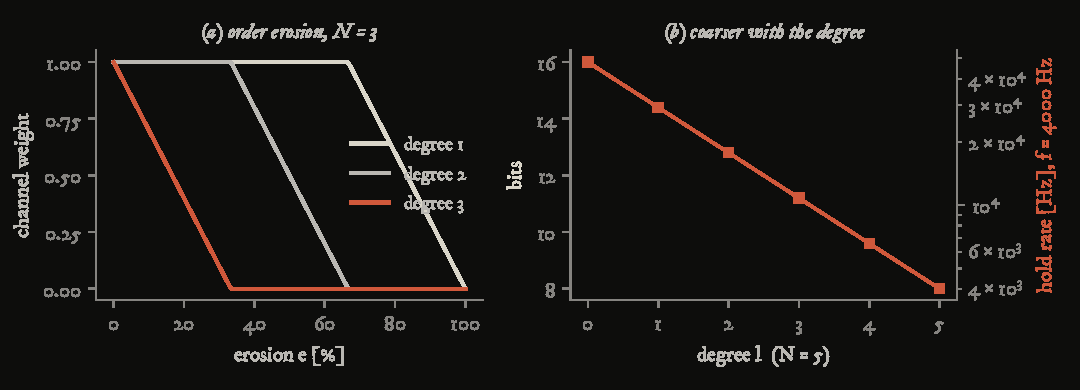
\includegraphics[width=0.95\linewidth]{figs/spacedeg.pdf}
\caption{Spatial degradation. (a) \ui{Ordnung abtragen}: the weight of each degree $l$ for $N=3$ falls from the
top, continuously. (b) \ui{Raum-Bittiefe} and \ui{Raum-Abtastrate}: the higher the degree, the coarser (here
$B=8$ and $f_h=\SI{4}{kHz}$ at $N=5$); $W$ stays clean.}
\label{fig:spacedeg}
\end{figure}

\begin{description}[style=nextline,leftmargin=1.2em]
\item[{\ui{Ordnung abtragen} (erosion $e\in[0,1]$).}] The channels of degree $l$ are multiplied by
  $w_l=\mathrm{clip}\bigl(N(1-e)-(l-1),0,1\bigr)$: the highest order fades out first, continuously between the
  orders (50\,\% of third order leaves the first order complete, the second at half and the third gone). At
  $e=1$ only $W$ remains: everything sounds from everywhere. The weights are interpolated linearly over
  each block.
\item[{\ui{Verwittern} (weathering).}] A time $T$ after which the sphere is completely eroded while something
  sounds. An internal age $a$ rises by one second per second of sound and falls four times as fast in silence;
  the erosion heard is $\mathrm{clip}(e + a/T,0,1)$, shown in the title.
\item[{\ui{Richtungsraster} (grid $g$).}] Every direction snaps to the nearest of $n_g=\mathrm{clip}\bigl(\mathrm{round}(64(1-g)^2+4g),4,64\bigr)$ points
  spread evenly over the sphere (Fibonacci lattice): moving pipes jump from point to point. Also in stereo.
\item[{\ui{Raum-Bittiefe}, \ui{Raum-Abtastrate}.}] Rounding to $2^{b_l-1}$ steps and sample-and-hold at $f_l$ per
  degree, with
  $b_l = 16-(16-B)\,l/N$ and $f_l = 48\,000\,(f_h/48\,000)^{l/N}\ge\SI{60}{Hz}$:
  the fine directional detail decays first, $W$ stays clean.
\item[{\ui{Raum-Aussetzer} (drops $d$).}] Single channels, or in 30\,\% of the cases a whole degree, fall out for
  \SIrange{50}{400}{ms} (\SI{5}{ms} ramps). Checked every 64 samples with probability proportional to $d^2$
  (up to 3 per second and channel): the sound tips to one side or goes flat for a moment.
\item[{\ui{Raum-Aliasing} (alias $\alpha$).}] The field is \emph{sampled at too few points and encoded again}.
  With $K=\max\bigl(4,\mathrm{round}((N+1)^2(1-0.85\alpha))\bigr)$ directions $\boldsymbol\theta_k$ of a Fibonacci lattice
  the channels pass through
  \begin{equation}
    \mathbf M=\frac1K\sum_{k=1}^{K}\mathbf y(\boldsymbol\theta_k)\,\bigl(\mathbf w\circ\mathbf y(\boldsymbol\theta_k)\bigr)^{\!\top},\qquad w_c=2l_c+1,
  \end{equation}
  which for $K\ge(N+1)^2$ points is the identity (the SN3D quadrature) and for fewer points leaves ghost
  directions. The output is $\mathbf x+\min(1,2\alpha)\,(\mathbf M\mathbf x-\mathbf x)$. The lattice turns at \SI{7}{\degree\per\second}
  and $\mathbf M$ is rebuilt every 1024 samples, so the ghosts wander slowly.
\end{description}
The erosion and the aliasing are the only parts that are not per-channel; all the others use a state per
Ambisonics channel (held value, phase, drop gain, drop counter), so the cost is a few operations per channel
and sample.

\emph{Status:} like the loudspeaker decoder this was added after the verification run of 1~November and is described from the
source code and the README. The render test of 15~November checks erosion, grid, crushing, dropouts, aliasing and weathering
(\S\ref{sec:verification}); for example at 50\,\% erosion degree~2 is \SI{6}{dB} down and degree~3 gone, while degrees 0 and 1 are untouched.

\subsection{Glitches (\ui{Verfall $\cdot$ Glitch})}
\label{sec:glitch}
The third tab of the \ui{Verfall} section imitates a failing playback rather than a worn recording. All four act
on every pipe separately (\fn{GlitchParams}), are off by default and are per-pipe modulation targets.
\begin{description}[style=nextline,leftmargin=1.2em]
\item[{\ui{Stottern} (stutter).}] At random moments (a Poisson process with rate $2.5\,s^2$ per second) a slice of
  \SIrange{20}{150}{ms} of the pipe jumps back to its start two to six times, like a hanging buffer.
\item[{\ui{Bandschnitt} (tape splice).}] The crossfade at the loop points shrinks to $(1-s)$ of its length, and each
  pass through the loop adds a tick and a short dip of \SI{12}{ms}: the loop becomes an audible splice.
\item[{\ui{Harte Kanten} (hard edges).}] No care for zero crossings: a note may start anywhere in its first moments, and the
  release ramp of \SI{40}{ms} shrinks to almost nothing, so notes end in a hard cut.
\item[{\ui{Clipping}.}] Bursts of \SIrange{8}{80}{ms} (Poisson rate $3c^2$ per second) in which the pipe is driven by a
  factor of 4 to $4+30c$ into a hard limit, level-compensated.
\end{description}

% =====================================================================
\section{Tuning}
\label{sec:tuning}
% =====================================================================

The recorded pipes are in quarter-comma meantone. Every other tuning is reached by shifting pipes, with
$a'$ always kept at its pitch; \ui{Stimmton} moves the whole organ by $\pm\SI{200}{ct}$ (displayed as
A4 in Hz), and \ui{Verstimmung} gives every pipe a fixed random detune of up to \SI{60}{ct}.

\paragraph{Twelve-note tunings.} For a temperament with pitch classes $t_i$ (cents above C), the
pipe of pitch class $i$ is shifted by
\begin{equation}
  \Delta_i = (t_i - t_9) - (c_i - c_9),
\end{equation}
with $c_i$ the meantone values of Eq.~\eqref{eq:meantone}. Available are the historical temperaments
(\nicefrac14- and \nicefrac16-comma meantone, Werckmeister~III, Kirnberger~III, Vallotti, Pythagorean,
equal; Figure~\ref{fig:temperaments}) and exotic twelve-note scales: 5-limit just intonation on C,
septimal 7-limit just intonation, the harmonic series on C (partials 16--30), twelve notes out of 31-,
19- and 53-EDO, and Maqam Rast (E and B a quarter tone low).

\begin{figure}[h]
\centering
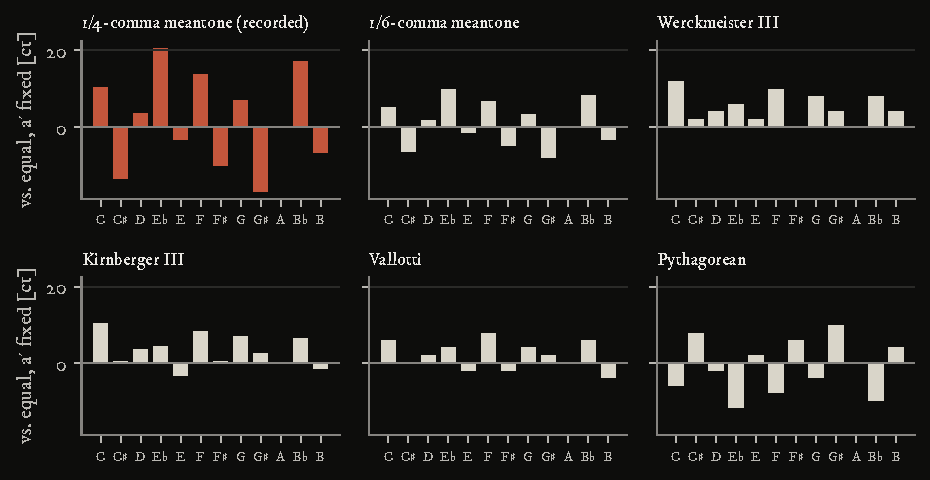
\includegraphics[width=\linewidth]{figs/temperaments.pdf}
\caption{Historical temperaments available in the plug-in, as deviation from equal temperament with $a'$
fixed. The recorded quarter-comma meantone is shown in orange; all others are reached by shifting each
pitch class by the difference.}
\label{fig:temperaments}
\end{figure}

\paragraph{Step tunings.} In the step tunings every MIDI note is one step of a scale with step size
$s$: 31-EDO (\SI{38.7}{ct}), 19-EDO (\SI{63.2}{ct}), quarter tones (\SI{50}{ct}), Bohlen--Pierce
(13 steps per twelfth, \SI{146.3}{ct}) and Wendy Carlos' Alpha (\SI{78.0}{ct}). The target of key $k$ is
$(n_k-69)\,s$ cents from $a'$. Instead of shifting the pipe of key $k$ by possibly many semitones, the
engine plays the \emph{recorded pipe whose pitch is closest to the target} and shifts it by the
remainder. Each pipe therefore keeps its timbre and its place in space, and no pipe is shifted by more
than about half a recorded step (31-EDO: at most \SI{40}{ct}).

\paragraph{Free tuning: Scala and MTS-ESP.} The last two entries of the tuning list give every MIDI note
$0\dots127$ on every channel its own frequency, held in a $16\times128$ table:
\begin{itemize}
  \item \emph{Scala} \citep{scala}: a \code{.scl} file (degrees in cents or ratios) and optionally a
        \code{.kbm} keyboard mapping (which key plays which degree, unmapped keys, reference key and
        frequency). Without a \code{.kbm} the default maps degree 0 to note 60 (C4) at \SI{261.625565}{Hz}, the C of 12-tone equal
        temperament at A4 $=\SI{440}{Hz}$; with no scale loaded the entry plays exactly that. (Earlier versions put
        note 69 at \SI{444.5}{Hz} to match the organ; the default has changed.) The \ui{Stimmton} row then shows the
        reference note and frequency of the \code{.kbm}, or of this default, and the tuning uses these absolute
        frequencies independently of the \ui{Stimmton} setting. \ui{KBM entfernen} goes back to the default mapping. The
        file contents are stored in the project and in patches.
  \item \emph{MTS-ESP} \citep{mtsesp}: the plug-in follows an MTS-ESP master (including multi-channel
        tables for keyboards with more than 128 keys and unmapped keys). Without a master it reads
        MIDI Tuning Standard SysEx \citep{mts1992} from the MIDI input, as sent by isomorphic-keyboard
        tools such as Hexatone. \ui{Töne folgen} lets held notes follow tuning changes (off: every note keeps the pitch it
        was struck with); in this mode it replaces the \ui{Stimmton} row. Until a master is connected or SysEx has arrived the
        entry plays calibrated 12-tone equal temperament at A4 $=\SI{440}{Hz}$, independent of the stored \ui{Stimmton}; the
        status line names this fallback and shows \emph{MIDI Tuning (MTS-ESP) empfangen} once a table has arrived.
        (Ableton Live does not pass SysEx to plug-ins; there an MTS-ESP master is needed.)
\end{itemize}
For each note the nearest recorded pipe plays, shifted by the rest; notes beyond the compass are shifted
from the outermost pipes by up to two octaves. Notes that land on the same pipe each get their own voice,
so clusters and fine microtonal steps are possible.

\paragraph{Calibrated sample pitch and the extended range.} The recorded pipes are not exactly in tune with their nominal
pitch: the measured values scatter by a few cents (\S\ref{sec:measured}). With \ui{Original} (the recorded quarter-comma
meantone) the samples play as recorded, at their native rate; with \emph{every other} tuning (historical, exotic, step,
Scala, MTS) the engine corrects the playback rate so that a pipe lands exactly on the frequency the tuning asks for. The
preprocessing stores for each pipe the frequency $f_\text{cal}$ of the raw sample, checked against the measurement. With
the nominal meantone frequency $f_\text{mt}(n)$ of the pipe's key (Eq.~\ref{eq:meantone}), the footage factor $m$ of the stop
(8$'$: 1, 4$'$: 2, 2$'$: 4, 16$'$: $\tfrac12$) and the rates $f_{s}$ of the file and $f_{s,\text{out}}$ of the host,
\begin{equation}
  \rho = \frac{f_{s}}{f_{s,\text{out}}}\cdot\frac{f_\text{target}}{f_\text{cal}}\cdot m,
  \qquad\text{and a calibration ratio } \frac{f_\text{mt}(n)\, m}{f_\text{cal}} \text{ for the voice stage,}
\end{equation}
so a pipe that was recorded \SI{4}{ct} flat no longer plays \SI{4}{ct} flat in a just or microtonal scale
(\fn{SamplePitch.h}). A pipe or a stop whose calibration is missing is not corrected, and one whose figures are not
finite plays at its native rate or not at all rather than at a wrong pitch. In the same modes every MIDI note inside the
compass gets a pitch, also those that the organ has no key for (its keyboard table is filled on the audio thread), and a new
switch \ui{Erweiterter Bereich} on the \ui{Klang} page extends this to MIDI notes 24--108, played from the outermost pipes.
The switch is stored with the project and has no effect in \ui{Original}.

\subsection{A reference tone for the ear (\ui{Testton})}
\label{sec:testton}
To compare the pitch of the samples by ear the plug-in has an independent, dry reference tone (\fn{Dsf*.h}, the box
\ui{Testton} on the \ui{Klang} page and a button on the \ui{Spieltisch}). It is not a pipe and does not go through the voice
stage, the room or the effects; it is added after them, to the W channel when the output is Ambisonic (before the binaural or loudspeaker decoder, which then
play it as an omnidirectional source) and to both channels in stereo. It is built to be as free of errors as possible:
\begin{itemize}
  \item \ui{MIDI} on: it plays the last held MIDI note in the tuning that is selected, with the global \ui{Stimmton} and an own
        \ui{Feinstimmung} of $\pm\SI{50}{ct}$ (resolution \SI{0.01}{ct}), sustain pedal, pitch wheel and MPE included. In
        \ui{Original} tuning it follows the \emph{recorded} frequency of the chosen \ui{Register} (one of six stops, or
        the nominal quarter-comma meantone at A $=\SI{444.5}{Hz}$) -- so one hears the pipe and the tone one after the other
        on exactly the same pitch. \ui{MIDI} off: a continuous frequency \ui{Frequenz} of \SIrange{20}{20000}{Hz}.
  \item \ui{Oktavlage} $32'\dots2'$ and \ui{Mixtur} $1\dots9$ shift the tone by whole octaves or by the $m$-th harmonic
        ($+1200\log_2 m$ ct), to compare it with a stop of another register.
  \item \ui{Spektrum} $x\in[0,1]$ moves from a sine to the full spectrum of a sawtooth with up to \ui{Teiltöne} $=1\dots1024$
        partials, \ui{Pegel} is \SIrange{-60}{-6}{dB} (default \SI{-32}{dB}).
\end{itemize}
The tone is a \emph{discrete summation formula} (DSF) oscillator. A DSF sums a geometric series of partials in closed form; here
the series of cosines is
$\sum_{n=1}^{N} r^{n-1}\cos n\phi$, computed from $\mathrm{Re}\,(e^{i\phi}(1-(re^{i\phi})^N)/(1-re^{i\phi}))$ (a finite sum is used
where the denominator comes near zero), and it is \emph{integrated} sample by sample to give partials
$r^{n-1}\sin(n\phi)/n$, that is a sine at $r=0$ and the $1/n$ of a sawtooth at $r=1$. The slider is bent so that the useful range of
$r$ is spread out, $r = 1-(1-x)^2$ (Fig.~\ref{fig:dsf}, left). The integrator is the trapezoidal rule (the \ui{Integration} choice
in the saved state is only kept for compatibility); it multiplies partial $n$ by $\tan(\theta/2)/\tan(n\theta/2)$ instead of $1/n$, for the phase
step $\theta=2\pi f/f_s$ per sample. This error is small only far below Nyquist; it is limited by oversampling the oscillator
by 1, 2, 4 or 8 and choosing the smallest factor for which the highest partial is correct to \SI{0.25}{dB} (\fn{chooseDsfOversampling}),
with partials above $0.45\,f_s$ dropped. The \emph{continuous} tone, whose frequency can be swept, always reserves the factor of 8
and filters down with an oversampling filter; when a sweep changes the spectrum the integration constant is rebuilt, so no DC offset arises,
and a change of the number of partials is cross-faded in \SI{30}{ms}.

\begin{figure}[ht]
\centering
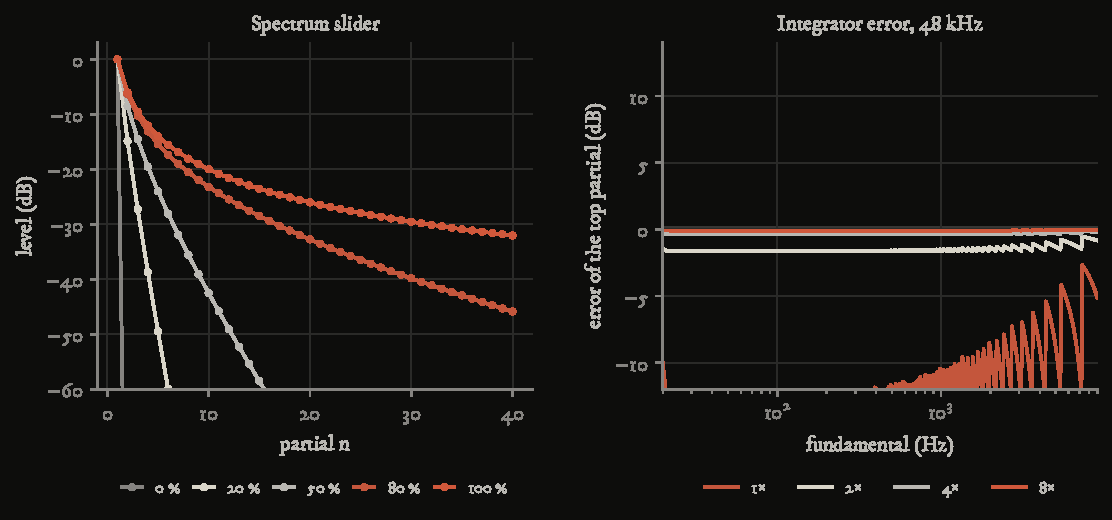
\includegraphics[width=\linewidth]{figs/dsf.pdf}
\caption{The reference tone, computed with the rules of \fn{DsfMath.h} and \fn{DsfOversampling.h}. Left: level of the partials for
five positions of \ui{Spektrum}; the slider is bent, $r=1-(1-x)^2$. Right: error of the highest partial for the integrator at $f_s=\SI{48}{kHz}$
with 1, 2, 4 and 8 times oversampling (blank where the partial would pass Nyquist); grey: the $\pm\SI{0.25}{dB}$ that the plug-in allows.
At 8$\times$ the error stays within \SI{0.1}{dB} from \SI{20}{Hz} to \SI{9}{kHz}.}
\label{fig:dsf}
\end{figure}

% =====================================================================
\section{Spatialisation}
\label{sec:spatial}
% =====================================================================

\subsection{Conventions}
Positions are given as azimuth $\varphi$ (0° = front, +90° = left), elevation $\vartheta$
(0° = horizon, +90° = zenith) and distance $r$ in metres (\SIrange{0.5}{60}{m}), following the AmbiX
convention \citep{nachbar2011ambix} used by the IEM suite and Reaper.

\subsection{Ambisonics encoder}
Every pipe is encoded with real spherical harmonics in ACN channel order and SN3D normalisation without
Condon--Shortley phase (AmbiX) up to order $N\le5$:
\begin{equation}
  Y_n^m(\varphi,\vartheta) = \sqrt{(2-\delta_{m0})\,\frac{(n-|m|)!}{(n+|m|)!}}\;
  P_n^{|m|}(\sin\vartheta)\;
  \begin{cases}\cos(m\varphi) & m>0\\ 1 & m=0\\ \sin(|m|\varphi) & m<0\end{cases},
  \qquad \text{ACN} = n^2+n+m,
\end{equation}
where $P_n^m$ are the associated Legendre functions, computed by the standard recurrences
\citep{zotter2019}. The encoded pipe signal is $\mathbf{y}(t) = g(t)\,s(t)\,\mathbf{Y}(\varphi,\vartheta)$,
with the gains recomputed every 64 samples and ramped in between.

\subsection{Stereo}
In stereo mode the azimuth is mapped to an equal-power pan (front and back fold onto the same position):
\begin{equation}
  p = \sin\varphi,\qquad \alpha = \tfrac{\pi}{4}(1-p),\qquad g_L=\cos\alpha,\quad g_R=\sin\alpha .
\end{equation}

\subsection{Distance}
\label{sec:distance}
Distance acts in three ways. The level follows
\begin{equation}
  g_r = \min\!\left(4,\ \left(\frac{\SI{4}{m}}{\max(\SI{0.5}{m},r)}\right)^{\!a}\right),
\end{equation}
where $a\in[0,1]$ (\ui{Entfernung $\rightarrow$ Lautstärke}) blends between no distance effect and $1/r$.
Air absorption (\ui{Luft}) is a one-pole low-pass with corner
$f_c = \operatorname{clamp}\bigl(20000/(1+\text{air}\cdot r/5),\,1200,\,20000\bigr)$\,Hz.
\ui{Luft umkehren} $u\in[0,1]$ turns this around: the output is $y_\text{air}+2u\,(y-y_\text{air})$, where $y_\text{air}$ is the
signal after and $y$ before the air low-pass. At $u=0.5$ the highs the air took away are restored (far pipes
sound as bright as near ones), at $u=1$ they are exaggerated, so the farther a pipe, the brighter -- a distant presence
that does not exist in nature. A change of distance
produces a Doppler shift (\ui{Doppler}, factor $D_s\in[0,4]$, 1 = physical),
\begin{equation}
  D = \operatorname{clamp}\!\left(\frac{c}{c + D_s\,v_r},\ 0.5,\ 2\right),\qquad
  v_r = \frac{\Delta r}{\Delta t},
\end{equation}
with the radial velocity $v_r$ limited to $\pm\SI{120}{m/s}$. Pipes that jump (below) never glide, so
they have no Doppler. Far pipes also send relatively more to the room: the room send falls only with
$0.35a$ instead of $a$.

\subsection{Layouts}
\label{sec:layouts}
The \ui{Raum} page places all pipes of a stop at once with a layout generator (width, centre, height,
spread and distance; all of them continuous -- \ui{Abstand}, \SIrange{1}{40}{m}, used to move in steps of half a metre):
\begin{description}
  \item[Gehäuse C/C♯] as in an organ case: semitones alternate between a C side and a C♯ side, bass in the
        middle, treble towards the outside;
  \item[Tonhöhe] pitch from one side to the other;
  \item[Streuung] random scatter (direction and distance);
  \item[Ring] a full circle around the listener;
  \item[Spirale] two turns, rising and approaching;
  \item[Zone] a small cloud around one direction;
  \item[Tonnetz] every key at its place in the lattice of the tuning in use (below).
\end{description}

\paragraph{Tonnetz.} The tuning decides the map (\fn{tonnetzPlaces}, \fn{Spatial.h}). From the twelve pitch classes of
the tuning the median fifth $F$ and median major third $T$ are taken (for step tunings the nearest multiples of the
step). Each key, with pitch class $p$, is placed at the lattice point $(a,b)$, $|a|\le8$ fifths and $|b|\le2$ thirds,
that minimises
\begin{gather}
  C(a,b)=|a|\,w_F+|b|\,w_T+\tfrac13\,d_{1200}\bigl(aF+bT,\;p\bigr),\\
  w_F=0.5+\tfrac{|F-701.955|}{4},\qquad w_T=0.5+\tfrac{|T-386.314|}{4},\notag
\end{gather}
where $d_{1200}$ is the distance of two pitch classes in cents ($\le600$),
so that pure intervals are cheap and impure ones expensive. One fifth is drawn
$s_F=0.7+|F-701.955|/10$ units long, one third $s_T=0.7+|T-386.314|/10$: impure intervals look long. Fifths go to the
right, thirds upwards and half a step to the right (the triangles of the Tonnetz); octaves add a little height and come
nearer. In ¼-comma meantone the triads form tight groups and G♯ and E♭ end up on opposite edges -- the wolf is the
seam; in Pythagorean tuning the keys line up as one chain of fifths; in equal temperament the thirds are drawn long
(Figure~\ref{fig:tonnetz}). A stop arranged as a Tonnetz is redrawn when the tuning changes.

\begin{figure}[t]
\centering
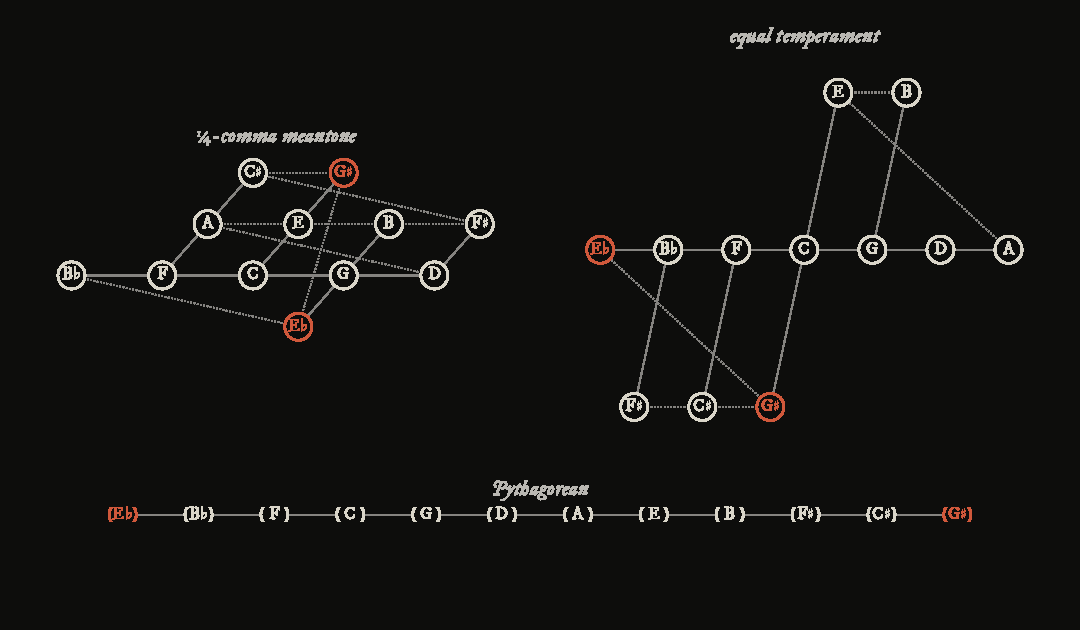
\includegraphics[width=0.9\linewidth]{figs/tonnetz.pdf}
\caption{The Tonnetz layout for one octave, computed with the rule of \fn{tonnetzPlaces}: dotted lines are fifths,
solid lines major thirds (drawn only between neighbours). Red: G♯ and E♭, the two ends of the meantone chain.}
\label{fig:tonnetz}
\end{figure}
Single pipes can be dragged, a whole stop can be rotated, and pipes can be muted individually.

\subsection{Motion}
\label{sec:motion}
Each stop has a motion mode and a speed from $-500$ to $+\SI{500}{Hz}$ (with a strongly skewed knob for
fine control at slow speeds; negative = the other direction). The engine integrates the speed into a
phase $\Phi$ in cycles, so changing the speed never makes the position jump and smooth speed glissandi
are possible. Optionally the phase is locked to the host tempo and song position (speeds are then
interpreted at \SI{120}{BPM}). With position updates every 64 samples the motion itself begins to alias
above roughly \SI{300}{Hz} -- an effect that is kept as a sound of its own.

\begin{description}
  \item[Statisch] no motion.
  \item[Rotation] $\varphi' = \varphi + 360°\,\{\Phi\}$ (fractional part).
  \item[Pendel] $\varphi' = \varphi + \delta\sin(2\pi\Phi)$, depth $\delta$.
  \item[Drift] smooth pseudo-random wandering of azimuth, elevation and distance (sum of three
        sines with per-pipe random rates and phases).
  \item[Vertikal] rotation about the left--right axis: front $\rightarrow$ up $\rightarrow$ back
        $\rightarrow$ down.
  \item[Sprünge] every pipe jumps to a new random place around its position once per cycle, each at its
        own moment. Jumps glide over about \SI{4}{ms} so they do not click; with \ui{harte Sprünge} the
        gains are switched at the exact sample, which clicks and, from about \SI{50}{Hz}, buzzes.
  \item[Schwebung] every pipe turns around the listener as fast as it beats with the other sounding pipes
        (\S\ref{sec:beats}); \ui{Geschwindigkeit} is the number of turns per beat. A pipe whose intervals are pure stands
        still where it is.
  \item[Gezeichnet] a trajectory drawn in the top view (up to 256 points with their drawing times). The
        pipes travel along it like a train; \ui{Verteilung auf der Bahn} spreads them along the path
        (0 = all together, 1 = spread over the whole path in keyboard order), \ui{Schleife} or
        \ui{Hin \& zurück} and \ui{gleichmäßig} or \ui{Zeichentempo} (as fast as it was drawn) choose
        how the path is run.
  \item[Flug, Fall, Schwarm, Strömung, Schweben] five further modes, shown in the interface as a row \ui{im Saal} beside the modes above.
        Here a pipe is no longer a direction around the listener but a body with a place and a speed in the room
        (\S\ref{sec:roommotion}).
\end{description}

\paragraph{A speed for every pipe (\ui{Tempo-Streuung}).} By default all pipes of a stop share the stop's phase, so a ring turns as one. The
per-stop control \ui{Tempo-Streuung} $\sigma\in[0,1]$ (tab \ui{Pfeife} of the \ui{Raum} page, \S\ref{sec:stopfx}) gives every pipe $k$ a phase of its own,
\begin{equation}
  \Phi_k=\Phi\,(1+\sigma\,r_k)+o_k,\qquad r_k\in[-1,1]\ \text{a fixed hash of stop and key},
\end{equation}
which drives \ui{Rotation}, \ui{Vertikal}, \ui{Pendel} and \ui{Drift}: at $\sigma=1$ the pipes run between standing still and twice the stop's speed, and
a circle becomes a swarm that pulls apart. When $\sigma$ changes from $\sigma_0$ to $\sigma_1$, the offset $o_k$ grows by $\Phi\,r_k(\sigma_0-\sigma_1)$,
so that $\Phi_k$ is unchanged at that moment: changing the spread changes only the speeds and never makes a pipe jump. Because $\Phi_k$ is derived from
the stop's phase, listeners of a concert (\S\ref{sec:konzert}) follow it from the phase they receive.

\paragraph{Orbit shape.} For every mode an \ui{Ellipse} turns the orbit into an elliptical or lobed one,
which produces distance changes and therefore Doppler. With amount $e$, direction $\varphi_e$, number of
near sides $k\in\{1,2,3,4\}$ (\ui{Form}) and tilt $\tau$ (\ui{Neigung}):
\begin{align}
  r' &= r\bigl(1 - e\,\cos\vartheta\,\cos(k(\varphi-\varphi_e))\bigr),\\
  \vartheta' &= \vartheta + \tau\cos(\varphi-\varphi_e)\cos\vartheta .
\end{align}
$k=1$ places the listener at a focus, $k=2$ in the centre, $k=3,4$ give triangle- and square-like orbits
(Figure~\ref{fig:orbits}).

\begin{figure}[h]
\centering
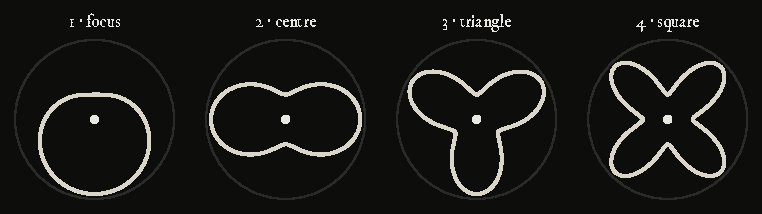
\includegraphics[width=0.92\linewidth]{figs/orbits.pdf}
\caption{Orbit shapes (\ui{Form} 1--4) for an ellipse amount of 50\,\%, seen from above, front up; the dot
is the listener.}
\label{fig:orbits}
\end{figure}

\subsection{Pipes as bodies in the room (\ui{Flug, Fall, Schwarm, Strömung})}
\label{sec:roommotion}
The motions above turn a pipe around the listener, so the pipe always stays on the sphere (or the ellipse) around the
listening place. In five further modes, which the interface groups in a row \ui{im Saal}, every pipe becomes a
\emph{body} with a position and a velocity inside the Saal of its stop (its floor plan, floor and ceiling,
\S\ref{sec:plans}; the room is that of the stop also when \ui{Saal an} is off). The pipe starts where it was, with the
speed asked for, and from then on is heard, reflected and hidden behind corners (\S\ref{sec:walk}) from where it
really is, Doppler shift included. \ui{Geschwindigkeit} is a speed in the room: \SI{1}{Hz} is \SI{10}{m/s}, at most
\SI{40}{m/s}; with \ui{Sync} it grows with the tempo but is not locked to the bar. \ui{Tiefe} has a meaning of its own in
every mode.
\begin{description}
  \item[Flug] straight lines; a pipe bounces off the walls, the floor and the ceiling without loss. \ui{Tiefe}: how
        roughly the walls throw it off.
  \item[Fall] gravity ($g=\SI{9.81}{m/s^2}$). The pipes fall, bounce on the floor with their whole length (a long pipe
        stands tall), slide to a halt and, after a resting time of \SIrange{0.8}{2.3}{s}, are thrown up again;
        \ui{Geschwindigkeit} is how hard. \ui{Tiefe} sets the bounce: the coefficient of restitution is $0.3+0.65\,d$.
  \item[Schwarm] the pipes of the stop flock: together (towards the middle of the flock), in one direction (towards its
        mean heading) and never too close to each other. \ui{Tiefe}: how much every pipe wants its own way.
  \item[Strömung] a slow current through the room, smooth in space and time, carries the pipes. \ui{Tiefe}: turbulence.
  \item[Schweben] the pipes hover where they started. The air slows them, and a pull
        $2.5\,(1-d)^2$ per second$^2$ per metre ($d$: \ui{Tiefe}) draws them back to the starting place, so at full depth nothing calls them back and they drift
        free; \ui{Geschwindigkeit} is a slight unrest of their own ($0.25$ times the speed as a random acceleration). The
        walls return $0.7$ of the speed. The mode is made for \emph{the player} (below): a pipe stays where it is until
        the listener pushes or pulls it.
\end{description}
The bodies are integrated in fixed steps of $1/480$\,s, with the remainder carried over, and the steps are counted in
whole samples, so that the same paths and the same impacts arise at every buffer size. A pipe keeps a margin of
\SI{0.25}{m} from the walls. The size of a pipe follows its pitch: with the footage $f$ of the stop in feet and the key
index $k$ (0 is the lowest key, C) its length is $\ell = 2.44\,\mathrm{m}\cdot f/8\cdot
2^{-k/12}$, halved for the Gedackt, and its radius $0.035\,\ell$ ($0.07\,\ell$ stopped).

\paragraph{Aufprall (impacts).} Where a pipe hits a wall, the floor or the ceiling it knocks. The switch is
\ui{Aufprall} on the \ui{Effekte} page, tab \ui{Lebendige Orgel} (\S\ref{sec:live}), with \ui{Lautstärke} (off by
default), \ui{von} \emph{klingenden} or \emph{allen Pfeifen} and \ui{Nachklang des Rohrs}. An impact is synthesised, not
sampled, by a pool of 32 voices (at most 24 events per block; the weakest gives way). It consists of three parts:
\begin{enumerate}
  \item the \emph{contact}, a raised-cosine pulse whose length falls with the speed of the hit, so that a harder hit
        is shorter and brighter (a short contact excites the higher modes of the tube), plus a little clatter of noise
        whose cutoff rises from \SI{0.7}{kHz} to about \SI{11.7}{kHz} with the speed;
  \item the struck pipe, ringing in the four bending modes of a free tube with the frequency ratios
        $1:2.756:5.404:8.933$ above a lowest mode $f_1 = 300\,\mathrm{Hz}\cdot\ell^{-1.5}$ (with $\ell$ in metres, limited to
        \SIrange{35}{2500}{Hz}), decaying faster for the higher modes, and faintly at its own note (a fifth mode);
        the Trompete rings a little longer ($\times1.2$). Since 14~November the Gedackt is of wood: its contact is three times
        longer, its clatter quieter ($\times0.35$) and duller ($\times0.3$ in cutoff), its modes lower ($\times0.7$, the upper ones weaker) and
        far shorter ($\times0.12$), and a dry, woody resonance of the hollow box is added, gone within a few hundredths of a second;
  \item the wall itself, a dull thump (\SI{110}{Hz} for the floor, \SI{180}{Hz} for walls), stronger for the floor.
\end{enumerate}
The surface's absorption and high damping, taken from the Saal (and, with single materials per surface, from the surface that is hit, \S\ref{sec:surfaces}), make the knock quieter and duller; below a speed of
\SI{0.25}{m/s} a pipe only touches and does not knock. Every knock comes from the place where it happened and also goes
into the room; in the 3D view (\S\ref{sec:walk}) it flashes. When a pipe of the wooden Gedackt knocks, it sounds dull and short (\S\ref{sec:walkgpu}).
Like the living organ, this part was written after the verification run of 1~November; the run of 15~November covers it (the four motions in a
cross-shaped plan keep every pipe inside the walls, a knock at \SI{6}{m/s} is \SI{25}{dB} louder and brighter than one at \SI{1}{m/s}, a curtain
takes \SI{5}{dB} of it, and the paths and impacts are the same at block sizes 64 and 512).

\subsection{Grain cloud (\ui{Wolke})}
\label{sec:cloud}
On the \ui{Raum} page a third tab (next to \ui{Bewegung} and \ui{Hall}) gives every stop a \emph{grain cloud}.
Every sounding pipe of the stop scatters grains of its own sound over the sphere around the pipe's position
(\fn{CloudParams}): \ui{Menge} (mix, equal power: at 100\,\% only grains are left), \ui{Dichte} (30 grains per
second and pipe by default), \ui{Streuung} (the angle around the pipe: a few degrees give a shimmering spot,
$\SI{180}{\degree}$ the whole sphere), \ui{Korngröße} (Hann-windowed, $\pm30\,\%$, \SI{80}{ms} by default) and
\ui{Zeitstreuung} (how far back in the pipe's own sound a grain may reach, up to \SI{150}{ms}, which smears attacks
and movement). The cloud follows the pipe's motion; the grains are not sent to the room separately, the pipe's room
send is unchanged. Up to 64 pipes at a time have a cloud (256 grains in all), more stay whole.
\ui{für alle Register übernehmen} copies the five values to every stop. This part is described from the
source code and README; the render test of 15~November checks that the cloud spreads the energy over the sphere (the length of the
energy vector $r_E$ falls from 1 to 0.11 for the whole sphere and stays 0.98 at \SI{15}{\degree}) at an unchanged level.

\subsection{Binaural rendering}
\label{sec:binaural}
For headphones (and hosts with stereo tracks only, such as Ableton Live) the plug-in renders Ambisonics
internally (order 1--5, default 3) and decodes it to two ears. The decoder is designed like the IEM
BinauralDecoder \citep{iemsuite} with magnitude least squares (MagLS) \citep{schoerkhuber2018magls}:
below a cutoff of about $\SI{620}{Hz}\times N$ the HRTFs are fitted with spherical harmonics in the
ordinary least-squares sense, which keeps interaural time differences correct; above it only the
magnitudes are fitted and the phase is taken from the previous frequency, since it cannot be represented
at low orders anyway. The diffuse-field energy of the fit is then matched to that of the HRTFs, and
optionally the whole set is diffuse-field equalised (minimum phase) for headphones that are themselves
diffuse-field tuned. Finally the level is set so that a diffuse field reaches each ear at \SI{-3}{dB},
like an equal-power stereo pan.

The built-in HRTF set is the FABIAN head-and-torso simulator of TU Berlin \citep{brinkmann2017fabian}
(CC BY 4.0), reduced to 2000 of its 11\,950 directions. Any SOFA file \citep{majdak2013sofa} of the
convention \code{SimpleFreeFieldHRIR} can be loaded instead, for example an individual measurement. The
design runs in a background thread (\SIrange{0.3}{0.4}{s}) whenever order, HRTF set or sample rate change.
The real-time part is a partitioned convolution (\S\ref{sec:perf}) with a single stage of block size 128
(hence \SI{128}{samples} of latency) of up to 36 channels into two; a head rotation (\ui{Kopfdrehung}, also a modulation target) is
applied to the Ambisonics signal before decoding.

\subsection{Two loudspeakers (transaural)}
\label{sec:transaural}
The output \ui{Transaural (2 LS)} (also the switch \ui{Transaural an} in the box \ui{Zwei Lautsprecher} on the \ui{Klang}
page) plays the binaural signal over a pair of loudspeakers. It is the binaural decoder of the previous section --
same Ambisonics order, same HRTF set (FABIAN or an own SOFA file), \ui{Kopfdrehung} and diffuse-field equalisation --
followed by a \emph{crosstalk cancellation} (\fn{Transaural.h}). Each loudspeaker also reaches the far ear, a little
later (the interaural time difference) and quieter (the head shadow). With the two loudspeakers placed symmetrically at
$\pm\alpha$ to the listener, the transfer from the speaker pair to the two ears is, per frequency, $H_n\bigl(\begin{smallmatrix}1&R\\R&1\end{smallmatrix}\bigr)$ with
the near-ear response $H_n$ and the ratio $R$ of far ear to near ear. This matrix is diagonalised by the sum and the
difference of the two channels, so its inverse splits into two filters:
\begin{equation}
  C_s = \frac{1}{1+R}\ \text{on}\ \frac{L+R}{2},\qquad C_d = \frac{1}{1-R}\ \text{on}\ \frac{L-R}{2},\qquad
  \text{left} = m' + s',\ \ \text{right} = m' - s'.
\end{equation}
$R$ is not modelled but read from the HRTF set in use, at the angle of the speakers: the measured complex ratio of the
far to the near ear, with the interaural delay (the lag at which the far-ear response fits the near-ear one best)
taken out, smoothed over $1/12$ octave in real and imaginary part and limited to a magnitude of 0.97; the delay is put
back afterwards. (A pure delay alone cancels only about \SI{6}{dB}, because the sound bends around the head and its
delay to the far ear changes with frequency.) At low frequencies $1-R$ becomes small, since the head is small against the
wavelength, and the full inverse would boost the side signal there without limit. The inverse is therefore regularised,
$C_x = \bar X/(|X|^2+\beta)$ with $X = 1\pm R$, so that no frequency is boosted by more than \ui{höchste Anhebung}
(\SIrange{3}{20}{dB}, default \SI{10}{dB}); below about \SI{80}{Hz} and above about \SI{12}{kHz}, where cancellation does
not work (the ears are too close in wavelengths, or the head is never exactly where it was measured) the filters fade
to plain. The remaining controls are
\begin{itemize}
  \item \ui{Lautsprecher bei} $\pm10\dots150°$ (default $\pm90°$: the two speakers on opposite sides of the room, facing each
        other, the listener in the middle -- a good layout because the head already shades each ear from the far speaker);
  \item \ui{Übersprechen aus} \SIrange{0}{100}{\percent}: 0 is the binaural signal plainly over the speakers, 100 is full
        cancellation, which is more spatial and more sensitive to where one sits;
  \item \ui{Seitenklang ausgleichen}: also takes out the colour of the speakers' own direction (the near-ear HRTF at the
        angle, smoothed over $1/3$ octave, at most $\pm\SI{10}{dB}$), so the ears receive the binaural signal and not
        binaural times the HRTF of the side.
\end{itemize}
The filters are designed in a background thread (a few hundred milliseconds) whenever angle, amount, boost, the HRTF set or the
sample rate change, and cross-faded in; they add \SI{5.3}{ms} of delay to hold their non-causal part. The \ui{Klang} page
shows the status of the design with the measured crosstalk. For FABIAN itself the README of the repository gives the
reduction of the far ear (\SIrange{250}{6000}{Hz}) as $-13\rightarrow-28$\,dB at $\pm90°$, $-13\rightarrow-26$\,dB at
$\pm60°$ and $-7\rightarrow-20$\,dB at $\pm30°$; with a real head and a real room less is to be expected, and the effect is best
on the line between the speakers, equally far from both. The render test of 15~November measures the cancellation with the same HRTF set:
far ear against near ear $-13\rightarrow\SI{-28}{dB}$ at $\pm90°$, $-13\rightarrow\SI{-26}{dB}$ at $\pm60°$ and $-7\rightarrow\SI{-20}{dB}$ at $\pm30°$
(the design values are \SIrange{-35}{-37}{dB}), with the level at the near ear changed by less than \SI{0.3}{dB}.

\subsection{Loudspeaker decoding (AllRAD)}
\label{sec:allrad}
For a loudspeaker array the output format \ui{Lautsprecher} decodes the Ambisonics bus directly in the
plug-in or the standalone application, with the approach of the IEM AllRADecoder
\citep{zotter2012allrad,iemsuite}. A dense virtual layout of 5000 nearly uniform directions on the sphere
(Fibonacci lattice) is decoded with max-$r_E$ weights; every virtual loudspeaker is then panned onto the
real ones with vector base amplitude panning \citep{pulkki1997vbap} on the triangulated convex hull of the
real layout. Where the real layout leaves gaps (below a dome, behind a frontal array) \emph{imaginary}
loudspeakers are added to complete the triangulation; their signals are dropped. The result is one
decoder matrix of size (loudspeakers $\times$ $(N+1)^2$), $N\le5$, with the same loudness as the stereo and binaural
outputs.

A loudspeaker is described by azimuth ($0°$ front, $+90°$ left), elevation, distance, output channel and
gain. With \ui{Abstand ausgleichen} closer loudspeakers are delayed and attenuated as if all stood as far
away as the farthest one (up to about \SI{0.34}{s} of delay per channel). The renderer
(\fn{SpeakerRenderer}) applies matrix, delays and gains on the audio thread; a new decoder, built in the
background whenever layout or order change, is crossfaded in over \SI{30}{ms}.

The page \ui{Lautsprecher} (reached by clicking the channel display next to the output menu) holds a list
of the loudspeakers with editable values and a top view in which they can be dragged. The map shows the
triangulation and the decoder's energy over the sphere (red quieter, white louder than the mean), and
below it the energy spread and the mean and maximum localisation error. Presets are stereo, quad, 5.1, 7.1.4,
octagon, cube, octagon + 4 and a 19-loudspeaker dome; layouts are read and written in the JSON format of the
IEM Plug-in Suite. \ui{Test} puts noise at about $-\SI{20}{dBFS}$ on the selected loudspeaker's channel and
\ui{Rundgang} moves it on every second, to check the wiring. The layout belongs to the project rather than
to patches, and the last one is remembered for new instances. The standalone application is built with ASIO
(Windows), so that an array can be played directly.

\emph{Status:} this part was added after the verification run of 1~November and is described from the source code and the README.
The render test of 15~November designs the decoder for eight layouts from stereo to a 19-speaker dome (energy spread of the cube
\SIrange{-0.6}{0.7}{dB}, mean $r_E$ direction error \SIrange{9}{26}{\degree}, larger for the sparse layouts), and the UI tool plays 7.1.4 with the
LFE silent. It has not been tried on a physical loudspeaker array.

% =====================================================================
\section{Room}
\label{sec:room}
% =====================================================================

Because the pipes were recorded close up, the room is a separate part of the instrument. There are two
alternatives: a measured impulse response (\ui{Hall}, on the \ui{Raum} page) or a simulated, playable
room (\ui{Saal}). When the \ui{Saal} is on, the impulse response pauses.

\subsection{Impulse-response room with per-pipe rotation}
\label{sec:ir}
Impulse responses (WAV/AIFF/FLAC, up to \SI{10}{s}) are read as mono, stereo or AmbiX with 4, 9, 16, 25 or
36 channels (optionally N3D or first-order FuMa), resampled and normalised. A naive \enquote{mono send
$\times$ IR} would make the direct sound and early reflections of the room always come from where the
measurement loudspeaker stood. Instead, the IR is rotated so that its direct sound points to $\varphi=0$,
and its early part (about \SI{80}{ms} after the direct sound) is rotated again for every pipe towards that
pipe's direction (\ui{folgt Pfeifen}). Since a rotation about the vertical axis only mixes each $(m,-m)$
pair of spherical harmonics with $\cos(m\varphi)$ and $\sin(m\varphi)$, no per-pipe convolution is needed.
The engine sends the organ as \emph{circular harmonics}
\begin{equation}
  C_0 = \sum_p s_p,\qquad C_m = \sum_p \cos(m\varphi_p)\, s_p,\qquad S_m = \sum_p \sin(m\varphi_p)\, s_p,
  \qquad m = 1\dots N,
\end{equation}
and every output channel $(l,m)$ of the early part becomes
$h_{l,m} * C_{|m|} \mp h_{l,-m} * S_{|m|}$. The late part is fed by $C_0$ only. It can be blended
(\ui{Umhüllung}) with a synthetic isotropic field: random-phase copies of the omni tail's
time--frequency envelope, one per channel, with the energy a diffuse field has in SN3D, $1/(2l+1)$ of
$W$ per channel. This also lifts mono, stereo or first-order IRs to the full output order. The IR's own
direct sound can be turned down (\ui{Direktschall der IR}, default 20\,\%), since the dry pipes already
are the direct sound. The convolution is non-uniformly partitioned (blocks of 512, 2048 and 8192 samples; \S\ref{sec:perf}).
Three responses of the Rysum church itself, the claps of the second session (\S\ref{sec:recording}), are built in: the sample description
lists them, a new instance loads the first, and \ui{IR laden \dots} offers them in its menu before the file dialog. Projects keep the room
they were saved with.

\subsection{Simulated room (\ui{Saal})}
The \ui{Saal} is a room (by default a shoebox, but see \S\ref{sec:plans} for other floor plans) with width, length, height (and \ui{Größe} scaling all three), absorption
of walls and of floor/ceiling in two bands, extra high-frequency damping, and scattering. The listener
position can be dragged. Room and material presets (\ui{Kapelle}, \ui{Dorfkirche}, \ui{Kathedrale},
\ui{Flur}, \ui{Würfel}, \ui{Halle}; \ui{Stein}, \ui{Putz}, \ui{Holz}, \ui{Glas}, \ui{Vorhang},
\ui{Spiegel}) set the parameters; all of them are modulation targets, so the room can breathe, shrink
while a chord is held, or be walked through.

\paragraph{Early reflections.} Every sounding pipe, click and effect sound gets its own image sources
\citep{allen1979image} up to order 1, 2 or 3 (6, 24 or 62 reflections), each with its own delay, direction,
wall and air absorption -- and its own Doppler when the pipe moves (Figure~\ref{fig:images}). First-order
reflections are encoded up to third-order Ambisonics, later ones at first order, which keeps the cost
down where reflections are dense and diffuse anyway. Up to 48 sounds have their own reflections at a time;
all sounds reach the late reverb. The delay lines keep integer clock and fractional delay apart: an
earlier version kept the read position as a single \code{float}, which after a few minutes of running lost
the fraction and produced aliasing heard as a high ringing.

\begin{figure}[h]
\centering
\begin{subfigure}[b]{0.42\linewidth}\centering
  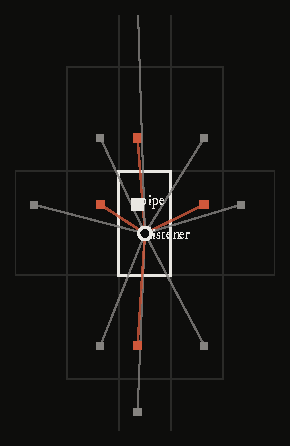
\includegraphics[width=\linewidth]{figs/image_sources.pdf}
  \caption{Image sources up to order 2.}
  \label{fig:images}
\end{subfigure}\hfill
\begin{subfigure}[b]{0.55\linewidth}\centering
  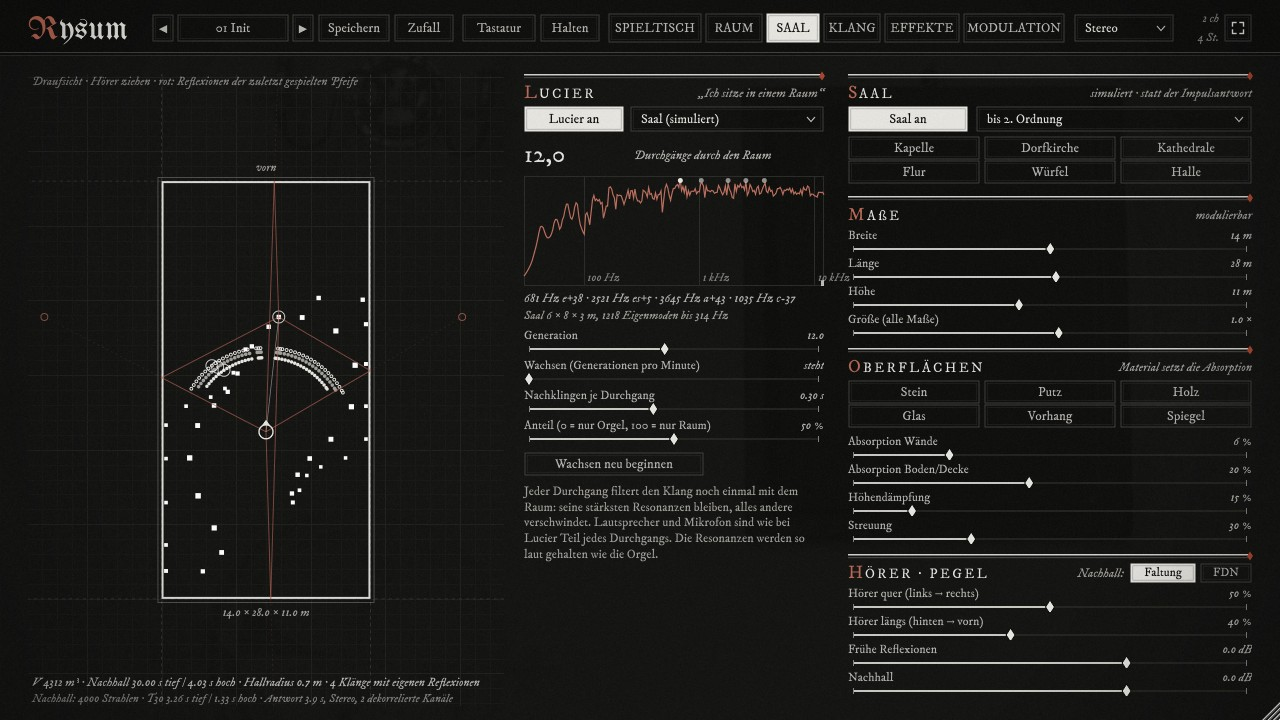
\includegraphics[width=\linewidth]{screens/ui_saal.jpg}
  \caption{The \ui{Saal} page.}
\end{subfigure}
\caption{The simulated room. (a) Top view of a $14\times\SI{28}{m}$ room with the mirrored rooms; red:
first-order images and their paths to the listener, grey: second order. (b) In the interface the plan
shows the pipes of the pulled stops and, in red, the reflections of the last pipe played.}
\end{figure}

\paragraph{Late reverb by ray tracing and synthesis.} The late reverberation follows the approach of
room-acoustics software such as RAVEN \citep{schroeder2011raven}. A ray tracer
\citep{krokstad1968} sends 4000 rays with specular and diffuse (Lambert) reflections and air absorption
through the room and derives an energy decay per band (least-squares fit between \SI{-5}{dB} and
\SI{-35}{dB} of the backward-integrated curve). Ray tracing matters when absorption is uneven or the room is
not diffuse: a corridor with hard walls and a dead floor rings far longer than Eyring's formula
\citep{eyring1930} predicts (\S\ref{sec:verification}). From the decay, a dense noise response is
synthesised -- one independent noise per Ambisonics channel up to second order (two for stereo), with the
energy of a diffuse field, in two bands with their own decay -- and convolved with the organ. A noise
response has no modes, so it cannot ring. The reverberant level follows the room's critical distance,
softly capped at \SI{+4}{dB}, so that large damped rooms sound drier and small hard ones wetter.

The convolution is non-uniformly partitioned (256/2048/8192 samples, after \citet{gardner1995}; \S\ref{sec:perf}) and keeps
its input history independent of the impulse response. When the room changes -- also continuously, under
modulation -- a new response is built in the background (about four times per second while the room keeps
changing) and the output is crossfaded between two convolutions of the \emph{same} input history, so the
reverb that is already sounding turns into the new room's without a gap. The noise is generated with a
fixed seed per channel, so successive responses differ only in their envelopes and held tones do not jump
in level.

\paragraph{Ringing out.} A long room used to be cut off: responses were at most \SI{6}{s} long and faded with a cosine from \SI{-30}{dB}, so a
cathedral stopped audibly instead of dying away. A response is now made long enough for the room to fall by \SI{75}{dB}, up to \SI{12}{s}; a
room that rings longer still has its decay bent down smoothly near the end, by an extra loss that grows quadratically from 35\,\% of the length, instead
of a fade. A room that no source plays into any more keeps ringing at its level with a silent input (the gain used to sit on the input and was ramped
to zero, which cut the tail), the host is told the real tail length instead of a fixed \SI{2}{s}, so stopping or bouncing does not cut a long room, and
a loaded impulse response that is cut at \SI{10}{s} gets a smooth fade of \SI{2}{s} instead of \SI{50}{ms}. In the render test a room with a reverberation time of \SI{30}{s} in the low band
and \SI{9.2}{s} in the high band, far longer than the \SI{12.1}{s} response can hold at its natural decay, falls by at most \SI{1.6}{dB} per \SI{50}{ms} and stands at \SI{-76.9}{dB} \SI{0.15}{s} before the
end of the response. A second check looks for unwanted dispersion in the Saal: a click sent through it arrives in all bands at once, and only the
ice walls (below) are seen by the measure, as they should be.

\paragraph{Feedback delay network.} Alternatively the late reverb can be a feedback delay network
\citep{jot1991fdn}: 16 delay lines around the room's mean free path, a random orthogonal mixing matrix
(a Hadamard matrix left isolated modes around \SIrange{1.5}{2}{kHz}), slow modulation of every delay line
($\pm8$ samples at different rates), two-band decay per line from the same ray tracing, and the lines spread
over 16 directions. It sounds slightly more alive and grainy and costs less CPU. When switching between the
two while playing, the previous tail rings out underneath.

\paragraph{Ice walls (\ui{Eis}).} On frozen lakes a shot or a falling stone comes back as a descending
\enquote{pew}: the ice disperses, and the low frequencies travel more slowly than the high ones. \ui{Eis} (below
\ui{Nachhall}) gives every early reflection this dispersion. The reflections are collected on their own buses, the
first-order ones (16 channels) and the higher-order ones (4 channels), and each channel passes through a cascade of
first-order all-passes
\begin{equation}
  H(z)=\left(\frac{a+z^{-1}}{1+a\,z^{-1}}\right)^{\!K},\qquad a=-\bigl(0.55+0.4\,\ell\bigr),
\end{equation}
with $K=64$ stages for the first-order and $K=96$ for the later reflections (their longer paths disperse more) and
$\ell$ = \ui{Eis Länge} (a chirp of roughly 5--50\,ms). With $a<0$ the group delay is largest at low frequencies, so
every reflection becomes a falling chirp from its own direction. \ui{Eis} crossfades from the plain reflections to only the
chirps. The late reverb is not affected.

\subsection{Flexible room geometry (\ui{Grundriss})}
\label{sec:plans}
The first version of the \ui{Saal} could only be a shoebox. The room now has a \emph{floor plan}, a polygon with
vertical walls, flat floor and flat ceiling; the height is independent of it. The nine plans
(Figure~\ref{fig:plans}; chosen by the row of small pictures above the plan) are:
\ui{Quader} (the shoebox, the default and exactly as before), \ui{L-Form} (a corner missing, so that reflections
go round the corner and some paths are hidden), \ui{Fächer} (narrow at the organ, wide at the back),
\ui{Sechseck}, \ui{Achteck} (a central building), \ui{Rund} (twelve walls on a superellipse; concave, so it
focuses the sound), \ui{Kreuz} (a nave with a transept), \ui{Apsis} (a nave ending in a round apse) and
\ui{Gezeichnet} (the user's own plan). A control \ui{Form (Grundriss)}, $a\in[0,1]$, sets how far the plan
departs from the rectangle (the width of the missing corner, the narrowing of the fan, the depth of the
apse and so on) and is a modulation target: the room can change shape while one plays. Width and length are the
bounding box of the plan, and the plan is stored in unit coordinates scaled by them. At most twelve corners are
possible (\fn{kMaxPlanVerts}).

\begin{figure}[t]
\centering
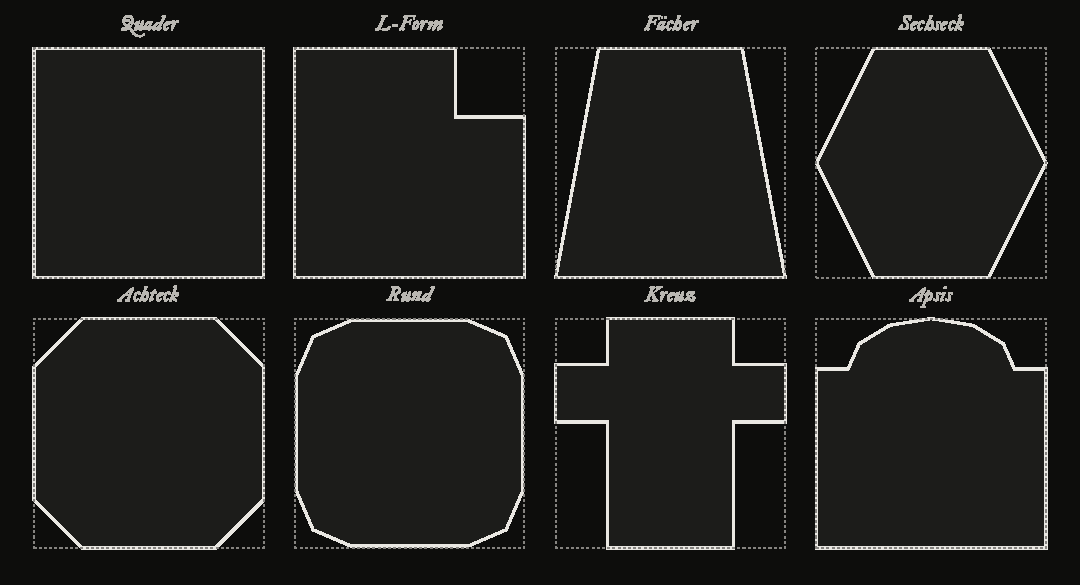
\includegraphics[width=0.85\linewidth]{figs/floorplans.pdf}
\caption{The eight preset floor plans at $a=0.5$ (vertex rules taken from \fn{makeFloorPlan}; dotted: the bounding
box given by width and length). The ninth plan is drawn by the user.}
\label{fig:plans}
\end{figure}

\paragraph{Drawn plans.} A drawn plan has 3 to 12 corners: they are dragged in the plan, a double click on a
wall inserts a corner, a right click removes it. A plan whose walls would cross is refused, and a clockwise polygon is
reversed so that the inward normals are consistent. A right click offers to start from the shape that is currently seen.
The drawn plan is saved with the project and in patches.

\paragraph{Image sources in a polygon.} For a polygon the mirror images are found by reflecting the source over
every \emph{sequence} of walls up to the chosen order, and only paths that really hit the walls are kept: the
reflection point of every leg must lie on the wall segment and not only on the line through it. In
non-convex plans (\ui{L-Form}, \ui{Kreuz}, \ui{Apsis}, drawn plans) a path is dropped if another wall blocks one of its legs
(\fn{planBlocked}). Floor and ceiling images are combined with the wall images as in the shoebox, and the
62 nearest images are played, as before. Each wall is stored with an inward unit normal, so reflecting a point is
$\mathbf p'=\mathbf p-2\,d(\mathbf p)\,\mathbf n$ with $d$ the signed distance. Since this search is expensive, it
runs only when a pipe has moved about \SI{12}{cm}, the room changed or a sound starts, and it is spread so that
every sound searches at most once in six blocks; in between the known paths simply move with the pipe. Paths
that appear or vanish (a reflection sliding past the end of a wall) fade in and out over \SI{25}{ms}, so nothing
clicks.

\paragraph{Late reverb and Lucier.} The ray tracer of the late reverb follows the same walls, so the decay
belongs to the plan. Pipes and the listener are kept inside the plan: a pipe stops
\SI{0.3}{m} before the wall along its line to the listener, so its direct sound always reaches the listener. The room modes
of the Lucier mode (\S\ref{sec:lucier}) still use a shoebox of the same floor area: the exact modes of an
arbitrary plan would need a wave solver.

\paragraph{Cost.} The cost is about that of the shoebox; in non-convex plans the worst case (48 moving pipes at
third order) is about 10--20\,\% higher.

\paragraph{Four rooms.} Every stop and the audio input can sound in one of four rooms, \ui{Saal 1--4} (a click on
the stop's number in the row \ui{im Saal} chooses the next room, a right click selects one). Each room has its
own size, plan, surfaces and listener position; the reflection order and the two levels are shared. Each room in
use gets its own early reflections and its own late reverb, built in the background like the first, so the cost
grows with the number of rooms in use. Clicks, the user's own sounds and effects stay in room~1, and everything
starts in room~1, so that older projects sound as before. The patches \ui{83 Vier Räume} and \ui{85 Nah und fern}
use this (Appendix~\ref{app:patches}). Like the plans, this part was written after the verification run of 1~November; the run of
15~November checks that \SIrange{1.5}{3.5}{s} after its key is let go the Praestant has died away in a small room~1 but still rings when the stop
is put in a cathedral as room~2.

\paragraph{Single surfaces.}\label{sec:surfaces} Floor, ceiling and each wall of a plan can be of a material of its own (\ui{Stein},
\ui{Putz}, \ui{Holz}, \ui{Glas}, \ui{Vorhang}, \ui{Spiegel}). On the \ui{Saal} page the surface is chosen next to \ui{Oberflächen} and a material
pressed (pressed again: back to the sliders); in the 3D view one looks at a surface and presses \textbf{M}. A surface without a material
follows the sliders. One with a material reflects with the absorption of that material, damps the highs, feeds the ray-traced reverb with
it (\S\ref{sec:plans}) and is drawn in its look; the choice is saved with the project. Per surface the absorption is split into the two bands of
the room: for the material's absorption $a$ and its damping of the highs $h$ the low band is $a$ and the high band
$a + 0.6\,h\,(1-a)$, both limited to $0.99$.

\paragraph{Out of sight.} In a plan that is not convex (L, cross, apse, \dots) a wall can stand between the listener and a
pipe. This happens when the listener walks (\ui{Hörer} on the living-organ tab, or the 3D view) and when the pipe
flies through the room (\S\ref{sec:roommotion}). The direct sound then does not come through the wall but around the
corner. The plan's \emph{reflex} corners are moved \SI{5}{cm} into the room (\fn{planCorners}); the shortest path
from the listener over one corner, or over two (into the far arm of a cross), is found, and the pipe is heard from the direction
of the first corner, over the whole longer way. The sharper the way bends, the quieter and duller it is: with the
total bend $\beta$ at the corners and $b = \beta/\pi$ the loss is $20\,b$\,dB (\SI{10}{dB} round a right angle) and the
low-pass cutoff $20\,\mathrm{kHz}/(1+40\,b)$ (about \SI{1}{kHz} round a right angle). At the edge of the shadow the bend is zero,
so nothing jumps as one steps past the corner. If no way is found (a strange plan) the straight line through the wall is
used, \SI{30}{dB} down and low-passed at \SI{500}{Hz}. Only the direct sound is treated like this; the reflections still
arrive from where they reach the listener. The 3D view shows how many sounding pipes are heard around a corner.

% =====================================================================
\subsection{Lucier mode}
\label{sec:lucier}
Alvin Lucier's \enquote{I am sitting in a room} (1969) plays a recording into a room and records it again,
over and over; after a few dozen generations only the room's resonances remain. The Lucier mode applies this
process to the whole output in real time. Generation $n$ is the sound convolved $n$ times with the room's
impulse response $h$; in the frequency domain this is $H^n$, so every resonance is multiplied once more and
rises above its surroundings.

The room is either the simulated hall of \S\ref{sec:room} or an impulse response loaded on the \ui{Raum}
page. For the simulated hall the eigenmodes of the shoebox are summed up to a crossover frequency $f_c$
(between \SI{60}{Hz} and \SI{400}{Hz}, lowered until at most 4000 modes are summed); above $1.25\,f_c$ the
response is a diffuse field whose two bands decay with the Eyring times, and the two parts are blended
between $0.8\,f_c$ and $1.25\,f_c$. Each pass also contains the loudspeaker and the microphone, modelled as a
second-order high-pass at \SI{60}{Hz} and a first-order low-pass at \SI{10}{kHz}:
\begin{equation}
  T(f) = \frac{(f/\SI{60}{Hz})^2}{\sqrt{1+(f/\SI{60}{Hz})^4}}\cdot\frac{1}{\sqrt{1+(f/\SI{10}{kHz})^2}} .
\end{equation}
One pass $H(f)=T(f)\,R(f)$ is normalised to unit rms level between \SI{60}{Hz} and \SI{10}{kHz}.

Real passes last the whole recording. To hear the resonances within seconds, every pass is damped by an
exponential window with time constant $\tau_{\mathrm{eff}}=\min\bigl(\tau,\;2.5\,\mathrm{s}/(n-1)\bigr)$, where
$\tau$ is the \ui{Nachklingen} setting (default \SI{0.3}{s}). The response of $n$ passes is
\begin{equation}
  G(f) = g\,|H(f)|^{n}\,e^{\,\mathrm{i}\,n\arg H(f)},\qquad g=\frac{1}{\sqrt{p\,r}},
\end{equation}
where $p$ is the peak and $r$ the rms magnitude of $|G|$ in the audible band. The factor $g$ keeps the
resonance from exploding while the rest of the spectrum does not vanish. Fractional generations blend
linearly between the two neighbouring whole passes. The response is computed on a background thread and
crossfaded in whenever the generation, the room or the damping changes.

The \ui{Anteil} setting $m\in[0,1]$ mixes the organ and the room with equal power, $\cos(m\pi/2)$ for the
dry and $\sin(m\pi/2)$ for the wet signal. Because the narrow resonances may or may not be hit by the organ's
partials, the wet level is controlled automatically, as in Lucier's own re-recording: the gain follows
$\sqrt{E_{\mathrm{in}}/E_{\mathrm{out}}}$ (energy envelopes, clamped to $[0.25,100]$), falls with a time
constant of \SI{30}{ms} so that a chord hitting a resonance is caught at once, and rises with \SI{1.5}{s}.
In silence the gain holds and the room rings out naturally.

\ui{Wachsen} raises the generation by itself, by up to 20 generations per minute, to at most 40. The
display shows the response between \SI{30}{Hz} and \SI{12}{kHz} in decibels and its five strongest resonances
(local maxima at least a sixth of an octave apart), each with its nearest note from $a'=\SI{444.5}{Hz}$. An
impulse response can be loaded instead of the simulated hall; it is normalised in the same way.
Patches 59--63 demonstrate the mode.

\subsection{Lucier's piece (\ui{Stück})}
\label{sec:lucierpiece}
Besides the live mode the Lucier controls offer the piece as it is performed. A recording is made
(\ui{Aufnehmen}; a voice, the organ, anything that is audible in the plug-in, or only the audio input,
at most five minutes) or loaded from a file. The recording is played, then generation 1 -- the recording
played into the room and recorded again --, then generation 2 and so on, each as long as the recording, until
the set number of generations is reached (for one minute and 32 generations about 33 minutes).

Every generation is one real pass through the room: the whole previous generation is convolved with the
room's response, undamped and with the full reverberation and with loudspeaker and microphone included, and
brought back to the level of the recording (RMS, never above $-\SI{1}{dBFS}$), as Lucier re-recorded every
generation at full level. The next generation is computed on a background thread while the current one
plays (about one second per minute of recording on the author's computer). The audio thread keeps two
playback slots, plays one and reads the other once it is marked as filled; buffers that the audio thread
may still read are freed one second later. Between generations a pause can be set, and a control
sets the share of the live sound against the playback (equal power) while the piece runs. The playback
is mono and leaves the plug-in in the middle (the $W$ channel in Ambisonics). Recordings are saved in
a folder of the user and remembered by the project; \ui{Stück als WAV} renders the whole piece into one
file in the background, faster than real time.

\emph{Status:} the piece mode, like the loudspeaker decoder, was added after the verification run of 1~November and is
described from the source code. The render test of 15~November checks that one pass is the convolution with the room (an impulse through one
pass differs from it by \SI{-140}{dB}), that every generation brings out more of the resonances (contrast 5, 17, 58 and \SI{82}{dB} at generations
0, 1, 4 and 12), that the level is held without clipping, and that twelve generations of \SI{10}{s} are computed in about \SI{3}{s}.

% =====================================================================
\section{The Saal in 3D (\ui{Begehen})}
\label{sec:walk}
% =====================================================================

The button \ui{3D begehen} on the floor plan of the \ui{Saal} page opens a page that shows the room in three dimensions,
seen through the listener's eyes (\fn{Walk3D.*}, \fn{WalkView.*}; Figure~\ref{fig:walk}). The pipes float where Ambisonics places them, with their
motion and modulation; sounding pipes glow. What began as a way to look at the Saal has become a second way to play the instrument:
the pipes are bodies that the player knocks, carries, throws, pins, arranges and blows about (\S\ref{sec:hands}), the room can be made
larger, darker or another material while one walks in it, a set of \emph{illusions} bends what is heard against what is seen
(\S\ref{sec:illusions}), and an audience can join in with their phones (\S\ref{sec:audience}). Everything in this section was written after the
verification run of 1~November; what the test run of 15~November covers is listed in \S\ref{sec:verification}.

\begin{figure}[!htb]
\centering
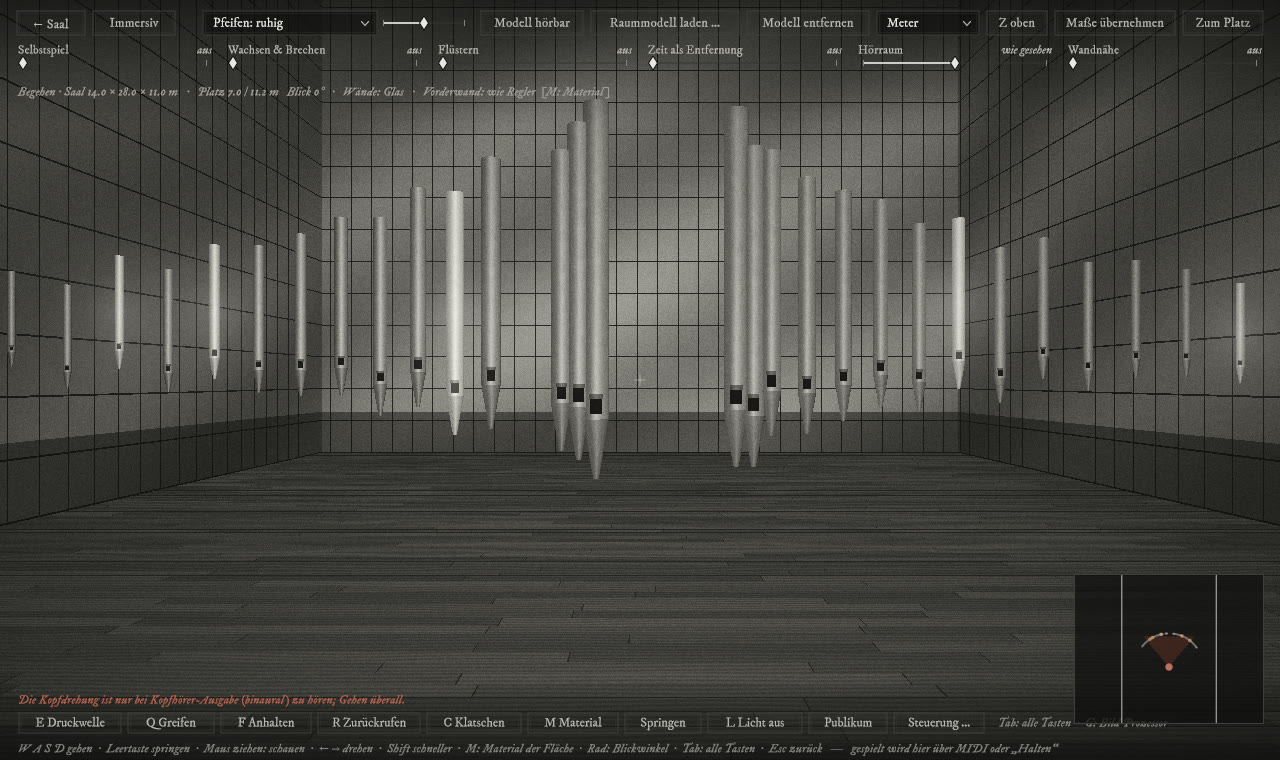
\includegraphics[width=\linewidth]{screens/ui_begehen.jpg}
\caption{The page \ui{Begehen}. Top: back to the \ui{Saal}, \ui{Immersiv}, the player's force (\ui{Pfeifen: \dots}), the room model,
and below the six sliders of the illusions. Middle: the Saal seen from the listening place, the sounding pipes glowing; the cross in
the middle aims. Bottom: the hands as buttons (\ui{E Druckwelle} \dots\ \ui{Publikum}, \ui{Steuerung \dots}), a line of hints and the
map, which turns with the view.}
\label{fig:walk}
\end{figure}

\subsection{Walking}
The keys \textbf{W A S D} walk, dragging the mouse looks around, the left and right arrow keys turn, \textbf{Shift} runs,
\textbf{Space} jumps, the mouse wheel changes the field of view and \textbf{Esc} goes back; holding \textbf{Tab} shows every key of the view
(Figure~\ref{fig:walkkeys}). The camera \emph{is} the listener: walking moves the listener of the room simulation and of the direct sound (the
same offset as \ui{Hörer}, \S\ref{sec:live}, with a quicker glide of \SI{40}{ms}) and the walls stop one. The turn of the head is heard on
headphones (binaural, transaural) and, since 15 November, on the AmbiX outputs as well: the whole field that is sent out (orders 1--5, the room
included) is turned about the vertical axis by the view's yaw, gliding within the block, and glides back to the front when the view closes; a host bus
with fewer channels than the order is turned in the orders it carries. Both use the same rotation (\fn{AmbiYawRotator}), so headphones and AmbiX turn
alike; in the test the direction of a held chord, read from the first-order intensity, turns by \SI{-90.0}{\degree} when the head turns \SI{90}{\degree}
to the left. With loudspeaker outputs the field stays where it is, since the room around the loudspeakers does not turn with the head. While the view holds the keyboard the
walking keys do not play notes; one plays over MIDI, or holds a chord with \ui{Halten}. A small map at the bottom right turns with the view.
Walking is smooth: the speed builds up and dies away (after \SI{0.1}{s} one has gone \SI{6}{cm}, after a second \SI{1.4}{m}, and one coasts
on about a quarter of a metre), the view follows the mouse within a few hundredths of a second, a jump rises about \SI{0.8}{m} and lands after
\SI{0.7}{s} (the ears go up with it), and steps of up to \SI{45}{cm} are climbed.

\paragraph{Immersive view.} \ui{Immersiv} (button or \textbf{I}) leaves nothing but the picture: the window goes to full screen and comes back
afterwards, buttons, writing and map disappear, and only the small cross in the middle stays. The mouse looks around without a button
held: the pointer is hidden and kept inside the view. A click knocks on the pipe under the cross, and all the hands below act at the cross.
\textbf{Esc} or \textbf{I} goes back, and so does switching to another program, which also frees the pointer at once. Pressed from another page
(for instance by a MIDI button) it does nothing.

\paragraph{Controls of this computer.} \ui{Steuerung \dots} sets how fast the mouse looks around ($\times0.25$ to $\times3$), a mouse upside down
(up looks down) and the walking pace (\ui{Gehtempo}, $\times0.4$ to $\times8$, also \textbf{Shift+wheel}; the menu offers $\times0.5$ to $\times2$, \ui{rasend}
$\times3.5$ and \ui{wie der Wind} $\times6$). Running with \textbf{Shift} is about 2.6 times the walking speed, so at $\times6$ one runs at about
\SI{25}{m/s} and at $\times8$ at about \SI{34}{m/s}. The walls still stop one at these speeds, since a step is tested along its whole way. In a shaped room
(\S\ref{sec:plans}) the listener's place used to follow at most \SI{6}{m/s}, so a sprint left its own sound behind; it now follows up to \SI{40}{m/s}.
These settings belong to the computer and the hands of its player, not to the music: they are kept in \fn{Documents/Rysum/Steuerung.xml}, not in the project.

\subsection{Room models}
\label{sec:models}
\ui{Raummodell laden \dots} takes an OBJ file (vertices, faces with any index form, negative indices and polygons, and the
colours of an MTL file, up to 80\,000 triangles) as the room that is shown; \ui{Meter / Zentimeter / \dots} and \ui{Z oben} fix the
units and the vertical axis of the import, and \ui{Maße übernehmen} gives the Saal the width, length and height of the
model (as a rectangle). The model is seen and walked: its walls stop one and its floors carry one (\fn{MeshAcoustics.h}). With \ui{Modell hörbar} it is also
\emph{heard}, as described below. The Saal's shoebox stays underneath (it is no longer drawn): it gives the early
reflections, closes a model that is open somewhere, and its floor and ceiling are drawn far beyond the model, so a model without
a floor or a roof never shows a black void. \ui{Zum Platz} goes back to the listening place. The file and the place where one stands are saved with the project, not with the
patches (except the built-in rooms, below); a missing file is kept by name.

\paragraph{Hearing the model.} The triangles of the model (corner, two edges and a unit normal each; level faces low down are
floor, level faces high up ceiling, the rest walls) are placed in a tree of bounding boxes when the model is loaded, so that a ray finds
what it hits in a few steps; casting a ray allocates nothing and is safe on the audio thread. Two things use it.
\begin{itemize}
  \item \emph{Line of sight.} A pipe behind a wall or a pillar of the model is heard around its edge. Rings of growing angle are
        searched around the line from listener to pipe; the first ring with a way through decides, which is the way with the
        smallest bend and therefore the shortest and loudest one, and the sound comes from the direction of that bend with
        the whole length of the detour. Loss and cutoff grow with the bend as in the floor plans, so that nothing jumps at the edge of
        the shadow. If there is no way with one bend, the sound goes through the walls: with $n$ surfaces crossed
        (at most 6 are counted; a wall has two) the loss is $\min(36,\,9n)$\,dB and the cutoff $\max(250,\,1600/n)$\,Hz.
  \item \emph{Late reverb.} Rays are traced through the model as in the Saal (\S\ref{sec:plans}), 1500 of them by default: they bounce
        off the model's triangles, its floors with the absorption of the Saal's floor, its ceilings with that of the ceiling and everything else
        with the mean of the Saal's walls, mirror-like or scattered as in the Saal. A ray that finds no triangle (a model that is open at the top,
        a doorway) meets the shoebox, so none is lost and an open model still has the size of the Saal; the shoebox is grown to hold the
        whole model.
\end{itemize}
The decay of a big model therefore is that of its own geometry, not of a rectangle of the same size.

\paragraph{Pipes in the model.} The bodies of the room motions (\S\ref{sec:roommotion}) collide with the model too: with its walls, columns,
steps and floors. A box query on the tree says when a pipe is near a surface at all; only then rays along the step, cast from several points on
the pipe's axis, find the surface it would pass through. The pipe bounces off it with the coefficient of its motion, lands and rests on a floor
of the model (a gallery, a step, a landing) and knocks where it hits (\S\ref{sec:roommotion}). A pipe that starts inside a solid passes through until
it is out, so a model loaded around flying pipes does not trap them.

\paragraph{Built-in rooms.} Six rooms come with the plug-in, in the menu of \ui{Raummodell laden \dots}; they are made in code
(\fn{RoomModels.cpp}) and written as ordinary OBJ files with a shared MTL into \fn{Documents/Rysum/Modelle} when chosen, so they can also be
opened elsewhere:
\begin{center}\small
\begin{tabularx}{\linewidth}{@{}llX@{}}
\toprule
Room & Size (m) & What is in it \\
\midrule
\ui{Kapelle}      & $12\times24\times9$  & columns, pews, altar steps \\
\ui{Hallenkirche} & $21\times40\times15$ & three aisles, a west gallery reached by a stair \\
\ui{Krypta}       & $13\times17\times4$  & sixteen short columns under ribs \\
\ui{Rotunde}      & 18 round, 15 high    & a ring of eight columns under a dome \\
\ui{Kreuzgang}    & $25\times25\times9$  & a covered walk around an open court with a well \\
\ui{Treppenturm}  & $9\times9\times23$   & five flights of twenty steps up to a landing \SI{20}{m} above the floor \\
\bottomrule
\end{tabularx}
\end{center}
They have between 724 and 1466 triangles. They are closed (except the court), their walls have a thickness, and their steps are
\SIrange{18}{20}{cm}, so that everything meant to be climbed can be climbed. Choosing one loads it z-up in metres, gives the Saal its size and puts
the listener at a free place in it. A patch saved in a built-in room keeps that room and the light (\S\ref{sec:architecture}); the factory set~17
(Appendix~\ref{app:patches}) uses this for twelve of its sixteen patches.

\subsection{The picture}
\label{sec:walkgpu}
The room is drawn in greys like an old print, with moving film grain. Its surfaces follow the acoustics of the Saal:
the wall absorption, high damping and scattering pick the nearest of the Saal page's materials (\ui{Stein}: ashlar blocks,
\ui{Putz}: plaster, \ui{Holz}: panelling, \ui{Glas}: leaded panes, \ui{Vorhang}: heavy folds, \ui{Spiegel}: bright and smooth);
the more a surface swallows, the darker it is, scattering makes it rougher and high damping duller. Floor and ceiling follow
their own absorption (stone slabs, boards, carpet). The pipes look like what they are, with the sizes of \S\ref{sec:roommotion} and the
mouth turned towards the listener's place: the flue pipes of tin with a conical foot (to 16\,\% of the length) and a round body; the Gedackt as
square wooden pipes with a mouth cut into the front and a stopper on top; the Trompete as reed pipes, a round boot below and a long funnel
widening to its open top. The knock follows the material: on the wooden Gedackt it is dull and short with a dry \enquote{tock} (in the render
test the wood's highs are \SI{18}{dB} and its tail \SI{43}{dB} below those of tin).

\paragraph{Light off.} \textbf{L} (or the button \ui{L Licht aus}) turns the light off (Figure~\ref{fig:walkrooms}b). With nothing sounding the room can
barely be made out: the rest of the usual light is 1.8\,\%, the silent pipes keep only a ghost of an outline, and the film grain is halved so
that nothing glitters where no lamp shines. The sounding pipes light the room, each a small lamp, brighter the louder it sounds and the more wind it
gets (since 17 November a pipe's light follows its actual wind -- the stop's draw, the shared bellows, its pallet, \S\ref{sec:live} --, which the
engine publishes per pipe next to the mask of sounding pipes; the glows in the 3D view, the Saal plan and the sounding rings of the \ui{Raum} view
all use it, so a starved stop glows dimly), lighting
what faces it and fading with distance (there are no shadows); a knock flashes as a spark. A full chord is brighter than one pipe, but not without end.
In the test the mean brightness of the picture is 0.319 with the light on, 0.134 in the dark with a chord and 0.054 dark and silent.
\textbf{K} puts a \emph{lantern} where the cross points (a hand's breadth short of the surface, at least \SI{15}{cm} above the floor; up to 16):
in the dark each lights the room around it like a sounding pipe and shows a small flame (one lantern on the floor raised the mean brightness of a
silent dark room from 0.121 to 0.164). \textbf{Shift+K} takes the nearest away, \textbf{Ctrl+K} all of them. The light and the lanterns are saved with the project.

\paragraph{Rendering.} The renderer is a software rasteriser of its own: triangles are transformed, clipped and binned into bands of rows, which
are drawn on several threads at the full resolution of the screen; when a frame takes too long the view lowers its resolution by itself. Since
14~November the graphics card fills the pixels instead (\fn{WalkGpu.*}, OpenGL~3.2, which the built-in graphics of laptops of the last decade
also offer). The processor still places the room and the pipes, and the card draws the projected triangles with a shader that computes the
same formulas -- the patterns of the surfaces, fog, grain, the grey of the print and the lamps of the dark room -- and the glows of the sounding
pipes. Over the card's picture JUCE paints the writing and the controls, repainted only where they change; the processor keeps a depth map at
half size for what the cross points at and for the glows. A test mode draws the scene, each of the nine kinds of surface and a model both
ways: the mean difference between the two pictures is at most 0.012 of 255. With a full scene the whole program needs about a quarter of the
processor time it needed before, 0.7 instead of 2.6--3.1 cores including the sound (Ryzen~5 2600X with a Radeon RX~6700~XT, the only card it has
been measured on). \textbf{G} switches between card and processor (kept in \fn{Documents/Rysum/Grafik.xml}); if the context or the shader fails,
or while buttons are assigned to MIDI (\S\ref{sec:control}), the processor draws, as before. The sound does not use the card: its work is
thousands of small jobs that must each be done within about a millisecond, and the way to the card and back takes longer than the job.
The card draws into a native child window laid over the view. JUCE marks it click-through, but on one tester's computer Windows still counted it
as the window under the pointer, and it took every click: no button worked and only the walking keys, which are read directly, did anything. That
window is now disabled, which makes Windows pass its mouse input to the window below and never give it the keyboard (the fault could not be
reproduced on the development machine).

\paragraph{360-degree video.} \ui{360\textdegree{} Aufnahme} (next to \ui{Immersiv}) records what the view shows all around the eye,
together with the sound field, as the material for a 360-degree video with spatial sound such as YouTube plays it: the viewer turns the head
(or the phone, or drags the picture), and picture and sound turn together. A menu offers 2048, 2560, 3840 or 5760 pixels of width at 30 frames
per second (3840 also at 25). Into \fn{Documents/Rysum/360/}\emph{date and time} go the frames (\fn{frames/f\_000000.jpg} \dots, equirectangular,
the middle the Saal's front), \fn{ambix.wav} (first-order Ambisonics, AmbiX: W, Y, Z, X, 24 bit), a script \fn{make\_video.bat} (and \fn{.sh})
that puts them together with ffmpeg into \fn{rysum360.mov} (H.264 and 4 channels of PCM at 48\,kHz), and a \fn{README.txt} with the last step:
Google's Spatial Media Metadata Injector marks the file as a 360-degree video with AmbiX sound, and YouTube then plays it so. Both picture and
sound are fixed in the room, not in the player's head: the sound is taken before the head's turn and before the headphone or loudspeaker
decoder, so the output has to be Ambisonics of any order (AmbiX, headphones or loudspeakers; with a stereo output the button says so). The
player walks and looks around as usual; where the eye goes, the camera goes; where the player looks does not matter to the video. The ears
left behind with \textbf{H} take the camera with them.

Recording and drawing are two steps. While recording, the view keeps for every video frame that falls due the scene it has just
built -- its triangles in the room, the materials, the lamps and the glows -- and writes it to \fn{scene.bin} (the room's or model's
triangles only when they change; about 150\,kB per frame in the Saal with a chord). That costs almost nothing, so the recording keeps every
frame whatever the size of the video. After \ui{360\textdegree{} Aufnahme} is clicked again, a thread of its own draws every frame from
\fn{scene.bin}, with the processor, six times (a cube around the eye), resamples it into the panorama and writes the JPEG while the next one
is drawn; the button shows how far it is, and the folder opens when it is done. Drawing a 3840-wide frame takes about 0.27\,s on the
development machine (Ryzen~5 2600X), a 2048-wide one 0.11\,s: a minute of 4K video at 30 frames per second is drawn in about eight minutes.
The sound's clock decides which video frame a scene belongs to (\S\ref{sec:math-pano}); a frame for which the view gave no scene, because it
drew more slowly than the video's frame rate, repeats the one before, so picture and sound stay together. The recording has to be made in real
time, with the view open (not in a faster-than-real-time export of the DAW, which the view cannot follow).

\begin{figure}[!htb]
\centering
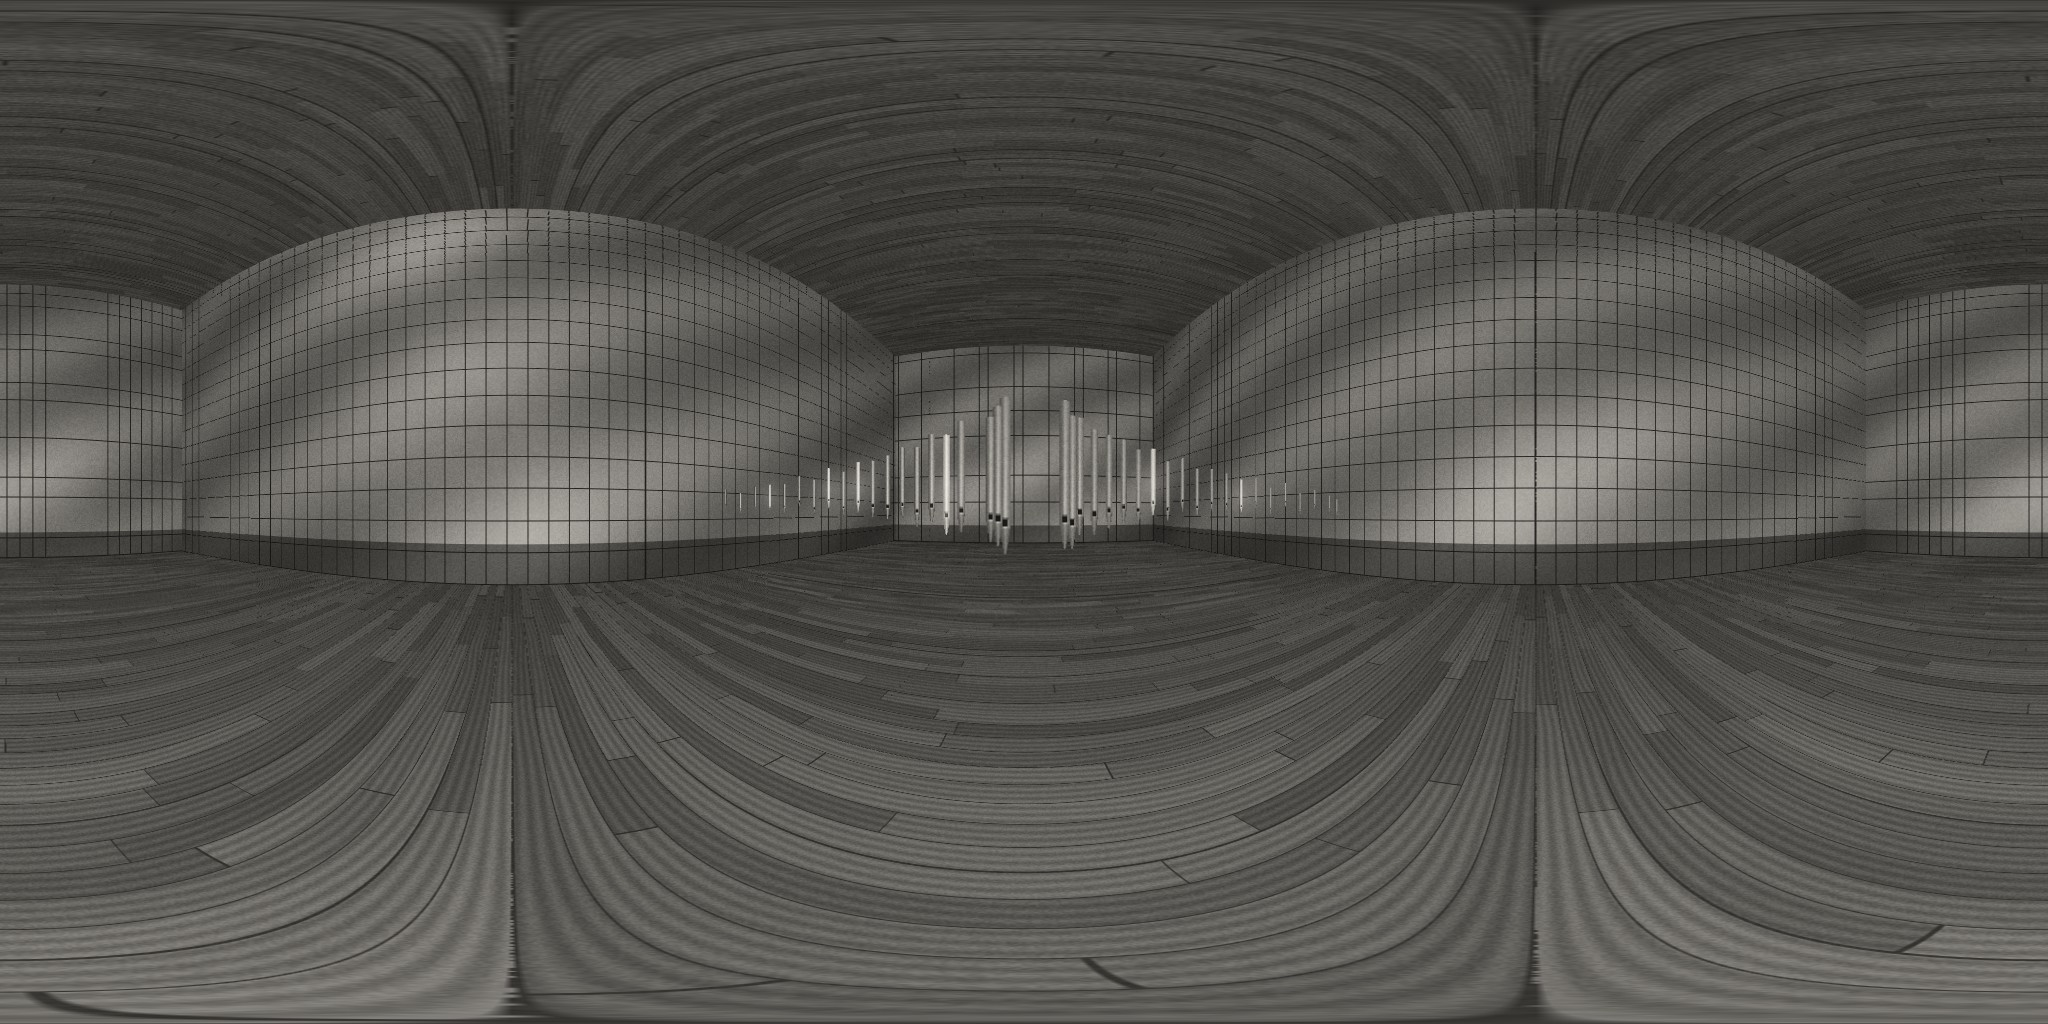
\includegraphics[width=\linewidth]{screens/walk360.jpg}
\caption{A frame of a 360-degree recording (2048\,$\times$\,1024, equirectangular): the Saal all around the eye, the middle its front with the
organ, the left and right walls at a quarter of the width from either edge, the back wall split at the edges, the ceiling above and the floor
below stretched over the whole width. A video player shows a part of it, turned as the viewer looks.}
\label{fig:walk360}
\end{figure}

\begin{figure}[t]
\centering
\begin{subfigure}[b]{0.495\linewidth}\centering
  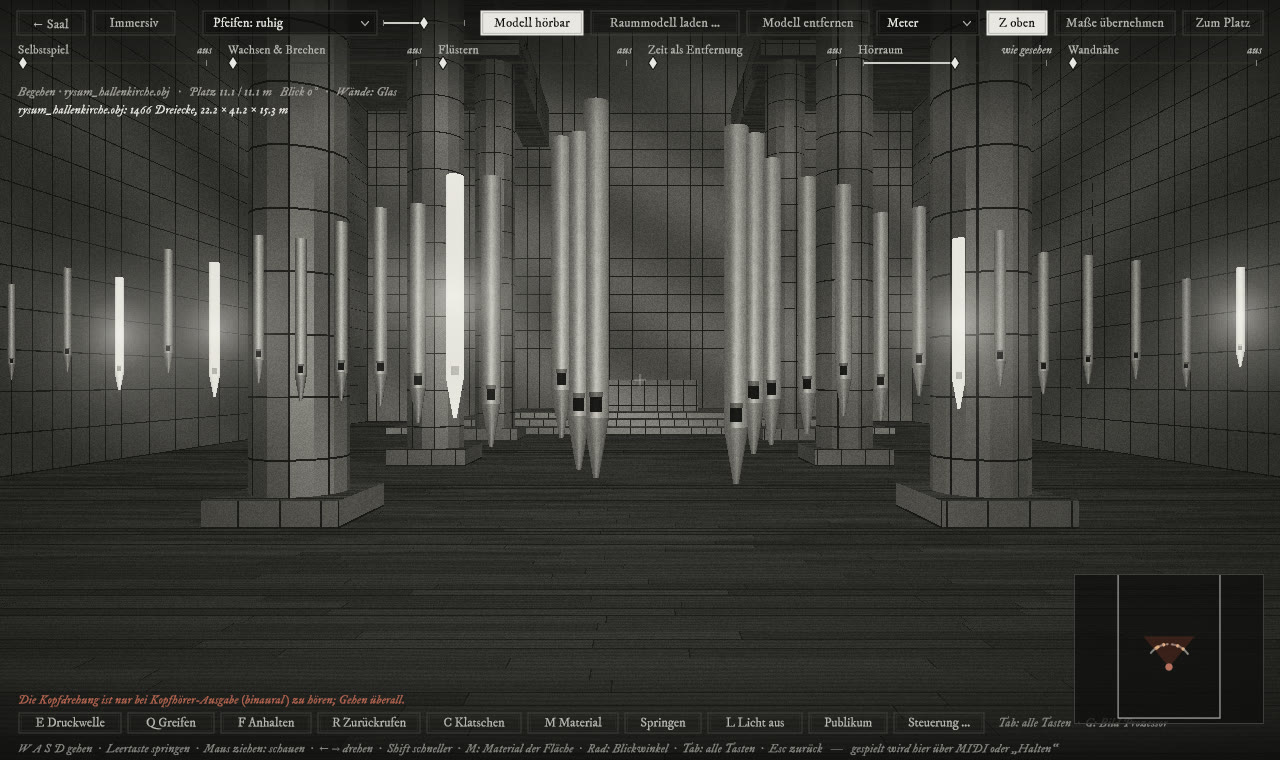
\includegraphics[width=\linewidth]{screens/ui_begehen_hallenkirche.jpg}
  \caption{\ui{Hallenkirche}}
\end{subfigure}\hfill
\begin{subfigure}[b]{0.495\linewidth}\centering
  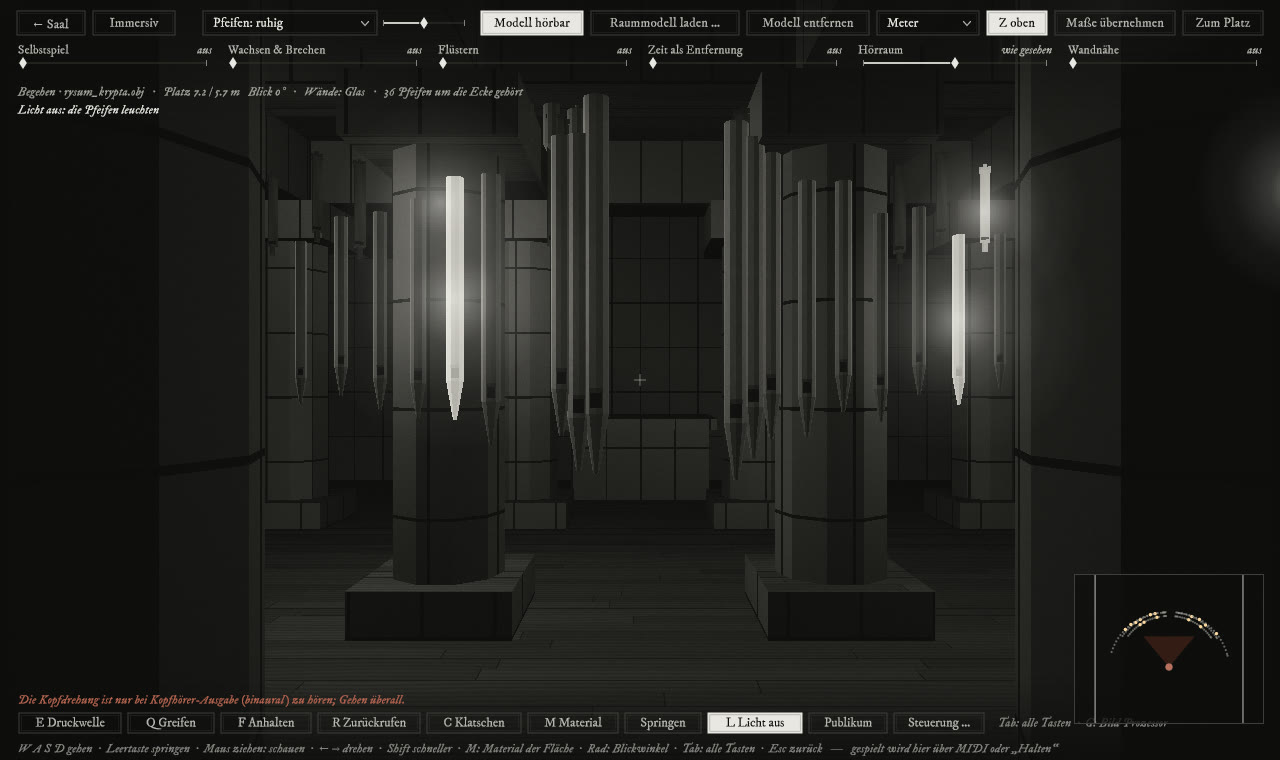
\includegraphics[width=\linewidth]{screens/ui_begehen_dunkel.jpg}
  \caption{\ui{Krypta}, light off}
\end{subfigure}
\caption{Two of the built-in rooms. (a) The hall church with the pipes floating between its columns. (b) The crypt with the
light off: only the sounding pipes light the columns and ribs; the line at the top says how many sounding pipes are heard around a corner.}
\label{fig:walkrooms}
\end{figure}

\subsection{The player's hands}
\label{sec:hands}
Since 13~November the keys of the view act on the pipes. They need the pipes to be bodies in the Saal (the room motions of
\S\ref{sec:roommotion}); a pulled stop that stands still is given the motion \ui{Schweben} by the first hand that needs it (the view says so),
while a stop with another motion (\ui{Rotation}, \ui{Pendel}, \dots) is left as it is. Pipes the player has just moved knock on the walls even when
\ui{Aufprall} is turned down. \textbf{Shift} makes every hand stronger (by 1.7). The view sends each act to the audio thread as a command
(\S\ref{sec:architecture}).
\begin{description}
  \item[E -- shockwave.] Every body within \SI{16}{m} of the listener is pushed away, the nearer the harder and a little upwards:
        with the strength $a$ and the distance $d$ the speed gained is
        \begin{equation}
          \Delta v = \frac{12\,a}{1+(d/\SI{6}{m})^2}\,\Bigl(1-\frac{d}{\SI{16}{m}}\Bigr)\ \text{m/s},
        \end{equation}
        along the line from the listener plus $0.3\,\Delta v$ upwards. It sounds as a deep thump falling from 112 to \SI{42}{Hz} within about a
        tenth of a second, with the air it moves, from everywhere and into the room. Held, the key repeats at most every \SI{0.3}{s}.
  \item[Q (held) -- carry and throw.] Takes the pipe under the cross (it gets a ring when one is within \SI{9}{m}) and carries it ahead of the
        eyes, between \SIrange{1.2}{3}{m} away; the mouse wheel brings it nearer (down to \SI{20}{cm}, to the ear, \S\ref{sec:illusions}) or further
        (\SI{4}{m}). The pipe follows the hand with a velocity that is steered towards $14\,(\mathbf h-\mathbf p)$ (at most \SI{25}{m/s}). Let go,
        it flies on with the hand's own speed, the player's walking speed and a push of \SI{4.5}{m/s} along the view (\SI{9}{m/s} with Shift);
        a hovering pipe glides, is slowed by the air and stays where it comes to rest.
  \item[F (held) -- hold still.] Everything that moves stops where it is, until the key is let go.
  \item[R -- call home.] Every pipe flies back to its place in the organ within three seconds, on a critically damped path (stiffness 9, damping
        6 per second), so it arrives without overshooting; grown and broken pipes (\S\ref{sec:illusions}) are mended.
  \item[C -- clap.] A hand clap where the listener stands, to hear the room from there: three contacts of the palms \SI{9}{ms} apart, then the hollow
        of the hands ringing out, noise through a band around \SI{1.2}{kHz}, \SI{0.3}{s} in all, sent strongly into the room.
  \item[Click -- knock.] A click on a pipe knocks on it like an impact of \SI{5}{m/s} (\SI{7.1}{m/s} with Shift; \S\ref{sec:roommotion}): it rings with its own
        bending modes and faintly its note, without its key, and gives way a little.
  \item[Click held -- bow.] Held still on a pipe for \SI{0.28}{s}, the click sounds it like a held key, wherever the pipe is now, until the button
        is let go.
  \item[Right button with Q -- set down.] With a pipe in the hand the right mouse button puts it where the cross meets the room (on the floor,
        against a wall, in the air), and there it stays.
  \item[Middle button -- pin.] A pinned pipe does not move: shockwaves, wind, magnet and whirlwind leave it where it is. A small nail head marks it;
        another middle click frees it.
  \item[T -- whirlwind.] For four seconds a whirlwind stands where the cross meets the room, but never more than \SI{5}{m} ahead (pointed at a far wall it
        would leave the pipes out). Within $r<\SI{7}{m}$ of its axis, with $c = 1-r/\SI{7}{m}$ and the strength $a$ fading out over the last
        \SI{1.5}{s}, a pipe's horizontal velocity is steered towards $6\,c\,a$ m/s around the axis, it is drawn in by $1.2\,c\,a$ and lifted by
        $2.5\,c^2 a$ m/s$^2$.
  \item[P -- pause, Z (held) -- slow motion.] \textbf{P} stops everything that moves until it is pressed again; holding \textbf{Z} lets the
        bodies' time run at a quarter (the whirlwind's too).
\end{description}
The hands are also buttons in a row at the bottom, so each can be put on a MIDI button (\S\ref{sec:control}); \ui{Greifen}, \ui{Anhalten} and
\ui{Springen} then act for as long as the MIDI button is held.

\paragraph{Arranging the pipes.} \textbf{Ctrl+click} chooses a pipe (again: out of the choice), \textbf{Ctrl+double-click} its whole stop,
\textbf{Ctrl+drag} a frame around several; \textbf{Esc} empties the choice, and red lozenges mark it (Figure~\ref{fig:walkarrange}a). The keys
\textbf{1 to 5} set the chosen pipes -- or, with none chosen, all pipes of the pulled stops -- in pitch order into a formation around where one stands,
at the height of the eyes less \SI{20}{cm}:
\begin{enumerate}
  \item a \emph{row} across the view, \SI{3}{m} ahead, the pipes \SI{0.42}{m} apart and the low notes on the left; more than 24 form rows \SI{0.8}{m} behind;
  \item a \emph{circle} of \SI{2.4}{m} radius, starting ahead and going right; every further 32 pipes a ring \SI{1.1}{m} wider;
  \item a \emph{spiral} as the seeds of a sunflower: pipe $i$ at the angle $2.39996\,i$ (the golden angle) and the radius $1.4+0.45\sqrt i$\,m, rising
        \SI{1.6}{m} from the first to the last;
  \item a square \emph{grid} ahead, from \SI{2.5}{m}, \SI{0.6}{m} apart;
  \item \emph{scattered} around, \SIrange{2}{7}{m} away and \SIrange{0.5}{3.3}{m} high.
\end{enumerate}
The pipes fly there on a critically damped path (stiffness 16, damping 8 per second, at most four seconds) and rest there. \textbf{Ctrl+F1 \dots\ F8}
keeps where the pipes stand now as a \emph{layout} (saved with the project, not with a patch), \textbf{F1 \dots\ F8} brings it back in one flight, and
\textbf{Ctrl+Z} undoes the last shockwave, throw, call home, whirlwind, formation, layout or magnet, up to 24 steps.
\textbf{Holding the right mouse button} is a \emph{magnet} a few metres ahead (the wheel moves it between \SIrange{0.8}{14}{m}): within \SI{14}{m}
each pipe is drawn to a distance of its own from the point (\SIrange{0.45}{1.35}{m}), so the pipes gather in a loose cloud rather than one point; with
Shift they flee from it (within \SI{10}{m}). Looking around meanwhile leads the cloud through the room, and the pipes stay where the magnet leaves them.
\textbf{Alt+drag} strokes over the pipes like a hand over strings: every pipe the pointer passes is knocked once, as hard as the pointer is fast.
In the immersive view all of this happens at the cross.

\paragraph{The room by hand.} \textbf{Ctrl+wheel} makes the Saal larger or smaller (its \ui{Größe}, 0.25 to 3 times; the reverb grows with it; not with a
model loaded, which has its own size); \textbf{Alt+M} gives every surface of the Saal the next material of the one under the cross (\textbf{M} alone: that
surface, \S\ref{sec:surfaces}); \textbf{H} leaves the ears where one stands: one walks on and watches while the engine still hears from there, a red ring
marking the place, until \textbf{H} again brings them back.

\begin{figure}[t]
\centering
\begin{subfigure}[b]{0.495\linewidth}\centering
  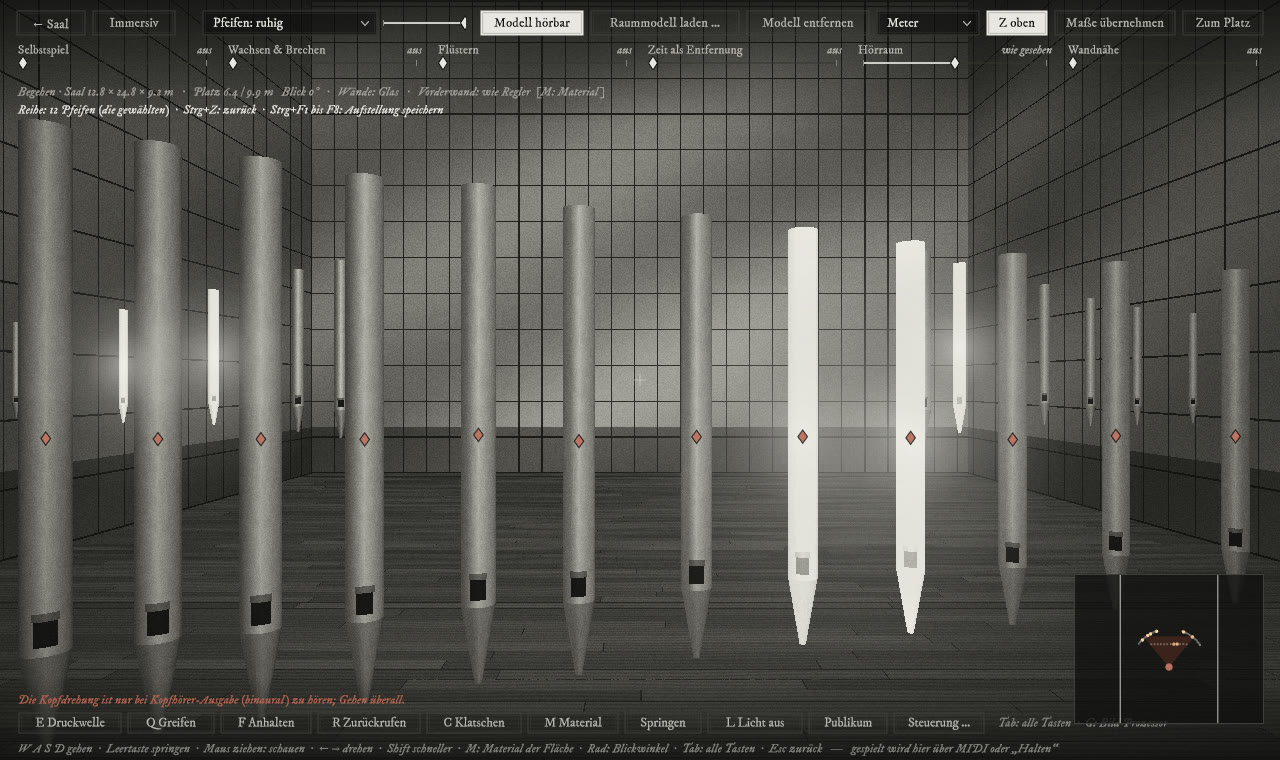
\includegraphics[width=\linewidth]{screens/ui_begehen_reihe.jpg}
  \caption{a row of twelve chosen pipes}
\end{subfigure}\hfill
\begin{subfigure}[b]{0.495\linewidth}\centering
  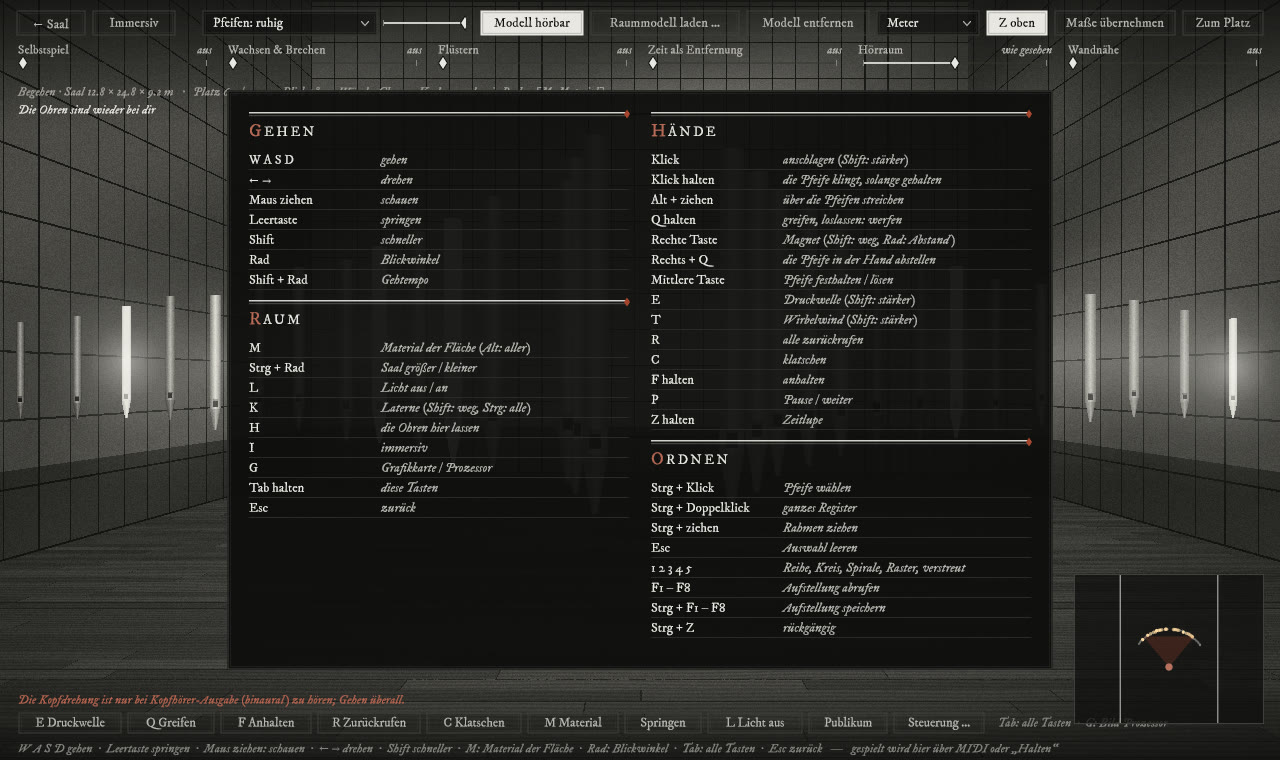
\includegraphics[width=\linewidth]{screens/ui_begehen_tasten.jpg}
  \caption{Tab held: every key}
\end{subfigure}
\caption{Arranging. (a) Twelve pipes chosen with Ctrl+click (red lozenges) and set into a row with the key 1, low notes on the left; the line at the top
names the formation and the keys to undo or keep it. (b) The keys of the view, in four groups: walking, hands, room, arranging.}
\label{fig:walkarrange}
\label{fig:walkkeys}
\end{figure}

\subsection{Illusions}
\label{sec:illusions}
A row of six sliders under the buttons (all off at first) bends what is heard against what is seen. All six are parameters, so they can be modulated,
automated and put on MIDI controllers.
\begin{description}
  \item[Selbstspiel] -- the room plays itself. A pipe of a pulled stop that knocks against a wall, the floor or the ceiling faster than \SI{0.5}{m/s} sounds
        its own note for $\min\bigl(5,\;0.12+s\,(0.25+0.4\,v)\bigr)$ seconds ($s$ the slider, $v$ the speed in m/s), so a harder knock gives a longer note;
        it needs stops whose motion takes place in the Saal, and nobody has to play. Never at the cost of what is played: such notes start only while
        at least eight voices are free, and at most 40 sound at once.
  \item[Wachsen \& Brechen] -- pipes that are not sounding slowly grow and sink: with the slider $g$ a pipe takes $600/(0.5+20g^2)$ seconds to
        double its length (half a minute at full strength, a quarter of an hour at 10\,\%), at most to twice, an octave down. A knock harder than
        $7-5g$\,m/s breaks a pipe in two: it is half as long and an octave higher (down to a quarter of its length), with a crack. The lengths are
        seen. One pipe stays one pipe: the broken-off half is heard as the crack, it does not fly on. Turned off, every pipe finds back within a few
        seconds; \textbf{R} mends them all at once.
  \item[Flüstern] -- a pipe within arm's reach of the head ($d<\SI{1.4}{m}$) is also heard at the two ears themselves, each by its own distance
        (the ears $\pm\SI{8.75}{cm}$ from the middle). With $t$ rising smoothly from 0 at \SI{1.4}{m} to 1 at \SI{0.2}{m}, the slider $w$ and the
        distances $d_e$ of the ear and $d_n$ of the nearer ear, an ear receives
        \begin{equation}
          g_e = 0.9\,w\,t\cdot\min\bigl(12,\;1/d_e\bigr)\cdot\bigl(d_n/d_e\bigr)^{0.7},
        \end{equation}
        the far ear later by the difference of the ways and low-passed at $\SI{18}{kHz}/\bigl(1+4\,(d_e/d_n-1)\bigr)$ (not below \SI{1.5}{kHz}), the
        head's shadow; the tone is warmer the nearer it comes. Because the room's own picture of the pipe and the ear signal would colour each other,
        the pipe leaves the room sound by the factor $1-0.85\,w\,t$ as it comes into the ears. The ear signals are added after the binaural decoding,
        so this works on headphones, over two loudspeakers and in stereo; with Ambisonics or loudspeaker output it does nothing. A carried pipe
        brought to the ear with the wheel is the way to hear it. In the render test a pipe \SI{15}{cm} from the left ear is \SI{16.6}{dB} louder there than
        at the right one.
  \item[Zeit als Entfernung] -- the front of the room plays the past. Everything that is heard runs through a memory of up to \SI{20}{s}
        (\fn{TimeDistance.h}; at most 12 million samples, so with many Ambisonics channels it is shorter, about \SI{14}{s} with third-order binaural at
        \SI{48}{kHz}), and it is read further back the further forward one stands: at the usual place the present, at the front wall as many seconds
        ago as the slider says. Walking forwards quickly, time is heard running backwards; walking back, it catches up. The reading speed is limited to
        twice backwards and four times forwards and changes smoothly within a hundredth of a second, since a sudden change of speed would be a kink in the
        sound. The top line says how far back one hears. It also follows the automatic walk of \ui{Hörer} (\S\ref{sec:live}).
  \item[Hörraum] -- the late reverb belongs to a room of another size than the one seen and walked in ($\times0.25$ to $\times8$; the traced decay is
        stretched with the size, also with a heard model): see a chapel, hear a cathedral. The early reflections stay those of the room one sees, and that
        contradiction is the illusion. Needs \ui{Saal an}.
  \item[Wandnähe] -- nearer than \SI{3}{m} to a wall the late reverb grows and gets louder, as if another room opened behind it: with $n = (1-d/\SI{3}{m})^2$
        and the slider $w$ the size is multiplied by $1+3wn$ and the level by $1+1.5wn$, smoothed over \SI{0.3}{s}; the reverb is rebuilt a few times a second
        as one walks and crossfaded (\S\ref{sec:room}).
\end{description}

\subsection{The audience (\ui{Publikum})}
\label{sec:audience}
The last button of the row lets an audience play along with their phones (Figure~\ref{fig:audience}). A QR code appears in the corner of the view (also in the
immersive view, so it can be projected) with the address under it; phones on the same network open a small page there, with nothing to install. The page
(\fn{Audience.*}) is set in the plug-in's own typefaces on its grain, served by the plug-in itself together with the photograph of the stop knob of the
phone's pipe. Every phone gets one pipe of its own, marked in the view with a ring of its colour and named on the phone. \emph{Tapping} knocks that pipe, a
quick \emph{swipe} sends a shockwave from where the player stands, and \emph{holding and dragging} blows all the pipes like wind (up on the phone is the
way the view looks; a full drag accelerates them by \SI{6}{m/s^2}). Only pipes that are free in the Saal take part; when \ui{Publikum} is switched on, the
pulled stops that stand still start to hover once, and after that the phones change no settings. A phone can knock about ten times a second (a second tap
within \SI{90}{ms} is ignored) and send a shockwave every \SI{1.5}{s}; all phones together send at most one shockwave every \SI{0.35}{s}. Up to 48 phones
take part; a phone that leaves gives its pipe back after a few seconds.

The page is plain HTTP on port 8787 (the next free port for a second instance). The server thread only queues what the phones send; the message thread
plays a few events per tick, so a crowd cannot hold up the picture or the sound. The QR code is encoded by the plug-in (\fn{QrCode.h}: byte mode, error
correction level M, versions 1 to 6, at most 106 bytes); it was checked during development with an independent decoder (jsQR, in a browser), and the
test tool writes codes of four lengths for inspection. \ui{Publikum} is never saved,
so opening a project does not open a server. Windows asks once whether the program may use the network; if that question is cancelled, Windows quietly
blocks it, and the page then opens on the computer itself but not on a phone. This happened on the author's computer, and since 15~November a red line
under the QR code says so after \SI{20}{s} without a phone (\enquote{Windows-Firewall: Rysum im privaten Netz zulassen}). Guest and public Wi-Fi networks often keep phones from
reaching other devices; a phone's hotspot or a small router of one's own is the way then. Tilting the phone is not used, because phones give their motion
sensors only to secure (HTTPS) pages.

\begin{figure}[t]
\centering
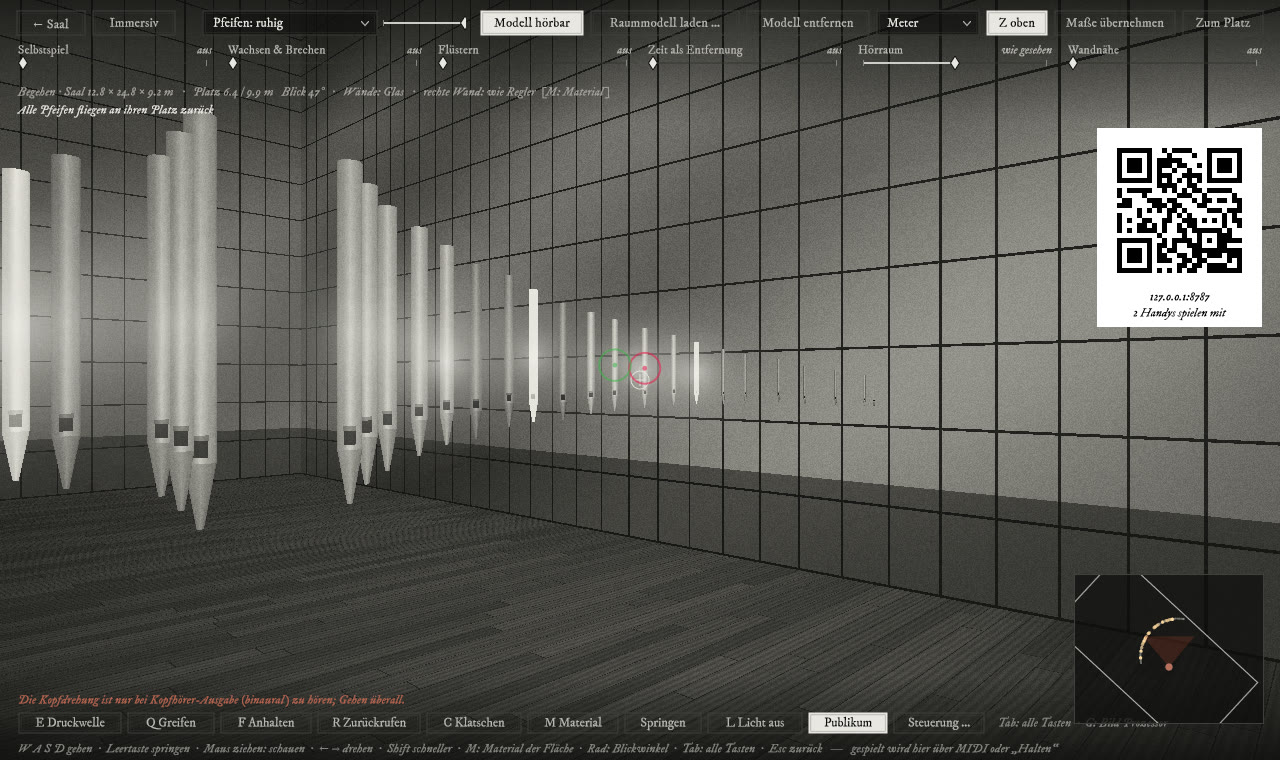
\includegraphics[width=0.8\linewidth]{screens/ui_begehen_publikum.jpg}
\caption{\ui{Publikum}: the QR code and the address in the corner (here the test tool's own address on the computer), two phones playing along, their
pipes marked with rings of their colours in front of the row.}
\label{fig:audience}
\end{figure}

% =====================================================================
\section{Effects}
\label{sec:effects}
% =====================================================================

The \ui{Effekte} page collects sounds that are easy to localise -- short, bright, rich in transients -- and
that follow the pipes, making their positions audible. Everything is off by default.

\begin{description}
  \item[Eigene Geräusche] the user's own recordings (up to 64 files of up to \SI{20}{s} in
        \fn{samples/noise/eigene}) are triggered by the keys. Each file is trimmed to its first
        transient and peak-normalised. They can sound at a pipe of a pulled stop, anywhere, at the
        console or circling; with a probability per key-down and key-up, pitch following the key,
        scattered delayed copies, and wandering around the listener.
  \item[Trakturweg] small ticks travel from the console to the pipes of the pulled stops, like the
        trackers of the mechanical action; with \ui{Pfeifen warten} a pipe only speaks when the path has
        arrived.
  \item[Knistern] short crackles at every sounding pipe, which move with the pipe; density per pipe
        and length per crackle. After release the crackle fades within half a second.
  \item[Windlecks] up to eight hissing leaks in the wind system at fixed (optionally wandering) places,
        swelling and fluttering unevenly. \ui{Gebläse ringsum} spreads the blower around the listener.
  \item[Obertöne verteilen] above a split frequency (a multiple of each pipe's fundamental) the
        sound of each pipe is moved sideways, randomly left or right per pipe, while the fundamental stays
        at the pipe; \ui{Kreisen} turns the upper part around the listener.
  \item[Wandernde Echos] up to eight repeats of the whole organ, each from the next direction
        (rotation and tilt per repeat), quieter and darker each time, with time free or synced to the
        tempo. Echoes also reach the room from their own direction.
\end{description}

\subsection{Effects of a single stop}
\label{sec:stopfx}
The tremulant, the crackle, the leaks and the speed of the motion used to be the same for the whole organ. The tab \ui{Pfeife} of the \ui{Raum} page,
which already held \ui{Ansprache}, \ui{Abriss} and the upper partials of \S\ref{sec:pipesound}, now gives every stop four more controls of its own,
which act on top of the global ones:
\begin{description}
  \item[Tremulant] a tremulant for this stop alone, at the tempo of the global tremulant (\ui{Klang} page); its depth is added per voice to that of the
        global one, which keeps running for the stops that have none of their own.
  \item[Knistern] crackle at the sounding pipes of this stop, added to the global density.
  \item[Windleck] two hissing leaks at the pipes of this stop, which sound while the stop is drawn and move with its pipes; they are rendered like
        the global leaks, at the place of the stop's pipes at that moment.
  \item[Tempo-Streuung] every pipe of the stop turns, tilts, swings or drifts at its own speed (\S\ref{sec:motion}).
\end{description}
\ui{für alle Register übernehmen} copies the four values to every stop. They are host parameters (\fn{pipeTrem}, \fn{pipeCrack}, \fn{pipeLeak},
\fn{pipeSpread} with the stop's number) and therefore modulation targets and lanes of the \ui{Verlauf}. The render test plays each of them alone,
and checks that a change of the speed spread moves no pipe.

\subsection{The output stage (\ui{Summe})}
\label{sec:summe}
The tab \ui{Summe} of the \ui{Effekte} page is a small mixing and mastering stage, the very last step of everything that goes out: stereo,
binaural, transaural, Ambisonics and loudspeakers alike (\fn{MasterBus.h}; Figure~\ref{fig:summe}).
\paragraph{Equaliser.} Three bands, each a biquad after the RBJ cookbook \citep{rbj}: a low shelf (\SIrange{30}{600}{Hz}), a bell
(\SIrange{150}{8000}{Hz}, \ui{Güte} $Q=0.2$--6) and a high shelf (\SIrange{1.5}{18}{kHz}), each $\pm\SI{15}{dB}$. The same filter runs on every
channel, so an Ambisonics field stays a field: a filter that is linear and equal on all channels commutes with the decoding. A flat band costs nothing.
The curve is drawn from the filters' own transfer functions.
\paragraph{Compressor.} A feed-forward compressor with threshold (\SIrange{-48}{0}{dB}), ratio (1--20), attack (\SIrange{0.1}{100}{ms}),
release (\SIrange{10}{1500}{ms}) and make-up gain (\SIrange{0}{24}{dB}). Its detector hears the loudest channel, sample by sample; the level in dB
follows it with the attack or release time constant, and the gain reduction for an overshoot $o$ above the threshold $T$ with ratio $R$ and a
soft knee of width $W=\SI{6}{dB}$ is
\begin{equation}
  g(o)=\begin{cases}0 & 2o\le-W\\[2pt] \bigl(\tfrac1R-1\bigr)\dfrac{(o+W/2)^2}{2W} & |2o|<W\\[6pt] \bigl(\tfrac1R-1\bigr)\,o & 2o\ge W,\end{cases}
\end{equation}
smoothed once more over \SI{2}{ms}. All channels are turned down by the same gain, so the spatial image does not move when the compressor works --
a compressor per channel would pull loud directions towards quiet ones. The page draws the static curve and how much is being turned down at the
moment. All controls are read through their modulated values, so LFOs and the lanes of the \ui{Verlauf} move them. In the check of the snapshot tool a
bell of \SI{+6}{dB} at \SI{1}{kHz} measures \SI{+6.00}{dB}, a low shelf of \SI{-6}{dB} measures \SI{-5.96}{dB} at \SI{30}{Hz} and leaves \SI{15}{kHz}
untouched (\SI{0.03}{dB}), and with a threshold of \SI{-20}{dB} and a ratio of 4:1 a sine at \SI{0}{dBFS} comes out at \SI{-14.9}{dB} (the formula gives
\SI{-15}{dB}; measured with an attack of \SI{0.1}{ms}).

\begin{figure}[!htb]
\centering
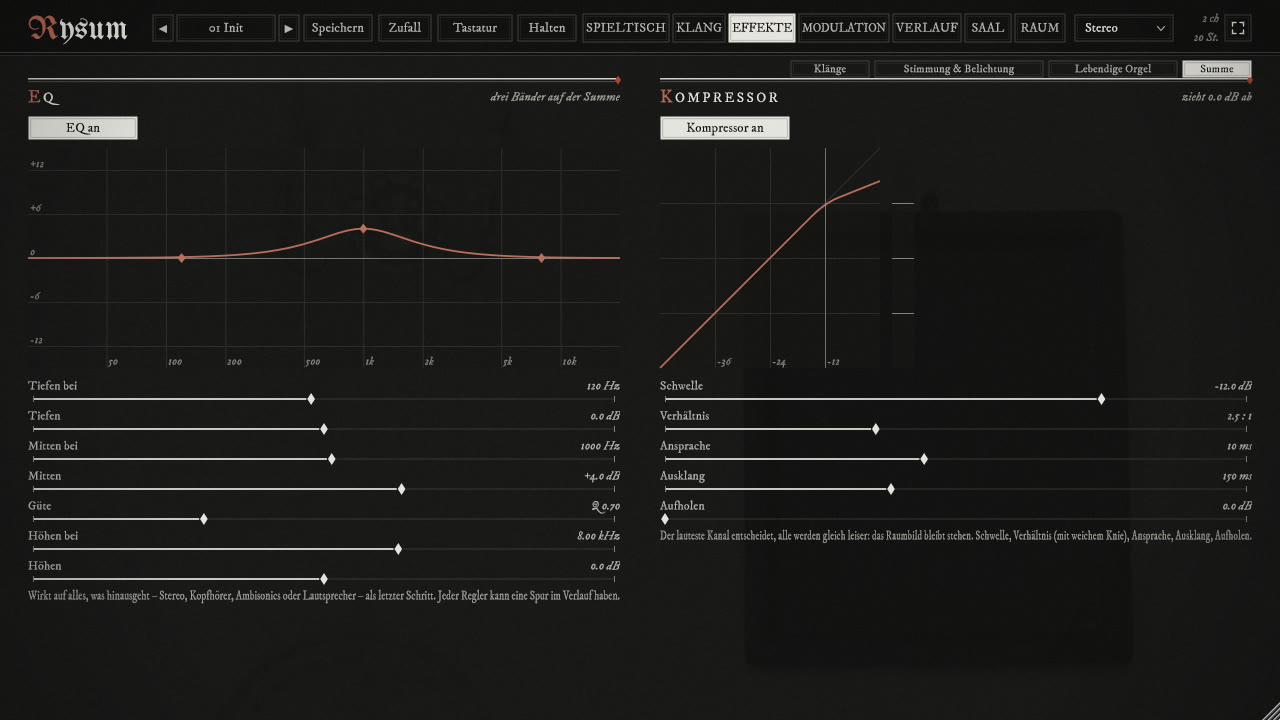
\includegraphics[width=\linewidth]{screens/ui_effekte_summe.jpg}
\caption{The tab \ui{Summe} of the \ui{Effekte} page: the equaliser with its curve, and the compressor with its static line and the meter of the gain
reduction.}
\label{fig:summe}
\end{figure}

\subsection{Tuning made audible and photographic operations (\ui{Stimmung \& Belichtung})}
\label{sec:exposure}
The second tab of the \ui{Effekte} page (everything off by default) contains effects that make the meantone tuning
audible in space, and two operations on the whole sound field borrowed from photography. They are described here from the
source code; the author's commit called them untested, and the render test of 15~November now checks each (\S\ref{sec:verification}).

\paragraph{Beats (\ui{Schwebungsraum}).}\label{sec:beats}
For every pair of sounding pipes with frequencies $f_1<f_2$ the engine looks for the lowest pair of partials that
nearly coincide: for $m=1\dots6$ it takes $n=\mathrm{round}(mf_2/f_1)\le8$ and keeps the pair with the smallest
$nm$ for which the beat $b=|nf_1-mf_2|$ is below \SI{35}{Hz}. Every pipe takes the fastest beat it has with any other
pipe; the rate is smoothed and offered in two ways: as the motion \ui{Schwebung} (\S\ref{sec:motion}), and as the
per-pipe modulation source \ui{Schwebung}, $\log_2(1+b)/\log_2 33$ (0 = still, 1 = \SI{32}{Hz}), so that the beats can
drive anything else -- for example \ui{Schwebung} $\rightarrow$ \ui{Pfeife: Verfall}, and impure intervals crumble.
\ui{Schwebungen aus} chooses between the tuning as it is meant (ideal frequencies) and the pipes as recorded, which are
only accurate to about $\pm5$ cents, so that even the pure thirds beat a little. Figure~\ref{fig:beats} shows the
rates this rule gives in ¼-comma meantone and, for comparison, in equal temperament.

\begin{figure}[t]
\centering
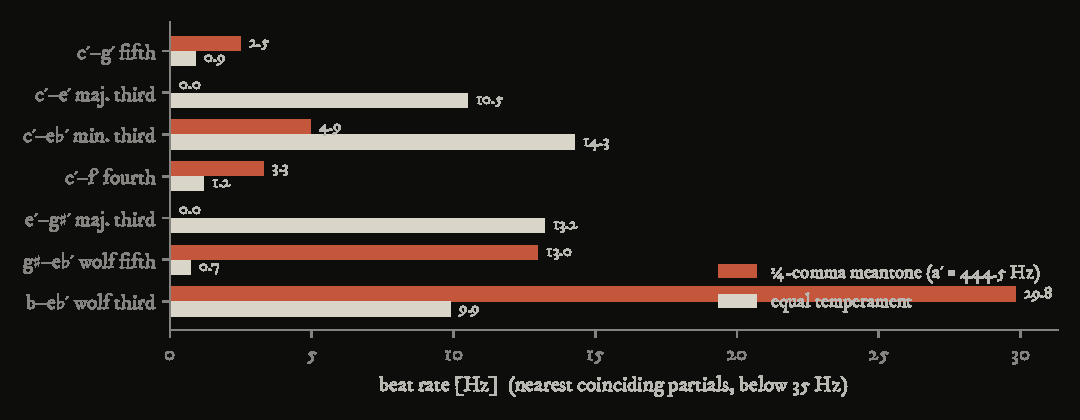
\includegraphics[width=0.92\linewidth]{figs/beats.pdf}
\caption{Beat rates of some intervals by the rule of \fn{updateBeats}, ideal frequencies, a′ = \SI{444.5}{Hz}. In
meantone the major thirds are pure and stand still, the fifths drift slowly, and the wolf intervals spin. A missing
bar means no coinciding partials below \SI{35}{Hz}.}
\label{fig:beats}
\end{figure}

\paragraph{Difference tones (\ui{Differenztöne}).} Every pair of \emph{held} pipes may sound its difference tone
$f_2-f_1$ (if it is at least \SI{16}{Hz} and not above $1.02f_1$), as the resultant with which organ builders suggest a
32′: a fifth gives the octave below its lower note, a pure third two octaves below the root of the triad. The pairs are
weighted by $\sqrt{g_1g_2}\,\bigl(1-\kappa+\kappa\,c\bigr)$ with the consonance $c=\min(1,6/(nm))$ of the pair found above
and $\kappa$ = \ui{nur Konsonanzen}; the twelve strongest sound, each a soft tone with a little second and third partial
(so that low ones are heard on small loudspeakers), fading in over about \SI{0.4}{s} and out over \SI{0.3}{s}. A ghost
keeps its pair and phase while the pair is held. \ui{Ort} places it between the two pipes (the direction of the sum of
their unit vectors) or, towards 1, deep below the listener. Below about \SI{80}{Hz} no Ambisonics system localises well,
so the deepest ghosts are felt more than located.

\paragraph{Tonnetz.} The layout of \S\ref{sec:layouts} belongs to this group in the interface.

\paragraph{Double exposure (\ui{Doppelbelichtung}).} The field of $T$ seconds ago (\ui{Abstand}, \SIrange{0.05}{8}{s},
read from a delay line per channel with linear interpolation; a changed time glides like tape) is turned about the
vertical axis by $\psi$ (\ui{Drehung}): each pair of channels $(l,m)$, $(l,-m)$ is rotated by $m\psi$. It may be mirrored
(\ui{Spiegeln}) by sign flips per channel: left/right flips the channels with $m<0$, front/back those with odd $|m|$
(sine and cosine parts with opposite signs), up/down those with odd $l+|m|$. A one-pole low-pass between \SI{18}{kHz} and
\SI{900}{Hz} fades the old image (\ui{Verblassen}), and it is added to the present with \ui{Menge}. With \ui{mehrfach
belichten} ($\le0.85$) the copy is written back into the delay line, so older and fainter images follow. Up to third order;
in stereo, mirroring swaps the sides.

\paragraph{Long exposure (\ui{Belichtung}).} The field is decoded to 24 directions (Fibonacci lattice, SN3D weights
$(2l+1)/24$). Every direction keeps what passes through it in its own comb filter (\SIrange{30}{71}{ms}, different for
every direction, so the trails have no common pitch) with damped feedback $g=10^{-3L/(T f_s)}$ for a \SI{-60}{dB} time $T$
(\ui{Belichtungszeit}, \SIrange{0.2}{60}{s}), a low-pass in the loop between \SI{700}{Hz} and \SI{16}{kHz}
(\ui{Helligkeit der Spuren}) and two diffusing all-passes; the 24 trails are encoded again and added. A pipe that moves
leaves a trail behind it, fast ones paint arcs and rings. Up to third order.

\subsection{The living organ (\ui{Lebendige Orgel})}
\label{sec:live}
Until here every pipe was an independent sample player. The third tab of the \ui{Effekte} page, \ui{Lebendige Orgel},
treats the organ as one physical thing (\fn{OrganLive.cpp}, \fn{LiveParams}): a wind supply shared by all stops, pallets that
open as the key is played, a listener who walks, pipes that wear out, silent pipes that ring along, a tuning that pulls
itself pure and a walker in the Tonnetz. Everything is off by default, so older projects sound as before. All of it
is made of host parameters, so it can be automated and modulated, and it is part of the patches except for the wear
and the listener's walk in the 3D view (see below). The values of the figures in this section come from a re-implementation
of the engine's update rules in Python (\fn{figs/make\_figs\_live.py}); they show what the code is meant to do, not a
measurement of the plug-in.

\paragraph{Balg (bellows).} \ui{Windverbrauch} of 0\,\% is the endless wind of before. Above that, every sounding pipe draws on
\emph{one} supply, low pipes and many stops the most. With the stop wind $w_s$, the pallet opening $o$ of the pipe (below) and
its pitch $f$, the demand is
\begin{equation}
  D = \sum_{\text{held pipes}} w_s\, o\ \mathrm{clamp}\!\left(\sqrt{261.6\,\mathrm{Hz}/f},\,0.35,\,3\right).
\end{equation}
The wind of every pipe is multiplied by the pressure $P\in[0,1]$, so that when it runs short all pipes become flatter,
quieter, duller and unsteady together (with the wind model \ui{instabil} (\S\ref{sec:windchaos}) also their edge tones).
The \ui{Windquelle} decides how the pressure arises:
\begin{description}
  \item[Gebläse] a blower feeds steadily. With the amount $b$ (\ui{Windverbrauch}) and the size $S$ (\ui{Größe des Balgs}, in seconds),
        \begin{equation}
          \tau = \max(0.03, 0.1\,S),\qquad
          \dot P = \frac{(1-P) - p\,P}{\tau},\qquad p = \frac{3\,b^2 D}{24},
        \end{equation}
        so that a chord pulls the pressure down for as long as it sounds, to the steady value $P = 1/(1+p)$, and lets it come
        back when the keys are let go. One pipe hardly moves it (Fig.~\ref{fig:bellows}, left).
  \item[Kalkant tritt] a bellows treader lifts the bellows every few seconds (\ui{Tritte} per minute, or \ui{im Tempo}: every 8, 4, 2 or 1
        bars, a half or a quarter). A tread fills the bellows in \SI{0.3}{s}; between treads the content $V$ sinks as
        the pipes use the wind, $\dot V = -b\,(D/12)/S$ (twelve pipes of medium pitch empty it in $S$ seconds at 100\,\%).
        The weight on the bellows keeps the pressure up until it is nearly down: the target of $P$ is
        $x^2(3-2x)$ with $x=\min(1,V/0.3)$, followed with a time constant of \SI{40}{ms}. Play too much and the organ runs out of
        breath until the next tread (Fig.~\ref{fig:bellows}, right). \ui{Trittgeräusch} is the thump of the tread at the console
        (a low-passed noise burst with a \SIrange{36}{82}{Hz} tone and a decay of about \SI{0.1}{s}).
\end{description}
The two bars on the page show the supply and the pressure; the modulation source \ui{Balg (Winddruck)} (0 = empty, 1 = full)
lets the pressure drive anything else.

\begin{figure}[ht]
\centering
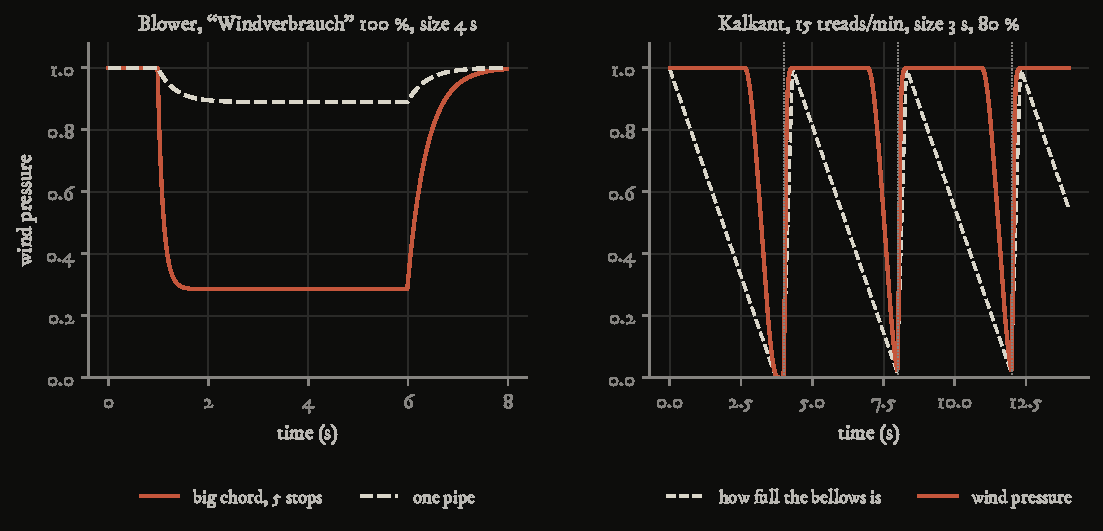
\includegraphics[width=\linewidth]{figs/bellows.pdf}
\caption{The wind pressure of the shared bellows, computed with the update rules of \fn{OrganLive.cpp}. Left: blower; a
big chord on five stops ($D=20$, the steady pressure is $0.29$) against one pipe ($D=1$, $0.89$) from 1~s to 6~s. Right: a
Kalkant treading every 4~s while a chord of twelve medium pipes is held; the dotted lines are the treads.}
\label{fig:bellows}
\end{figure}

\paragraph{Ventil (pallet).} The pallet under the pipe no longer opens instantly. With \ui{Anschlag} (source velocity) a slowly
pressed key lets the wind in hesitantly: with the pallet amount $a$ and $\mathit{slow} = (1-v)^2$ for the velocity $v$, the
pallet starts at $\max(0.1,\,1-a\,(0.3+0.7\,\mathit{slow}))$ and opens linearly within $T = 1.6\,\mathrm{s}\cdot a\cdot\mathit{slow}$.
The pipe speaks flat and dull (with the wind model \ui{instabil} of \S\ref{sec:windchaos} also breathy, with its mouth tone; in the
classic model \ui{Ventil} no longer switches those sounds on, as it did until 14 November) and only then finds its tone; a fast key speaks at once. With \ui{Druck} or \ui{Gleiten} the finger holds the pallet itself (MPE
pressure, aftertouch or CC~74): the opening follows the controller with \SI{12}{ms}, and the wind is $1-a\,(1-\text{opening})$;
at 100\,\% no pressure means no tone.

\paragraph{Hörer (listener).} The listener leaves the usual place. \ui{links / rechts} and \ui{zurück / vor} (metres, automatable and
modulatable) set where one stands; \ui{Hörer geht} walks around that place by itself (circle, left--right, forward--back, figure
eight; \ui{Tempo} in rounds per second, \ui{Weite} in metres). A new value is reached with a glide of \SI{120}{ms}, not by a jump. For a
pipe at azimuth $\varphi$, elevation $\vartheta$ and distance $d$, and a listener displaced by $(X,Y)$, the pipe is heard from
\begin{equation}
  x = -d\sin\varphi\cos\vartheta - X,\quad y = d\cos\varphi\cos\vartheta - Y,\quad z = d\sin\vartheta,
\end{equation}
that is from the direction and at the distance of this vector (never nearer than \SI{1}{m}, or than it was). Pipes one passes
become louder and brighter and move past, with Doppler; in the Saal the early reflections are heard from where one stands
(the room is re-evaluated with the displaced listener), while the late reverb stays that of the usual place. The little map
shows the pipes of the pulled stops and the listener (red). Clicks stay with the listener at the console, and the head still looks
forward: it is turned with \ui{Kopfdrehung}. Walls in non-convex plans hide pipes, see \emph{Out of sight} above.

\paragraph{Mitklingen (sympathetic pipes).} Silent pipes -- also those of stops that are not pulled -- ring quietly when a partial of a
sounding pipe meets their pitch. About twenty times a second the engine collects the first six partials of every held pipe
(weight $\min(2,g)/n$ for the $n$-th partial of a pipe with gain $g$) and compares them with the pitch of every silent pipe in the
current tuning: a partial within $25$\,ct adds $\mathit{weight}\cdot(1-\Delta/25\,\mathrm{ct})$. The sixteen best candidates ring,
each as a two-pole resonator at its own pitch (decay \ui{Nachklang}, the \SI{-60}{dB} time), excited by the sum of all
sounding pipes, and each from its own place. Pure intervals wake more pipes than impure ones, and another tuning wakes others.

\paragraph{Verschleiß (wear).} Every pipe remembers how long it has sounded: while it is held its wear $w\in[0,1]$ grows by
$\mathrm{d}t/(60\,M)$, with the \ui{Lebensdauer} $M$ in minutes; \ui{Wie stark man ihn hört} scales it to $w_r$. A worn pipe goes out
of tune, by up to $38\,\mathrm{ct}\cdot w_r^2$ (60\,\% of the pipes flat, the others sharp, each with its own factor), wavers
(the wind wobble of \ui{Verfall} gets $0.45\,w_r^2$) and crumbles with the grain, bit depth, sample rate and dropouts set under
\ui{Verfall} on the \ui{Spieltisch} (its amount grows by $w_r$), so the keys that a piece uses most fall apart first. The map shows
every pipe, one row per stop, worn ones in red. The wear is saved with the project, not with the patches (a patch does not make
the instrument young again); \ui{Alle Pfeifen neu} resets it. It only accumulates while the slider is above 0.

\paragraph{Reinheit (adaptive pure tuning).} Held notes pull each other towards pure intervals. For every pair of held notes (at
most 16) the nearest of eighteen pure intervals is looked up -- each with a weight $w$ (1 for the unison, fifth and octave, 0.9 for the
fourth, 0.8 for the major third, 0.6 for the minor third and the minor sixth, lower for the rest) and a reach (at most 20--45\,ct) --
and gives a spring of strength $w\,(1-|\mathit{dev}|/\mathit{reach})$ with the rest length of the pure interval. A weak spring of
strength $0.06$ holds every note at its tempered pitch, and the corrections $\delta_k$ are found by 24 sweeps
$\delta_k = \sum_j w_{kj}(\delta_j\pm e_{kj}) / (0.06+\sum_j w_{kj})$, with the mean removed so that the chord stays where it is.
New notes start in the chosen tuning and glide to their place with the time \ui{Zeit bis rein}; the beats calm down and the chord locks
in. Examples in quarter-comma meantone (computed with the same rule): in C--E--G the fifth, 696.6\,ct, is widened by 5.3\,ct to 701.9\,ct
while the pure third stays; in the chord G$\sharp$--B--E$\flat$, which contains the wolf fifth of 737.7\,ct, the fifth is brought back to
702.8\,ct (G$\sharp$ $+10$\,ct, E$\flat$ $-25$\,ct). With the motion \ui{Schwebung} the pipes stop turning as the chord becomes pure, and the
difference tones settle too (\S\ref{sec:beats}). The title of the tab shows the largest correction in cents.

\paragraph{Tonnetz-Wanderer.} While keys are held, a walker steps through the lattice of the tuning (fifths to the right, major thirds
up, \S\ref{sec:layouts}) and sounds every key it comes to, starting at the key struck last. At each step it moves to one of the six
neighbours (fifth up or down, major third up or down, minor third up or down); the \ui{Weg} chooses which: along the
fifths (after eleven steps: the wolf), a chain of thirds (major, minor, major, \dots), random, random with homesickness (of two
candidate steps it takes the one that leads back with probability 0.75), or a spiral around the first key (one fifth, one third, two fifths back,
two thirds back, three, \dots, then home again after 24 steps). The pitch class that the lattice point stands for is realised on the key nearest
to where the step leads, but never far from where the walk began. \ui{Schritt} is free (\ui{Tempo} in steps per second) or a note value of
the project tempo; \ui{Tonlänge} above one step lets the notes overlap (at most eight at a time). The player's own keys sound as usual.
With the arrangement \ui{Tonnetz} (\S\ref{sec:layouts}) the sound takes the same walk through the room. Since the tuning update every tuning
except the original one plays note by note (\emph{free mode}: the other tunings, Scala, MTS-ESP and MPE), and there the walker steps through MIDI
notes on the channel struck last, each sounding on its pipe as if it had been played (for a while after the tuning update it switched itself
off in these tunings; fixed on 15~November). The render test checks both ways.

\paragraph{Spieler bewegt die Pfeifen (the player and the pipes).} The listener -- the walked place of \ui{Hörer} or the camera of
the 3D view -- can act on the bodies of the room motions (\S\ref{sec:roommotion}): the controls \ui{Spieler bewegt die Pfeifen}
(here) or \ui{Pfeifen: \dots} (in the 3D view) choose the mode, \ui{Kraft} $F\in[0,1]$ (default 0.5) and \ui{Reichweite} $R\in[0.5,30]$\,m (default \SI{4}{m}).
A pipe at distance $d$ from the listener, with $\mathbf u$ the unit vector to the listener, is accelerated by
\begin{equation}
  a = \frac{30\,F\,R^2}{d^2 + 0.3\,R^2}\ \ \text{(m/s}^2)
\end{equation}
-- like gravity, but softened near the player: strong within the range, never endless. The four modes are
\begin{description}
  \item[zieht an] $\dot{\mathbf v} = a\,\mathbf u$: the pipes fall towards the listener.
  \item[stößt ab] $\dot{\mathbf v} = -a\,\mathbf u$: they flee.
  \item[Umlaufbahn] the pull of \emph{zieht an} (the vertical part halved), and in the horizontal plane the velocity is steered towards
        the listener's speed plus a circular speed $v_c=\sqrt{a\,d_h}$ around the upright axis ($d_h$ the horizontal distance), the speed
        that holds a body on a circle; the pipes circle the player.
  \item[Sog] a wake: near the player a pipe takes on the player's velocity, with the rate $6\,F R^2/(d^2+R^2)$ per second; a walking
        listener drags the pipes along.
\end{description}
Except in \emph{stößt ab} a pipe that comes within \SI{0.45}{m} is pushed back, never through the player. The force acts on the stops
whose motion takes place in the Saal (Flug, Fall, Schwarm, Strömung and Schweben); in the other modes the pipes still stay on the orbit
around the listening place. The listener's own speed is that of the walk, so a pipe is pushed along with a walking player. The player's
hands in the 3D view (\S\ref{sec:hands}) act on the same bodies, in single gestures rather than as a field.

\paragraph{Aufprall.} The knocking of pipes that fly through the room (\S\ref{sec:roommotion}) is also set on this tab.

Twelve factory patches (148--159) show all of this (Appendix~\ref{app:patches}). The whole group was written after the verification run
of 1~November; the render test of 15~November covers it (\S\ref{sec:verification}): with 24 pipes the blower's pressure falls to 0.26, the Kalkant's
bellows run empty before his first tread, a slow key is \SI{19}{dB} quieter than a fast one in its first \SI{0.4}{s}, wear after half a pipe's life is
0.5, sixteen sympathetic pipes ring \SI{6}{dB} below the struck one, pure tuning brings the fifth c′--g′ from \SI{2.46}{Hz} to \SI{0.06}{Hz} of beating
and the wolf from \SI{13.0}{Hz} to \SI{0.36}{Hz}, and the walker sounds fourteen keys along the fifths and leaves no voice behind.

% =====================================================================
\section{Live audio input}
\label{sec:input}
% =====================================================================

Live sound -- a voice, an instrument, another track -- can enter the plug-in and is placed and moved in the
same space as the pipes. The input is a source like a pipe: it has an azimuth, an elevation, a distance, a
spin in degrees per second around the listener and an optional room send; it receives distance gain, air
absorption and Doppler shift like a pipe (\S\ref{sec:spatial}). It then passes through everything that
follows the pipes: the simulated room or impulse response, the echoes, the \ui{Verfall} degradation of the
sum, the Lucier mode and the output format.

Input can be mono (one source) or stereo (two sources, a \ui{Breite} apart). Its place is either free or
bound to a stop (\ui{auf <Register>}): the input then rides on the pipes of that stop, the left channel on the
low side of the keyboard and the right on the high side, and it moves with their motion. With \ui{Tasten
öffnen} the input sounds only while keys are held, closing over a release time \ui{Ausklang}. The loudness of
the input after its level is a modulation source (\S\ref{sec:modulation}); it is measured on a scale from
\SI{-54}{dB} to \SI{0}{dB} with a \SI{10}{ms} attack and a \SI{200}{ms} release, and it is computed even when
the input itself is not heard, so a voice can open the organ's wind without being played through it.

In Reaper and Ableton Live the input is the audio the host routes to the instrument. The standalone
application takes it from an audio input device chosen in its audio settings, and its input mute must be
switched off; with loudspeakers the output would feed back, so headphones are advisable. In the effect version \emph{Rysum FX} the input is the track's audio and the input is on by
default. A patch made with the input switched on switches it on when loaded; other patches leave it as it is,
like the MPE setting. Patches 72--79 demonstrate the input. The input can also \emph{play} the organ: with \ui{Eingang spielt die Orgel} the
pitches that the neural pitch estimator of the \ui{Vox humana} hears in it become notes for the stops (\S\ref{sec:vox}).

% =====================================================================
\section{A neural stop (\ui{Vox humana})}
\label{sec:vox}
% =====================================================================

The dataset of \S\ref{sec:dataset} was rendered to train a neural network on the plug-in's own sound. The result is a ninth stop,
\ui{Vox humana 8$'$}, that has no samples: a network of 0.85 million parameters synthesises the organ from the keys that are held, and a second network
can listen to the audio input and find the notes in it. The model, its training and its evaluation are documented in a report of their own
\citep{neuralrysum2}, which is kept with the plug-in (\fn{docs/NeuralRysum\_v2\_paper.md}); this section summarises it and describes how the stop is
built into the instrument. The name is that of a historical reed stop that imitates the human voice.

\subsection{The model (NeuralRysum v2)}
A first version, an autoencoder with a fast learned code of 12 numbers every 64 samples and a slow timbre latent, did not resynthesise its input as an
organ: a singing voice came out as a noisier singing voice, because 9000 numbers per second are enough to carry a spectral envelope, and a model trained
only on organ audio has no reason not to copy it. Version~2 removes this path by construction (Figure~\ref{fig:vox}). The only link from the input
waveform to the output is a set of at most eight \emph{voices}, each a fractional MIDI key, a gate and the times since its onset and release:
\begin{description}
  \item[Pitch estimator] Four causal STFTs (windows of 512 to 4096 samples, hop 64) are resampled onto a log-frequency grid of three bins per semitone,
        each bin taken from the shortest window that still resolves a semitone there, and stacked at the positions of the harmonics $h\in\{\frac12,1,\dots,7\}$
        \citep{bittner2017salience}. A causal 2-D CNN of 17\,150 parameters gives a salience and an onset map over MIDI 21--108, 750 frames a second.
        It is trained only on synthetic sounds whose timbre is random in every example (harmonic tilt, odd harmonics, missing fundamentals, formants,
        inharmonicity, reverb, EQ and noise), so it carries pitch and nothing else.
  \item[Voice tracker] Plain code: peaks above a threshold, refined to fractional keys, are followed by the existing voices within 0.7 semitones (glides,
        vibrato, detuned pipes), held for \SI{32}{ms} through missing frames, and a new voice starts only after its peak has been seen in four consecutive
        frames (\SI{5.3}{ms}). Keys outside the organ's range are folded by octaves into C2--B5. MIDI produces exactly the same voices.
  \item[Organ synthesiser] Per voice and every 128 samples, an MLP (width 192, 189\,535 parameters) maps a learned embedding of the key, the onset and
        release times and the timbre to 511 harmonic amplitudes on \emph{half} the key's frequency and 32 noise-band gains, in the manner of DDSP
        \citep{engel2020ddsp}. One harmonic series on the 16$'$ pitch covers every rank of an organ (16$'$, 8$'$, 4$'$, 2$\frac23'$, \dots), so the one
        network can play a single flute and a full plenum with mixtures. The harmonics are played from a 1024-point wavetable made by an inverse FFT each
        frame and crossfaded over the hop, so the cost per sample does not grow with the number of harmonics; a learned impulse response of \SI{2}{s}
        is the organ's room.
  \item[Timbre] Eight latent numbers and three descriptors (brightness, noisiness, spread) describe the registration. In \emph{Manual} mode they are the
        stop's controls; in \emph{Follow} mode a slow encoder (one frame every \SI{42.7}{ms}) derives them from the input, so a brighter input makes a
        brighter organ, a channel of eleven numbers at 23\,Hz that cannot carry a waveform.
\end{description}
The synthesiser was trained for 150\,000 steps on the pipes and registrations of the dataset (multi-resolution STFT loss, from step 40\,000 also an
adversarial loss), with every note's real pitch measured from the audio, so that it plays the organ's meantone exactly when driven by MIDI. Sent
through non-organ signals (a sawtooth, sung vowels, a plucked string), the output has \SI{36.5}{dB} less energy above \SI{5}{kHz} than the input in
Manual mode (the first version: \SI{17.5}{dB}), 94\,\% of its energy below \SI{5}{kHz} lies on harmonics of the played note, and silence gives digital
silence. A note is detected after \SI{9}{ms} at C6 and \SI{33}{ms} at C2.

\begin{figure}[!htb]
\centering
\begin{tikzpicture}[
  box/.style={draw=ink2, line width=0.5pt, rounded corners=1.5pt, align=center, font=\footnotesize,
              minimum height=0.95cm, inner sep=3pt, text width=2.3cm},
  arr/.style={-{Stealth[length=1.8mm]}, line width=0.55pt, color=ink2},
  lab/.style={font=\scriptsize\itshape, text=muted}]
  \node[box, text width=1.5cm] (in) at (0,0) {Audio input};
  \node[box] (pe) at (2.9,0) {Pitch estimator\\ \scriptsize CNN, 17\,k par., hop 64};
  \node[box] (tr) at (6.1,0) {Voice tracker\\ \scriptsize $\le 8$ voices};
  \node[box, fill=rubric!30!bg] (sy) at (9.6,0) {Organ synth\\ \scriptsize 511 harmonics, 32 noise bands, room};
  \node[box, text width=1.6cm] (out) at (12.7,0) {Engine\\ \scriptsize placed like the input};
  \node[box, text width=1.5cm] (keys) at (6.1,1.6) {Keys\\ \scriptsize in the tuning};
  \node[box] (tim) at (9.6,-1.75) {Timbre\\ \scriptsize knobs (Manual) or encoder (Follow)};
  \node[box, text width=2.0cm] (stops) at (6.1,-1.75) {Sample stops\\ \scriptsize MIDI channel 16};
  \draw[arr] (in) -- (pe); \draw[arr] (pe) -- (tr); \draw[arr] (tr) -- node[lab, above]{key, gate, ages} (sy);
  \draw[arr] (keys.east) -| (sy.north); \draw[arr] (tim) -- (sy); \draw[arr] (sy) -- (out);
  \draw[arr] (tr) -- node[lab, right]{\ui{Eingang spielt die Orgel}} (stops);
  \draw[arr, dashed] (in.south) |- ($(tim.south west)+(0,0.2)$);
\end{tikzpicture}
\caption{The \ui{Vox humana}. Only key numbers, gates and two timers cross from the input to the synthesiser; the timbre comes from the stop's controls,
or, in Follow mode (dashed), from a slow encoder on the input. The voices the tracker finds can also play the sample stops.}
\label{fig:vox}
\end{figure}

\subsection{The stop in the plug-in}
The C++ engine (\fn{plugin/source/vox/}, header-only) is a port of the PyTorch reference: the estimator with an AVX2+FMA kernel for its convolutions,
the tracker, the synthesiser (the voice network batched over all voices, PFFFT for the wavetables, a fourth-order band-pass bank for the noise,
partitioned convolution for the room) and the Follow encoder; the weights are read from \fn{vox\_humana.nrv2}, which is embedded in the binary.
\fn{RysumVoxTest} compares it with reference vectors written by PyTorch: the estimator's logits agree within $1.4\times10^{-3}$, the tracker's decisions
are identical, MIDI rendering agrees within $3\times10^{-9}$ and tracked rendering within 1\,\% of the peak (phase drift from pitch differences of
$10^{-5}$ semitones). The glue (\fn{VoxStop.h}) runs the model at its own \SI{48}{kHz} around any host rate (four-point Hermite resampling in both
directions) and gives the held keys their fractional pitch in the plug-in's tuning -- every temperament, \ui{Stimmton}, Scala and MTS-ESP -- so the
neural stop is tuned like the pipes. Eight voices serve the keys and eight more the tracked input.

\paragraph{Controls.} On the \ui{Spieltisch} the stop has a knob like the others, with \ui{Lautstärke} and \ui{Wind}; less wind makes it duller, breathier
and quieter, like a half-drawn stop (the brightness descriptor falls by $0.6$ and the noisiness rises by $0.5$ at no wind). \ui{Vox \dots} opens its
timbre -- \ui{Klangfarbe X/Y} (the first two latent axes), \ui{Helligkeit}, \ui{Hauch} and \ui{Breite} (the three descriptors) and \ui{Klangfarbe folgt dem
Eingang} (Follow) -- and the options of the input: \ui{Eingang spielt die Orgel}, the detection threshold, the confirmation time and the number of voices.
On the \ui{Raum} page a row under the audio input places it: \ui{Lautstärke}, \ui{Hall-Anteil}, \ui{Richtung}, \ui{Höhe}, \ui{Abstand} and the share of its
own learned room, and its symbol in the top view can be dragged.

\paragraph{In the engine.} The \ui{Vox humana} is one more source like the audio input (\S\ref{sec:input}): it has a direction, a distance and a room send,
gets its own early reflections in the \ui{Saal} and passes through everything after the pipes. All its parameters form a target group of the modulation
matrix, and the engine reads their modulated values, so an LFO on \ui{Klangfarbe X} glides through the registrations; they can also have lanes in
the \ui{Verlauf}. With \ui{Eingang spielt die Orgel} the tracker's voices become MIDI notes on channel~16, folded into the organ's compass and skipping the
gaps of the short octave, which the pulled sample stops play: a voice sung into the plug-in is answered by the Praestant.

\paragraph{The 3D model.} The stop has no pipes, so the 3D view shows what the network does. Its eight voices are glass pipes in a row at its place, each
as long as an open 8$'$ pipe of the pitch it sings at that moment ($2.44\,\mathrm{m}\cdot2^{-(k-36)/12}$), so a tracked voice that glides visibly
grows or shrinks. Around each pipe sit eight collars, one per band of the harmonics on half the key's frequency (16$'$, 8$'$, 5$\frac13'$, 4$'$, 3$\frac15'$--2$\frac23'$,
2$\frac27'$--2$'$, 1$\frac79'$--1$'$ and higher, from the bottom up); a collar's width and brightness show that band's strength relative to the strongest,
so a flute lights mostly the 8$'$ collar and a plenum with mixtures the upper ones. A sounding pipe glows with its level and is a lamp when the
light is off. The synthesiser publishes key, level and the eight band energies per voice and frame for this, lock-free.

\paragraph{Measured in the plug-in.} \fn{RysumVoxRender} plays \SI{20}{s} of a full mix through the whole plug-in. The stop alone is about as loud
as one sample stop ($\SI{-28}{dBFS}$ RMS against $\SI{-25.7}{dBFS}$ for Gedackt and Octave together), without clicks. One core of the author's desktop
is loaded by 4\,\% with the \ui{Vox humana} played from the keys, 15\,\% with the input playing it, and 25\,\% with the input, Follow, the
\ui{Vox humana} and sample stops together. Its weaknesses are those of the model: the lowest octave is detected slowly and sometimes an octave too high,
repeated notes on the same key merge into one, a dense mix is reduced to its eight most salient pitches, and the stop knows one organ and one room
\citep{neuralrysum2}.

% =====================================================================
\section{Modulation and control}
\label{sec:modulation}
% =====================================================================

\subsection{Sources and targets}
The modulation system has four LFOs (sine, triangle, saw, square, random steps, smooth random; 0.01--20
Hz or synced to note values), two DADSR envelopes, and further sources: key position
($-1\dots1$), mod wheel, a random value per note, velocity per note, and pitch wheel ($-1\dots1$; it bends
nothing by itself and must be routed). With MPE (\S\ref{sec:mpe}) pressure and slide are sources per note, the loudness of the audio input (\S\ref{sec:input}) is one more, \ui{Schwebung} gives every pipe the rate at which it beats with the others (\S\ref{sec:beats}), and \ui{Balg (Winddruck)} is the pressure of the shared bellows (\S\ref{sec:live}). LFOs have a \ui{Versatz je Pfeife}: 0\,\% moves all pipes
together, 100\,\% spreads one full cycle across the pipes, along the keyboard (a wave running from bass
to treble) or randomly. Envelopes run either per pipe (every note its own) or globally (one envelope,
restarted by every key, released when all keys are up).

Twenty-four routings connect a source to a target with an amount of $\pm100\,\%$, either bipolar
(the source swings around the slider value) or unipolar (only pushes one way). Targets are
\begin{itemize}
  \item per-pipe targets that act on every pipe separately, at 100\,\% amount: direction ($\pm180°$), height
        ($\pm90°$), distance ($\times8$), level ($\pm\SI{36}{dB}$), pitch ($\pm12$ semitones), brightness
        ($\pm6$ octaves of the air low-pass), room send ($\pm\SI{24}{dB}$); the pipe's own stop wind, its amount of
        \ui{Verfall}, its \ui{Windschwankung} and its crackle ($\pm100\,\%$ each); and, in submenus, everything of the
        \ui{Pfeife} tab (\ui{Ansprache} $\pm1$, \ui{Schärfe}, \ui{Nur Ansprache}, \ui{Wiederholen}, \ui{Abriss} $\pm100\,\%$,
        \ui{Obertöne ab} $\pm4$ octaves, \ui{Pegel} $\pm\SI{24}{dB}$, \ui{Anschlag} $\pm100\,\%$, \ui{Luft umkehren}), of the grain
        cloud (\ui{Menge}, \ui{Dichte} and \ui{Korngröße} $\times8$, \ui{Streuung} $\pm180°$, \ui{Zeitstreuung} $\pm\SI{150}{ms}$),
        of \ui{Verfall} per pipe (\ui{Körnung}, \ui{Aussetzer}, \ui{Bittiefe} $\pm13$ bits, \ui{Abtastrate} $\pm6$ octaves) and
        of the glitches. These are added on top of the stop's setting. \ui{Wiederholen} and the hard start of \ui{harte Kanten} are
        read when the note starts, \ui{Abriss} and the hard release when the key is let go; everything else follows the
        modulation continuously;
  \item every continuous parameter of the plug-in (stop volume and wind, motion speed, \ui{Verfall},
        Doppler, room, effects, even the LFO rates), where the amount is a share of the slider's range.
\end{itemize}
Modulation is evaluated every 64 samples. A modulated slider shows each routing's range as a red bar
with a draggable lozenge at the full-amount end, and a white tick at the current value; right-clicking any
slider assigns a free routing directly. In the \ui{Raum} view the pipes are drawn where modulation puts
them.

\subsection{MIDI and computer keyboard}
\label{sec:control}
MIDI notes play the organ (\S\ref{sec:instrument}); velocity shapes the key clicks; the sustain pedal holds.
A fixed CC mapping can be enabled (Table~\ref{tab:cc}). In addition, any parameter can be MIDI-learned:
right-click $\rightarrow$ \ui{MIDI lernen}, or on the \ui{MIDI-Regler} tab with 32 assignments, each with
CC number and channel, a range (reversible), and a \ui{Taster} mode in which every press toggles between
the ends of the range (for pads and switches). A learned CC takes precedence over the fixed mapping.
Assignments belong to the setup, not the sound: they are saved with the project and in
\fn{Documents/Rysum/MIDI-Regler.xml} as the default for new instances, but not in patches.

\paragraph{MIDI buttons for any button.} Since 14~November every button of the interface, not only the parameters, can be put on a pad, a
controller button or a key. \textbf{Ctrl+M} (or a menu entry on the \ui{MIDI-Regler} tab) lays a veil over the interface in which every button is
framed (Figure~\ref{fig:miditasten}); one clicks a button and presses the MIDI button, and the button gets a red tag with what it listens to
(\enquote{CC 30 $\cdot$ K1}, \enquote{Note C2 $\cdot$ K10}). A right click removes an assignment, Ctrl+click operates the button as usual (to reach
another page), Esc ends; while assigning, MIDI buttons operate nothing. A MIDI button may send a controller (pressed means 64 or more) or a note; an
assigned note no longer plays a pipe, and such notes are copied out of the MIDI buffer on the audio thread without allocating. Switches that are
parameters (the stops, \ui{Saal an}, the effects' switches) become ordinary entries of the \ui{MIDI-Regler} list, flipped by each press, and work
while the window is closed. All other buttons -- pages, patches, \ui{Zufall}, full screen, the hands of the 3D view -- are clicked by the open
window; the buttons that act while held follow the MIDI button (down is held). A button is remembered by its place in the interface (the test
tool finds all 368 buttons with a path of their own), so an update that rearranges a page can make an assignment need repeating.

\begin{figure}[h]
\centering
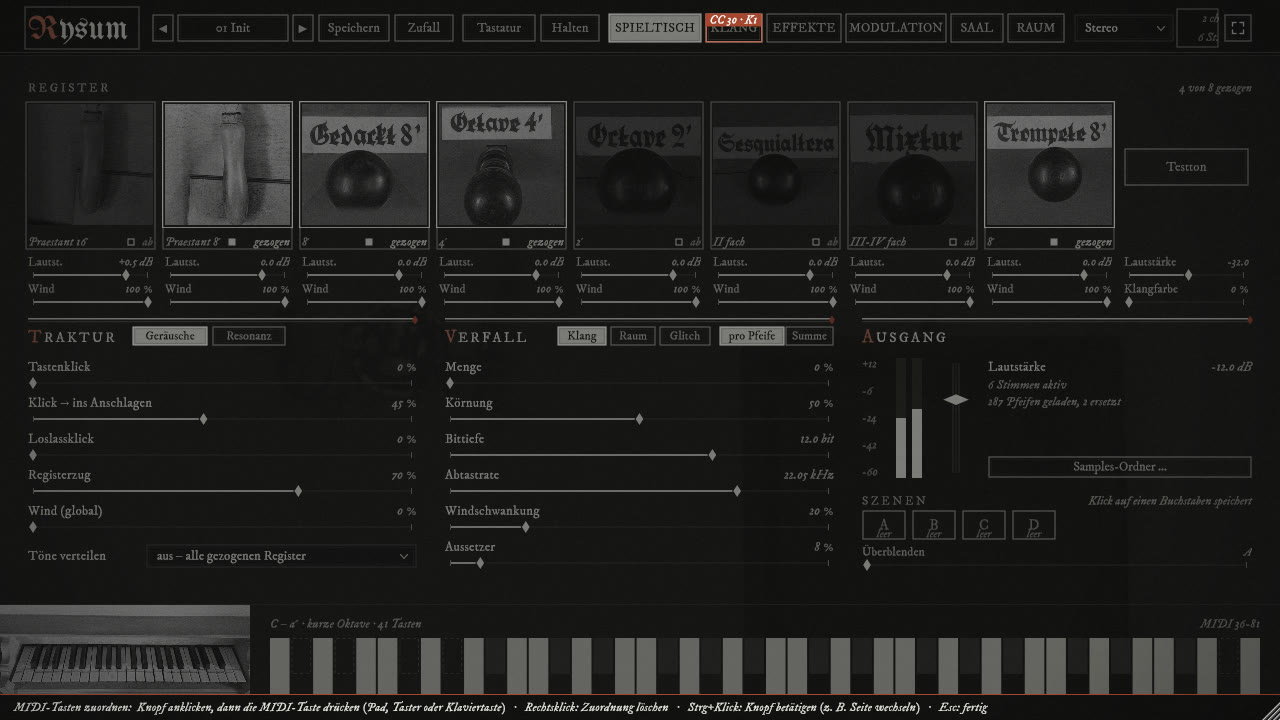
\includegraphics[width=0.85\linewidth]{screens/ui_midi_tasten.jpg}
\caption{Assigning MIDI buttons (Ctrl+M): a veil over the interface, every button framed; the page button \ui{Klang} carries the red tag of its
controller (\enquote{CC 30 $\cdot$ K1}), and the line at the bottom explains the clicks.}
\label{fig:miditasten}
\end{figure}

\begin{table}[h]
\centering\small
\begin{tabular}{@{}ll@{\hspace{2em}}ll@{}}
\toprule
CC & Function & CC & Function \\
\midrule
1     & tremulant depth (mod wheel)      & 27--33 & stop wind (same order) \\
11    & \ui{Wind (global)} / swell        & 34     & Praestant 16′ wind \\
19    & Praestant 16′ on/off              & 64     & sustain \\
20--26& stops on/off (Praestant \dots\ Trompete) & 66 & \ui{Freeze} (sostenuto) \\
\bottomrule
\end{tabular}
\caption{Fixed MIDI CC mapping (\ui{MIDI-CC an}).}
\label{tab:cc}
\end{table}

Two functions in the top bar help when no MIDI keyboard is at hand or both hands are needed elsewhere.
\ui{Tastatur} turns the computer keyboard into a manual (German layout: \code{A W S E D F T G Z H U J K O
L P} from C to d♯, \code{Y}/\code{X} octave, \code{C}/\code{V} touch). \ui{Halten} holds a note when its key
is struck twice quickly, exactly as if the key stayed down -- unlike \ui{Freeze}, the pipes keep sounding
normally, so stops, wind and modulation can be changed with free hands. Striking the key again releases it.

\subsection{Distributing notes (\ui{Töne verteilen})}
\label{sec:spread}
Normally every pulled stop sounds each note. With \ui{Töne verteilen} (console, \ui{Traktur}) every note goes to
a \emph{single pipe of one stop}, so that a chord is spread over the stops, and, with the four rooms of
\S\ref{sec:plans}, over different rooms. Three modes choose the stop: \ui{der Reihe nach} (the first note on the first
pulled stop in console order, the second on the next and so on), \ui{nach Lage} (by the position in the chord at the
moment it is played: the lowest held note on the first stop, the next above on the second, \dots) and
\ui{zufällig} (a random stop, never the same twice in a row). Muted pipes are skipped, so the note goes to the next stop
that has that pipe, and pulling a stop while notes are held does not add them to it.

\subsection{MPE}
\label{sec:mpe}
MPE (MIDI Polyphonic Expression, used by controllers such as the Lumatone, LinnStrument, Seaboard and
Osmose) gives every note its own MIDI channel. With \ui{MPE} switched on (\ui{Klang} page), each note on
channels 2--16 is bent, pressed and slid on its own. A pitch bend moves only its note: the bend
$b\in[-1,1]$ of the note's channel is multiplied by the bend range \ui{MPE-Beugung} (default 48 semitones, as
most controllers send, up to 96) and smoothed per slice. The pipe that plays the note is shifted, not replaced,
so a long slide sounds like a pipe being pitched rather than like a sequence of pipes. Channel pressure,
polyphonic aftertouch and MPE pressure are sources per note, and the slide (CC~74) is a second one; both can
be routed on the Modulation page. Channel~1 remains the instrument as a whole: its pitch wheel is the
\ui{Tonhöhenrad} source, and its tuning applies to all channels. With a free tuning the note channels use the
note numbers of channel~1's tuning. The MPE setting and its bend range belong to the controller and are not
stored in patches. Patches 64--67 demonstrate pressure and slide. The pitch bend failed the offline test of 1~November; in the run of
15~November a bend of $+2$ semitones on channel~2 gives \SI{196.9}{ct} while a note on channel~3 stays put, and with MPE off a bend leaves the note
unchanged (\S\ref{sec:verification}). MPE has still not been tried with a hardware controller.

\subsection{Scenes and random settings}
\label{sec:scenes}
\emph{Scenes} are four snapshots, \ui{A} to \ui{D}, of the whole sound. Every parameter is stored except the
output format, master volume, tuning, MIDI and headphone setup, the input switch and the MPE setting, so the
player's own setup is never changed by a scene. Clicking an empty letter on the \ui{Spieltisch} stores the
current sound there; clicking a stored one recalls it. The control \ui{Überblenden} moves continuously
between the stored scenes: with the position $x$ between two neighbouring stored scenes $A$ and $B$ and
$t=(x-A)/(B-A)$, continuous parameters are interpolated linearly, $v=(1-t)\,v_A+t\,v_B$, while switches and
choices change at the midpoint. Empty slots are skipped. The control is an ordinary host parameter, so it can
be automated, MIDI-learned or driven by an LFO. Only moving the control blends; between two moves the sound
can be edited freely and stored again. Scenes are saved with the project and in patches. Patches 68--71
demonstrate them.

The \ui{Zufall} button in the top bar sets random values, in two strengths. \ui{Sanft} takes small steps away
from the current sound: each continuous parameter moves by a Gaussian step of about 7\,\% of its range, and each
switch changes with a probability of 12\,\%. \ui{Wild} sets everything anew but keeps the result playable:
each stop is pulled with a probability of 45\,\%, at least one stop is always pulled, stop volumes lie between
$-12$ and $+6$\,dB, stop wind between 30 and 100\,\%, motion modes are drawn only where a path exists, and the
effects are mostly off or moderate. The dice work only on the groups that are ticked in the menu (Register,
Raum, Saal, Klang, Traktur und Verfall, Effekte, Modulation, Lucier and Eingang); master volume, output, tuning,
\ui{Freeze}, MIDI, scenes and pipe layouts are never touched, and routings without a source or target are left
alone. \ui{Zurück zum Klang davor} undoes the last roll.

% =====================================================================
\section{Automation over time (\ui{Verlauf})}
\label{sec:verlauf}
% =====================================================================

Modulation (\S\ref{sec:modulation}) moves controls periodically or in answer to the keys; what it cannot do is change many controls exactly,
slowly and together over minutes. The \ui{Verlauf} page does this, in the manner of the automation lanes of a host, but inside the plug-in and with
things a hand cannot do: loops of different lengths against each other, gestures that run through the room, variation from pass to pass
(Figure~\ref{fig:verlauf}). It is meant for performing first -- for textures that keep moving while one plays -- and not yet for writing whole pieces.

\begin{figure}[!htb]
\centering
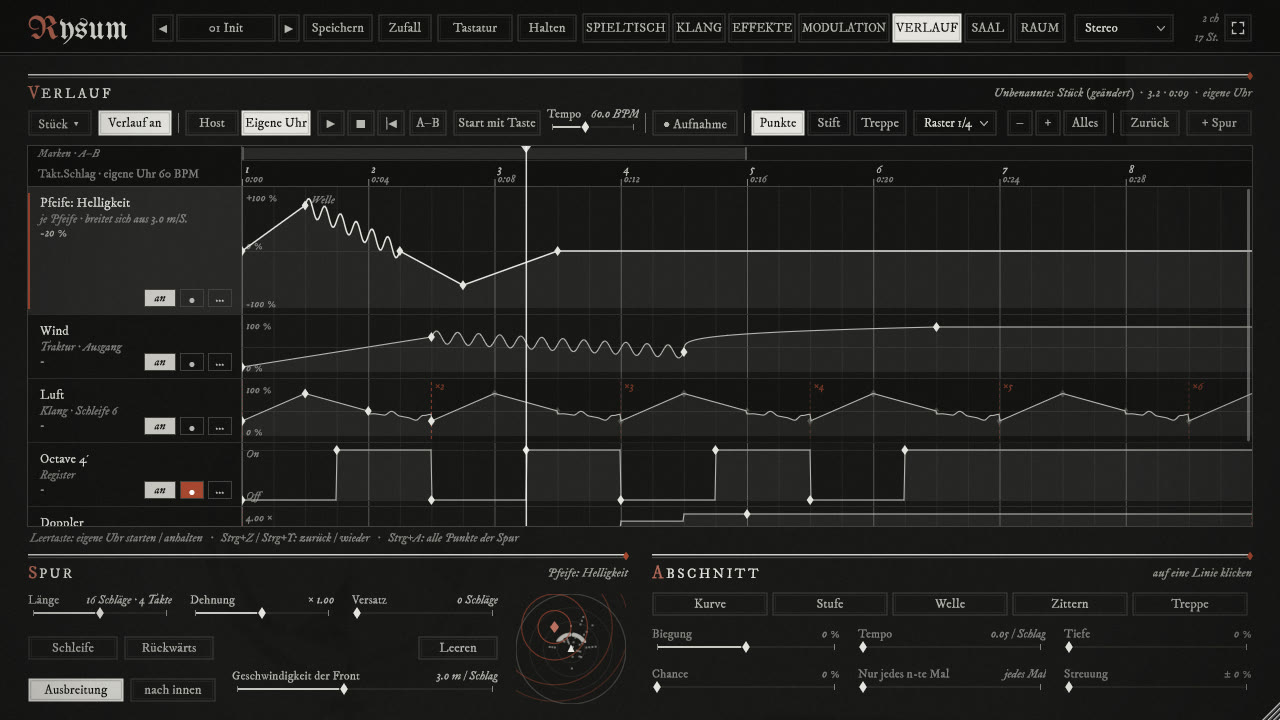
\includegraphics[width=\linewidth]{screens/ui_verlauf.jpg}
\caption{The page \ui{Verlauf}. Top: the menu \ui{Stück} and the bar with clock, recording, tools, grid and view. Below it the band of markers and
the ruler in bars and beats with the seconds of the own clock, then the lanes, each with its head (\ui{an/aus}, the record button, the lane's menu) and the
meaning of its top and bottom: a gesture of brightness that spreads through the room, with a \ui{Welle} section; the wind; a looping lane whose repeats
are marked; a stop switched on and off. The line under the lanes says what the mouse can do. Bottom: the lane (\ui{Spur}) with the plan of the spreading
front, and the chosen section (\ui{Abschnitt}) with its shape and its variation from pass to pass.}
\label{fig:verlauf}
\end{figure}

\subsection{Lanes, points and shapes}
A lane belongs to one control (up to 16 lanes): any slider, and of the switches those that act within a block -- the stops, the motion of each stop and its
\ui{harte Sprünge}, \ui{Freeze}, the tremulant and the wind model. The controls of the \ui{Saal}, the Lucier mode, the tuning and the IR switches have
no lanes, because they are read once per block or rebuilt in the background. A lane \emph{takes its control over} while it is on: the slider follows the
curve, modulation is added on top as it is on the slider, and grabbing the slider makes the lane give way for as long as one holds it. A lane is a list
of points (time in beats, value $0\dots1$); the section from one point to the next has one of five shapes:
\begin{description}
  \item[Kurve] a straight or bent line, $v=v_0+(v_1-v_0)\,u^{\,2^{-3b}}$ with $u$ the position in the section and the bend $b\in[-1,1]$ (from $u^8$
        to $u^{1/8}$);
  \item[Stufe] holds, then jumps;
  \item[Welle] the line plus a sine of a given number of waves per beat and depth;
  \item[Zittern] the line plus a smooth random wandering, the same every time the section is played, so that a bounce sounds like the playback;
  \item[Treppe] the line in steps.
\end{description}
A lane has a length, can loop, run backwards, be stretched (\ui{Dehnung}) and offset; lanes of different lengths and stretches drift against each other.
On the message thread the lanes are compiled into an immutable table, which the audio thread picks up at the start of a block and evaluates once per
slice of 64 samples; switches are rounded to steps.

\subsection{Clocks}
\ui{Host} follows the host's song position in beats, also when it stands still (the value at the cursor). The plug-in's own clock (\ui{Eigene Uhr}),
which the standalone uses, has play, stop and return, \ui{Start mit Taste} (the first key starts it) and its own tempo. Its tempo can itself be a lane,
\ui{Tempo der eigenen Uhr} (20--300 BPM), which the clock integrates: accelerandi, ritardandi, a sudden half time; the ruler's seconds follow it.
The ruler counts bars and beats with either clock.
A band above the ruler holds named markers (set with a double-click or \textbf{M}, jumped to with a click or \textbf{Bild auf/ab}), and dragging in it
lays a repeated section A--B: while \ui{A--B} is on, the own clock runs from A to B and round again.

\subsection{Writing the curves}
Points are set with a click on the grid and dragged; a click on the line chooses its section and dragging the line bends it; \ui{Stift} draws freehand
(the line is thinned to the points that matter) and \ui{Treppe} one step per grid cell. Several points are chosen with a frame, moved together,
copied and pasted. The lane's menu transforms a selection (stretch, squeeze, reverse, mirror, towards the middle, apart, onto the grid, a little off at
random), fills the loop with a pattern (a wave, a random walk, random steps, ramps, Euclidean rhythms such as 3 of 8 or 5 of 16), copies the curve to
another control, and sets a lane \emph{solo}. With \ui{Aufnahme} on, an armed lane records the hand: the movement of its slider is written while the
clock runs (only where it was moved, also into a lane that runs backwards) and thinned to a few points; a control without a lane gets one, armed, the
moment it is touched. A line of hints under the lanes always says what the mouse can do where it is, and a small readout shows the time and value under
the mouse. Undo and redo keep zoom and grid as they are.

\subsection{Variation from pass to pass}
In a looping lane each section can vary between the passes of the loop: \ui{Chance} -- in that share of the passes the section moves, in the others it
holds its start value; \ui{Nur jedes $n$-te Mal}; \ui{Streuung} -- the point's value wanders by up to that much from pass to pass. Each decision is a
hash of the lane's seed, the point and the number of the pass, so every pass decides anew but the same way every time it comes round: seeking and
bouncing give the same result. \ui{Variationen neu würfeln} gives the lane a new seed.

\subsection{Gestures in space and timetables}
A lane on one of the per-pipe targets of the modulation matrix (direction, height, distance, level, pitch, brightness, wind, \ui{Verfall} \dots) can
\emph{spread through the room}: the middle of the lane means no change, top and bottom the target's full swing, and with \ui{Ausbreitung} the gesture
starts at an origin and runs outwards as a front. Pipe $k$ at distance $d_k$ from the origin hears the curve at $t-d_k/c$, with the front's speed
$c$ in metres per beat; \ui{nach innen} lets the front come from \SI{25}{m} towards the origin. One swell of brightness then ripples through the case,
nearest pipes first, and a slow front turns one gesture into a canon in space. Moving pipes hear the front where they are at that moment. A small plan
on the page places the origin and shows the fronts passing. A stop that follows a drawn path (\S\ref{sec:motion}) can get a \ui{Fahrplan}: a lane
\ui{Bahn} whose value is where on its path the stop is at each moment, instead of running at a fixed speed. Its points appear as marks with their times
on the path in the \ui{Raum} view and can be dragged along it; two marks at the same place make the stop wait there, and every shape works on the
journey (\ui{Stufe} jumps, \ui{Welle} shivers back and forth along the path, a loop is a round trip).

\subsection{Pieces}
The lanes are saved with the project, not in patches. A \emph{piece} -- the lanes, the clock and its tempo, the markers and the drawn paths that its
timetables ride on -- can be kept as a file of its own (\fn{Documents/Rysum/Stücke/<name>.rysumstueck}) through the menu \ui{Stück}: new, open, save
(\textbf{Ctrl+S}), save as. The title shows the piece's name and \ui{(geändert)} while it has unsaved changes, and switching to another asks first. Six
pieces come with the plug-in, all started by the first key: \ui{Atem} (three stops breathe at 12, 16 and 20 beats, and their light with them),
\ui{Welle durch den Raum} (a swell of brightness runs from the front through the room every 8 beats, and a wave of loudness comes back from far away),
\ui{Registerkanon} (five stops come and go in loops of 12 to 36 beats), \ui{Verfall} (over 64 beats the organ crumbles, detunes and gets unsteady
wind), \ui{Schwebung} (the tremulant comes in, swells and drifts, and the pipes beat) and \ui{Fahrt} (the Praestant rides an arc in front of the listener
on a timetable, louder and brighter as it comes near).

\paragraph{Checks.} The snapshot tool drives the page with mouse events: clicks, the line, the frame, moving, deleting and undoing, pasting, heights,
hints, a lane created by recording, a marker and A--B set by mouse, and a Euclidean fill (5 of 8 gives 5 hits). On the processor side it checks the own
clock (one second is 1.003 beats at 60 BPM), the host clock (stopped and playing), loops, stretch, reverse and jitter, a hand
that makes a lane give way and is recorded, an LFO on top of a curve ($0.3\dots0.7$ around the curve's 0.5), a stop pulled by a lane, the tempo lane
(one second at 120 BPM is 2.005 beats), A--B, solo, chance (50\,\% moves in 100 of 200 passes), every third pass and \ui{Streuung}, the spreading
fronts (near pipes reached before far ones, inwards the other way round), a timetable, saving and reloading the project, a slider following its curve in
a real window, and that all six pieces load and drive real controls, \ui{Fahrt} brings its path, a saved piece loads back the same and a new one is empty.

% =====================================================================
\section{Playing for listeners on other computers (\ui{Konzert})}
\label{sec:konzert}
% =====================================================================

The audience of \S\ref{sec:audience} takes part from phones in the same room. \ui{Konzert} is for listeners on other computers, each in the 3D Saal
of their own: one person plays, the others listen, and \emph{no sound travels over the network, only the playing}. Every listener's computer renders the
organ itself, from wherever that listener stands and walks, with their own output -- headphones, loudspeakers, AmbiX.

\begin{figure}[!htb]
\centering
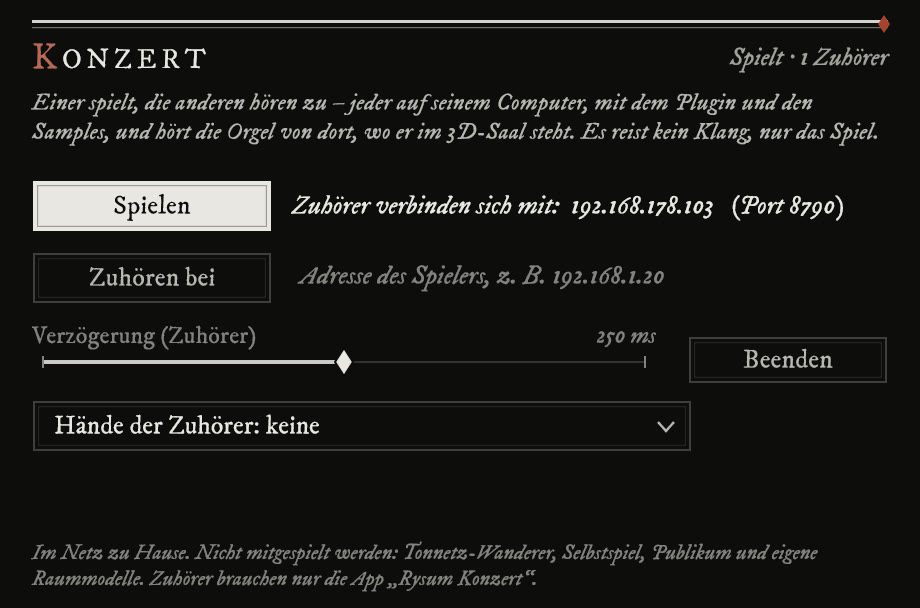
\includegraphics[width=0.72\linewidth]{screens/ui_konzert.jpg}
\caption{The window \ui{Konzert}, here playing for one listener: \ui{Spielen} with the address listeners use, \ui{Zuhören bei} with the player's address,
the listener's delay, \ui{Beenden}, and what listeners may do with their hands.}
\label{fig:konzert}
\end{figure}

\paragraph{What is sent.} The player's standalone (\ui{Konzert \dots} in the patch menu, \ui{Spielen}) accepts listeners on TCP port 8790 and sends
them, in framed messages, what makes the piece: the whole state when a listener joins and whenever something changes that is not a parameter (a
patch, a layout, a drawn path, a \ui{Verlauf} edit); every parameter change; the MIDI it plays, after \ui{Halten} and the controller assignments, so the
computer keyboard and the on-screen keys count too; and twenty times a second the clocks that move things -- the motion phases of the stops, the LFOs and
the \ui{Verlauf} clock --, so that pipes fly in the same places at the same moments. Everything carries the player's audio time. A listener plays
it a fixed delay later (\ui{Verzögerung}, \SI{250}{ms} by default, \SIrange{60}{2000}{ms}) through a jitter buffer, in the order it was sent, with
state changes as barriers: what comes after a state change waits until it has been applied on the message thread. The estimate of the offset between
the two clocks rises at once and comes down gliding, so a message that happens to arrive early does not shift the rhythm. Notes that are held when
someone joins sound for them too. Settings that belong to the listener stay theirs: output format, headphone and loudspeaker settings, volume, the
samples folder and where they stand; their own setup comes back when they leave, and saving while listening keeps it rather than the player's piece.
A broken or stalled link releases the notes and rejoins, and nothing left over from an old connection is played.

\paragraph{Hands, figures and the input.} Pipes that are bodies in the Saal (\S\ref{sec:roommotion}) follow the player's places, sent 50 times a second
while they move, instead of the listener's own physics; knocks, claps, bowed pipes and the lengths of \ui{Wachsen \& Brechen} come along and are heard from
the listener's place. Everyone in the Saal is a figure the others see, turned the way they look and with their name (red dots on the map): listeners send
where they stand and look ten times a second and the player passes this on to all. The player chooses what listeners may do with their hands --
nothing (the default), knock, push and clap, or also carry, throw, call home, whirl and sound pipes. A listener's act goes to the player, whose physics
stays in charge, and its result reaches everyone; a pipe in the listener's own hand follows that hand at once on their own screen. While the player's audio
input is on, it travels as 16-bit audio on the player's clock (about \SI{1.5}{Mbit/s} per listener), and every listener places and processes it
themselves, in time with the notes; a small adaptive resampler absorbs other sample rates and clock drift, and the Lucier mode may run at the listener on
that input. The Tonnetz walker and \ui{Selbstspiel} stay off at listeners, since they would play notes of their own; MIDI Tuning SysEx, the phone
audience and imported room models other than the six built-in ones are not mirrored.

\paragraph{The listener's program.} Listeners need neither the organ's controls nor MIDI: \emph{Rysum Konzert} (\fn{ListenerApp.cpp}) is a program of its
own that is only the 3D Saal and a line to join a player -- address, \ui{Zuhören}/\ui{Verlassen}, delay, output, volume and the audio device --, shipped as a
zip with the samples next to it (CMake target \fn{RysumKonzertZip}). A listener walks, looks, jumps and switches the light; the room and the Saal's
settings are the player's. The test (\code{RYSUM\_ONLY\_CONCERT}, \S\ref{sec:verification}) connects a player and a listener on the computer's own
address and drives the listener from its own audio thread. For now this is for one local network: a player on the internet would need a relay server,
and both sides must run the same version.

% =====================================================================
\section{User interface}
\label{sec:ui}
% =====================================================================

The interface is designed in black and white with grainy photographs of the organ, in the spirit of the
author's visual references in black-and-white photography and digital decay. The text face is
\emph{IM Fell DW Pica} (extended with arrows, primes and accidentals and renamed \enquote{Rysum Fell} as the
SIL Open Font License requires), the title is set in \emph{UnifrakturMaguntia}. Section headings have red
initials and double rules, slider handles are lozenges, the whole interface has a slight vignette. All
pop-up menus and dialogs use the same look. The window can be enlarged up to twice its size or shown full
screen (\code{F11}). Every value can be typed in its displayed unit (\enquote{300 ms}, \enquote{1.5 s},
\enquote{440} on \ui{Stimmton} for $a'$ in Hz), a double-click resets to the default.

The top bar holds the patch browser, \ui{Tastatur}, \ui{Halten}, the dice \ui{Zufall}, the page tabs (since 15 November seven: the six of before and
\ui{Verlauf}, \S\ref{sec:verlauf}), the output format and the full-screen button. The patch menu also opens \ui{Konzert \dots} (\S\ref{sec:konzert}) and
\ui{Alles zurücksetzen \dots}; the \ui{Effekte} page has a further tab \ui{Summe} (\S\ref{sec:summe}), the tab \ui{Pfeife} of the \ui{Raum} page also holds
the effects of a single stop (\S\ref{sec:stopfx}), and the \ui{Vox humana} sits on the \ui{Spieltisch} beside the stops and has a row of its own on the
\ui{Raum} page (\S\ref{sec:vox}). Clicking the name \ui{Rysum} in the top left opens a page about the organ itself: its history, its stops, where their pipes come from, and photographs. Scenes sit on the \ui{Spieltisch} page under \ui{Ausgang}, the Lucier controls in the middle column of \ui{Saal}, and the audio input in the last row of \ui{Raum}. A further page, \ui{Lautsprecher}, for the loudspeaker layout (\S\ref{sec:allrad}), opens from the channel display next to the output menu,
and another, \ui{Begehen}, the Saal in 3D (\S\ref{sec:walk}), from the floor plan of the \ui{Saal}. The \ui{Klang} page has a box \ui{Zwei Lautsprecher}
for the transaural output (\S\ref{sec:transaural}), a box \ui{Testton} for the reference tone (\S\ref{sec:testton}; its switch is also on the \ui{Spieltisch}), a switch \ui{Erweiterter Bereich} (\S\ref{sec:tuning}), the \ui{Effekte} page a third tab \ui{Lebendige Orgel} (\S\ref{sec:live}), and the \ui{Raum} page a
row \ui{im Saal} with the four room motions (\S\ref{sec:roommotion}). The page \ui{Begehen} has grown into an instrument of its own, with its
row of hands, the illusions, \ui{Immersiv}, \ui{Publikum} and \ui{Steuerung \dots} (\S\ref{sec:walk}, Figures~\ref{fig:walk}--\ref{fig:audience}); \textbf{Ctrl+M}
assigns any button to MIDI (\S\ref{sec:control}). The interface is redrawn 60 times a second.
\textbf{Ctrl+Shift+P} shows a readout of the drawing (pictures per second, milliseconds per picture, how much of the window is redrawn, whether the
interface thread falls behind, the renderer -- Direct2D or software -- and the pixel scale) and appends it once a second to
\fn{Documents/Rysum/paint-stats.txt}; \textbf{Ctrl+Shift+R} switches the renderer for comparison. The pages no longer repaint every row every frame, only
when something in them changed. Figures~\ref{fig:ui1}--\ref{fig:ui3} show the six main pages of version 12 (the \ui{Verlauf} is in Figure~\ref{fig:verlauf}); Figures~\ref{fig:uisaal}--\ref{fig:uiorgel} show the \ui{Saal} page with the Lucier controls, the audio input and the organ page.

\begin{figure}[p]
\centering
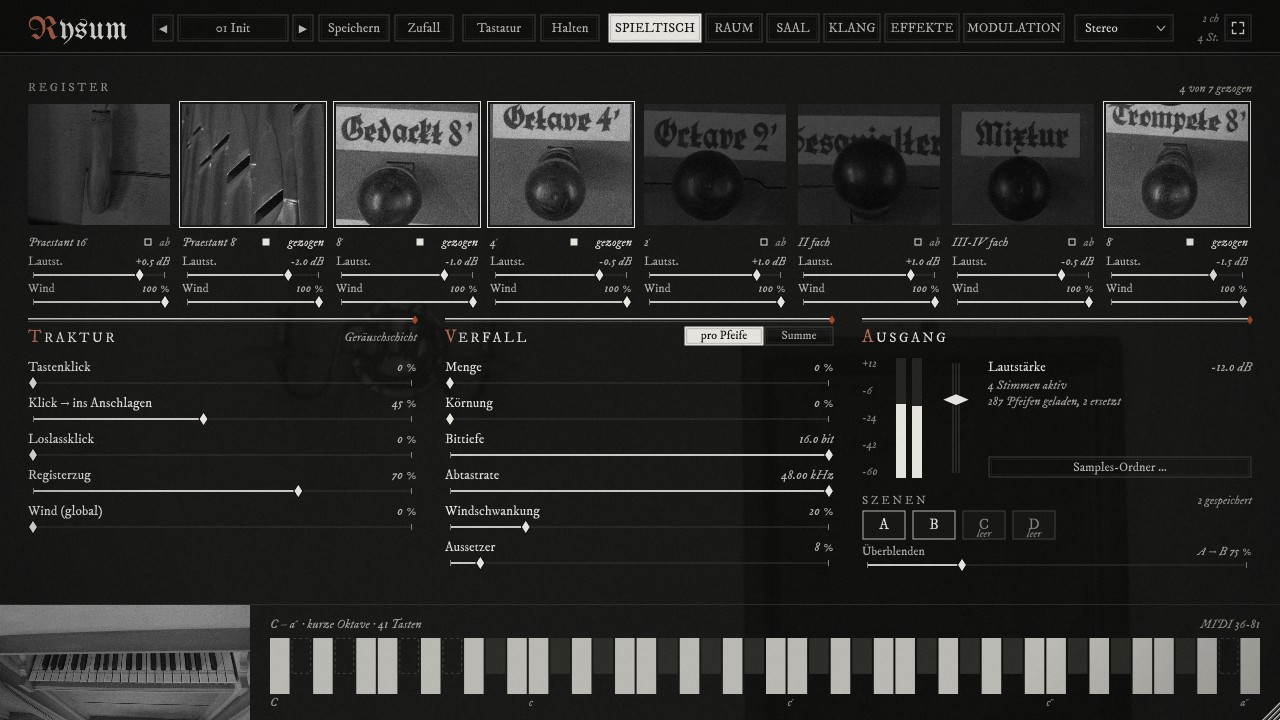
\includegraphics[width=\linewidth]{screens/ui_spieltisch.jpg}
\caption{\ui{Spieltisch} (console). Top: the stops as photographs of the real stop knobs -- click to pull or
push -- each with volume and wind. Middle: \ui{Traktur} (key click, click into the attack, release click,
stop pull, global wind), \ui{Verfall} (amount, grain, bit depth, sample rate, wind wobble, dropouts; per pipe
or sum) and \ui{Ausgang} (meters, master volume, voice count, library status, and the scene buttons \ui{A}--\ui{D} with \ui{Überblenden}). Bottom: a photograph of the
keyboard and a playable keyboard strip showing the short octave.}
\label{fig:ui1}
\end{figure}

\begin{figure}[p]
\centering
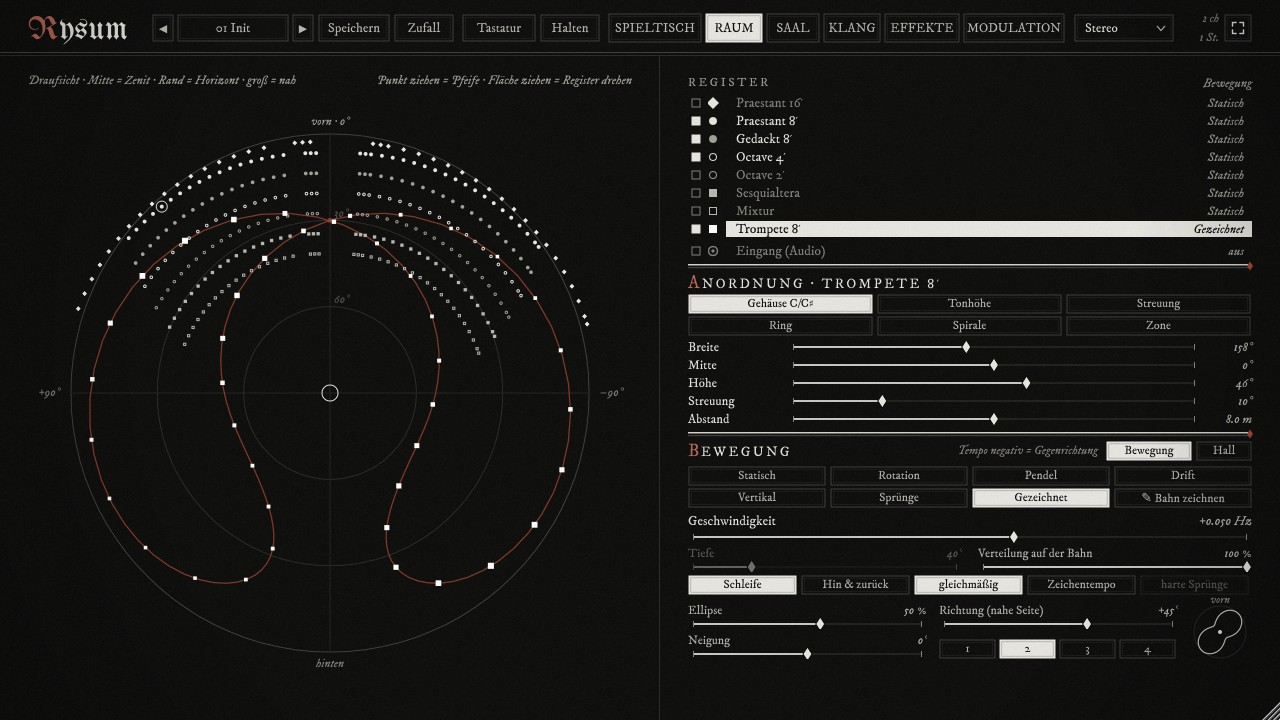
\includegraphics[width=\linewidth]{screens/ui_raum.jpg}
\caption{\ui{Raum} (space). Left: top view of all pipes of all stops (centre = zenith, rim = horizon, size =
nearness); here the Trompete follows a drawn path (red). Right: stop list with motion modes, layout
generators, and the tabs \ui{Bewegung} (motion, speed, path options, ellipse with its little orbit preview)
and \ui{Hall} (impulse response).}
\label{fig:ui2a}
\end{figure}

\begin{figure}[p]
\centering
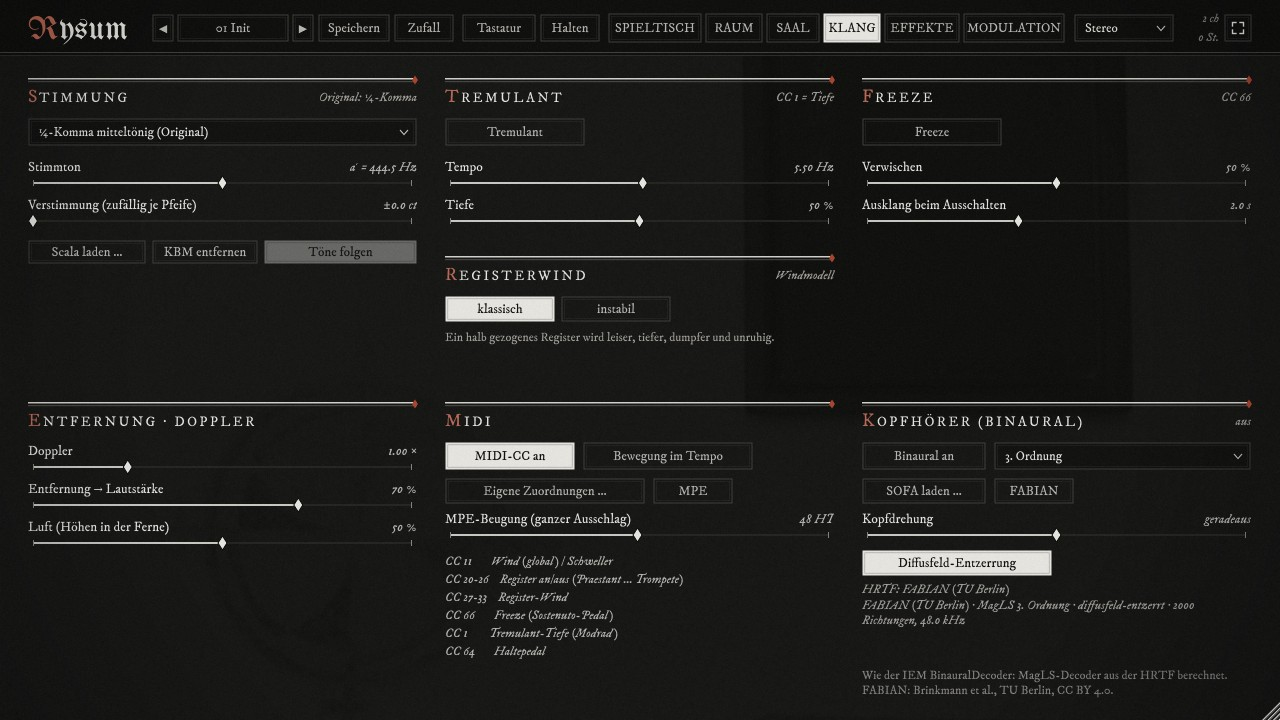
\includegraphics[width=\linewidth]{screens/ui_klang.jpg}\\[0.6em]
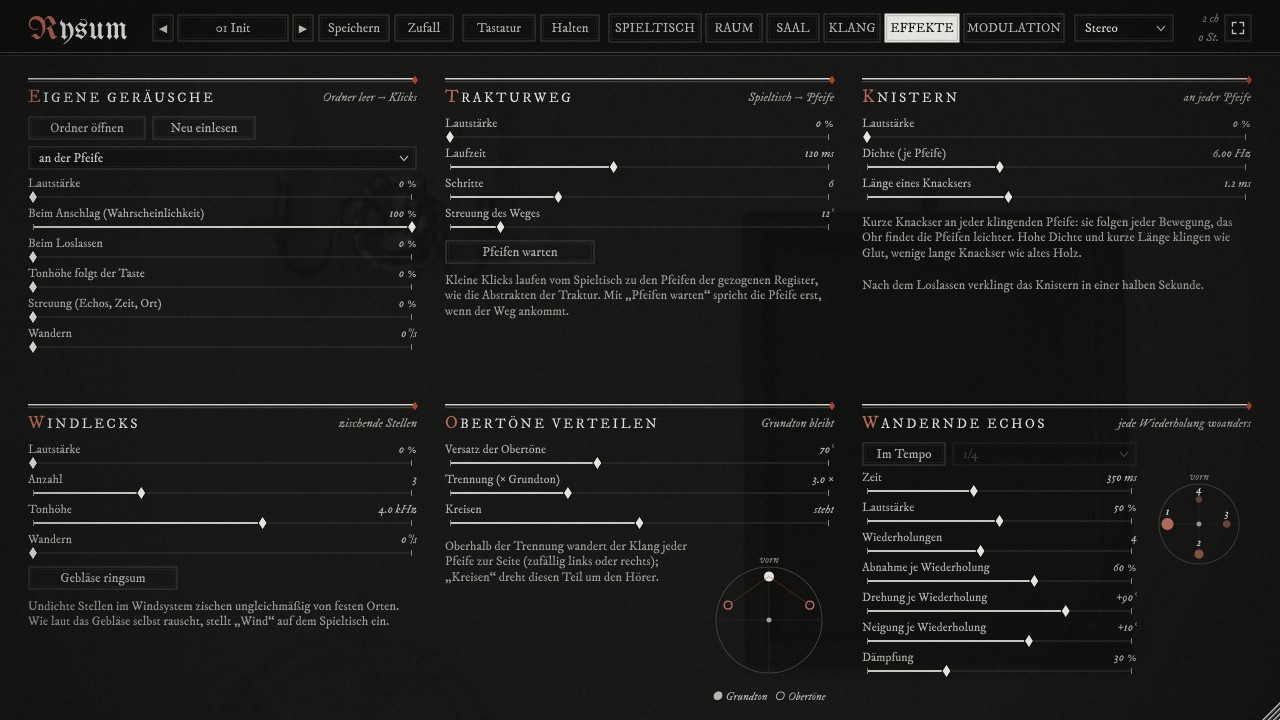
\includegraphics[width=\linewidth]{screens/ui_effekte.jpg}
\caption{Top: \ui{Klang} (sound) -- tuning (with Scala/MTS-ESP), tremulant, freeze, \ui{Registerwind}
model, distance and Doppler, MIDI options, and binaural headphone rendering. Bottom: \ui{Effekte}.}
\label{fig:ui2}
\end{figure}

\begin{figure}[p]
\centering
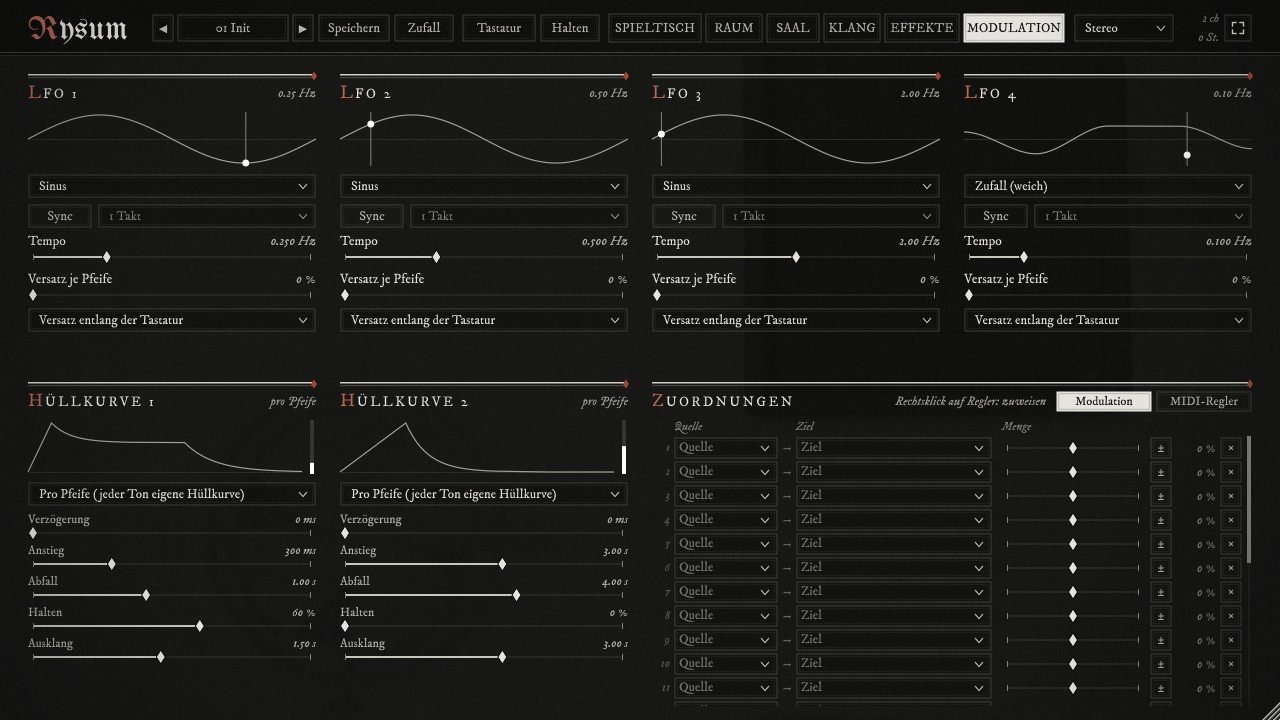
\includegraphics[width=\linewidth]{screens/ui_mod.jpg}\\[0.6em]
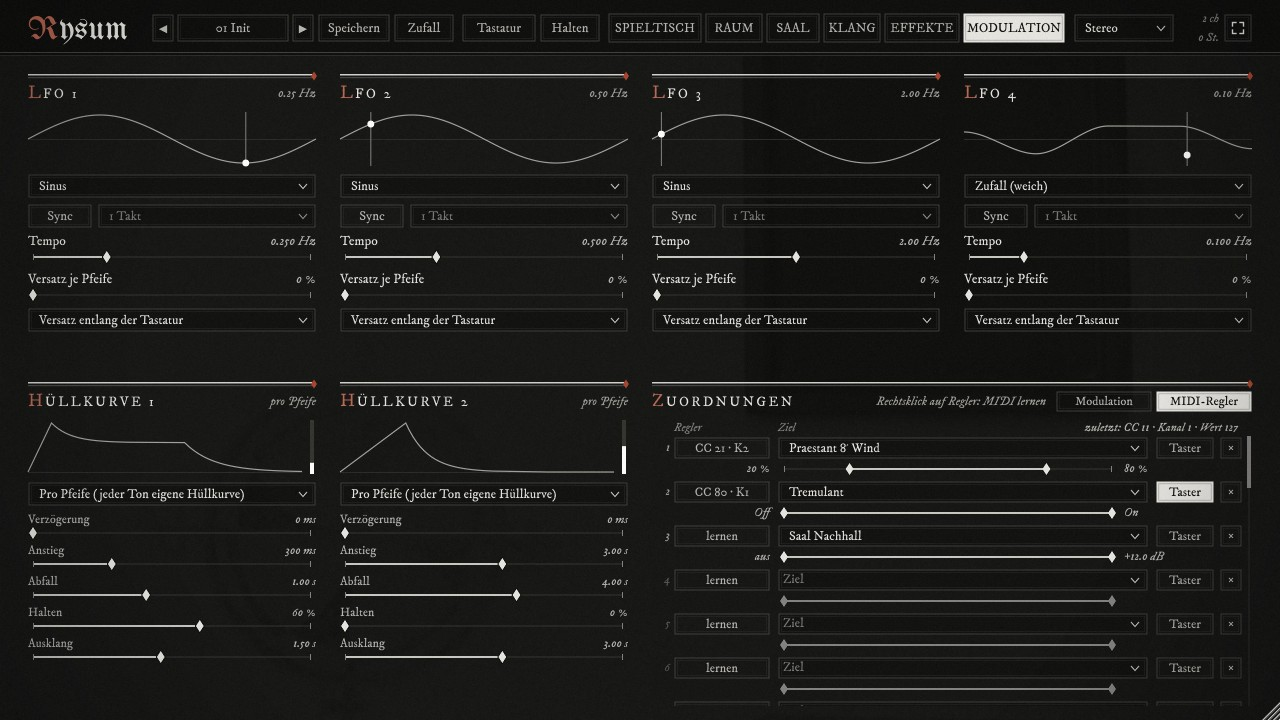
\includegraphics[width=\linewidth]{screens/ui_midi.jpg}
\caption{\ui{Modulation}. Four LFOs with shape display (the dots show where each key's pipe is on the wave),
two envelopes, and the routing matrix. Bottom: the \ui{MIDI-Regler} tab with learned controllers, ranges and
\ui{Taster} mode.}
\label{fig:ui3}
\end{figure}

\begin{figure}[p]
\centering
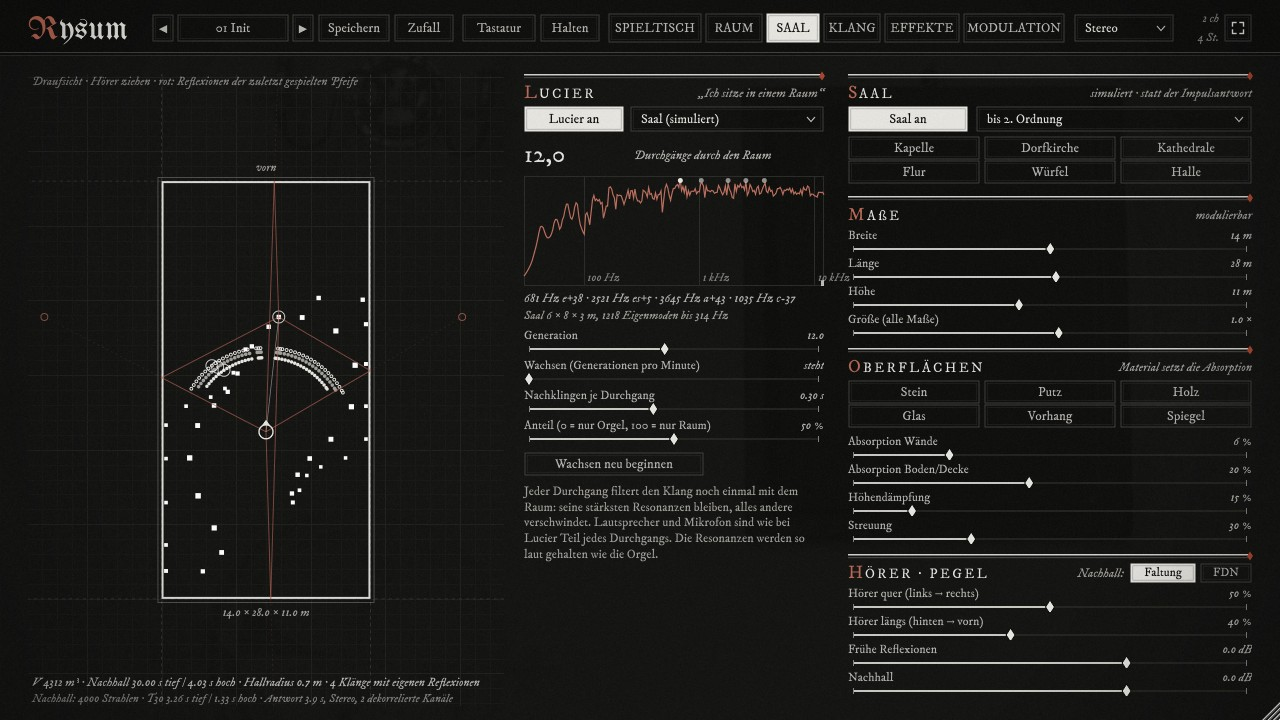
\includegraphics[width=\linewidth]{screens/ui_saal.jpg}
\caption{\ui{Saal} (hall). Left: plan view of the simulated shoebox, with the listener and the reflections of the
most recently played pipe in red. Middle: the \ui{Lucier} controls -- room, generation, growth, damping and
mix -- with the response of the room after $n$ passes and its strongest resonances. Right: room size and
presets, surfaces, the listener's position and the reverberation settings.}
\label{fig:uisaal}
\end{figure}

\begin{figure}[p]
\centering
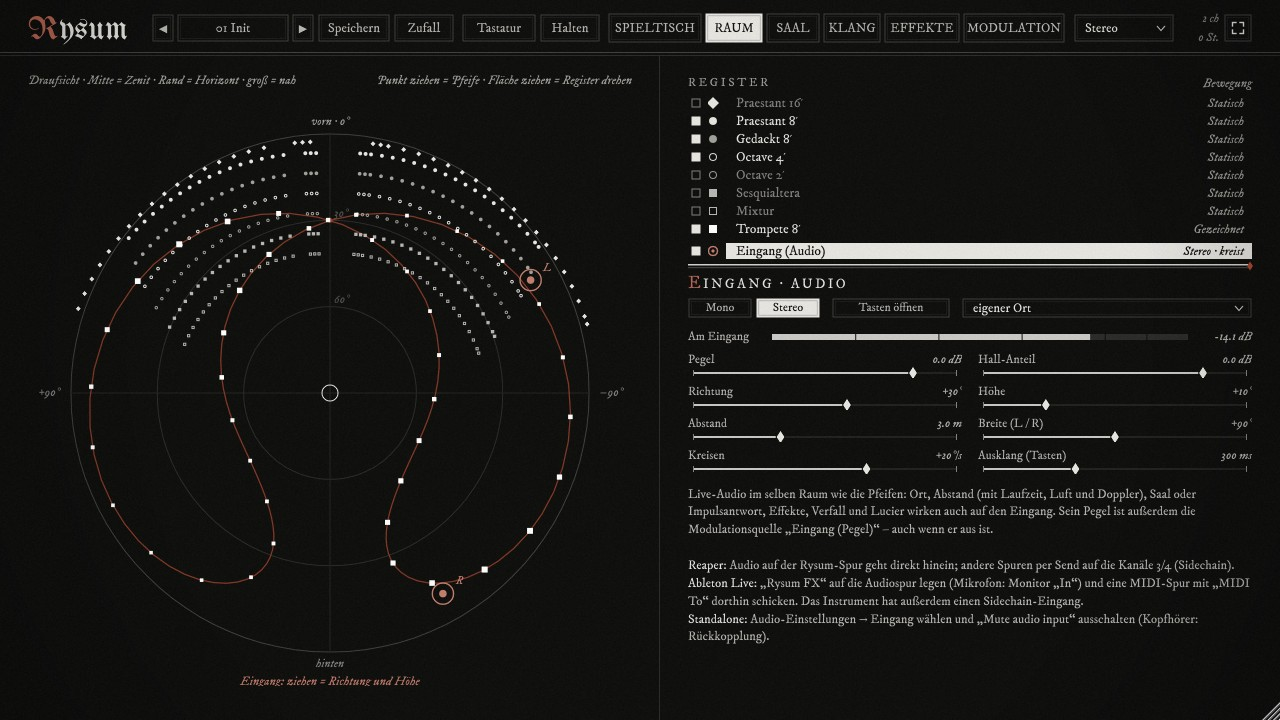
\includegraphics[width=\linewidth]{screens/ui_eingang.jpg}
\caption{\ui{Raum} with the audio input open (last row of the register list). The top view shows the two channels
of a stereo input (red, L and R) circling the listener among the pipes; below, mono or stereo, \ui{Tasten
öffnen}, the input meter, level, direction, height, distance, width, spin and release.}
\label{fig:uieingang}
\end{figure}

\begin{figure}[p]
\centering
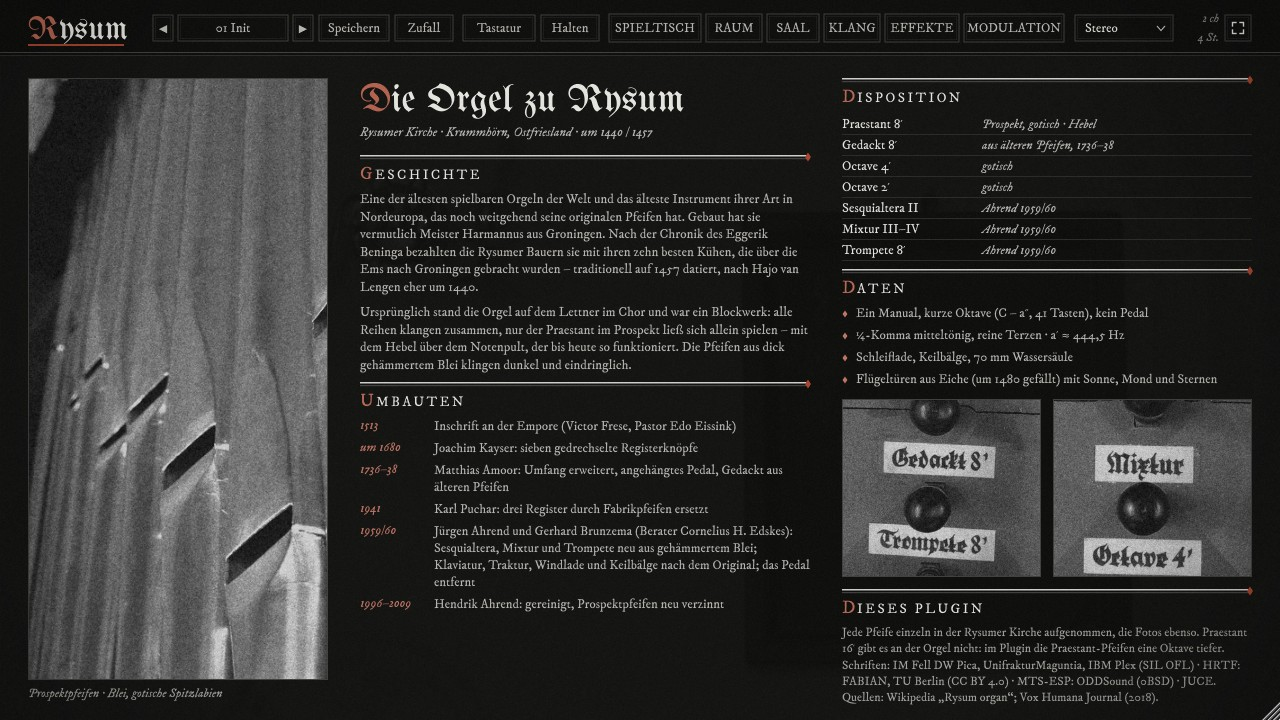
\includegraphics[width=\linewidth]{screens/ui_orgel.jpg}
\caption{The organ page, opened by clicking \ui{Rysum}: history, stops and disposition, the origin of the
pipes, and photographs of the stop knobs and the Praestant case.}
\label{fig:uiorgel}
\end{figure}


% =====================================================================
\section{Verification}
\label{sec:verification}
% =====================================================================

The repository contains two test programs that run without a host. \fn{RysumRenderTest} renders MIDI scenes
through the engine to WAV files and checks the mathematics of every subsystem; \fn{RysumUiSnapshot} renders
every page of the interface to PNG (the screenshots in this document were produced with it) and checks, among
others, typed-value parsing and the IR path. In addition the plug-in passes \emph{pluginval} at strictness
level 8. Table~\ref{tab:tests} lists a selection of results from a run made for this document on a Linux
machine (two CPU cores, so real-time factors are conservative). The run of 1 November 2026 covers the features added since the previous version (Lucier mode, audio input, scenes, dice, MPE). It reports 167 passing checks and 22 failures; the failures are listed below and are not included in the table.

\paragraph{Run of 15 November 2026.} For this version the three test runs were repeated on the author's Windows desktop (AMD Ryzen~5 2600X, six
cores; Radeon RX~6700~XT) with the complete sample library (287 pipes, of which only Gedackt f and f$\sharp$ are substituted, \S\ref{sec:future}),
at commit \code{44b5ef0}. Their logs are kept with this document.
\begin{itemize}
  \item \fn{RysumRenderTest}: \textbf{375 checks, all passed}, in about a minute and a half.
  \item \fn{RysumUiSnapshot}: \textbf{all 67 checks passed}; besides, every one of the 175 factory patches was played and measured (all play,
        the patches with a built-in room load it, the sixteen patches of set~17 knock), and the hand-played patches of set~14 respond to velocity,
        mod wheel and pitch wheel.
  \item \fn{RysumUiSnapshot} with \code{RYSUM\_ONLY\_WALK} (the 3D view, \S\ref{sec:walk}): \textbf{46 checks, all passed}
        (Table~\ref{tab:tests2}).
\end{itemize}
\emph{pluginval} was not run again. The 22 failures of 1 November are discussed below. Some results of Table~\ref{tab:tests} are the same in
both runs to the printed digits (the binaural band errors of 2.28, 0.98 and \SI{0.81}{dB}, the Lucier contrasts, the ray tracer against Eyring);
others differ a little (the diffuse-tail energies, the wall reflection's delay and angle, which are now \SI{4.104}{ms} and \SI{38.4}{\degree}) or
much (the speed of the decoders, measured on a different machine).

\begin{table}[!htb]
\centering\small
\begin{tabularx}{\linewidth}{@{}lX@{}}
\toprule
Subsystem & Result \\
\midrule
AmbiX encoder & SN3D orthogonality up to order 5, max.\ error $1.2\times10^{-4}$; ACN\,4 and ACN\,6 match the closed forms; stereo +90° = left, centre equal power \\
Binaural (MagLS) & band error vs.\ measured FABIAN HRTFs: 2.28\,dB rms (order 1), 0.98\,dB (order 3), 0.81\,dB (order 5); worst ITD error \SI{15}{\micro s} at order 3; decoder equals direct convolution to \SI{-133}{dB}; diffuse field per ear \SI{-3.07}{dB}; 44.1/96\,kHz designs within 0.04\,dB; 5th-order decoder $12\times$ real time \\
IR convolver & direct sound of a rotated IR found; early reflections turn with the pipe; diffuse tail energies $\times(2l+1)/W$ = 1.05, 1.04, 1.00 for $l=1,2,3$; $W$/$Y$ correlation $-0.04$ \\
Motion & all continuous modes move without steps (max.\ \SI{0.22}{\degree} per update); jumps hold still between jumps; ellipse near/far distances and tilt as specified; drawn paths, spread and ping-pong correct; hard vs.\ glided jumps at 150\,Hz: \SI{-33}{dB} vs.\ \SI{-58}{dB} energy above 8\,kHz \\
Unstable wind & (the model before 14 November) full wind bit-identical to the classic model (Praestant, Gedackt, Trompete); at a steady 22\,\% wind the edge tone of c′ is \SI{2399}{Hz} with \SI{2.3}{ct} spread; struck twice: 2402/2396\,Hz; falling wind: \SI{3360}{Hz} $\rightarrow$ \SI{2089}{Hz} and \SI{9}{dB} quieter; neighbouring pipes differ \\
Scala & 31-EDO parsed, one step 38.71\,ct, $a'$ = 444.5\,Hz on note 69 (the default of that run; changed since, \S\ref{sec:tuning}); ratios and \code{.kbm} with unmapped keys and reference frequency; broken files refused \\
Effects & echoes from successive directions; upper partials displaced while $W$ level is kept; crackle located at the pipe and gone after release; leaks are point sources; diffuse blower (directedness 0.007) at the same level; pipes wait for the tracker path \\
\ui{Saal} & ray tracer vs.\ Eyring in a diffuse \SI{10}{m} cube: 1.22\,s vs.\ 1.20\,s; hard corridor with dead floor/ceiling: 4.28\,s vs.\ 0.33\,s (Eyring fails, as expected); wall reflection delay \SI{4.083}{ms} (expected 4.091) from \SI{38.63}{\degree} (expected 38.66); reflections after 40\,min of running identical to a fresh start; FDN after 12\,min identical; tail swapped while playing: max.\ \SI{0.13}{dB} level difference; tail impulse response dense (99.9\,\% of peaks within \SI{10}{dB} of the local median) \\
Lucier mode & contrast of the strongest resonances over the organ: \SI{6.7}{dB}, \SI{26.7}{dB}, \SI{80.6}{dB} and \SI{203.7}{dB} at generations 1, 4, 12 and 30; the strongest resonance at generation 30 is \SI{681}{Hz}; the wet sound is about as loud as the organ; switched off, the organ returns unchanged; an impulse-response file is read, resampled and trimmed \\
Audio input & a mono source at $+90\,°$ is heard only on the left (\SI{-4.3}{dB}, right silent); a stereo input fed on one side only sounds on that side; in Ambisonics a source at $+90\,°$ gives $\langle W,Y\rangle/\langle W,W\rangle=1$; a source \SI{10}{m} away arrives after 1329 samples (1329 expected); silent without keys, \SI{-4.2}{dB} with a key held; its loudness responds to noise (0.73) and not to silence (0) \\
Scenes and dice & a scene at 25\,\% and one at 75\,\% of the morph control differ by \SI{-7}{dB} and \SI{-1}{dB} in volume; the master volume is unchanged and the scenes are kept in the state; a roll of the dice changes the sound, keeps the master volume and is undone exactly \\
MPE & pressure on a note channel changes only its own note (\SI{12}{dB} against \SI{0}{dB}); \textbf{pitch bend fails} (see below) \\
Performance & see Table~\ref{tab:bench} (from \fn{RysumBench}; the older render-test figures of $6\times$ and $2.1\times$ real time predate the optimisation and were not repeated) \\
\bottomrule
\end{tabularx}
\caption{Selected results of the offline render test (run of 1 November 2026).}
\label{tab:tests}
\end{table}

Earlier development runs with the complete sample set reported the pitch of all tunings within $\pm3$\,ct of
their targets, free tuning within $\pm5$\,ct, MTS SysEx within \SI{-0.3}{ct} and the FDN tail level within
$\pm\SI{0.5}{dB}$ of the convolution tail. The run of 1 November 2026 did not reproduce these values. It used
substitute pipes for 95 of the 287 recordings (\S\ref{sec:recording}) and reported the following failures:
\begin{itemize}
  \item \textbf{Pitch and temperament}: six meantone checks, the 31-EDO, just-intonation, harmonic-series,
        Maqam Rast and Bohlen--Pierce tunings, and both free-tuning pitch checks. The Praestant at $a'$ and its
        16$'$ partner return negative frequencies (for example \SI{-1245}{Hz}) at 44.1, 48 and 96\,kHz, so the
        pitch measurement or the sound itself is wrong. This has not been traced.
  \item \textbf{MPE}: a bend of $+2$ semitones on a note channel is measured as \SI{6826}{ct} instead of
        \SI{200}{ct}, and with MPE off the measured bend is NaN rather than zero.
  \item \textbf{Modulation}: the pitch-wheel source, the LFO-to-pitch route (expected \SI{48}{ct}, measured
        \SI{243}{ct}) and the per-pipe envelope-to-distance route.
  \item \textbf{Effects and room}: the tracker ticks do not run from the console to the pipe; the FDN decay time
        is \SI{2.21}{s} instead of \SI{3.10}{s}; the FDN tail is \SI{10.6}{dB} louder than the convolution tail.
\end{itemize}
The UI snapshot tool, run with the same samples, reported one further failure: the MTS SysEx tuning sent note 69
at \SI{603.5}{Hz} instead of \SI{466.2}{Hz}, \SI{447}{ct} off.

\paragraph{The failures of 1 November in the run of 15 November.} Every one of these checks passes in the new run, with the complete samples:
\begin{itemize}
  \item \textbf{Pitch and temperament}: the Praestant at $a'$ measures \SI{443.7}{Hz} at 44.1, 48 and \SI{96}{kHz} (\SI{-3.0}{ct} from meantone; the
        16$'$ partner \SI{-2.6}{ct}, the Gedackt f \SI{-3.0}{ct}); 31-EDO, just intonation, the harmonic series, Maqam Rast and Bohlen--Pierce lie within
        \SI{3}{ct} of their targets, free tuning within \SI{3.3}{ct}. The negative frequencies of 1 November do not occur.
  \item \textbf{MPE}: a bend of $+2$ semitones on a note channel measures \SI{196.9}{ct}, and with MPE off a bend leaves the note unchanged.
  \item \textbf{Modulation}: the pitch wheel bends by \SI{197.2}{ct}, LFO to pitch gives \SI{48.3}{ct} (expected 48), and the per-pipe envelope
        moves the distance.
  \item \textbf{Effects and room}: the tracker ticks run from the console (\SI{-5}{\degree}) to the pipe (\SI{-36}{\degree}); the FDN tail lies
        \SI{0.44}{dB} from the convolution tail. Its measured decay is \SI{2.44}{s} against the traced \SI{3.10}{s} (the convolution's
        \SI{3.21}{s}); the check asks for less than 25\,\% deviation and passes at 21\,\%, so the FDN still decays about a fifth faster than the room
        it stands for.
  \item \textbf{MTS SysEx} (UI tool): note 69 sounds at \SI{466.24}{Hz}, \SI{0.3}{ct} from the target.
\end{itemize}
Why they failed then is not known with certainty. The run of 1 November used a Linux machine and a sample set in which a third of the pipes were
substitutes, and the tuning code was reworked between the two runs (the calibrated sample pitch, \S\ref{sec:tuning}); the new run shows that the
code as it stands passes these checks with the real samples, not which of these changes cured them.

\begin{table}[!htb]
\centering\small
\begin{tabularx}{\linewidth}{@{}lX@{}}
\toprule
Part & Result (run of 15 November 2026) \\
\midrule
Walking & after \SI{0.1}{s} \SI{0.06}{m} (at once it would be 0.16), after \SI{1}{s} \SI{1.42}{m}, coasting \SI{0.24}{m}; a jump \SI{0.81}{m} high, landing after \SI{0.72}{s}; walked \SI{3.2}{m}, the engine's listener \SI{3.1999}{m} \\
Materials & the cross finds the right wall; $T_{30}$ all stone \SI{12.99}{s}, one wall a curtain \SI{3.23}{s} (Eyring \SI{3.25}{s}), all walls curtains \SI{1.30}{s} \\
Room models & each of the six built-in rooms loads (724--1466 triangles), the Saal takes its size and one can walk in it; the first flight of the stair tower is climbed to \SI{4.20}{m}; in the crypt no pipe enters a column or wall in \SI{6.4}{s} of flight and fall (six started inside one and passed out); walking into a pillar stops at \SI{2.70}{m} (the pillar begins at 3.0); a pipe behind it is \SI{6.3}{dB} quieter and low-passed at \SI{1275}{Hz}; $T_{30}$ through the model \SI{2.49}{s}, the bare Saal \SI{2.80}{s} \\
Light & mean brightness 0.319 with light, 0.134 dark with a chord, 0.054 dark and silent; a lantern 0.121 $\rightarrow$ 0.164 \\
Hands & shockwave: \SI{4.99}{m} $\rightarrow$ \SI{6.49}{m}; held still \SI{6.488}{m} $\rightarrow$ \SI{6.488}{m}; called home \SI{4.98}{m}; a click on the pipe under the cross knocks once; carried \SI{3.00}{m} ahead, thrown \SI{2.46}{m}, then it stays (\SI{0.12}{m} in \SI{2}{s}); a clap \SI{-41.4}{dB}, over after half a second \\
More hands & a pinned pipe moves \SI{0.000}{m} while a shockwave drives the others \SI{2.69}{m}; paused, nothing moves, afterwards \SI{4.25}{m}; slow motion \SI{0.37}{m} where otherwise \SI{1.33}{m}; a pipe held sounding adds a voice and lets it go; a whirlwind moves the pipes \SI{2.89}{m} on average \\
Arranging & a row of 12 chosen pipes within \SI{0.02}{m} of their places, low notes on the left; a sweep knocks 20 pipes once each; undo within \SI{0.03}{m}; F1 restores a layout within \SI{0.04}{m} and the layout is in the project; the magnet draws pipes from \SI{2.96}{m} to \SI{0.88}{m} of its point \\
The room & Ctrl+wheel $1.00\rightarrow1.50\rightarrow1.00$; lanterns kept with the project, Shift+K and Ctrl+K remove; the ears stay behind and come back \\
Illusions & \ui{Selbstspiel} at most 34 voices; \ui{Wachsen \& Brechen} a pipe of half the length has twice the zero crossings, 187 breaks in \SI{4}{s}, all back when switched off; \ui{Flüstern} \SI{16.6}{dB} between the ears at \SI{15}{cm}, a carried pipe at \SI{20}{cm} \SI{13.9}{dB}, through the plug-in (binaural) \SI{3.7}{dB} $\rightarrow$ \SI{12.7}{dB}; \ui{Zeit als Entfernung} a second back exactly, \SI{4.9}{s} back through the plug-in, then the present again; \ui{Hörraum} \SI{2.63}{s} $\rightarrow$ \SI{10.52}{s} at four times the size \\
Audience & the page is served with its font and photograph and nothing else; a tap knocks once, a second within \SI{90}{ms} does not; a swipe drives the pipes from \SI{4.99}{m} to \SI{7.26}{m}; a drag to the right blows them \SI{1.8}{m} to the right; an idle connection holds nothing up; a second instance takes the next port; switched off, the port is closed \\
Unstable wind & (the model of 14 November) full wind still bit-identical to the classic model; at a steady 22\,\% wind the mouth tone of c′ lies around \SI{759}{Hz} and later \SI{761}{Hz} (\SI{5.1}{ct}), its strongest line \SI{17.7}{dB} above its surroundings (a band, not a whistle); struck twice: 760/763\,Hz; falling wind: \SI{776}{Hz} $\rightarrow$ \SI{530}{Hz} and \SI{8.7}{dB} quieter; e′ at the same wind \SI{1422}{Hz}; at 12\,\% wind the energy above \SI{2.5}{kHz} rises from $-106$ to \SI{-69}{dB} (Praestant) \\
Other & immersive view fills the window and hides the controls; 368 buttons can be assigned to MIDI, a CC flips a page, a note a switch, a held button follows \\
\bottomrule
\end{tabularx}
\caption{Selected results of the 3D view's checks and of the new parts of the engine test (run of 15 November 2026; all passed).}
\label{tab:tests2}
\end{table}

\paragraph{Run of 18 November 2026.} For this version the test programs were run again on the same desktop, at commit \code{8a9cbe5} with
the complete samples (\fn{RysumUiSnapshot} with the change to the tool described below, committed together with this document); the logs are kept
with this document as well.
\begin{itemize}
  \item \fn{RysumRenderTest}: \textbf{384 checks, all passed}, among them the new ones for the long room, the dispersion of the Saal and the effects
        of a single stop (Table~\ref{tab:tests3}).
  \item \fn{RysumUiSnapshot}: \textbf{85 checks, all passed}, with all 181 patches of the patch folder (the 175 factory patches and six of the author's own)
        played again; the checks of the \ui{Verlauf}, the
        pieces and the \ui{Summe} are new. In the first run one new check failed: \enquote{a lane pulls a stop} found the organ already sounding before
        the lane pulled the stop. The check had only been run with \code{RYSUM\_QUICK}, which skips the factory patches; in the full run the last factory patch
        played was still loaded and sounded with the held key although every stop was pushed in. The tool now gives back the state it had before playing the factory patches, so the
        later checks start from the same state in both modes, and the check passes; the plug-in was not changed. (A first attempt that loaded the
        Init patch instead made another check fail, which expects that earlier state.)
  \item \fn{RysumUiSnapshot} with \code{RYSUM\_ONLY\_WALK}: \textbf{48 checks, 47 passed}. The one failure is the walking check (after
        \SI{0.1}{s} \SI{0.147}{m}, after \SI{1}{s} \SI{3.55}{m}, coasting \SI{0.60}{m}, against 0.06, 1.42 and 0.24 in the run of 15 November): every
        distance is 2.5 times the expected one, and the walking pace stored for this computer (\fn{Steuerung.xml}, \S\ref{sec:walk}) was set to
        $\times2.5$, which the tool reads like the plug-in. The check does not yet fix the pace for itself; it was not run again with the pace at
        $\times1$.
  \item \fn{RysumUiSnapshot} with \code{RYSUM\_ONLY\_CONCERT}: \textbf{20 checks, 19 passed} in the first run. The failure: the player's audio input
        and a note played at the same moment arrived \SI{2.94}{ms} apart at the listener, where the check allows \SI{2}{ms}. In two further runs the
        same check passed (\SI{0.00}{ms} and \SI{0.02}{ms}), so it is intermittent; its cause has not been found.
  \item \fn{RysumVoxTest} (the \ui{Vox humana} against PyTorch) was \emph{not} run for this document: it needs reference vectors written by
        the Python side of NeuralRysum, which are not on this computer. Its figures in \S\ref{sec:vox} are those of the model report
        \citep{neuralrysum2}.
\end{itemize}

\begin{table}[!htb]
\centering\small
\begin{tabularx}{\linewidth}{@{}lX@{}}
\toprule
Part & Result (run of 18 November 2026) \\
\midrule
Long room & reverberation time \SI{30}{s} (low band) and \SI{9.18}{s} (high band) in a response of \SI{12.12}{s}: steepest fall \SI{1.62}{dB} per \SI{50}{ms} while above \SI{-70}{dB}, \SI{-76.9}{dB} \SI{0.15}{s} before the end (no cut) \\
Dispersion & a click through the Saal: \SI{250}{Hz} and \SI{1}{kHz} arrive \SI{0}{ms} after \SI{4}{kHz} dry and with the reflections; with \ui{Eis} \SI{0.6}{ms} and \SI{10}{ms} later (the measure sees the ice) \\
A stop's own effects & level spread (5--95\,\%) of the stop with its own tremulant \SI{5.51}{dB}, of another stop \SI{0.97}{dB} as without; share above \SI{6}{kHz} 0.0021 $\rightarrow$ 0.0071 with its own crackle; its leaks \SI{-22.4}{dB} while drawn, silent when pushed in; speed spread: two pipes \SI{27.7}{\degree} apart drift to \SI{97.4}{\degree} in \SI{4}{s}, switching it on moved a pipe \SI{0.84}{\degree} \\
\ui{Summe} & bell \SI{+6}{dB} at \SI{1}{kHz}: \SI{+6.00}{dB}; low shelf \SI{-6}{dB}: \SI{-5.96}{dB} at \SI{30}{Hz}, \SI{0.03}{dB} at \SI{15}{kHz}; compressor \SI{-20}{dB}, 4:1: \SI{0}{dBFS} $\rightarrow$ \SI{-14.93}{dB} \\
\ui{Verlauf} & own clock 1.00267 beats per second at 60 BPM, 2.00533 with a tempo lane at 120 BPM; A--B from beat 1 to 3; chance 50\,\%: 100 of 200 passes moved; an LFO swings $0.30\dots0.70$ around the curve's 0.50; a lane pulls a stop: RMS 0.0039 $\rightarrow$ 0.091; spreading front: near pipes 0.75 while far ones are still at 0.50, inwards the other way round; host clock stopped and playing; mouse: markers, A--B, a Euclidean fill of 5 hits in 8; all six pieces load \\
3D view & AmbiX out: a held chord at \SI{12.7}{\degree}, with the head turned \SI{90}{\degree} to the left at \SI{-77.3}{\degree} (turned by \SI{-90.0}{\degree}); \ui{Alles zurücksetzen}: model, lanterns, pose and parameters as in a new instance \\
\ui{Konzert} & the listener's controls equal the player's (0 differ) and the \ui{Verlauf} comes along; two notes \SI{100}{ms} apart are \SI{100.00}{ms} apart at the listener; the \ui{Verlauf} clock trails by 0.193 beats and the motion by 0.096 cycles (expected 0.2 and 0.1); a pipe thrown \SI{6.29}{m} flies within \SI{0.018}{m} of the player's; a listener's carried pipe follows its hand; a late listener hears the held chord; the listener's own setup comes back \\
\bottomrule
\end{tabularx}
\caption{Selected results of the checks of the parts added since 15 November (run of 18 November 2026; all of these passed).}
\label{tab:tests3}
\end{table}

\paragraph{What the runs do not cover.} The tests drive the engine and the interface without a host, a mouse, a phone or a screen. Not covered are:
setting a pipe down with the right button (the test tool cannot hold a pipe as the mouse does); a real mouse (the middle button, the held click,
Alt and Ctrl combinations, which a host may take for itself); the graphics card's picture on any card but one (the comparison mode was run on the
author's card); the phone page on real phones and with many phones at once (the checks reach it through the computer's own address); and the CPU figures of \S\ref{sec:perf},
which are single measurements on the author's computer. Of what was added since 15 November, not covered are: a concert between two computers
(player and listener ran on one computer, through its own address) and with several listeners on a real network; the \ui{Vox humana} played by a
microphone in a host, and listening tests of it (its CPU figures in \S\ref{sec:vox} come from \fn{RysumVoxRender} and the model report, not from this
run); the \ui{Verlauf} in hosts other than the standalone and the test tool.

% =====================================================================
\section{Limitations and future work}
\label{sec:future}
% =====================================================================

\begin{itemize}
  \item \textbf{New recordings.} The second session of 30~October~2026 brought a clean wind loop, three clap
        responses of the church and 104 further key clicks (\S\ref{sec:recording}). What was planned beyond that is
        still open: all stops again with the keys in physical order, stop pulls, room noise, and Ambisonic impulse
        responses of the church (the claps are stereo).
  \item \textbf{A recorded wind model.} Wind starvation is still synthetic: every pipe recorded while its stop is
        slowly pushed in and pulled out, plus fixed intermediate positions, would let the model of \S\ref{sec:windchaos}
        be replaced or checked against the real organ.
  \item \textbf{Gedackt f and f♯} are currently replaced by neighbouring pipes and need to be re-recorded.
  \item \textbf{Hosts.} The binaural mode and the computer keyboard have so far been tested mainly in Reaper
        and the standalone application; practical tests in Ableton Live are outstanding.
  \item \textbf{Rooms.} The floor plans of \S\ref{sec:plans} have vertical walls and a flat ceiling; vaults, domes
        and galleries, and the exact room modes of an arbitrary plan (needed by the Lucier mode), are not modelled.
        Four rooms at a time are the limit. An imported model gives the direct sound (round its edges) and the late reverb, but the early reflections still follow the shoebox of the Saal.
  \item \textbf{Reference tone and calibration.} The pitch correction and the DSF tone were written to compare the samples by ear; I have not
        compared them with a measurement, and the reference tone's error curve (Fig.~\ref{fig:dsf}) is that of the formula, not of the finished audio.
  \item \textbf{Transaural.} The cancellation needs a listener in the middle between two symmetric loudspeakers; the reduction
        figures of \S\ref{sec:transaural} are those of the HRTF set itself, not measurements in a room.
  \item \textbf{MPE.} The pitch bend now passes the offline test (\S\ref{sec:verification}), but MPE has not been tried with hardware controllers.
  \item \textbf{Audio input and Lucier mode.} Both have been tested offline and in the standalone application, not yet in Ableton Live or with live microphones. The Lucier mode damps every pass (\S\ref{sec:lucier}) so that the resonances appear within seconds; it approximates the process rather than reproducing the time course of a real re-recording.
  \item \textbf{What the tests cover.} The runs of 15 and 18~November cover the engine and the interface offline, including everything added
        since 1~November (\S\ref{sec:verification}), but not the use with the hands: a real mouse in a host, the graphics card's picture on other
        cards and drivers, real phones in numbers, a concert across several computers. Setting a pipe down has no automatic check. The tests passing say that the code does what it
        was written to do, not that it sounds as it should; that is decided by listening.
  \item \textbf{The 3D view in hosts.} Its keys (Alt, the F keys, Ctrl+Z, the middle mouse button) may be taken by a host before the plug-in sees
        them; how each host behaves has not been tried systematically.
  \item \textbf{Pipes as bodies.} A pipe has a place and a velocity but no orientation: it does not tip over or spin, so it cannot be turned by
        hand, and a falling pipe always lands upright. Pipes do not collide with each other. A broken pipe stays one pipe.
  \item \textbf{The audience.} Plain HTTP on the local network, without any login: anyone on the network can join, which suits a concert
        hall's own network and not a public one. Windows' firewall and guest networks that isolate their devices are the usual obstacles
        (\S\ref{sec:audience}).
  \item \textbf{The concert.} \ui{Konzert} works in one local network over plain TCP, without login or encryption; a player on the internet needs a
        relay server, which is planned. Player and listeners must run the same version. It has been tested with player and listener on one computer
        (the test of \S\ref{sec:verification}), not yet with many listeners on uneven networks. The Tonnetz walker, \ui{Selbstspiel}, the phone audience,
        MIDI Tuning SysEx and imported room models are not mirrored.
  \item \textbf{The \ui{Vox humana}.} The lowest octave is detected slowly (\SI{33}{ms} at C2) and sometimes an octave too high, the onset head practically
        never fires on real material, so a key repeated quickly becomes one note, and octave folding shifts bass lines up. The network knows one organ and
        one room; it was trained on the plug-in's renderings, not on new recordings, and on pipes and registrations only. Listening tests in a host, and the
        tuning of its default level and tracker settings, are still to be done \citep{neuralrysum2}.
  \item \textbf{The \ui{Verlauf}.} It is built for performing rather than for complete pieces: up to 16 lanes, the controls of the \ui{Saal}, the Lucier
        mode and the tuning have no lanes, and switches (stop knobs, buttons) sound as their lane says but do not move on screen.
  \item \textbf{Distribution.} The plug-in is currently passed to testers as a standalone executable with
        the sample folder and patches, and listeners get \emph{Rysum Konzert} as a zip with the samples; in both the samples are plain files that anyone
        can open. An installer, a protected sample archive and a decision on licensing and distribution are open.
\end{itemize}

% =====================================================================
\section{Conclusion}
% =====================================================================

\emph{Rysum} turns a fifteenth-century meantone organ into a spatial instrument. A careful preprocessing
keeps what makes the instrument specific -- its temperament, its voicing, its compass, its noises -- and
documents every automatic decision. On top of this faithful base, the engine treats each of the 287 pipes
as a moving sound source in an Ambisonic or binaural scene, with a playable room, a model of starving wind,
and tools for detuning, degrading and modulating the organ that have no historical counterpart. In its newest part the
room becomes a place to be in: the pipes can be walked among, knocked, carried, thrown and arranged by hand, in a chapel, a crypt or a stair
tower, and an audience can take part, on their phones or on computers of their own that render the organ from where each of them stands.
Curves in time let the instrument move by itself while one plays, and a neural stop trained on the plug-in's own sound lets a voice or any other
input play the organ. The result is
both a document of a specific instrument and material for new spatial music.

% =====================================================================
\bibliographystyle{plainnat}
\bibliography{refs}

% =====================================================================
\clearpage
\appendix
% =====================================================================
% Mathematical reference: the signal processing, function by function.
% Included from main.tex (% =====================================================================
% Mathematical reference: the signal processing, function by function.
% Included from main.tex (% =====================================================================
% Mathematical reference: the signal processing, function by function.
% Included from main.tex (\input{math}). Every formula here was read off the source code of
% the commit named in the text; the function names are those of plugin/source.
% =====================================================================
\section{Mathematical reference}
\label{sec:math}
% =====================================================================

The sections before describe what each part of Rysum does and why. This section goes one level deeper: it takes the
source code function by function and writes down what each one computes, term by term, and what every term is there for.
It is meant as a companion for reading the code, so the subsections follow the source files (\fn{Common.h},
\fn{Spatial.h}, \dots) in the order a signal passes through them, from the key to the loudspeaker. Where a function was
already described with its formula in an earlier section, that section is named and only what was left out is added.
Everything was read off the code of 21~November 2026 (commit \code{bfc83f3}).

\paragraph{Conventions.} $f_s$ is the host's sample rate and $n$ the sample index. Most quantities that are not audio
(positions, gains, filter coefficients) are \emph{control-rate}: they are computed once every 64 samples and held or
ramped in between; where a function runs at another rate it says so. Angles in the code are degrees; in the formulas
they are radians unless a unit is given. Azimuth $\varphi$ is measured from the front, positive to the left;
elevation $\vartheta$ from the horizon, positive upwards (the AmbiX convention). A cent is $1/1200$ of an octave, so a
shift of $c$ cents multiplies a frequency by $2^{c/1200}$. $\operatorname{clamp}_{[a,b]}(x)=\min(b,\max(a,x))$.
Decibels are converted by
\begin{equation}
  g(\mathrm{dB}) = \begin{cases} 0, & \mathrm{dB}\le -99,\\ 10^{\mathrm{dB}/20}, & \text{otherwise,}\end{cases}
\end{equation}
(\fn{dbToGain}); the cut-off at $-99$ makes the bottom of every level slider a true silence instead of
$10^{-5}$.

% ---------------------------------------------------------------------
\subsection{Random numbers (\fn{XorShift})}
\label{sec:math-rng}
All randomness that happens on the audio thread comes from one generator, Marsaglia's 32-bit xorshift
\citep{marsaglia2003xorshift}. Its state $s$ (never 0) is updated by three shift-and-exclusive-or steps,
\begin{equation}
  s \leftarrow s \oplus (s \ll 13),\qquad s \leftarrow s \oplus (s \gg 17),\qquad s \leftarrow s \oplus (s \ll 5),
\end{equation}
which walk through all $2^{32}-1$ non-zero states. A uniform number in $[0,1)$ is made from the upper 24 bits,
$u = \lfloor s/2^{8}\rfloor\cdot 2^{-24}$ (24 bits because that is the mantissa of a 32-bit float, so every value
is exactly representable), and a bipolar one as $b=2u-1$. The generator costs three shifts and has no memory
beyond one integer, so every pipe, every image source and every grain can own one. Most callers seed it
deterministically from what they belong to (a pipe's stop and key, a pass number, a channel), which is why two
renders of the same project are identical (\S\ref{sec:verification}) and why a random layout does not change when
the project is reopened.

% ---------------------------------------------------------------------
\subsection{Pitch and tuning (\fn{Common.h}, \fn{Scala.h})}
\label{sec:math-tuning}

\paragraph{The recorded pitch (\fn{meantoneHz}).} The organ stands in quarter-comma meantone at
$a' = A_4 = \SI{444.5}{Hz}$ (measured). The table $c_\mathrm{mt}[0..11]$ holds the pitch classes in cents above C
($0, 76.0, 193.2, 310.3, 386.3, 503.4, 579.5, 696.6, 772.6, 889.7, 1006.8, 1082.9$), and a MIDI note $k$ sounds at
\begin{equation}
  f_\mathrm{mt}(k) = A_4 \cdot 2^{\,\lfloor k/12\rfloor - 5 \;+\; (c_\mathrm{mt}[k \bmod 12]-c_\mathrm{mt}[9])/1200}.
\end{equation}
$\lfloor k/12\rfloor-5$ counts octaves from the octave of $A_4$ (MIDI 69 lies in octave $5$), and subtracting
$c_\mathrm{mt}[9]$ (A) anchors the table at $a'$, so $f_\mathrm{mt}(69)=A_4$ exactly. This is the pitch every sample
is assumed to have; all other tunings are expressed as a shift from it.

\paragraph{Meantone temperaments (\fn{temperamentCents}).} The family of regular meantones is generated from one
tempered fifth. With the pure fifth $F_0 = 1200\log_2(3/2) = \SI{701.955}{ct}$, the syntonic comma
$\kappa_s = 1200\log_2(81/80) = \SI{21.506}{ct}$ and the Pythagorean comma $\kappa_p = 12F_0 - 8400 =
\SI{23.460}{ct}$, the fifth is $F = F_0 - \delta$ with $\delta = \kappa_s/4$ (quarter-comma), $\kappa_s/5$,
$\kappa_s/3$, $2\kappa_s/7$ or $\kappa_p/6$. Each pitch class is then reached by a number $j$ of fifths up or down from
C and folded into the octave, $c = (jF) \bmod 1200$, with
\begin{equation}
  j = (0,\,7,\,2,\,-3,\,4,\,-1,\,6,\,1,\,8,\,3,\,-2,\,5)\quad\text{for}\quad (\mathrm{C},\mathrm{C}\sharp,\mathrm{D},\mathrm{E}\flat,\dots,\mathrm{B}).
\end{equation}
The chain runs from $\mathrm{E}\flat$ ($j=-3$) to $\mathrm{G}\sharp$ ($j=8$), so the eleven fifths inside it are
tempered and the twelfth, $\mathrm{G}\sharp$--$\mathrm{E}\flat$, takes the whole error: the wolf, $\SI{737.6}{ct}$ in
quarter-comma. Quarter-comma makes the major third pure, since $4F - 2400 = 4F_0 - \kappa_s - 2400 = 1200\log_2(5/4)$.
Well temperaments (Werckmeister III, Kirnberger III, Vallotti), Pythagorean, equal and Maqam Rast are stored as
fixed tables; just intonation 5-limit, 7-limit and the harmonic series as ratios $r$ per pitch class, converted by
$1200\log_2 r$; and 12-out-of-$N$ equal divisions ($N = 31, 19, 53$) as the step numbers $s_i$ that lie nearest to
meantone or just intonation, $c_i = 1200\,s_i/N$.

\paragraph{From temperament to shift (\fn{temperamentShift}).} The samples cannot be re-recorded, so a temperament
$c[\cdot]$ is applied as a shift per pitch class that keeps $a'$ fixed:
\begin{equation}
  \Delta_i = \bigl(c[i]-c[9]\bigr) - \bigl(c_\mathrm{mt}[i]-c_\mathrm{mt}[9]\bigr).
\end{equation}
The first bracket is where pitch class $i$ should lie relative to A, the second where it was recorded; the
difference is the transposition the sample of that pitch class needs. The shifts are small (at most about $\SI{21}{ct}$ for equal
temperament and $\SI{27}{ct}$ for Pythagorean tuning), so resampling by $2^{\Delta/1200}$ does not audibly change the
pipe's timbre.

\paragraph{Step tunings (\fn{steppedTuningCents}, \fn{makeKeyTuning}).} In the tunings where every MIDI note is one
step of size $q$ ($q = 1200/31$, $1200/19$, $50$, the Bohlen--Pierce step $1200\log_2 3/13 = \SI{146.3}{ct}$, or Carlos
Alpha $\SI{77.965}{ct}$) the target of note $k$ is $t(k) = (k-69)\,q$ cents from $a'$. In the just Bohlen--Pierce scale
the period is the tritave $3{:}1$: with $d = (k-69) \bmod 13$ and $o = \lfloor (k-69)/13\rfloor$,
$t(k) = 1200\bigl(\log_2 r_d + o\log_2 3\bigr)$ for the thirteen ratios $r_d$ ($1, 27/25, 25/21, \dots, 25/9$).
Because such a tuning can move a key by many semitones, the key does not play its own pipe. Every key $k$ is given
the recorded pipe $s^*$ whose meantone pitch lies nearest to the target,
\begin{equation}
  s^*(k) = \arg\min_s \bigl|\,1200\log_2\!\bigl(f_\mathrm{mt}(s)/A_4\bigr) - t(k)\bigr|,\qquad
  \Delta_k = t(k) - 1200\log_2\!\bigl(f_\mathrm{mt}(s^*)/A_4\bigr),
\end{equation}
so no pipe is ever transposed by more than half the distance to its neighbour (except beyond the organ's compass).
The \code{KeyTuning} record holds $s^*(k)$ and $\Delta_k$ for all 41 keys.

\paragraph{Stimmton.} The \ui{Stimmton} parameter is an additional transposition $c_S$ (stored in tenths of a cent).
Its detent at \SI{440}{Hz} is replaced by the exact value $1200\log_2(440/444.5) = \SI{-17.617}{ct}$
(\fn{effectiveStimmtonCents}), so that "440" really is 440 and not $444.5\cdot 2^{-17.6/1200} = \SI{440.004}{Hz}$.

% ---------------------------------------------------------------------
\subsection{The Ambisonics encoder (\fn{encodeAmbiX})}
\label{sec:math-encoder}
Every source in Rysum (a pipe, an image source of the room, an echo, the input) is placed by multiplying its
signal with the real spherical harmonics of its direction, up to order $L\le 5$, giving $(L+1)^2$ channels in ACN
order with SN3D normalisation and no Condon--Shortley phase (AmbiX \citep{nachbar2011ambix}):
\begin{equation}
  Y_l^m(\varphi,\vartheta) = N_l^{|m|}\,P_l^{|m|}(\sin\vartheta)\cdot
  \begin{cases}\cos(m\varphi), & m\ge 0\\ \sin(|m|\varphi), & m<0\end{cases},\qquad
  N_l^m = \sqrt{(2-\delta_{m0})\,\frac{(l-m)!}{(l+m)!}},
\end{equation}
written to channel $\mathrm{ACN} = l^2+l+m$. The normalisation $N_l^m$ is computed once into a table
(\fn{Sn3dTable}); SN3D makes the largest value of every harmonic about 1 and $Y_0^0 = 1$, so the W channel carries
the mono signal unchanged.

\paragraph{No trigonometry per order.} Because the function is called for every pipe every 64 samples and for every
image source of the room, it avoids all trigonometric calls except one $\sin/\cos$ pair for each angle. The associated
Legendre functions are built by the standard recurrences in $x = \sin\vartheta$, $c = \cos\vartheta = \sqrt{1-x^2}$:
\begin{align}
  P_m^m &= (2m-1)\,c\,P_{m-1}^{m-1}, & P_0^0 &= 1, \\
  P_{m+1}^m &= (2m+1)\,x\,P_m^m, \\
  P_l^m &= \frac{(2l-1)\,x\,P_{l-1}^m - (l+m-1)\,P_{l-2}^m}{l-m}, & l &\ge m+2,
\end{align}
(the diagonal, the first off-diagonal, and the three-term recurrence in $l$), and the multiples of the azimuth by
the angle-addition theorem,
\begin{gather}
  \cos m\varphi = \cos(m-1)\varphi\cos\varphi - \sin(m-1)\varphi\sin\varphi,\\
  \sin m\varphi = \sin(m-1)\varphi\cos\varphi + \cos(m-1)\varphi\sin\varphi.
\end{gather}
For 5th order this is 36 values for two $\sin/\cos$ pairs and about 60 multiplications. The variant
\fn{encodeAmbiXDir} takes the four cosines and sines directly, which the room simulation uses since it already has
the direction as a vector: for an image source at $(x,y,z)$ relative to the listener,
$\cos\varphi = x/\rho$, $\sin\varphi = y/\rho$ with $\rho = \sqrt{x^2+y^2}$, and $\sin\vartheta = z/r$,
$\cos\vartheta=\rho/r$, without a single trigonometric call.

\paragraph{Stereo (\fn{encodeStereo}).} For the stereo output a source is panned with the equal-power law on the
lateral component only: $p = \sin\varphi \in [-1,1]$ ($+1$ = left), $\alpha = (1-p)\,\pi/4 \in [0,\pi/2]$, and
\begin{equation}
  (g_L, g_R) = (\cos\alpha,\ \sin\alpha),\qquad g_L^2+g_R^2 = 1.
\end{equation}
Using $\sin\varphi$ instead of $\varphi$ folds front and back onto the same pan, which is what a stereo pair can
represent; the power sum is constant, so a pipe does not get louder or softer as it travels across.

% ---------------------------------------------------------------------
\subsection{Positions and motion (\fn{Spatial.h})}
\label{sec:math-motion}
A pipe's place is $(\varphi,\vartheta,d)$ with the distance $d$ clamped to $[\SI{0.5}{m},\SI{60}{m}]$. Its
\emph{base} position comes from the layout; \fn{applyMotion} turns it into the position of the moment from a
\emph{phase} $\Phi$, measured in cycles. The engine integrates the phase from the speed, $\Phi_{n+1} = \Phi_n +
v\,\Delta t$, instead of computing $v\,t$, so a change of speed never makes the pipe jump, and a negative speed runs
the same path backwards. (The per-pipe speed spread $\Phi_k = \Phi(1+\sigma r_k)+o_k$ is described in
\S\ref{sec:motion}.) With the fractional phase $\phi = \Phi - \lfloor\Phi\rfloor$:

\begin{description}[style=nextline]
  \item[Rotation] $\varphi \leftarrow \operatorname{wrap}(\varphi_0 + 2\pi\phi)$, where
    $\operatorname{wrap}$ folds an angle into $[-180^\circ,180^\circ)$.
  \item[Vertical] the pipe turns about the left--right axis (front $\to$ up $\to$ back $\to$ down). The direction is
    taken to Cartesian coordinates $x = \cos\vartheta\cos\varphi$, $y = \cos\vartheta\sin\varphi$, $z = \sin\vartheta$,
    rotated about $y$ by $a = 2\pi\phi$,
    $x' = x\cos a - z\sin a$, $z' = x\sin a + z\cos a$, and returned as $\varphi = \operatorname{atan2}(y,x')$,
    $\vartheta = \arcsin z'$.
  \item[Pendel] $\varphi \leftarrow \varphi_0 + D\sin(2\pi\Phi)$ with the depth $D$ in degrees.
  \item[Drift] three smooth random functions (below) with different seeds move azimuth, elevation and distance:
    $\varphi \leftarrow \varphi_0 + D\,\nu_1(\Phi)$, $\vartheta \leftarrow \vartheta_0 + 0.4D\,\nu_2(\Phi)$,
    $d \leftarrow d_0\,\bigl(1 + 0.4\,\tfrac{D}{180}\,\nu_3(0.7\Phi)\bigr)$. Elevation and distance move less than
    azimuth because the ear resolves them less well and a large change of distance would be heard as a change of
    level.
  \item[Sprünge] the phase plus a per-pipe offset $o\in[0,1)$ is cut into whole cycles, $i = \lfloor\Phi+o\rfloor$; a
    generator seeded from the pipe and $i$ gives three numbers $b_{1,2,3}\in[-1,1]$, and
    $\varphi = \varphi_0 + Db_1$, $\vartheta = \vartheta_0 + 0.5Db_2$, $d = d_0(1+0.6\tfrac{D}{180}b_3)$. The place
    stays constant during a cycle and changes abruptly at its end; because $o$ differs per pipe, the pipes jump at
    different moments, not all on the beat.
  \item[Gezeichnet] the pipe follows the drawn path (below) at $u = \phi + s\,\kappa$, where $\kappa\in[0,1]$ is the
    pipe's place among its stop's pipes and $s$ the spread (\ui{Verteilung}): at $s=1$ the pipes are distributed over
    the whole path like the carriages of a train. For a path drawn as \ui{hin und zurück},
    $u \leftarrow 1 - |1-2u|$, a triangle wave that runs to the end and back.
\end{description}

\paragraph{Smooth noise (\fn{smoothNoise}).} The drift needs a random function of time that is smooth, bounded and
different for every pipe, without state. It is a sum of three sines whose frequencies $f_i$ and phases $p_i$ are
drawn once from the seed ($f_1\in[0.55,1.05)$, $f_2\in[1.13,1.83)$, $f_3\in[0.31,0.61)$):
\begin{equation}
  \nu(t) = \frac{\sin(2\pi f_1 t+p_1) + 0.6\sin(2\pi f_2 t+p_2) + 0.8\sin(2\pi f_3 t+p_3)}{2.4}\in[-1,1].
\end{equation}
The frequencies are incommensurate, so the sum does not repeat audibly; the divisor $2.4 = 1+0.6+0.8$ bounds it.

\paragraph{Drawn paths (\fn{MotionPath::at}).} A drawn path is a list of up to 256 unit vectors $\mathbf{p}_i$ with
the time $u_i\in[0,1]$ at which each was drawn, so the speed of the drawing is kept. For a time $u$ the enclosing
pair $u_{i}\le u<u_{i+1}$ is found by bisection and the vector interpolated linearly,
$\mathbf{p} = \mathbf{p}_i + \tfrac{u-u_i}{u_{i+1}-u_i}(\mathbf{p}_{i+1}-\mathbf{p}_i)$, then converted back to
$\varphi = \operatorname{atan2}(p_y,p_x)$, $\vartheta = \operatorname{atan2}(p_z, \sqrt{p_x^2+p_y^2})$. Interpolating
the vectors (a chord through the sphere) instead of the angles avoids the wrong way round at $\pm180^\circ$, and
$\operatorname{atan2}$ does not need the interpolated vector to have unit length.

\paragraph{Orbit shape.} After the motion, an ellipse and a tilt can bend the orbit. With the angle from the
near side $\psi = \varphi - \varphi_e$ and $q\in\{1,2,3,4\}$ lobes,
\begin{equation}
  \vartheta \leftarrow \vartheta + T\cos\psi\cos\vartheta,\qquad
  d \leftarrow d\,\bigl(1 - e\cos\vartheta\,\cos(q\psi)\bigr),
\end{equation}
with the tilt $T$ in degrees and the eccentricity $e\in[0,0.9]$. With $q=1$ the listener sits at one focus: the
pipe comes nearest at $\psi=0$ and is farthest opposite. With $q=2$ the listener is at the centre and the pipe comes
near twice per turn, with $q=3,4$ the orbit is a rounded triangle or square. The factor $\cos\vartheta$ makes both
effects vanish towards the zenith, where azimuth has no meaning.

\paragraph{Distance (\fn{distanceGain}).} The level of a pipe falls with distance relative to the reference
distance $d_0 = \SI{4}{m}$:
\begin{equation}
  g_d = \operatorname{clamp}_{[0,4]}\Bigl(\bigl(d_0/\max(d,\SI{0.5}{m})\bigr)^{a}\Bigr),
\end{equation}
where $a\in[0,1]$ (\ui{Entfernung} $\to$ \ui{Lautstärke}) blends from no distance law ($a=0$) to the physical
$1/r$ of a point source ($a=1$). The limit of 4 ($\SI{+12}{dB}$) stops a pipe that flies through the listener from
exploding in level. Air absorption and the Doppler shift are described with the sample playback
(\S\ref{sec:math-voice}).

\paragraph{Pipe size (\fn{pipeSize}).} The length of a pipe follows its footage: an 8′ C is
$\SI{2.44}{m}$ and every semitone shortens it by $2^{-1/12}$,
\begin{equation}
  \ell = 2.44\,\tfrac{F}{8}\,2^{-k/12}\ \text{m},\qquad \ell \leftarrow \ell/2\ \text{for a stopped pipe},\qquad
  r = \ell\cdot\begin{cases}0.035,&\text{open}\\0.07,&\text{stopped}\end{cases},
\end{equation}
($F$ the footage, $k$ the key index; $\ell\in[0.12,6]$, $r\in[0.012,0.13]$). A stopped pipe sounds an octave lower
than an open one of the same length, so the Gedackt is drawn half as long and twice as wide. The 3D view draws
these sizes, and the bodies in the room use them for their collisions and their knock (\S\ref{sec:roommotion}).

% ---------------------------------------------------------------------
\subsection{Layouts (\fn{generateLayout}, \fn{tonnetzPlaces})}
\label{sec:math-layouts}
A layout writes the base position of all 41 pipes of a stop from width $W$, centre $\varphi_c$, elevation
$\vartheta_c$, spread $S$ and distance $d$. Let $\rho_k\in[0,1]$ be the rank of key $k$ by pitch ($0$ = lowest).
\begin{description}[style=nextline]
  \item[Gehäuse C/C\#] as in an organ case: the C side (even MIDI numbers) to the left, the C\# side to the right,
    bass in the middle and treble outside, $\varphi = \varphi_c \pm \tfrac{W}{2}(0.06+0.94\rho_k)$,
    $\vartheta = \vartheta_c + \tfrac{S}{2}(0.5-\rho_k)$.
  \item[Tonhöhe] a line from left (low) to right (high): $\varphi = \varphi_c + W/2 - \rho_k W$.
  \item[Streuung] uniformly random in the rectangle $\varphi_c\pm W/2$, $\vartheta_c\pm S$, with
    $d \leftarrow d(1+0.45b)$; the generator is seeded with the stop and the layout type, so the same scatter comes
    back every time.
  \item[Ring, Spirale] $\varphi = \varphi_c + 360^\circ\rho_k$ (one turn); the spiral makes two turns
    ($720^\circ\rho_k$), climbs from $\vartheta_c-S$ to $\vartheta_c+S$ and comes nearer, $d\leftarrow d(1.5-\rho_k)$.
  \item[Zone] all pipes in a small patch, $\pm0.075W$ by $\pm 0.3S$.
\end{description}

\paragraph{Tonnetz.} This layout places each key at a point $(a,b)$ of the lattice of fifths ($a$) and major thirds
($b$) \emph{of the tuning in use}. First the tuning's own fifth $F$ and third $T$ are found: for a twelve-note tuning
the medians of its twelve fifths $c[i+7]-c[i]$ and twelve thirds $c[i+4]-c[i]$ (the median ignores the wolf),
for a step tuning the multiples of the step nearest to the pure intervals, $F = q\,\mathrm{round}(701.955/q)$. Each
key with pitch class $p$ (in cents) then takes the lattice point of least cost
\begin{gather}
  (a,b) = \arg\min_{|a|\le 8,\,|b|\le 2}\ \Bigl[\,|a|\,w_F + |b|\,w_T + \tfrac13\,\varepsilon(a,b)\Bigr],\\
  \varepsilon = \min\bigl(e,\,1200-e\bigr),\qquad e = \bigl|((aF+bT)\bmod 1200) - p\bigr|,
\end{gather}
with the weights $w_F = 0.5 + |F-701.955|/4$ and $w_T = 0.5+|T-386.314|/4$. A pure interval is cheap, an impure one
expensive, so in quarter-comma meantone (pure thirds) the notes are reached by thirds and the lattice is compact,
while in Pythagorean tuning (pure fifths) they line up along a chain of fifths; $\varepsilon$ makes sure the point
actually lands on the pitch. The point is drawn at
$\varphi = \varphi_c - \sigma s_F(a + b/2)$, $\vartheta = \vartheta_c + \sigma s_T b + 3^\circ(o-4)$ with the scale
$\sigma = 26^\circ W/120^\circ$, the octave $o$, and $s_{F,T} = 0.7 + |{\cdot}-\text{pure}|/10$: impure intervals are
drawn longer, so the geometry shows the tuning. The half step $b/2$ in azimuth makes the lattice triangular, as the
Tonnetz is usually drawn. $\mathrm{G}\sharp$ and $\mathrm{E}\flat$ end on opposite edges: the wolf is the seam.

\input{math_voice}
\input{math_conv}
\input{math_out}
\input{math_room}
\input{math_ctrl}
\input{math_live}
\input{math_bodies}
\input{math_walk}
\input{math_misc}
). Every formula here was read off the source code of
% the commit named in the text; the function names are those of plugin/source.
% =====================================================================
\section{Mathematical reference}
\label{sec:math}
% =====================================================================

The sections before describe what each part of Rysum does and why. This section goes one level deeper: it takes the
source code function by function and writes down what each one computes, term by term, and what every term is there for.
It is meant as a companion for reading the code, so the subsections follow the source files (\fn{Common.h},
\fn{Spatial.h}, \dots) in the order a signal passes through them, from the key to the loudspeaker. Where a function was
already described with its formula in an earlier section, that section is named and only what was left out is added.
Everything was read off the code of 21~November 2026 (commit \code{bfc83f3}).

\paragraph{Conventions.} $f_s$ is the host's sample rate and $n$ the sample index. Most quantities that are not audio
(positions, gains, filter coefficients) are \emph{control-rate}: they are computed once every 64 samples and held or
ramped in between; where a function runs at another rate it says so. Angles in the code are degrees; in the formulas
they are radians unless a unit is given. Azimuth $\varphi$ is measured from the front, positive to the left;
elevation $\vartheta$ from the horizon, positive upwards (the AmbiX convention). A cent is $1/1200$ of an octave, so a
shift of $c$ cents multiplies a frequency by $2^{c/1200}$. $\operatorname{clamp}_{[a,b]}(x)=\min(b,\max(a,x))$.
Decibels are converted by
\begin{equation}
  g(\mathrm{dB}) = \begin{cases} 0, & \mathrm{dB}\le -99,\\ 10^{\mathrm{dB}/20}, & \text{otherwise,}\end{cases}
\end{equation}
(\fn{dbToGain}); the cut-off at $-99$ makes the bottom of every level slider a true silence instead of
$10^{-5}$.

% ---------------------------------------------------------------------
\subsection{Random numbers (\fn{XorShift})}
\label{sec:math-rng}
All randomness that happens on the audio thread comes from one generator, Marsaglia's 32-bit xorshift
\citep{marsaglia2003xorshift}. Its state $s$ (never 0) is updated by three shift-and-exclusive-or steps,
\begin{equation}
  s \leftarrow s \oplus (s \ll 13),\qquad s \leftarrow s \oplus (s \gg 17),\qquad s \leftarrow s \oplus (s \ll 5),
\end{equation}
which walk through all $2^{32}-1$ non-zero states. A uniform number in $[0,1)$ is made from the upper 24 bits,
$u = \lfloor s/2^{8}\rfloor\cdot 2^{-24}$ (24 bits because that is the mantissa of a 32-bit float, so every value
is exactly representable), and a bipolar one as $b=2u-1$. The generator costs three shifts and has no memory
beyond one integer, so every pipe, every image source and every grain can own one. Most callers seed it
deterministically from what they belong to (a pipe's stop and key, a pass number, a channel), which is why two
renders of the same project are identical (\S\ref{sec:verification}) and why a random layout does not change when
the project is reopened.

% ---------------------------------------------------------------------
\subsection{Pitch and tuning (\fn{Common.h}, \fn{Scala.h})}
\label{sec:math-tuning}

\paragraph{The recorded pitch (\fn{meantoneHz}).} The organ stands in quarter-comma meantone at
$a' = A_4 = \SI{444.5}{Hz}$ (measured). The table $c_\mathrm{mt}[0..11]$ holds the pitch classes in cents above C
($0, 76.0, 193.2, 310.3, 386.3, 503.4, 579.5, 696.6, 772.6, 889.7, 1006.8, 1082.9$), and a MIDI note $k$ sounds at
\begin{equation}
  f_\mathrm{mt}(k) = A_4 \cdot 2^{\,\lfloor k/12\rfloor - 5 \;+\; (c_\mathrm{mt}[k \bmod 12]-c_\mathrm{mt}[9])/1200}.
\end{equation}
$\lfloor k/12\rfloor-5$ counts octaves from the octave of $A_4$ (MIDI 69 lies in octave $5$), and subtracting
$c_\mathrm{mt}[9]$ (A) anchors the table at $a'$, so $f_\mathrm{mt}(69)=A_4$ exactly. This is the pitch every sample
is assumed to have; all other tunings are expressed as a shift from it.

\paragraph{Meantone temperaments (\fn{temperamentCents}).} The family of regular meantones is generated from one
tempered fifth. With the pure fifth $F_0 = 1200\log_2(3/2) = \SI{701.955}{ct}$, the syntonic comma
$\kappa_s = 1200\log_2(81/80) = \SI{21.506}{ct}$ and the Pythagorean comma $\kappa_p = 12F_0 - 8400 =
\SI{23.460}{ct}$, the fifth is $F = F_0 - \delta$ with $\delta = \kappa_s/4$ (quarter-comma), $\kappa_s/5$,
$\kappa_s/3$, $2\kappa_s/7$ or $\kappa_p/6$. Each pitch class is then reached by a number $j$ of fifths up or down from
C and folded into the octave, $c = (jF) \bmod 1200$, with
\begin{equation}
  j = (0,\,7,\,2,\,-3,\,4,\,-1,\,6,\,1,\,8,\,3,\,-2,\,5)\quad\text{for}\quad (\mathrm{C},\mathrm{C}\sharp,\mathrm{D},\mathrm{E}\flat,\dots,\mathrm{B}).
\end{equation}
The chain runs from $\mathrm{E}\flat$ ($j=-3$) to $\mathrm{G}\sharp$ ($j=8$), so the eleven fifths inside it are
tempered and the twelfth, $\mathrm{G}\sharp$--$\mathrm{E}\flat$, takes the whole error: the wolf, $\SI{737.6}{ct}$ in
quarter-comma. Quarter-comma makes the major third pure, since $4F - 2400 = 4F_0 - \kappa_s - 2400 = 1200\log_2(5/4)$.
Well temperaments (Werckmeister III, Kirnberger III, Vallotti), Pythagorean, equal and Maqam Rast are stored as
fixed tables; just intonation 5-limit, 7-limit and the harmonic series as ratios $r$ per pitch class, converted by
$1200\log_2 r$; and 12-out-of-$N$ equal divisions ($N = 31, 19, 53$) as the step numbers $s_i$ that lie nearest to
meantone or just intonation, $c_i = 1200\,s_i/N$.

\paragraph{From temperament to shift (\fn{temperamentShift}).} The samples cannot be re-recorded, so a temperament
$c[\cdot]$ is applied as a shift per pitch class that keeps $a'$ fixed:
\begin{equation}
  \Delta_i = \bigl(c[i]-c[9]\bigr) - \bigl(c_\mathrm{mt}[i]-c_\mathrm{mt}[9]\bigr).
\end{equation}
The first bracket is where pitch class $i$ should lie relative to A, the second where it was recorded; the
difference is the transposition the sample of that pitch class needs. The shifts are small (at most about $\SI{21}{ct}$ for equal
temperament and $\SI{27}{ct}$ for Pythagorean tuning), so resampling by $2^{\Delta/1200}$ does not audibly change the
pipe's timbre.

\paragraph{Step tunings (\fn{steppedTuningCents}, \fn{makeKeyTuning}).} In the tunings where every MIDI note is one
step of size $q$ ($q = 1200/31$, $1200/19$, $50$, the Bohlen--Pierce step $1200\log_2 3/13 = \SI{146.3}{ct}$, or Carlos
Alpha $\SI{77.965}{ct}$) the target of note $k$ is $t(k) = (k-69)\,q$ cents from $a'$. In the just Bohlen--Pierce scale
the period is the tritave $3{:}1$: with $d = (k-69) \bmod 13$ and $o = \lfloor (k-69)/13\rfloor$,
$t(k) = 1200\bigl(\log_2 r_d + o\log_2 3\bigr)$ for the thirteen ratios $r_d$ ($1, 27/25, 25/21, \dots, 25/9$).
Because such a tuning can move a key by many semitones, the key does not play its own pipe. Every key $k$ is given
the recorded pipe $s^*$ whose meantone pitch lies nearest to the target,
\begin{equation}
  s^*(k) = \arg\min_s \bigl|\,1200\log_2\!\bigl(f_\mathrm{mt}(s)/A_4\bigr) - t(k)\bigr|,\qquad
  \Delta_k = t(k) - 1200\log_2\!\bigl(f_\mathrm{mt}(s^*)/A_4\bigr),
\end{equation}
so no pipe is ever transposed by more than half the distance to its neighbour (except beyond the organ's compass).
The \code{KeyTuning} record holds $s^*(k)$ and $\Delta_k$ for all 41 keys.

\paragraph{Stimmton.} The \ui{Stimmton} parameter is an additional transposition $c_S$ (stored in tenths of a cent).
Its detent at \SI{440}{Hz} is replaced by the exact value $1200\log_2(440/444.5) = \SI{-17.617}{ct}$
(\fn{effectiveStimmtonCents}), so that "440" really is 440 and not $444.5\cdot 2^{-17.6/1200} = \SI{440.004}{Hz}$.

% ---------------------------------------------------------------------
\subsection{The Ambisonics encoder (\fn{encodeAmbiX})}
\label{sec:math-encoder}
Every source in Rysum (a pipe, an image source of the room, an echo, the input) is placed by multiplying its
signal with the real spherical harmonics of its direction, up to order $L\le 5$, giving $(L+1)^2$ channels in ACN
order with SN3D normalisation and no Condon--Shortley phase (AmbiX \citep{nachbar2011ambix}):
\begin{equation}
  Y_l^m(\varphi,\vartheta) = N_l^{|m|}\,P_l^{|m|}(\sin\vartheta)\cdot
  \begin{cases}\cos(m\varphi), & m\ge 0\\ \sin(|m|\varphi), & m<0\end{cases},\qquad
  N_l^m = \sqrt{(2-\delta_{m0})\,\frac{(l-m)!}{(l+m)!}},
\end{equation}
written to channel $\mathrm{ACN} = l^2+l+m$. The normalisation $N_l^m$ is computed once into a table
(\fn{Sn3dTable}); SN3D makes the largest value of every harmonic about 1 and $Y_0^0 = 1$, so the W channel carries
the mono signal unchanged.

\paragraph{No trigonometry per order.} Because the function is called for every pipe every 64 samples and for every
image source of the room, it avoids all trigonometric calls except one $\sin/\cos$ pair for each angle. The associated
Legendre functions are built by the standard recurrences in $x = \sin\vartheta$, $c = \cos\vartheta = \sqrt{1-x^2}$:
\begin{align}
  P_m^m &= (2m-1)\,c\,P_{m-1}^{m-1}, & P_0^0 &= 1, \\
  P_{m+1}^m &= (2m+1)\,x\,P_m^m, \\
  P_l^m &= \frac{(2l-1)\,x\,P_{l-1}^m - (l+m-1)\,P_{l-2}^m}{l-m}, & l &\ge m+2,
\end{align}
(the diagonal, the first off-diagonal, and the three-term recurrence in $l$), and the multiples of the azimuth by
the angle-addition theorem,
\begin{gather}
  \cos m\varphi = \cos(m-1)\varphi\cos\varphi - \sin(m-1)\varphi\sin\varphi,\\
  \sin m\varphi = \sin(m-1)\varphi\cos\varphi + \cos(m-1)\varphi\sin\varphi.
\end{gather}
For 5th order this is 36 values for two $\sin/\cos$ pairs and about 60 multiplications. The variant
\fn{encodeAmbiXDir} takes the four cosines and sines directly, which the room simulation uses since it already has
the direction as a vector: for an image source at $(x,y,z)$ relative to the listener,
$\cos\varphi = x/\rho$, $\sin\varphi = y/\rho$ with $\rho = \sqrt{x^2+y^2}$, and $\sin\vartheta = z/r$,
$\cos\vartheta=\rho/r$, without a single trigonometric call.

\paragraph{Stereo (\fn{encodeStereo}).} For the stereo output a source is panned with the equal-power law on the
lateral component only: $p = \sin\varphi \in [-1,1]$ ($+1$ = left), $\alpha = (1-p)\,\pi/4 \in [0,\pi/2]$, and
\begin{equation}
  (g_L, g_R) = (\cos\alpha,\ \sin\alpha),\qquad g_L^2+g_R^2 = 1.
\end{equation}
Using $\sin\varphi$ instead of $\varphi$ folds front and back onto the same pan, which is what a stereo pair can
represent; the power sum is constant, so a pipe does not get louder or softer as it travels across.

% ---------------------------------------------------------------------
\subsection{Positions and motion (\fn{Spatial.h})}
\label{sec:math-motion}
A pipe's place is $(\varphi,\vartheta,d)$ with the distance $d$ clamped to $[\SI{0.5}{m},\SI{60}{m}]$. Its
\emph{base} position comes from the layout; \fn{applyMotion} turns it into the position of the moment from a
\emph{phase} $\Phi$, measured in cycles. The engine integrates the phase from the speed, $\Phi_{n+1} = \Phi_n +
v\,\Delta t$, instead of computing $v\,t$, so a change of speed never makes the pipe jump, and a negative speed runs
the same path backwards. (The per-pipe speed spread $\Phi_k = \Phi(1+\sigma r_k)+o_k$ is described in
\S\ref{sec:motion}.) With the fractional phase $\phi = \Phi - \lfloor\Phi\rfloor$:

\begin{description}[style=nextline]
  \item[Rotation] $\varphi \leftarrow \operatorname{wrap}(\varphi_0 + 2\pi\phi)$, where
    $\operatorname{wrap}$ folds an angle into $[-180^\circ,180^\circ)$.
  \item[Vertical] the pipe turns about the left--right axis (front $\to$ up $\to$ back $\to$ down). The direction is
    taken to Cartesian coordinates $x = \cos\vartheta\cos\varphi$, $y = \cos\vartheta\sin\varphi$, $z = \sin\vartheta$,
    rotated about $y$ by $a = 2\pi\phi$,
    $x' = x\cos a - z\sin a$, $z' = x\sin a + z\cos a$, and returned as $\varphi = \operatorname{atan2}(y,x')$,
    $\vartheta = \arcsin z'$.
  \item[Pendel] $\varphi \leftarrow \varphi_0 + D\sin(2\pi\Phi)$ with the depth $D$ in degrees.
  \item[Drift] three smooth random functions (below) with different seeds move azimuth, elevation and distance:
    $\varphi \leftarrow \varphi_0 + D\,\nu_1(\Phi)$, $\vartheta \leftarrow \vartheta_0 + 0.4D\,\nu_2(\Phi)$,
    $d \leftarrow d_0\,\bigl(1 + 0.4\,\tfrac{D}{180}\,\nu_3(0.7\Phi)\bigr)$. Elevation and distance move less than
    azimuth because the ear resolves them less well and a large change of distance would be heard as a change of
    level.
  \item[Sprünge] the phase plus a per-pipe offset $o\in[0,1)$ is cut into whole cycles, $i = \lfloor\Phi+o\rfloor$; a
    generator seeded from the pipe and $i$ gives three numbers $b_{1,2,3}\in[-1,1]$, and
    $\varphi = \varphi_0 + Db_1$, $\vartheta = \vartheta_0 + 0.5Db_2$, $d = d_0(1+0.6\tfrac{D}{180}b_3)$. The place
    stays constant during a cycle and changes abruptly at its end; because $o$ differs per pipe, the pipes jump at
    different moments, not all on the beat.
  \item[Gezeichnet] the pipe follows the drawn path (below) at $u = \phi + s\,\kappa$, where $\kappa\in[0,1]$ is the
    pipe's place among its stop's pipes and $s$ the spread (\ui{Verteilung}): at $s=1$ the pipes are distributed over
    the whole path like the carriages of a train. For a path drawn as \ui{hin und zurück},
    $u \leftarrow 1 - |1-2u|$, a triangle wave that runs to the end and back.
\end{description}

\paragraph{Smooth noise (\fn{smoothNoise}).} The drift needs a random function of time that is smooth, bounded and
different for every pipe, without state. It is a sum of three sines whose frequencies $f_i$ and phases $p_i$ are
drawn once from the seed ($f_1\in[0.55,1.05)$, $f_2\in[1.13,1.83)$, $f_3\in[0.31,0.61)$):
\begin{equation}
  \nu(t) = \frac{\sin(2\pi f_1 t+p_1) + 0.6\sin(2\pi f_2 t+p_2) + 0.8\sin(2\pi f_3 t+p_3)}{2.4}\in[-1,1].
\end{equation}
The frequencies are incommensurate, so the sum does not repeat audibly; the divisor $2.4 = 1+0.6+0.8$ bounds it.

\paragraph{Drawn paths (\fn{MotionPath::at}).} A drawn path is a list of up to 256 unit vectors $\mathbf{p}_i$ with
the time $u_i\in[0,1]$ at which each was drawn, so the speed of the drawing is kept. For a time $u$ the enclosing
pair $u_{i}\le u<u_{i+1}$ is found by bisection and the vector interpolated linearly,
$\mathbf{p} = \mathbf{p}_i + \tfrac{u-u_i}{u_{i+1}-u_i}(\mathbf{p}_{i+1}-\mathbf{p}_i)$, then converted back to
$\varphi = \operatorname{atan2}(p_y,p_x)$, $\vartheta = \operatorname{atan2}(p_z, \sqrt{p_x^2+p_y^2})$. Interpolating
the vectors (a chord through the sphere) instead of the angles avoids the wrong way round at $\pm180^\circ$, and
$\operatorname{atan2}$ does not need the interpolated vector to have unit length.

\paragraph{Orbit shape.} After the motion, an ellipse and a tilt can bend the orbit. With the angle from the
near side $\psi = \varphi - \varphi_e$ and $q\in\{1,2,3,4\}$ lobes,
\begin{equation}
  \vartheta \leftarrow \vartheta + T\cos\psi\cos\vartheta,\qquad
  d \leftarrow d\,\bigl(1 - e\cos\vartheta\,\cos(q\psi)\bigr),
\end{equation}
with the tilt $T$ in degrees and the eccentricity $e\in[0,0.9]$. With $q=1$ the listener sits at one focus: the
pipe comes nearest at $\psi=0$ and is farthest opposite. With $q=2$ the listener is at the centre and the pipe comes
near twice per turn, with $q=3,4$ the orbit is a rounded triangle or square. The factor $\cos\vartheta$ makes both
effects vanish towards the zenith, where azimuth has no meaning.

\paragraph{Distance (\fn{distanceGain}).} The level of a pipe falls with distance relative to the reference
distance $d_0 = \SI{4}{m}$:
\begin{equation}
  g_d = \operatorname{clamp}_{[0,4]}\Bigl(\bigl(d_0/\max(d,\SI{0.5}{m})\bigr)^{a}\Bigr),
\end{equation}
where $a\in[0,1]$ (\ui{Entfernung} $\to$ \ui{Lautstärke}) blends from no distance law ($a=0$) to the physical
$1/r$ of a point source ($a=1$). The limit of 4 ($\SI{+12}{dB}$) stops a pipe that flies through the listener from
exploding in level. Air absorption and the Doppler shift are described with the sample playback
(\S\ref{sec:math-voice}).

\paragraph{Pipe size (\fn{pipeSize}).} The length of a pipe follows its footage: an 8′ C is
$\SI{2.44}{m}$ and every semitone shortens it by $2^{-1/12}$,
\begin{equation}
  \ell = 2.44\,\tfrac{F}{8}\,2^{-k/12}\ \text{m},\qquad \ell \leftarrow \ell/2\ \text{for a stopped pipe},\qquad
  r = \ell\cdot\begin{cases}0.035,&\text{open}\\0.07,&\text{stopped}\end{cases},
\end{equation}
($F$ the footage, $k$ the key index; $\ell\in[0.12,6]$, $r\in[0.012,0.13]$). A stopped pipe sounds an octave lower
than an open one of the same length, so the Gedackt is drawn half as long and twice as wide. The 3D view draws
these sizes, and the bodies in the room use them for their collisions and their knock (\S\ref{sec:roommotion}).

% ---------------------------------------------------------------------
\subsection{Layouts (\fn{generateLayout}, \fn{tonnetzPlaces})}
\label{sec:math-layouts}
A layout writes the base position of all 41 pipes of a stop from width $W$, centre $\varphi_c$, elevation
$\vartheta_c$, spread $S$ and distance $d$. Let $\rho_k\in[0,1]$ be the rank of key $k$ by pitch ($0$ = lowest).
\begin{description}[style=nextline]
  \item[Gehäuse C/C\#] as in an organ case: the C side (even MIDI numbers) to the left, the C\# side to the right,
    bass in the middle and treble outside, $\varphi = \varphi_c \pm \tfrac{W}{2}(0.06+0.94\rho_k)$,
    $\vartheta = \vartheta_c + \tfrac{S}{2}(0.5-\rho_k)$.
  \item[Tonhöhe] a line from left (low) to right (high): $\varphi = \varphi_c + W/2 - \rho_k W$.
  \item[Streuung] uniformly random in the rectangle $\varphi_c\pm W/2$, $\vartheta_c\pm S$, with
    $d \leftarrow d(1+0.45b)$; the generator is seeded with the stop and the layout type, so the same scatter comes
    back every time.
  \item[Ring, Spirale] $\varphi = \varphi_c + 360^\circ\rho_k$ (one turn); the spiral makes two turns
    ($720^\circ\rho_k$), climbs from $\vartheta_c-S$ to $\vartheta_c+S$ and comes nearer, $d\leftarrow d(1.5-\rho_k)$.
  \item[Zone] all pipes in a small patch, $\pm0.075W$ by $\pm 0.3S$.
\end{description}

\paragraph{Tonnetz.} This layout places each key at a point $(a,b)$ of the lattice of fifths ($a$) and major thirds
($b$) \emph{of the tuning in use}. First the tuning's own fifth $F$ and third $T$ are found: for a twelve-note tuning
the medians of its twelve fifths $c[i+7]-c[i]$ and twelve thirds $c[i+4]-c[i]$ (the median ignores the wolf),
for a step tuning the multiples of the step nearest to the pure intervals, $F = q\,\mathrm{round}(701.955/q)$. Each
key with pitch class $p$ (in cents) then takes the lattice point of least cost
\begin{gather}
  (a,b) = \arg\min_{|a|\le 8,\,|b|\le 2}\ \Bigl[\,|a|\,w_F + |b|\,w_T + \tfrac13\,\varepsilon(a,b)\Bigr],\\
  \varepsilon = \min\bigl(e,\,1200-e\bigr),\qquad e = \bigl|((aF+bT)\bmod 1200) - p\bigr|,
\end{gather}
with the weights $w_F = 0.5 + |F-701.955|/4$ and $w_T = 0.5+|T-386.314|/4$. A pure interval is cheap, an impure one
expensive, so in quarter-comma meantone (pure thirds) the notes are reached by thirds and the lattice is compact,
while in Pythagorean tuning (pure fifths) they line up along a chain of fifths; $\varepsilon$ makes sure the point
actually lands on the pitch. The point is drawn at
$\varphi = \varphi_c - \sigma s_F(a + b/2)$, $\vartheta = \vartheta_c + \sigma s_T b + 3^\circ(o-4)$ with the scale
$\sigma = 26^\circ W/120^\circ$, the octave $o$, and $s_{F,T} = 0.7 + |{\cdot}-\text{pure}|/10$: impure intervals are
drawn longer, so the geometry shows the tuning. The half step $b/2$ in azimuth makes the lattice triangular, as the
Tonnetz is usually drawn. $\mathrm{G}\sharp$ and $\mathrm{E}\flat$ end on opposite edges: the wolf is the seam.

% ---------------------------------------------------------------------
\subsection{One sounding pipe (\fn{OrganEngine::renderRange})}
\label{sec:math-voice}
A \emph{voice} is one pipe that sounds: it reads the pipe's mono sample, shapes it sample by sample, and adds it to
the output with gains that put it in its place. This subsection follows one voice through one block in the order of
the code. Many small filters below are the same one-pole low-pass, so it is defined once:
\begin{equation}
  y_n = y_{n-1} + a\,(x_n - y_{n-1}),\qquad a = 1 - e^{-2\pi f_c/f_s}.
  \label{eq:onepole}
\end{equation}
This is the impulse-invariant discretisation of an $RC$ low-pass with corner $f_c$; its step response reaches
$1-1/e$ after $f_s/(2\pi f_c)$ samples. The same update with $a = 1-e^{-T/\tau}$, applied once every $T$ seconds,
is an exponential glide with time constant $\tau$; the code uses it wherever a value must move smoothly instead of
jumping (for example $a=0.03$ every 16 samples is $\tau = -16/(f_s\ln 0.97) \approx \SI{11}{ms}$ at \SI{48}{kHz}).

\paragraph{Starting a voice (\fn{startVoice}).} A free voice is taken; if all are busy, the oldest voice whose key is
already released is stolen, and only if every voice is held, the oldest of all. The stolen voice is not cut: it
fades out linearly over \SI{5}{ms} while the new note starts. The voice is given a fixed random detune
$\rho\in[-1,1]$ seeded by stop and key (so the same pipe is always out of tune the same way), the key position
$\kappa = 2k/40-1\in[-1,1]$ as a modulation source, and its loop crossfade length
\begin{equation}
  X = \operatorname{clamp}\bigl(\min(1440,\ L/3),\ 16,\ \ell_s\bigr)\ \text{samples of the file},
\end{equation}
with the loop $[\ell_s,\ell_e)$ of length $L = \ell_e-\ell_s$: at most \SI{30}{ms} at the file rate of
\SI{48}{kHz}, at most a third of the loop, and never longer than the part before the loop.

\paragraph{The reading rate.} The playback rate in samples of the file per output sample is
\begin{equation}
  r_n = \underbrace{\frac{f_\mathrm{file}}{f_s}\,\rho_\mathrm{native}\,\rho_\mathrm{cal}}_{r_0}
        \cdot 2^{\,c_n/1200}\cdot D_n ,
\end{equation}
where $f_\mathrm{file}/f_s$ converts the file's \SI{48}{kHz} to the host rate, $\rho_\mathrm{native}$ is the pipe's
static transposition (0.5 for the Praestant~16′, which reads the 8′ samples an octave lower, and the shift of a
substituted pipe), $\rho_\mathrm{cal}$ the optional correction of the recorded pitch to the nominal one
(\fn{samplePlaybackRate}; 1 when it is off), $D_n$ the Doppler factor and $c_n$ the sum of all pitch offsets in cents,
re-evaluated every 16 samples:
\begin{multline}
  c = \underbrace{\Delta_k + c_S + \delta\rho}_{\text{tuning}}
     \;+\; \underbrace{c_\ell + c_\mathrm{pure} + 38\,w_r^2\,\sigma_w(0.4+0.6|\rho|)}_{\text{length, pure tuning, wear}}
     \;+\; \underbrace{c_\mathrm{wind} + c_\mathrm{wob} + c_\mathrm{gust} + c_\mathrm{trem}}_{\text{wind}}\\
     \;+\; \underbrace{c_\mathrm{mod}(n) + c_\mathrm{MPE}}_{\text{modulation}} .
\end{multline}
$\Delta_k$ is the key's tuning shift (\S\ref{sec:math-tuning}), $c_S$ the \ui{Stimmton}, $\delta$ the
\ui{Verstimmung} (each pipe detuned by its own $\delta\rho$). $c_\ell = -1200\log_2\lambda$ follows the pipe's length
factor $\lambda$ (\ui{Wachsen \& Brechen}: a pipe twice as long sounds an octave lower; it glides with
$\tau=\SI{30}{ms}$, so a pipe that breaks while sounding jumps without a click). $c_\mathrm{pure}$ comes from
\ui{Reinheit} and the wear term from \ui{Verschleiß} of the living organ (\S\ref{sec:live}); $\sigma_w=-1$ for
60\,\% of the pipes, because worn pipes mostly go flat. The modulation term is interpolated linearly across the
block from its value at the start to the value at the end, $c_\mathrm{mod}(n) = c_0 + (c_1-c_0)\,n/N$, so a pitch LFO
produces a smooth glide instead of a staircase of 64-sample steps. The MPE bend glides with
$a=0.2$ per 16 samples ($\tau\approx\SI{1.5}{ms}$).

\paragraph{The wind terms.} With the stop wind $w$ (the stop's \ui{Wind} slider plus its modulation, times the
bellows pressure and the pallet opening of the living organ, smoothed with $\tau\approx\SI{11}{ms}$) and the lack of
wind $\ell = 1-w$, the classic model of \S\ref{sec:stopwind} gives
$c_\mathrm{wind} = -75\,\ell^{3/2} + 35\,\ell^2 b(t)$ and the level factor $a = w^{1.6}(1+0.4\,\ell\,b(t))$, with the
breathing $b(t)$ a \fn{Wobble} (below) advanced at $1+3\ell$ times its own speed. The exponent $1.6$ makes the level
fall faster than linearly: a half-drawn stop is about $\SI{-10}{dB}$, not $\SI{-6}{dB}$. Then:
\begin{itemize}[nosep]
  \item \emph{Windschwankung} with the amount $A = \alpha\omega + 0.45w_r^2$ (the degradation amount times the
    wobble, plus wear): $c_\mathrm{wob} = (30A + 320A^4)\,u(t)$, level $\times\max(0, 1 + (0.3A+0.6A^4)u(t))$, speed
    $1+5A^3$. The quartic term is negligible up to about half and dominates near the top, which is why the slider
    gets disproportionately wilder towards 100\,\%: at $A=0.5$ the pitch swings $\pm\SI{35}{ct}$, at $A=1$ by
    $\pm\SI{350}{ct}$.
  \item \emph{Gusts} of the global wind above 35\,\%: $\tau_g = \bigl(\max(0,(W-0.35)/0.65)\bigr)^2$,
    $c_\mathrm{gust} = 190\,\tau_g\,\nu(t)$ and level $\times\max(0.05,\,1+0.75\tau_g\nu(t))$, where $\nu$ is one
    \fn{smoothNoise} (\S\ref{sec:math-motion}, seed 4242) run at $0.5+6\tau_g$ times its speed. One curve is
    computed for all pipes (one value per 16 samples), because the pipes share one wind chest and must shake together.
  \item \emph{Tremulant}: the wave $q(\theta) = \bigl(\sin\theta + 0.25\sin(2\theta+0.7)\bigr)/1.2$ with
    $\theta = 2\pi f_\mathrm{trem} t$, shared by all pipes; with the depth $D$ (the global one plus the stop's own)
    $c_\mathrm{trem} = 16D\,q$ and level $\times(1+0.32D\,q)$. The second harmonic with its phase offset makes the
    wave asymmetric, as the beat of a real tremulant valve is.
\end{itemize}
The wind also closes a one-pole low-pass (\ref{eq:onepole}) with $f_c = 250 + 16000\,w^2$\,Hz (bypassed above
$w=0.995$), so a starving pipe gets duller.

\paragraph{Wobble (\fn{Wobble}).} The slow random movements of the wind are sums of three sines with random rates
$f_1\in[0.15,0.55)$, $f_2\in[0.7,1.9)$, $f_3\in[2.5,5.5)$\,Hz and random phases, drawn once per voice:
\begin{equation}
  u(t) = \bigl(\sin 2\pi\Phi_1 + 0.5\sin 2\pi\Phi_2 + 0.15\sin 2\pi\Phi_3\bigr)/1.65,\qquad
  \Phi_i \mathrel{+}= f_i\,s\,\Delta t,
\end{equation}
where the phases are integrated, so the speed factor $s$ can change without a jump. The weights fall with the
frequency: the movement is mostly slow with a little faster flutter on top, as wind is.

\paragraph{Reading the sample (\fn{readSample}).} The sample is read at the fractional position $p = i + f$ with
four-point cubic Hermite interpolation (Catmull--Rom): the cubic through $x_0, x_1$ whose slopes at the two points
are the central differences $(x_1-x_{-1})/2$ and $(x_2-x_0)/2$,
\begin{gather}
  y = \bigl((c_3 f + c_2) f + c_1\bigr) f + x_0,\\
  c_1 = \tfrac12(x_1 - x_{-1}),\quad c_2 = x_{-1} - \tfrac52 x_0 + 2x_1 - \tfrac12 x_2,\quad
  c_3 = \tfrac12(x_2 - x_{-1}) + \tfrac32(x_0 - x_1).
\end{gather}
It reproduces quadratics exactly, is continuous in value and slope from one interval to the next, and costs four
multiply-adds in Horner form. Its slight attenuation towards the Nyquist frequency is harmless because the pipes are
read at nearly their own rate. There is no anti-alias filter: the only transposition upwards is the tuning shift
(at most a few tens of cents), which moves next to nothing above $f_s/2$.

\paragraph{The loop.} While the voice is held and the position comes within $X$ of the loop end $\ell_e$, the
reader fades linearly into the same place one loop earlier,
\begin{equation}
  x = (1-t)\,s(p) + t\,s(p-L),\qquad t = \frac{p - (\ell_e - X)}{X},
\end{equation}
and at $p\ge\ell_e$ jumps back by $L$, to where the fade has arrived. A linear (equal-gain) fade keeps the amplitude
because the loop points were chosen where the signal is highly correlated with itself (\S\ref{sec:loop}); an
equal-power fade would bulge by up to $\SI{3}{dB}$ for correlated signals.

\paragraph{Release (\fn{releaseVoice}).} When the key goes up, the reader fades over $N_r = 0.04f_s$ samples
from wherever it is into a second reader that starts \SI{40}{ms} before the recorded release point $p_\mathrm{rel}$,
\begin{equation}
  x = (1-g)\,s(p) + g\,s(p_\mathrm{rel}-0.04 f_\mathrm{file} + j\,r),\qquad g = j/N_r,\quad j = 0\dots N_r,
\end{equation}
and then continues from the second reader without the loop, so the note ends with the recorded sound of its pallet
closing. With the glitch \ui{Nulldurchgang} $z$ the fade is shortened to $0.04f_s(1-0.995z)$: a hard cut.

\paragraph{Attack shaping (\ui{Ansprache}).} With the onset $p_a$ and the end of the measured attack $p_b$ of the
pipe, the envelope $e = \tfrac12 + \tfrac12\cos(\pi u)$, $u = (p-p_a)/(p_b-p_a)$ clamped to $[0,1]$, falls from 1 to 0
over the attack. It is a function of the read position, not of time, so it stays on the attack also when the pipe
is transposed or the reader is slowed. The four controls act as
\begin{equation}
  x \leftarrow \bigl(x + 3s\,e\,(x - \mathrm{LP}_{\SI{2.5}{kHz}}\,x)\bigr)\,(1+3g^+e)\,(1-g^-e)\,\bigl(1-q(1-e)\bigr)
\end{equation}
(sharpness $s$, gain $g = g^+-g^-$, \ui{Nur Ansprache} $q$). The repeated chiff is a second reader over
$[p_a, p_a + \ell_c]$, $\ell_c = \min(p_b-p_a,\, 0.09f_\mathrm{file})$, windowed by a Hann window of its length in output
samples $\ell_c/r$, the $i$-th repeat scaled by $0.82^i$, with a random pause of $0.55$--$0.95$ burst lengths between
repeats.

\paragraph{Freeze (\fn{grainSample}).} A frozen voice becomes a granular cloud read from the pipe's sustain (the loop
if there is one, else from \SI{0.1}{s} after the attack to the release). Every $\tfrac13\ell_g\cdot U(0.7,1.3)$
samples a new grain starts at a uniformly random place, with the length $\ell_g = (0.06 + 0.5\,s)f_s$ and its own
rate factor $2^{25 s\,b/1200}$, $b\in[-1,1]$, so up to $\pm25$ cents at full smear $s$. Each grain is windowed by a
Hann window; on average three overlap, and Hann windows at a hop of a third of their length sum to $1.5$, hence the
division by $1.5$. The change from the normal reader to the cloud is a linear crossfade over \SI{150}{ms}.

\paragraph{The filters after the reader.} The signal then passes the wind low-pass and the air low-pass in series,
both of type (\ref{eq:onepole}). The air corner falls with the distance $d$:
\begin{equation}
  f_\mathrm{air} = \operatorname{clamp}_{[1200,\,20000]}\Bigl(\frac{\SI{20}{kHz}}{1 + A\,d/\SI{5}{m}}\Bigr)\cdot 2^{6m_b},
\end{equation}
with the amount $A$ (\ui{Luft}) and the brightness modulation $m_b$ (6 octaves per unit). Real air absorbs high
frequencies exponentially with distance and more the higher they are; a one-pole whose corner falls as $1/d$ is a
cheap stand-in that gets the direction of the effect right. \ui{Luft umkehren} $\iota$ mixes
$y = y_\mathrm{air} + 2\iota\,(y_\mathrm{wind} - y_\mathrm{air})$: at $\iota = \tfrac12$ the highs the air took are
given back exactly, at $\iota = 1$ they are added twice, so far pipes become \emph{brighter} than near ones. The level
factor $a$ of the wind terms is applied here, and, in the unstable wind model, the mouth tone of
\S\ref{sec:windchaos} is added after its own pass through the air filter (it belongs to the pipe and is as far
away).

\paragraph{The upper-partial layer.} A second-order Butterworth high-pass splits off the partials above $f_h$. It is
the state-variable filter in the trapezoidal (topology-preserving) form \citep{zavalishin2012}, which keeps its
analogue response up to $0.45f_s$ and can be retuned per sample without becoming unstable:
\begin{gather}
  g = \tan(\pi f_h/f_s),\quad k = \sqrt2,\quad a_1 = \frac{1}{1+g(g+k)},\quad a_2 = g a_1,\quad a_3 = g a_2,\\
  v_3 = x - s_2,\quad v_1 = a_1 s_1 + a_2 v_3,\quad v_2 = s_2 + a_2 s_1 + a_3 v_3,\\
  s_1 \leftarrow 2v_1 - s_1,\quad s_2 \leftarrow 2v_2 - s_2,\\
  h = x - k v_1 - v_2 .
\end{gather}
$v_1$ is the band-pass and $v_2$ the low-pass output, $h$ the high-pass, and $k=\sqrt2 = 1/Q$ makes it Butterworth.
The output is $x + (G\,t - 1)h$: the layer is replaced by itself times the gain $G$ and the transient factor
$t = \operatorname{clamp}_{[0.2,5]}\bigl((E_f/E_s)^{1.5\sigma}\bigr)$, where $E_f$ and $E_s$ are peak followers of
$|h|$ with attack and release time constants of $0.7$/\SI{6}{ms} and $25$/\SI{120}{ms}. During an attack the fast
follower runs ahead of the slow one, $E_f/E_s>1$, so $\sigma>0$ lifts the beginnings and $\sigma<0$ keeps the
sustained surface.

\paragraph{Release puff (\ui{Abriss}).} When the pallet closes, white noise passes a one-pole low-pass at $2.5f_c$ and
a two-pole resonator
\begin{equation}
  y_n = x_n + 2R\cos\omega\,y_{n-1} - R^2 y_{n-2},\qquad \omega = 2\pi f_c/f_s,\qquad R = e^{-\pi f_c/(1.4 f_s)},
\end{equation}
whose poles at $Re^{\pm i\omega}$ give a peak at $f_c$ with the bandwidth $f_c/1.4$, i.e.\ $Q\approx1.4$. Its gain is
scaled by $1-R$, which normalises the peak gain $\approx 1/(1-R)$ of the resonator, so pipes of all pitches puff
equally loud; the envelope decays by the factor $e^{-1/(\tau f_s)}$ per sample.

\paragraph{Random events: crackle and glitches.} Crackle, stutter and clip bursts arrive as Poisson processes: the
waiting time to the next event is drawn as $T = -\ln(u)/\lambda$ seconds with $u$ uniform, which is exponentially
distributed with mean $1/\lambda$ and makes the events independent of each other (no hidden rhythm). The rates are
$\lambda = $ \ui{Dichte} for crackle, $2.5\,g_s^2$ per second for stutter and $3\,g_c^2$ for clipping (the squares keep
the lower half of the sliders sparse). A crackle is a burst of white noise of amplitude $0.2+0.8u^2$ (mostly small,
sometimes large) decaying with the time constant \ui{Länge}. A stutter repeats a slice of \SIrange{20}{150}{ms}
one to five times by setting the reader back. A clip burst lasts \SIrange{8}{78}{ms} and drives the signal by a factor
$\delta\in[4,\,4+30g_c]$ into a hard limit at $\pm0.02$, with the make-up gain $1.5/\sqrt\delta$. A tape splice
(\ui{Klebestelle}) at every loop return adds a tick of noise decaying as $e^{-j/(0.0006f_s)}$ and a dip of depth
$0.85g$ that recovers linearly over \SI{12}{ms}.

\paragraph{Into the output.} The finished block $x_n$ ($n = 0\dots N-1$) is added to every output channel $c$ with a
gain that moves linearly from the previous block's value $g_c^0$ to this block's $g_c^1$ (the encoder gains of
\S\ref{sec:math-encoder} times all level factors). Since
\begin{equation}
  o_c[n] \mathrel{+}= x_n\bigl(g_c^0 + \Delta g_c\,n\bigr) = g_c^0\,x_n + \Delta g_c\,(n\,x_n),
\end{equation}
the product $n\,x_n$ is computed once per voice and the update of each of up to 36 channels is two vectorised
multiply-adds. The ramp removes the zipper noise that switching gains every 64 samples would cause, and it is why a
pipe can circle at \SI{500}{Hz}: between control points its direction is interpolated. For \ui{Sprünge} set to hard the
gains are held constant and switched at the exact sample of each jump, so the jumps click as intended.

\paragraph{The gains of one voice (\fn{updateVoiceSpatial}).} Once per control block the voice computes its position
(layout, motion, modulation offsets $\varphi \mathrel{+}= 180^\circ m_\varphi$, $\vartheta \mathrel{+}= 90^\circ m_\vartheta$,
$d \mathrel{*}= 2^{3m_d}$), moves it by the walk of the listener, and from it the gain
\begin{equation}
  g = g_\mathrm{stop}\cdot 10^{36m_L/20}\cdot g_d(d)\cdot 10^{-h/20}\cdot\cos\bigl(\tfrac\pi2 c_\mathrm{mix}\bigr),
\end{equation}
the product of the stop's level, the level modulation ($\pm\SI{36}{dB}$ per unit), the distance law, the loss $h$ in
dB when the pipe is hidden behind a corner of the floor plan (\S\ref{sec:plans}), and the equal-power share left to
the dry pipe when part of it dissolves into the grain cloud. The send to the room uses the much flatter law $g_d$ with
the exponent $0.35a$: the reverberant field of a room hardly depends on the distance to the source. Behind a corner
the direct sound also passes an extra low-pass whose coefficient glides over \SI{30}{ms},
$a \leftarrow a + (a^* - a)(1 - e^{-N/(0.03f_s)})$, because switching it at once would make a clear signal jump to a
dull one.

\paragraph{Doppler.} The radial speed is the change of distance per control block,
$v_r = (d_n - d_{n-1})/T_b$ (clamped to $\pm\SI{120}{m/s}$), and the reading rate is multiplied by
\begin{equation}
  D^* = \operatorname{clamp}_{[0.5,2]}\Bigl(\frac{c}{c + \eta\,v_r}\Bigr),\qquad c = \SI{343}{m/s},
\end{equation}
the frequency a listener at rest hears from a moving source, scaled by the amount $\eta$ (\ui{Doppler}). $D$ glides
towards $D^*$ with $a = 0.08$ per 16 samples ($\tau\approx\SI{4}{ms}$), so the steps of the block-wise derivative are
not heard. Jumping pipes get no Doppler, since their distance changes without travelling.

\paragraph{A pipe at the ear (\ui{Flüstern}).} When a pipe comes within $\SI{1.4}{m}$ of the head, it is also sent
straight to the two ears, which sit $\pm\SI{8.75}{cm}$ to the sides of the head turned by the view's yaw. With the
distances $d_L, d_R$ to the ears, $d_\mathrm{min} = \min(d_L,d_R)$, and the weight
$t = \operatorname{smoothstep}\bigl((1.4-d)/1.2\bigr)$ (the smoothstep $3t^2-2t^3$ starts and ends with zero slope):
\begin{align}
  g_{L,R} &= 0.9\,W\,t\,g_\mathrm{stop}\cdot\min\bigl(12,\ 1/d_{L,R}\bigr)\cdot(d_\mathrm{min}/d_{L,R})^{0.7}, \\
  \tau_{L,R} &= (d_{L,R} - d_\mathrm{min})\,f_s/c \quad\text{samples},\\
  f_{c,L,R} &= \operatorname{clamp}_{[1.5\mathrm{k},\,18\mathrm{k}]}\Bigl(\frac{\SI{18}{kHz}}{1 + 4(d_{L,R}/d_\mathrm{min} - 1)}\Bigr).
\end{align}
The $1/d$ law per ear makes the level difference between the ears large, as only a very near source produces; the
extra factor $(d_\mathrm{min}/d)^{0.7}$ is the head's shadow on the far ear, which at this distance reaches down to
low frequencies; the delay is the true difference of travel time, read with linear interpolation from a 128-sample
history; and the far ear is darkened by a one-pole whose corner falls with the ratio of the distances. A
\SI{180}{Hz} one-pole added with the weight $0.9t$ gives the bass boost of a source at the ear. Meanwhile the pipe's
normal gain is reduced by $1-0.85Wt$, so the two pictures do not double.

% ---------------------------------------------------------------------
\subsection{Degradation (\fn{Degrade.h})}
\label{sec:math-degrade}
\S\ref{sec:degrade} gives the formula of the chain; here are its parts as the code computes them.
\fn{DegradeParams::prepareBlock} derives once per block the quantiser step count $q = 2^{B-1}$ (off for
$B\ge 15.9$), the hold increment $h = \operatorname{clamp}(f_h, 1, f_s)/f_s$, the per-sample probability of a crackle
$40\gamma^2/f_s$ (on average $40\gamma^2$ per second) and of a dropout $3\delta^2/f_s$.
\fn{DegradeState::frame} then draws, once per sample frame and shared by all channels of the sum:
\begin{itemize}[nosep]
  \item \emph{sample and hold}: a phase accumulator $\phi \mathrel{+}= h$; when it passes 1 a new value is taken. The
    held value is not interpolated, so its images above $f_h/2$ remain: the metallic aliasing of a cheap converter is
    the point.
  \item \emph{crackle}: on an event an impulse of random sign and size $0.5$--$1.5$, then decaying by $0.93$ per sample
    ($\tau\approx14$ samples, a click of a fraction of a millisecond).
  \item \emph{dropout}: on an event a gap of \SIrange{20}{250}{ms}; the gain moves towards 0 and back to 1 by at most
    $1/(0.003f_s)$ per sample, i.e.\ linear \SI{3}{ms} ramps that do not click.
\end{itemize}
\fn{DegradeState::process} applies the frame to one sample: hold, round to the nearest of $2q$ levels in $[-1,1]$
($y = \lfloor yq + \tfrac12\rfloor/q$, rounding half away from zero), add the grain
$\gamma\,e\,(0.6n + 1.5c)$ where the envelope $e \mathrel{+}= 0.002(|x|-e)$ ($\tau = 500$ samples, about
\SI{10}{ms}) makes the noise follow the signal, multiply by the dropout gain, and mix
$x + \alpha(y-x)$. Because the grain is proportional to the envelope, silence stays silent: the decay lives on the
sound, like grain on a photograph lives on the exposed parts.

% ---------------------------------------------------------------------
\subsection{Partitioned convolution (\fn{PartConv.h}, \fn{FastFFT.h})}
\label{sec:math-partconv}
Every long filter in Rysum (the impulse-response room, the room tail of the \ui{Saal}, the binaural and transaural
filters) is a convolution $y = x * h$ with a response of up to ten seconds, i.e.\ up to $4.8\cdot10^5$ taps at
\SI{48}{kHz}. Done directly that is about $10^{11}$ multiplications per second and channel; done with one FFT of the
whole length it has a latency of ten seconds. \fn{PartitionedConvolution} is the usual way between the two
\citep{gardner1995}: uniformly partitioned overlap-save, with the work of each block spread over time.

\paragraph{Uniformly partitioned overlap-save.} The response is cut into $P$ partitions of $B$ samples,
$h_q[n] = h[qB+n]$, $n = 0\dots B-1$, each zero-padded to $N = 2B$ and transformed once when the room is loaded:
$H_q = \mathcal F_N\{h_q, 0_B\}$ (\fn{RealFFT::forwardScaled}, which includes the factor $1/N$ of the inverse
transform). The input is collected in blocks $x_j$ of $B$ samples; at the end of each block the window of the last two
blocks is transformed, $X_j = \mathcal F_N\{x_{j-1}, x_j\}$, and stored in a \emph{frequency-domain delay line} (FDL)
that keeps the last $P$ spectra. The output block is
\begin{equation}
  y_j = \text{last $B$ samples of}\ \mathcal F_N^{-1}\Bigl\{\sum_{q=0}^{P-1} X_{j-q}\cdot H_q\Bigr\}.
\end{equation}
The product of two spectra of length $2B$ is a \emph{circular} convolution of length $2B$; since $h_q$ has only $B$
non-zero samples, the circular wrap-around falls entirely into the first $B$ output samples, and the last $B$ are the
exact linear convolution of the window with $h_q$ (this is why it is called overlap-\emph{save}: the first half is
thrown away). Summing over $q$ with the delayed spectra $X_{j-q}$ adds the contribution of each partition $qB$
samples later. The cost per block is one forward FFT per input, one inverse FFT per output and $P$ complex
multiply-adds of $B+1$ bins per input--output pair (\fn{multiplyAdd}, PFFFT's \code{zconvolve\_accumulate}
\citep{pffft}, in PFFFT's internal bin order, which is never converted because nothing but products and sums is done
in the frequency domain).

\paragraph{Spreading the work.} If all $P$ products were done when a block is complete, one audio callback in every
$B/b$ (for a host block $b$) would carry the whole load: a CPU spike that can cause a dropout even though the
average load is small. The class therefore counts the work of the coming block in \emph{units} (one partition
product; an inverse FFT counts as 4) and, after every \fn{push} of $n$ samples, does as many as are due,
\begin{equation}
  u_\mathrm{done} \ge \Bigl\lceil U\cdot\frac{p}{B}\Bigr\rceil ,
\end{equation}
where $p$ is the position in the block and $U$ the total. Only products whose input spectra already exist can be
done in advance: $X_{j-q}$ for $q\ge1$ is known during block $j$, $X_j$ only at its end.
\begin{itemize}[nosep]
  \item \emph{Lag 1}: all products with $q\ge 1$ are spread over block $j$; at the boundary the product with the
    newest spectrum ($q=0$) is added and the inverse FFT done, and the result is played during block $j+1$. The output
    is the response delayed by one block.
  \item \emph{Lag 2}: the stage is used for a part of the response that is silent for its first $2B$ samples, so even
    the newest partition it needs is a block old: everything, including the inverse FFT, is spread over the block
    before, and the boundary only swaps buffers.
\end{itemize}
Changes of the response (\fn{setTerms}) take effect at the next block boundary, never in the middle of a sum, so a
room can be swapped without a half-and-half block. Each output is a sum of \emph{terms} (input $k$ convolved with
partitions $q_0\dots q_0+Q-1$ of a response, with an optional sign), which is what lets one stage compute the
rotation sums of the next subsection.

\paragraph{Non-uniform partitions.} Small partitions keep the latency low but make many products; large partitions
make few products but need a long wait. The impulse-response room uses three stages in parallel, each a
\fn{PartitionedConvolution} fed with the same inputs:
\begin{center}
\begin{tabular}{@{}lllll@{}}
\toprule
stage & $B$ & lag & covers (samples of the response, after the delay of one block) & partitions \\
\midrule
A & 512 & 1 & $[0,\ 3584)$ & 7 \\
B & 2048 & 2 & $[3584,\ 15872)$ & 6 \\
C & 8192 & 2 & $[15872,\ \infty)$ & as many as needed \\
\bottomrule
\end{tabular}
\end{center}
The boundaries follow from the lags: a lag-2 stage with block $b$ can start where the response delayed by one
stage-A block has been silent for $2b$ samples, $2b - 512$, i.e.\ $3584 = 2\cdot2048-512$ and $15872 = 2\cdot 8192 - 512$.
For a response of \SI{10}{s} ($4.8\cdot10^5$ samples) uniform partitions of 512 need 938 products per block of 512
samples; the three stages need $7+6+57 = 70$ partitions. A product in stage B or C is four or sixteen times larger
than one in stage A but is also done only once every four or sixteen blocks, so per sample each partition costs about
the same, and the work drops from 938 to about 70 units (\S\ref{sec:perf} gives the counts for a \SI{3}{s} response
and the measurements). What is paid for it is the larger FFTs of the later stages, which cost
$O(\log B)$ more per sample, and the memory for their spectra. The three stages run in lock-step: \fn{Convolver::process} always advances by the
largest number of samples that brings no stage past its own block boundary.

% ---------------------------------------------------------------------
\subsection{The impulse-response room (\fn{Convolver.cpp})}
\label{sec:math-ir}
This is the function behind \S\ref{sec:ir}. It turns a recorded response, mono, stereo or Ambisonic, into a room in
which every pipe's early reflections come from that pipe's own direction, without a convolution per pipe.

\paragraph{Reading the file (\fn{Convolver::create}).} A file with $(L+1)^2$ channels is read as AmbiX of order $L$
(at most 5); any other number of channels as mono or stereo (more than two: the first two). First-order FuMa
($W,X,Y,Z$) becomes AmbiX by reordering to $W,Y,Z,X$ and multiplying $W$ by $\sqrt2$ (FuMa stores $W$ at
$-\SI{3}{dB}$); N3D becomes SN3D by dividing degree $l$ by $\sqrt{2l+1}$. The response is resampled to the host rate
with a four-point Lagrange interpolator, trailing chunks of 256 samples below $10^{-4}$ of the peak
($\SI{-80}{dB}$) are cut, and the response is scaled so that the energy of its omnidirectional channel is one,
$\sum_n w[n]^2 = 1$: rooms of different loudness then have the same reverb level for the same send. A response that
has died away ends with a linear fade of at most \SI{50}{ms}; one that still sounds where the ten-second limit cut it
ends with a fade $\bigl(\tfrac12+\tfrac12\cos\pi t\bigr)^2$ of up to \SI{2}{s}, which has no corner at its start and
falls ever faster, so the cut is not heard as one.

\paragraph{The direct sound and its direction.} The direct sound is taken to be the largest $|w[n]|$, at $t_d$. For
an Ambisonic response its direction is read from the first-order intensity over \SI{-0.5}{}\dots\SI{+2}{ms} around it:
\begin{equation}
  \varphi_0 = \operatorname{atan2}\Bigl(\sum_n w[n]\,Y[n],\ \sum_n w[n]\,X[n]\Bigr)
\end{equation}
(ACN channel 1 is $Y$, channel 3 is $X$). A plane wave from $\varphi_s$ is encoded as $W = s$, $X = s\cos\varphi_s$,
$Y = s\sin\varphi_s$, so the two sums are $E\cos\varphi_s$ and $E\sin\varphi_s$ with the energy $E$ of the window, and
their angle is the direction the direct sound came from (the two sums are the first-order intensity vector, with the
sign of the encoding convention). Reflections inside the short window bias it only slightly, as they are weaker. The whole response is then turned by
$-\varphi_0$ (\fn{rotateYaw}, below), so its direct sound points to the front. A mono or stereo response (the omni
signal $w$ being the file or the mid of the stereo pair) has no direction; its early part is encoded as a point source
in front, $A_c[n] = w[n]\,Y_c(0,0)$, up to the output order. Around $t_d$ (from \SI{-1}{} to \SI{+3}{ms}, with
raised-cosine edges of \SI{0.5}{ms}) the response is scaled by \ui{Direktschall der IR} (default $0.2$): the dry pipes
are already the direct sound, and a second copy of it from the loudspeaker's direction would pull every pipe there.

\paragraph{Early and late.} The response is split \SI{80}{ms} after the direct sound, rounded to a partition of 512,
with a quarter-cosine crossfade over one partition: the early part is multiplied by $c(n) = \cos(\tfrac\pi2 t)$ and
the late part by $1-c(n)$. For the omni channel both parts contain the same samples, so the two weights sum to one
and $W$ is reproduced exactly; the split only decides which samples are rotated per pipe and which are shared.

\paragraph{Rotation about the vertical axis (\fn{rotateYaw}).} Turning a sound field by an angle $\alpha$ about the
vertical axis moves every direction from $\varphi$ to $\varphi+\alpha$. The elevation part $N_l^mP_l^m(\sin\vartheta)$
of each harmonic does not change, and the azimuth part only mixes the pair $(m,-m)$:
\begin{equation}
  \begin{pmatrix} a'_{l,m} \\ a'_{l,-m}\end{pmatrix} =
  \begin{pmatrix} \cos m\alpha & -\sin m\alpha \\ \sin m\alpha & \cos m\alpha \end{pmatrix}
  \begin{pmatrix} a_{l,m} \\ a_{l,-m}\end{pmatrix},\qquad m = 1\dots l,
\end{equation}
which follows from $\cos m(\varphi-\alpha) = \cos m\varphi\cos m\alpha + \sin m\varphi\sin m\alpha$ and the same for
the sine: a field that \emph{contained} a source at $\varphi_s$ now contains it at $\varphi_s+\alpha$. Channels with
$m=0$ are unchanged. The cost is a $2\times2$ rotation per channel pair and sample, with no interpolation and no loss.

\paragraph{The rotation per pipe, moved before the convolution.} What should come out of the room for pipe $p$ at
azimuth $\varphi_p$ with signal $s_p$ is its signal convolved with the early response turned by $\varphi_p$. Summed over
all pipes, channel $(l,m)$ with $m>0$ of the early part is
\begin{align}
  e_{l,m} &= \sum_p \bigl(\cos(m\varphi_p)\,h_{l,m} - \sin(m\varphi_p)\,h_{l,-m}\bigr) * s_p
           = h_{l,m} * C_m - h_{l,-m} * S_m, \\
  e_{l,-m} &= h_{l,m} * S_m + h_{l,-m} * C_m,\qquad e_{l,0} = h_{l,0} * C_0,
\end{align}
with the \emph{circular-harmonic sends}
\begin{equation}
  C_0 = \sum_p s_p,\qquad C_m = \sum_p \cos(m\varphi_p)\,s_p,\qquad S_m = \sum_p \sin(m\varphi_p)\,s_p,\qquad m = 1\dots L.
\end{equation}
Because convolution is linear, the cosines and sines, which depend on the pipe, can be applied to the pipe's
signal before the convolution, and the responses, which do not, after. Instead of one convolution per pipe there are
$2L+1$ sends; each output channel with $m\neq0$ is the sum of two terms and each with $m=0$ of one, which is exactly
the term structure of \fn{PartitionedConvolution} (the minus sign is a term with \code{negate}). The engine builds
the sends in \fn{renderRange} by the angle-addition recurrence for $\cos m\varphi_p$, $\sin m\varphi_p$, with the gains
ramped across the block like every other gain; the input order is $C_0, C_1, S_1, C_2, S_2,\dots$. With \ui{folgt
Pfeifen} off, every $\varphi_p$ is the same fixed angle and the room is simply the measured one, turned.

Two properties follow from the construction. The rotation is about the vertical axis only: a pipe above the listener
gets the early reflections of a pipe on the horizon at its azimuth (a rotation that also tilts would mix all
$2l+1$ channels of a degree and need $(L+1)^2$ sends). And for a mono response the early part is the omni response
placed at each pipe's direction: each pipe is heard with its own coloured, delayed copy coming from where it stands,
but the reflections are not spread around it, because a mono file contains no directions to spread.

\paragraph{The late part (\fn{diffuseCopy}).} The late part is fed by $C_0$ alone: after \SI{80}{ms} a real room's
field is nearly diffuse and no longer depends much on where the source stood. Its omni channel is the measured
tail $w_\mathrm{late}$. Every other channel $c$ of degree $l$ is
\begin{equation}
  h_c^\mathrm{late} = \sqrt{1-\varepsilon}\;h_c^\mathrm{measured} \;+\; \sqrt{\varepsilon}\;
  \sqrt{\frac{E_W}{(2l+1)\,E_{d_c}}}\;d_c ,
\end{equation}
where $\varepsilon$ is \ui{Umhüllung}, $E_W$ the energy of the omni tail, the first term exists only for channels the
file has, and $d_c$ is a \emph{random-phase copy} of the omni tail made with its own seed per channel:
\begin{enumerate}[nosep]
  \item cut $w_\mathrm{late}$ into frames of 1024 samples with a hop of 256, each multiplied by a Hann window;
  \item transform each frame, keep every bin's magnitude $|W_k|$ and replace its phase by a uniformly random one;
  \item transform back, multiply by the Hann window again and overlap-add; a squared Hann window at 75\,\% overlap
    sums to $1.5$, hence the division by $1.5$.
\end{enumerate}
The copy has the same spectrogram as the measured tail (the same decay at every frequency, the same colour) but
its fine structure is new, so copies with different seeds are mutually uncorrelated. Uncorrelated channels with
equal statistics are what a diffuse field looks like in the spherical-harmonic domain, and in SN3D the expected
energy of a channel of degree $l$ in an isotropic field is $1/(2l+1)$ of the omni channel's, which is the factor in
the formula. The blend uses square roots so that it preserves energy ($(\sqrt{1-\varepsilon})^2+(\sqrt\varepsilon)^2 = 1$
for uncorrelated parts). This is also what lifts a mono, stereo or first-order response to the full fifth order: the
missing channels are synthesised, the measured ones kept as far as \ui{Umhüllung} allows.

\paragraph{Stereo output.} For a stereo output the room is computed at first order and the field is turned into two
virtual cardioid microphones pointing left and right, $L = \tfrac12(W+Y)$, $R = \tfrac12(W-Y)$; a stereo response on
a stereo output is played as recorded instead, left and right as they are. The whole wet signal is delayed by one
block of 512 samples (\SI{10.7}{ms} at \SI{48}{kHz}) by the lag-1 stage; since the response's own direct sound is
turned down and the first reflections of a church arrive later than that, the delay is not audible as such.

% ---------------------------------------------------------------------
\subsection{Headphones: the MagLS binaural decoder (\fn{Binaural.cpp})}
\label{sec:math-binaural}
The Ambisonic field $a_k(t)$, $k = 0\dots K-1$, $K=(L+1)^2$, is turned into the two ear signals by $2K$ filters,
$e(t) = \sum_k d_{e,k} * a_k$ for $e\in\{\text{left},\text{right}\}$. \fn{BinauralFilters::design} computes these
filters from a set of head-related impulse responses (FABIAN or a SOFA file) by the magnitude least-squares method
\citep{schoerkhuber2018magls}, the method of the IEM BinauralDecoder. It runs once on a background thread.

\paragraph{Directions and weights.} A set with more than 3000 directions is thinned to about 3000 by taking, for each
point of a Fibonacci lattice $\bigl(\arccos(1 - 2\frac{i+1/2}{n}),\ \pi(1+\sqrt5)(i+\frac12)\bigr)$, the nearest
measured direction (the lattice spreads points almost evenly). Measured grids are rarely uniform (dense at the
horizon, sparse below), so every direction $i$ gets a quadrature weight inversely proportional to the number of
directions in a spherical cap around it that would hold about 12 points of an even grid,
\begin{equation}
  w_i \propto \frac{1}{\#\{j : \mathbf u_i\cdot\mathbf u_j > 1 - 2\cdot\min(\tfrac12, 12/Q)\}},\qquad \sum_i w_i = 1,
\end{equation}
so a region measured twice as densely counts as much as a sparse one, not twice as much.

\paragraph{The least-squares projection.} With the matrix $\mathbf Y\in\mathbb R^{Q\times K}$ of the plugin's own
encoder at the measured directions ($Y_{ik} = Y_k(\varphi_i,\vartheta_i)$, so the decoder fits exactly what is
encoded) and $\mathbf W = \operatorname{diag}(w_i)$, the coefficients that best explain a function $t_i$ given on the
directions are the weighted least-squares solution
\begin{equation}
  \mathbf d = \bigl(\mathbf Y^{\mathsf T}\mathbf W\mathbf Y + \lambda\mathbf I\bigr)^{-1}\mathbf Y^{\mathsf T}\mathbf W\,\mathbf t,
  \qquad \lambda = 10^{-3}\,\operatorname{tr}(\mathbf Y^{\mathsf T}\mathbf W\mathbf Y)/K .
\end{equation}
The matrix $\mathbf P = (\mathbf Y^{\mathsf T}\mathbf W\mathbf Y+\lambda\mathbf I)^{-1}\mathbf Y^{\mathsf T}\mathbf W$ is
computed once by a Cholesky factorisation (the regularised normal matrix is symmetric positive definite) and then
applied at every frequency and ear; the small Tikhonov term $\lambda$ keeps it well conditioned where the grid has
holes.

\paragraph{The bulk delay.} The time until the sound reaches the nearer ear is the same for all directions and carries
no information. It is found as the earliest sample over all HRIRs where $|h|$ exceeds 10\,\% of that HRIR's peak,
minus two samples, $\tau_b$, and removed from every spectrum by $H(f)\,e^{+i2\pi f\tau_b}$ before the fit. It is put
back afterwards as $\tau_b + \SI{0.5}{ms}$, the half millisecond being headroom for the slight pre-ringing of the
fitted filters. Without this the phase above the cut-off (below) would put the high frequencies at $t=0$, before the
low ones, and the filter would wrap around its end.

\paragraph{Magnitude least squares.} Below the frequency $f_c$ at which the order $L$ can still describe the head,
\begin{equation}
  f_c = \operatorname{clamp}_{[500,\,4000]}\Bigl(\frac{L\,c}{2\pi r_h}\Bigr),\qquad r_h = \SI{8.75}{cm},
\end{equation}
($kr \le L$, the usual rule for the order needed for a sphere of radius $r$), the HRTFs are fitted as they are,
$\mathbf d(f) = \mathbf P\,\mathbf h(f)$. Above it a low order cannot follow the fast changes of phase with
direction, and a complex fit would cancel itself into a quiet, dull sound. MagLS fits only the magnitude there and lets
the phase be whatever is smoothest: the target at bin $b$ is
\begin{equation}
  t_i(f_b) = |h_i(f_b)|\cdot\frac{\hat h_i(f_{b-1})}{|\hat h_i(f_{b-1})|},\qquad
  \hat h_i(f) = \sum_k Y_{ik}\,d_k(f),
\end{equation}
the measured magnitude with the phase the fit itself had one bin lower. Going up bin by bin, the phase continues
smoothly from the last exact bin, which is what makes the solution converge. After the fit the coefficients of a bin
above $f_c$ are scaled by $g = \operatorname{clamp}_{[0.25,4]}\sqrt{E_T/E_D}$, the ratio of the diffuse-field energies
of the target and of the fit, $E = \sum_i w_i|h_i|^2$: a low-order fit loses energy where it smooths, and this puts it
back (the diffuse-field covariance constraint of the MagLS paper, in its simplest scalar form). DC and Nyquist are
made real.

\paragraph{Diffuse-field equalisation.} Optionally (\ui{Diffusfeld-Entzerrung}) the average of both ears' diffuse-field
energy is smoothed over a third of an octave (bins $b/1.1225\dots1.1225b$), compared with its mean between 200 and
\SI{1000}{Hz}, and the inverse, clamped to $\pm\SI{12}{dB}$ and held constant below \SI{150}{Hz}, is applied as a
\emph{minimum-phase} filter. The minimum-phase version of a magnitude $|E(f)|$ is obtained through the real cepstrum:
$c = \mathcal F^{-1}\{\ln|E|\}$, fold it onto positive time ($c_0$, $2c_n$ for $0<n<N/2$, $c_{N/2}$, zero after),
transform and exponentiate, $E_\mathrm{min} = \exp\bigl(\mathcal F\{\text{folded } c\}\bigr)$. A minimum-phase filter adds
no latency and no pre-ringing, which a linear-phase equaliser of this resolution would.

\paragraph{Level and length.} All filters are scaled so that the diffuse-field energy of each ear between 300 Hz and
\SI{3}{kHz}, $\mathbf d^{\mathsf H}(\mathbf Y^{\mathsf T}\mathbf W\mathbf Y)\mathbf d$ averaged over the band, is $\tfrac12$:
the same $-\SI{3}{dB}$ per ear as an equal-power stereo pan, so switching from stereo to headphones does not change
the loudness. The filters are cut to 512 samples at \SI{48}{kHz} (\SI{10.7}{ms}) with a raised-cosine fade over the
last eighth, and resampled when the host runs at another rate. At run time they are one lag-1 stage of
\fn{PartitionedConvolution} with blocks of 128 samples, $K$ inputs and two outputs.

\paragraph{Turning the head (\fn{AmbiYawRotator}).} Before decoding, the field is turned by the head's yaw $\psi$
from the 3D view (and, since 15 November, the AmbiX outputs too): turning the head to the left turns the scene to the
right, so the rotation of \S\ref{sec:math-ir} is applied with the angle $-\psi$. The angle is interpolated across the
block, $\psi(i) = \psi_0 + \operatorname{wrap}(\psi_1-\psi_0)\,(i+1)/N$, and the $\cos m\psi$, $\sin m\psi$ are built by the
angle-addition recurrence from one $\sin/\cos$ pair per sample; wrapping the difference makes a turn through
$\pm180^\circ$ take the short way.

% ---------------------------------------------------------------------
\subsection{Two loudspeakers: crosstalk cancellation (\fn{Transaural.h})}
\label{sec:math-transaural}
Over two loudspeakers at $\pm\alpha$ each ear hears both. With the near-ear and far-ear HRTFs $H_n$, $H_f$ of the
speaker direction and the ratio $R = H_f/H_n$, the symmetric path from the speakers $(s_L, s_R)$ to the ears is
\begin{equation}
  \begin{pmatrix} e_L \\ e_R \end{pmatrix} = H_n \begin{pmatrix} 1 & R \\ R & 1 \end{pmatrix}
  \begin{pmatrix} s_L \\ s_R \end{pmatrix}.
\end{equation}
The matrix has the eigenvectors $(1,1)$ and $(1,-1)$ with the eigenvalues $1+R$ and $1-R$, so its inverse splits into a
\emph{sum} and a \emph{difference} filter: with $m = (b_L+b_R)/2$ and $s = (b_L-b_R)/2$ of the binaural pair,
\begin{equation}
  s_L = C_s m + C_d s,\quad s_R = C_s m - C_d s,\qquad C_s \approx \frac{1}{1+R},\quad C_d \approx \frac{1}{1-R}.
\end{equation}
Two convolutions instead of four, and the common factor $1/H_n$ (the colour of the speakers' own direction) is left out
or treated separately (below).

\paragraph{The ratio $R$ (\fn{TransauralFilters::design}).} $R$ is measured from the HRTF set at $\pm\alpha$ (both
speakers, averaged). Its phase contains the interaural time difference $\tau$, found as the lag of the maximum of the
cross-correlation of the near-ear and far-ear impulse responses (within \SI{1.5}{ms}), refined to a fraction of a
sample by fitting a parabola through the maximum and its neighbours,
$\delta = \tfrac12(a-c)/(a-2b+c)$. The delay is taken out, $R\,e^{+i2\pi f\tau}$, the remainder smoothed over a twelfth
of an octave as a complex number (real and imaginary parts: sound bending round the head changes its delay with
frequency, and a pure delay alone cancels only about \SI{6}{dB}), limited to $|R|\le0.97$, and the delay put back.

\paragraph{Regularised inversion.} At low frequencies the head is small against the wavelength, $R\to1$ and
$1/(1-R)$ grows without limit. The inverse is therefore regularised,
\begin{equation}
  C_x = \frac{\overline{X}}{|X|^2 + \beta},\qquad X\in\{1+R,\ 1-R\},\qquad \beta = \frac{1}{4g^2},
\end{equation}
which is the exact inverse where $|X|\gg\sqrt\beta$ and has the maximum gain $\max_{|X|}|X|/(|X|^2+\beta) = 1/(2\sqrt\beta) = g$
at $|X| = \sqrt\beta$: no frequency is boosted by more than the chosen \ui{höchste Anhebung} $g$. The filters are blended
to 1 (no processing) outside the band where cancellation can work, $C\leftarrow 1 + a\,b(f)(C-1)$ with the amount $a$ and
a band window $b(f)$ rising by a raised cosine from 40 to \SI{80}{Hz} and falling from 12 to \SI{18}{kHz}. With
\ui{Seitenklang ausgleichen} both filters are also multiplied by the inverse of the near-ear magnitude, smoothed over a
third of an octave and normalised at 500\,Hz--\SI{2}{kHz}, clamped to $\pm\SI{10}{dB}$: it is the same for both ears,
so it commutes with the matrix. Finally both are delayed by 256 samples (\SI{5.3}{ms}) so their non-causal part fits,
transformed to 1024-sample filters with raised-cosine fades at both ends, and run as two FIR convolutions on $m$ and
$s$. The design reports the remaining crosstalk, the ratio of far-ear to near-ear energy between 250\,Hz and
\SI{6}{kHz} computed with the truncated filters against the \emph{unsmoothed} measured $R$:
$e_\mathrm{near/far} = \tfrac12\bigl((1+R)C_s \pm (1-R)C_d\bigr)$.

% ---------------------------------------------------------------------
\subsection{Loudspeakers: the AllRAD decoder (\fn{Speakers.cpp})}
\label{sec:math-allrad}
\fn{buildAllRad} computes a matrix $\mathbf D\in\mathbb R^{S\times K}$ that maps the Ambisonic channels to $S$
loudspeakers, by All-Round Ambisonic Decoding \citep{zotter2012allrad}: decode to a dense, uniform virtual layout,
where Ambisonic decoding is well behaved, and pan each virtual loudspeaker onto the real ones with VBAP
\citep{pulkki1997vbap}, which works for any layout.

\paragraph{Triangulation.} The loudspeaker directions $\mathbf u_s$ are triangulated by their convex hull: a triangle
$(i,j,k)$ belongs to the hull if all other points lie on one side of its plane, tested with the normal
$\mathbf n = (\mathbf u_j-\mathbf u_i)\times(\mathbf u_k-\mathbf u_i)$ (brute force over all triples, fine for up to about
a hundred loudspeakers). If no loudspeaker is above $20^\circ$ (or below $-20^\circ$), an \emph{imaginary} one is added
at the pole; if some directions are still not covered by any triangle (only frontal loudspeakers, say), another
imaginary one is added in the middle of the uncovered part, up to eight times. Imaginary loudspeakers are part of the
triangulation but their signal is discarded, so sound from a direction without loudspeakers is not forced onto the
nearest ones at full level.

\paragraph{VBAP.} For a direction $\mathbf p$ and a triangle with the matrix $\mathbf M = [\mathbf u_i\ \mathbf u_j\
\mathbf u_k]$, the gains are $\mathbf g = \mathbf M^{-1}\mathbf p$; the inverse is stored per triangle from the cross
products, $\mathbf M^{-1} = [\mathbf u_j\times\mathbf u_k,\ \mathbf u_k\times\mathbf u_i,\ \mathbf u_i\times\mathbf u_j]^{\mathsf T}/
\det\mathbf M$. The triangle that contains $\mathbf p$ is the one whose three gains are all non-negative; the gains
are normalised to unit energy, $\mathbf g/\lVert\mathbf g\rVert$.

\paragraph{The virtual decoder with max-$r_E$.} 5000 virtual loudspeakers $\mathbf v_j$ on a Fibonacci lattice
($z_j = 1-2\frac{j+1/2}{5000}$, azimuth $j\cdot\pi(3-\sqrt5)$, the golden angle) are decoded by sampling, each weighted
with the max-$r_E$ window \citep{zotter2019}:
\begin{equation}
  D_{s,k} = \sum_j g_{s}(\mathbf v_j)\; w_{l(k)}\; Y_k(\mathbf v_j),\qquad
  w_l = (2l+1)\,P_l\bigl(\cos\theta_E\bigr),\quad \theta_E = \frac{137.9^\circ}{L+1.51}.
\end{equation}
For a plane wave of SN3D coefficients $Y_k(\mathbf p)$, the signal of virtual loudspeaker $j$ is then
$\sum_l w_l P_l(\cos\gamma_j)$ by the addition theorem (the factor $2l+1$ turns the SN3D product sum into the
full-normalised one), with $\gamma_j$ the angle between $\mathbf v_j$ and $\mathbf p$: a panning lobe around
$\mathbf p$. The weights $P_l(\cos\theta_E)$ shape that lobe so that the energy vector $\mathbf r_E$ is as long as
possible, i.e.\ the sound is as concentrated as the order allows, at the cost of slightly wider main lobes than the
plain (\enquote{basic}) decoder. The Legendre polynomials are evaluated by Bonnet's recurrence
$P_k = \bigl((2k-1)xP_{k-1}-(k-1)P_{k-2}\bigr)/k$.

\paragraph{Normalisation and quality.} The decoder is scaled so that the energy $\sum_s(\mathbf D\mathbf y(\mathbf p))_s^2$
of a plane wave, averaged over the directions where real loudspeakers are (VBAP energy on imaginary ones at most half),
is one: as loud as the stereo and binaural outputs. The page shows the spread of that energy over directions and the
localisation error, the angle between $\mathbf p$ and the energy vector $\mathbf r_E = \sum_s e_s\mathbf u_s$ with
$e_s = (\mathbf D\mathbf y)_s^2$, the direction a listener in the centre perceives at high frequencies.

\paragraph{Distance compensation and switching (\fn{SpeakerRenderer}).} With loudspeakers at different radii $r_s$
the farthest one sets the time: loudspeaker $s$ is delayed by $(r_\mathrm{max}-r_s)/c$ and scaled by $r_s/r_\mathrm{max}$
(the $1/r$ law), so all wavefronts arrive together and equally loud. A new decoder (another layout or order) is
crossfaded linearly over \SI{30}{ms} against the old one, channel by channel, including loudspeakers that only the old
one had.

% ---------------------------------------------------------------------
\subsection{The simulated room: surfaces and early reflections (\fn{RoomSim.h})}
\label{sec:math-saal}
The \ui{Saal} (\S\ref{sec:room}) is computed from geometry. Coordinates are metres with $x$ to the right (0 at the left
wall), $y$ to the front (0 at the back wall), $z$ up (0 at the floor); the listener faces $+y$ at the ear height of
\SI{1.6}{m} (or half the height in a room lower than \SI{3.2}{m}).

\paragraph{Absorption in two bands (\fn{SurfAbs}).} Every surface has an energy absorption coefficient $\alpha$ in a
low/mid band and a high band. A surface that follows the sliders takes $\alpha_\mathrm{lo}$ from \ui{Absorption Wände}
or \ui{Boden/Decke}; a surface with a material of its own takes it from the table (stone 0.02, plaster 0.05, wood 0.12,
glass 0.04, curtain 0.5, mirror 0 as a wall). The high band adds a share of what is left,
\begin{equation}
  \alpha_\mathrm{hi} = \min\bigl(0.99,\ \alpha_\mathrm{lo} + 0.6\,\eta\,(1-\alpha_\mathrm{lo})\bigr),
\end{equation}
with the \ui{Höhendämpfung} $\eta$ (or the material's own value): highs are always absorbed at least as much as
lows, as by every real material. Air absorbs energy at the rate $m$ per metre, $m_\mathrm{lo} = 0.0002$ and
$m_\mathrm{hi} = 0.004 + 0.012A$ with the \ui{Luft} amount $A$.

\paragraph{Image sources (\fn{imageSources}).} In a rectangular room a reflection off a wall is the same as a straight
path from the source's mirror image behind that wall \citep{allen1979image}. Along one axis of length $D$ with the
source at $s$, the image after $m$ reflections lies at
\begin{equation}
  x_m = mD + \begin{cases} s, & m \text{ even}\\ D - s, & m\text{ odd}\end{cases},\qquad m\in\mathbb Z,
\end{equation}
(\fn{imageCoord}); an even number of mirrorings restores the orientation, an odd number flips it. A three-dimensional
image is a triple $(m_x,m_y,m_z)$ with $|m_x|+|m_y|+|m_z| = k \le K$ reflections, $K\le3$: 6 images of order 1, 18 of
order 2 and 38 of order 3 (62 in all). For each axis the image's path hits the wall at 0 $\lceil |m|/2\rceil$ times
and the wall at $D$ $\lfloor |m|/2\rfloor$ times if $m<0$, the other way round if $m>0$ (\fn{axisHits}), so every hit
can be charged to the right surface.

\paragraph{The gain of a reflection (\fn{updateSlotTaps}).} An image at distance $r$ from the listener, whose path hits
surfaces $i_1,\dots,i_k$, is heard after the delay $(r - r_d)/c$ relative to the direct sound ($r_d$ the direct distance;
the dry pipe is already the direct sound, so all reflections are delayed relative to it) with the amplitude
\begin{equation}
  g = g_\mathrm{base}\, g_d(r)\, g_\mathrm{ER}\,\prod_{j=1}^{k}\sqrt{1-\alpha_{\mathrm{lo},i_j}}\;\cdot\;\bigl(\sqrt{1-\sigma}\bigr)^{k},
\end{equation}
where $\sqrt{1-\alpha}$ is the pressure reflection factor of a surface that absorbs the energy share $\alpha$, $g_d$ the
distance law of \S\ref{sec:math-motion}, and $\sigma$ the \ui{Streuung}: the share $\sigma$ of the energy is scattered at
every hit and goes to the diffuse tail instead, so the specular image keeps $1-\sigma$ of the energy per reflection. The
highs are treated as a shelf relative to the lows,
\begin{equation}
  \rho = \prod_j \sqrt{\frac{1-\alpha_{\mathrm{hi},i_j}}{1-\alpha_{\mathrm{lo},i_j}}}\;\cdot\;e^{-\frac12(m_\mathrm{hi}-m_\mathrm{lo})\,r},
\end{equation}
(the second factor the extra air absorption of the highs over the path, as an amplitude: half the energy rate). Each tap
is rendered as $y = \mathrm{LP}(x) + \rho\,(x - \mathrm{LP}(x))$ with a one-pole low-pass at \SI{2.5}{kHz}: the band
below passes with the gain $g$, the band above with $g\rho$. Its direction is encoded with \fn{encodeAmbiXDir} from the
vector to the image, $(\cos\varphi,\sin\varphi) = (\Delta y, -\Delta x)/\rho_{xy}$ (the listener faces $+y$ and
azimuth is positive to the left), at up to third order for first-order reflections and at first order for later ones,
which are many, quieter and more diffuse. Reflections later than the delay buffer are faded out linearly over its last
15\,\% (they belong to the tail anyway).

\paragraph{Moving sources.} The delay of a tap is read from a ring buffer with linear interpolation,
$x = b + f(a-b)$ between the two neighbouring samples, and ramped linearly across the block from the old delay $d_0$ to
the new one $d_1$, like the gains. A delay that changes smoothly is the Doppler shift of the reflection: every image
moves when the pipe moves and its pitch changes with its own radial speed. The integer and fractional parts of the
read position are kept apart (an integer clock and a float offset), because a single float clock would lose the
fraction after a few minutes of running and alias. A tap whose inputs did not change is not recomputed: the key of the
computation (source direction and distance, the room's dimensions and materials, the listener and the order) is
compared with the stored one.

\paragraph{Polygon rooms.} In a floor plan that is not a rectangle the images are found by mirroring over the wall
lines in the plan, $\mathbf p' = \mathbf p - 2(\mathbf n\cdot\mathbf p + c)\,\mathbf n$ for a wall with inward normal
$\mathbf n$ and offset $c$ (\fn{reflectOver}), for every sequence of up to three walls, combined with the floor and
ceiling images in $z$. A path is valid only if every reflection point lies on its wall segment and, in a non-convex
plan, if no other wall blocks one of its legs (\fn{planPathPoints}, \fn{planBlocked}). Since this search is expensive
it runs only when the source moved noticeably; in between, each tap keeps its path and only recomputes its image
position, and paths that appear or disappear fade in or out over \SI{25}{ms}, like a reflection sliding past the end of
a wall.

\paragraph{Around a corner (\fn{diffractedPath}, \fn{diffractionLoss}).} When a wall of the plan lies between pipe and
listener, the direct sound takes the shortest way around one or two reflex corners of the plan (moved \SI{5}{cm} into
the room) that both can see. It is heard from the direction of the first corner, from the distance of the whole way,
and loses level by Maekawa's rule for the insertion loss of a barrier \citep{maekawa1968}, from the Fresnel number
$N = 2\delta/\lambda$ of the detour $\delta$ (the way around minus the straight line), evaluated at \SI{250}{Hz}:
\begin{gather}
  L_\mathrm{loss} = \min\Bigl(26,\ 10\log_{10}(1+20N) + 4b\Bigr)\ \mathrm{dB},\qquad
  N = \frac{2\delta\cdot\SI{250}{Hz}}{c},\\
  f_c = 250\Bigl(4 + \frac{3}{29.2\,\delta}\Bigr)\,\mathrm{Hz},
\end{gather}
with the bend $b\in[0,1]$ ($0$--$180^\circ$) adding a little for a sharp turn. Above $f_c$, where the loss would be
\SI{6}{dB} higher, the low-pass of \S\ref{sec:math-voice} sets in, so the highs are lost first, as the detour counts in
wavelengths. At the edge of the shadow $\delta = 0$ and nothing is lost: stepping past a corner never makes the sound jump.

% ---------------------------------------------------------------------
\subsection{The simulated room: decay and tail (\fn{RoomSim.h}, \fn{RoomTail.cpp})}
\label{sec:math-tail}

\paragraph{Eyring's formula (\fn{eyringRt}).} For a quick estimate (the page shows it) the reverberation time per band is
\begin{equation}
  T_{60} = \frac{0.161\,V}{-S\ln(1-\bar\alpha) + 4mV},\qquad \bar\alpha = \frac{\sum_i\alpha_iS_i}{S},
\end{equation}
with the volume $V$, the total surface $S$ (in a polygon room the plan's area twice and the walls' lengths times the
height) and the area-weighted mean absorption \citep{eyring1930}. $-\ln(1-\bar\alpha)$ instead of Sabine's
$\bar\alpha$ accounts for the fact that energy is lost in discrete reflections, not continuously, which matters in
absorbent rooms; $4mV$ is the air. The constant $0.161 = 24\ln 10/c$ (in s/m) comes from $c = \SI{343}{m/s}$. The
mean free path, used for the onset of the tail and the FDN, is $\bar\ell = 4V/S$.

\paragraph{Ray tracing (\fn{traceRoom}).} Eyring assumes a diffuse field and evenly spread absorption, which a long nave
with a dead floor and hard walls violates. So the decay actually used is measured by tracing 3000--4000 rays from
where an organ would stand ($W/2$, $3L/4$, $\min(H/2, \SI{4}{m})$) in uniformly random directions ($z$ uniform in
$[-1,1]$, azimuth uniform, which is uniform on the sphere by Archimedes' theorem). Each ray carries an energy per band,
starting at 1. Between two hits it travels $\ell$ metres in $\ell/c$ seconds and deposits its energy times the time
spent into bins of \SI{5}{ms}; at the end of the segment it loses $e^{-m\ell}$ to the air and a factor $1-\alpha$ of the
surface it hits. It then continues specularly ($\mathbf d \leftarrow \mathbf d - 2(\mathbf d\cdot\mathbf n)\mathbf n$),
or with the probability $\sigma$ diffusely, in a cosine-weighted (Lambert) direction around the normal,
\begin{equation}
  \mathbf d = \sqrt{u_1}\cos(2\pi u_2)\,\mathbf t_1 + \sqrt{u_1}\sin(2\pi u_2)\,\mathbf t_2 + \sqrt{1-u_1}\,\mathbf n,
\end{equation}
which draws directions with a density proportional to $\cos\theta$ (Malley's method: uniform on the disc, lifted to the
hemisphere). A ray ends after 4000 hits, \SI{30}{s}, or when both energies are below $10^{-7}$. The same seed is used
every time, so modulating the room does not make the decay jump randomly.

\paragraph{From the energy to $T_{30}$ (\fn{fitDecay}).} The summed energy per bin $e_b$ is integrated backwards,
$S_b = \sum_{b'\ge b} e_{b'}$ (Schroeder's backward integration, which turns the noisy ensemble decay into a smooth,
monotone curve), converted to $\mathrm{dB} = 10\log_{10}(S_b/S_0)$, and a straight line is fitted by least squares
to the part between $-5$ and \SI{-35}{dB}. With the slope $k$ in dB per second, $T = -60/k$: the $T_{30}$ of room
acoustics, extrapolated to 60 dB.

\paragraph{The synthetic tail (\fn{TailIR::build}).} The late reverberation is a response synthesised from the two
decay times $T_\mathrm{lo}$, $T_\mathrm{hi}$ ($T_\mathrm{hi}\le T_\mathrm{lo}$ enforced). For every output channel
$c$ (up to second order: a diffuse field needs no more) a noise $\nu_c$ is made from four uniform numbers,
$\nu = 0.866\sum_{i=1}^4 b_i$, which by the central limit theorem is close to Gaussian with unit variance
($\operatorname{Var}(b) = 1/3$, so $4\cdot\tfrac13\cdot0.866^2 \approx 1$). It is split at \SI{1500}{Hz} by a biquad
low-pass into $\nu_\mathrm{lo}$ and $\nu_\mathrm{hi} = \nu-\nu_\mathrm{lo}$ (the two always sum to the original) and each
band decays with its own time:
\begin{equation}
  h_c(t) = w_l\,\Bigl(\nu_{\mathrm{lo}}(t)\,e^{-6.9078\,t/T_\mathrm{lo}} + \nu_\mathrm{hi}(t)\,e^{-6.9078\,t/T_\mathrm{hi}}\Bigr),
  \qquad t \ge t_0,
\end{equation}
where $6.9078 = \ln 10^3$ makes the amplitude fall by $\SI{60}{dB}$ in $T$. The tail starts at $t_0 = \bar\ell/(2c)$,
after the first reflections, and fades in by a raised cosine over one mean free time $\bar\ell/c$. The channel weight
$w_l = 1/\sqrt{2l+1}$ gives a diffuse field its SN3D energy ratios, as in \S\ref{sec:math-ir}; the seed is fixed per
channel, so the channels are uncorrelated with each other and the same from one rebuild to the next (a modulated room
changes its envelopes, not its noise, and a held chord's reverb does not jump). The response is made long enough to
decay by \SI{75}{dB}; if that would exceed the maximum length, the decay is bent smoothly: from 35\,\% of the length on, an
extra loss growing with the square of the time, $\Delta(u) = (75 - 60\,t_\mathrm{len}/T)\,u^2$ dB with $u$ the
fraction of the remaining span, brings it to $-75$ dB exactly at the end without a corner. The response is normalised to
unit energy in $W$ and run through the three-stage partitioned convolution of \S\ref{sec:math-partconv}
(blocks 256, 2048, 8192).

\paragraph{The feedback delay network (\fn{renderFdn}).} The earlier tail, still selectable (\ui{FDN}), is a recursive
reverberator \citep{jot1991fdn} with 16 delay lines of lengths
\begin{equation}
  d_j = \frac{\bar\ell}{c}\,f_s\,\rho_j,\qquad \rho_j\in\{0.53, 0.59, 0.67, \dots, 1.41, 1.49\},
\end{equation}
spread around the mean free time with mutually prime-like ratios, so their echoes do not line up. Each line's output
is split at \SI{1500}{Hz} by a one-pole low-pass and each band is attenuated by the gain that makes it decay with its
band's ray-traced time,
\begin{equation}
  g_{j} = 10^{-3 d_j / (f_s T)},
\end{equation}
(60 dB per $T$, distributed over the line's length: a signal that has circulated for $T$ seconds has passed through
gains whose product is $10^{-3}$). The sixteen outputs are mixed by a fixed random orthogonal matrix $\mathbf A$
(16 random rows made orthonormal by Gram--Schmidt): an orthogonal matrix preserves energy, so the loop's decay is set
by the gains alone, and a dense random one mixes every line into every other at once (a Hadamard matrix left isolated
modes around 1.5--\SI{2}{kHz}). The input, delayed by half a mean free time, enters every line with $\pm0.25$. Every
delay is modulated by $\pm8$ samples (at \SI{48}{kHz}) with its own rate in $[0.3,1.2]$\,Hz, computed with a rotating
phasor $(c,s)\leftarrow(c\cos\omega - s\sin\omega,\ s\cos\omega + c\sin\omega)$ that is renormalised once per block,
which smears the modes so no frequency rings. Line $j$ is heard from a direction of a 16-point Fibonacci sphere
(azimuth $137.508^\circ j$, the golden angle, $\sin\vartheta = 1 - 2(j+\frac12)/16$), so the tail surrounds the
listener. The output level is $\sqrt{1-\bar g^2}$ times a constant, which keeps the reverb's energy roughly independent
of the decay time ($\sum_n \bar g^{2n} = 1/(1-\bar g^2)$). When the room changes, the delays, the pre-delay and the gain
glide with a time constant of \SI{80}{ms}.

% ---------------------------------------------------------------------
\subsection{Lucier's room (\fn{Lucier.cpp})}
\label{sec:math-lucier}
The Lucier mode (\S\ref{sec:lucier}) plays the organ through the response of $n$ passes of
\enquote{loudspeaker -- room -- microphone}. Everything is computed in the frequency domain once per change, on
a background thread, and the result is played by the same partitioned convolution as the room tail.

\paragraph{The room's response (\fn{lucierFromRoom}).} For the simulated room the single-pass response is built from
two parts. Above a crossover frequency it is the diffuse field of \S\ref{sec:math-tail} (two-band decaying noise,
here with the Eyring times and its own seed). Below it, where a room has few, separated resonances, it is the sum of
the room's eigenmodes. For a rectangular room with rigid walls the modes are
\begin{equation}
  f_{n_x n_y n_z} = \frac c2\sqrt{\Bigl(\frac{n_x}{L_x}\Bigr)^2 + \Bigl(\frac{n_y}{L_y}\Bigr)^2 + \Bigl(\frac{n_z}{L_z}\Bigr)^2},
\end{equation}
with the mode shapes $\psi = \prod_i\cos(n_i\pi x_i/L_i)$. The transfer function from a source at $\mathbf s$ (the
organ, \SI{6}{m} in front, $10^\circ$ up) to the listener $\mathbf r$ is the modal sum
\begin{equation}
  M(\omega) = \sum_{\mathbf n} \varepsilon_{\mathbf n}\,\psi_{\mathbf n}(\mathbf s)\,\psi_{\mathbf n}(\mathbf r)\,
  \frac{i\omega}{\omega_{\mathbf n}^2 - \omega^2 + 2i\delta\omega},
\end{equation}
a sum of resonators, each driven according to how strongly source and listener couple to its shape, with the
normalisation $\varepsilon = \prod_i(2-\delta_{n_i0})$ and the damping $\delta = 6.9078/T_\mathrm{lo}$ (the amplitude
decay rate that gives $T_\mathrm{lo}$; the half-power bandwidth of each mode is then $\delta/\pi$). Each mode is only
evaluated within $\pm\max(\SI{3}{Hz}, 12\delta/2\pi)$ of its frequency, where its contribution is not negligible. The
crossover is Schroeder's frequency $f_S = 2000\sqrt{T/V}$, doubled and clamped to 60--\SI{400}{Hz}, and lowered until
the expected number of modes below $1.3f_c$,
\begin{equation}
  N(f) \approx \frac{4\pi V}{3}\Bigl(\frac fc\Bigr)^3 + \frac{\pi S}{8}\Bigl(\frac fc\Bigr)^2 + \frac{L_x+L_y+L_z}{2}\,\frac fc
\end{equation}
(the volume, surface and edge terms of the mode count; the textbook surface term is $\pi S/4$, so the code's estimate
is slightly low and a few more modes may be computed than the limit says), is at most 4000. The two parts are joined with a raised-cosine
crossfade from $0.8f_c$ to $1.25f_c$, the modes scaled so that their mean energy in $[f_c/2, f_c]$ equals that of the
diffuse field in $[f_c, 2f_c]$. A polygon room uses the modes of a rectangle with the same floor area (the exact modes
of an arbitrary plan would need a wave solver). A loaded impulse response is used as it is, from \SI{2}{ms} before its
direct sound (first channel only).

\paragraph{One pass and $n$ passes (\fn{buildLucier}).} Every pass also goes through a loudspeaker and a microphone,
modelled as a band-pass from about 60\,Hz to \SI{10}{kHz},
\begin{equation}
  |T(f)| = \frac{q^2}{\sqrt{1+q^4}}\cdot\frac{1}{\sqrt{1+(f/10^4)^2}},\qquad q = (f/60)^2,
\end{equation}
(a fourth-order high-pass and a first-order low-pass). The response is damped by $e^{-t/\tau}$, with
$\tau = \min(\tau_\mathrm{user},\, 2.5/(n-1))$ so that later generations stay within a few seconds, multiplied by $T$
and normalised to unit RMS between 60\,Hz and \SI{10}{kHz}; call the result $H(f)$. Playing a sound $n$ times through
the room multiplies its spectrum by $H^n$. For an integer $n$ this is computed exactly as
$|H|^n e^{in\arg H}$ (no phase unwrapping is needed, since $n\arg H$ is right modulo $2\pi$). Each power is scaled by
\begin{equation}
  g_n = \bigl(\max|H^n|\cdot\operatorname{rms}|H^n|\bigr)^{-1/2},
\end{equation}
the geometric mean between \enquote{same peak} and \enquote{same energy}: normalising to the peak would let the rest
vanish, normalising to the energy would let the one resonance that survives explode. A fractional generation
$n_0+\phi$ crossfades the spectra of $n_0$ and $n_0+1$ linearly. As $n$ grows, $|H|^n$ is dominated more and more by
the largest peaks of $|H|$, which is the process of Lucier's piece: the room's resonant frequencies remain, everything
else fades. The display shows the strongest local maxima of $|G|$ that lie at least a sixth of an octave apart.

\paragraph{The piece (\fn{lucierPass}).} For \ui{Stück}, a whole recording $x$ is convolved with the single-pass response
$h$ again and again, each time by FFT overlap-add with blocks of $B = N-\ell_h+1$ samples ($N = 2^k\ge 2\ell_h$), so
that every block's linear convolution of length $B+\ell_h-1 = N$ fits into one transform without wrapping around.

% ---------------------------------------------------------------------
\subsection{The output stage (\fn{MasterBus.h})}
\label{sec:math-master}
\paragraph{Equaliser.} Three biquads after Bristow-Johnson's cookbook \citep{rbj}, the same on every channel (an Ambisonic
field stays a field: a filter that is the same on all channels commutes with every rotation and decoder). With
$A = 10^{G/40}$, $\omega = 2\pi f/f_s$:
\begin{itemize}[nosep]
  \item bell: $\alpha = \sin\omega/(2Q)$, $H(z) = \dfrac{(1+\alpha A) - 2\cos\omega\,z^{-1} + (1-\alpha A)z^{-2}}{(1+\alpha/A) - 2\cos\omega\,z^{-1} + (1-\alpha/A)z^{-2}}$,
    which has the gain $A^2 = 10^{G/20}$ at $f$ and 1 far from it;
  \item shelves with slope $S=1$: $\alpha = \tfrac{\sin\omega}{2}\sqrt2$, $\beta = 2\sqrt A\,\alpha$, $c = \cos\omega$, and
    the low shelf
    \begin{align*}
      b_0 &= A\bigl[(A+1)-(A-1)c+\beta\bigr], & a_0 &= (A+1)+(A-1)c+\beta,\\
      b_1 &= 2A\bigl[(A-1)-(A+1)c\bigr], & a_1 &= -2\bigl[(A-1)+(A+1)c\bigr],\\
      b_2 &= A\bigl[(A+1)-(A-1)c-\beta\bigr], & a_2 &= (A+1)+(A-1)c-\beta,
    \end{align*}
    with the gain $A^2$ at DC and 1 at Nyquist; the high shelf has the signs of the $(A-1)c$ terms and of $b_1, a_1$
    reversed. All coefficients are divided by $a_0$.
\end{itemize}
Each biquad runs in transposed direct form II,
$y = b_0x + z_1$, $z_1 \leftarrow b_1x - a_1y + z_2$, $z_2 \leftarrow b_2x - a_2y$, which has the best numerical behaviour
of the direct forms in floating point; states below $10^{-20}$ are flushed to zero so silence does not produce
denormal numbers. A band at $0$\,dB is skipped. The curve on screen is $|H(e^{i\omega})|$ of the product, evaluated
directly from the coefficients.

\paragraph{Compressor.} The detector takes the largest $|x_c|$ of all channels, in dB, and follows it with separate
attack and release coefficients, $E \leftarrow L + a\,(E - L)$, $a = e^{-1/(\tau f_s)}$ with $\tau$ the attack time when
$L > E$ and the release time otherwise. The gain reduction is the soft-knee curve of width $W = \SI{6}{dB}$ with the
threshold $T$ and ratio $R$ (over $= E - T$, slope $s = 1/R - 1$):
\begin{equation}
  G_r = \begin{cases} 0, & 2\,\text{over} < -W\\[2pt] s\,\dfrac{(\text{over} + W/2)^2}{2W}, & |2\,\text{over}|\le W\\[6pt]
  s\cdot\text{over}, & 2\,\text{over} > W\end{cases}
\end{equation}
a quadratic that joins the two straight lines with matching value and slope at both ends of the knee. The gain itself
glides with \SI{2}{ms} and is applied, with the make-up gain, to every channel alike. Because all channels share
one gain, the image does not move when the compressor works: a loud pipe on the left does not push the rest of the
field to the right.

% ---------------------------------------------------------------------
\subsection{Modulation (\fn{Modulation.h})}
\label{sec:math-mod}
\paragraph{Hashing (\fn{hash01}).} Many random values must be the same every time they are asked for (a step of an
LFO, a pipe's offset, a pass of a lane). They come from an integer hash, not a generator with state:
\begin{gather}
  a \leftarrow a\oplus(a\gg16),\quad a \leftarrow a\cdot\mathtt{0x7feb352d},\quad a \leftarrow a\oplus(a\gg15),\\
  a \leftarrow a\cdot\mathtt{0x846ca68b},\quad a \leftarrow a\oplus(a\gg16),
\end{gather}
returning the low 24 bits divided by $2^{24}-1$. Each multiply spreads every input bit over the higher bits, each
shift-and-xor folds the high bits back, so neighbouring inputs give unrelated outputs (a well-mixing finaliser of the
\enquote{lowbias32} family).

\paragraph{LFO shapes (\fn{lfoValue}).} With the phase $\Phi$ in cycles and $f = \Phi - \lfloor\Phi\rfloor$, all shapes
start at 0 and rise first, aligned with the sine:
\begin{gather}
  \text{sine } \sin 2\pi\Phi,\qquad
  \text{triangle } \begin{cases}4f, & f<\tfrac14\\2-4f, & f<\tfrac34\\4f-4, & \text{else}\end{cases}\qquad
  \text{saw } \begin{cases}2f, & f<\tfrac12\\2f-2, & \text{else}\end{cases}\qquad
  \text{square } \pm1,\\
  \text{steps } r_{\lfloor\Phi\rfloor},\qquad
  \text{smooth } r_{\lfloor\Phi\rfloor} + \bigl(r_{\lfloor\Phi\rfloor+1}-r_{\lfloor\Phi\rfloor}\bigr)(3f^2-2f^3),
\end{gather}
where $r_i = 2\,\mathrm{hash01}(i\cdot2654435761 \oplus \text{seed})-1$ is one random value per cycle (2654435761 is
Knuth's multiplicative constant $\approx 2^{32}/\varphi$). The smooth shape interpolates between them with the smoothstep,
which has zero slope at the cycle boundaries, so it has no corners. Because the value depends only on the phase, a
host that jumps or loops gets the same LFO back. The phase is integrated from the rate (or from the host's tempo and the
division in quarter notes per cycle), and each pipe adds an offset $\sigma\kappa_k$ to it (\ui{Versatz}): along the
keyboard $\kappa_k = k/41$, or random per pipe $\kappa_k = \mathrm{hash01}(131s + 7k + 1)$, so at $\sigma = 1$ one cycle
is spread over the whole stop and the modulation runs through the pipes like a wave.

\paragraph{Envelopes (\fn{EnvState}).} Delay, attack, decay, sustain, release, advanced every control block by $\Delta t$.
The attack is linear, $\ell \mathrel{+}= \Delta t/T_A$, since a linear rise sounds even for a level that drives other
parameters; decay and release are exponential towards their targets,
\begin{equation}
  \ell \leftarrow S + (\ell - S)\,e^{-4\Delta t/T_D},\qquad \ell \leftarrow \ell\, e^{-4\Delta t/T_R},
\end{equation}
so that after the nominal time $T$ the remaining distance is $e^{-4}\approx 2\,\%$ (\SI{-35}{dB}); the stage ends when the
distance falls below $10^{-3}$ (decay) or the level below $5\cdot10^{-4}$ (release). A new trigger restarts from the
current level, so retriggering does not click.

\paragraph{Routing.} Each of the 24 routings adds $a\cdot s'$ to its target, where $s'$ is the source, mapped to $[0,1]$
by $(s+1)/2$ when the routing is unipolar and the source bipolar. For a per-pipe target the sum of all routings $m$ acts
on each pipe with its own source values (its LFO offset, its envelope, its key, its velocity, its MPE pressure), with the
scales of \S\ref{sec:math-voice} ($180^\circ m$, $2^{3m}$, $36m$ dB, \dots). For a parameter of the plugin it is added
to the parameter's normalised value.

% ---------------------------------------------------------------------
\subsection{Automation over time (\fn{Automation.h})}
\label{sec:math-verlauf}
The value of a lane is a pure function of the clock time $t$ in beats, so seeking, host loops and bounces give exactly
the same result as playing through.

\paragraph{Lane time (\fn{autoLocalTime}).} With the lane's offset $t_0$, speed $v$ and length $\Lambda$,
$\tau = (t-t_0)\,v$; a looping lane takes $p = \lfloor\tau/\Lambda\rfloor$ as the number of the pass and
$\tau \leftarrow \tau - p\Lambda$; a reversed lane reads $\Lambda - \tau$.

\paragraph{Segments (\fn{autoSegment}).} Between point $a$ at $t_a$ and point $b$ at $t_b$, with $u = (\tau-t_a)/(t_b-t_a)$
and the bend $\beta\in[-1,1]$ of $a$,
\begin{equation}
  B(u) = u^{\,2^{-3\beta}},
\end{equation}
which runs from $u^8$ (slow start, fast end) through the straight line at $\beta=0$ to $u^{1/8}$ (fast start). The
shapes are
\begin{itemize}[nosep]
  \item \ui{Kurve}: $v_a + (v_b-v_a)B(u)$; \ui{Stufe}: $v_a$ until the next point;
  \item \ui{Treppe}: $n = \max(1,\mathrm{round}(\rho\,(t_b-t_a)))$ steps, $u\leftarrow\min(1, \lfloor nu\rfloor/(n-1))$, then the curve;
  \item \ui{Welle}: the curve plus $\tfrac D2\sin(2\pi\rho(\tau-t_a))$ with the rate $\rho$ in cycles per beat and the depth $D$;
  \item \ui{Zittern}: the curve plus $\tfrac D2\,\nu(\rho(\tau-t_a))$, with value noise
    $\nu(x) = r_{\lfloor x\rfloor} + (r_{\lfloor x\rfloor+1}-r_{\lfloor x\rfloor})\bigl(\tfrac12-\tfrac12\cos\pi\{x\}\bigr)$ seeded by the segment.
\end{itemize}
The result is clamped to $[0,1]$ and, for a switch or a choice with $k$ steps, rounded to $\mathrm{round}(v(k-1))/(k-1)$.

\paragraph{Variation from pass to pass.} In pass $p$ a point with \ui{Streuung} $\sigma$ takes the value
$v + \sigma(2\,\mathrm{dice}(p,i,\cdot)-1)$; the segment from point $i$ moves only if $p \bmod n = n-1$ for \ui{jedes $n$-te
Mal} and $\mathrm{dice}(p,i,\cdot) < $ \ui{Chance}, otherwise it holds its start value. The dice
$\mathrm{dice}(p,i,s) = \mathrm{hash01}\bigl(2654435761p \oplus 40503i \oplus 97\,\mathrm{seed}\oplus s\bigr)$ is a pure
function of the pass, the point and the lane's seed (with a different salt $s$ for value and chance), so the same pass
always varies the same way, and \ui{neu würfeln} changes only the seed.

\paragraph{Gestures through the room (\fn{autoPipeTime}).} A lane on a per-pipe target is not heard by all pipes at
once: a pipe at $\mathbf x$ (from its direction and distance, $x = -d\sin\varphi\cos\vartheta$,
$y = d\cos\varphi\cos\vartheta$, $z = d\sin\vartheta$) reads the lane at the earlier time
\begin{equation}
  t_\mathbf{x} = t - \frac{\lVert\mathbf x - \mathbf o\rVert}{v_w}\qquad\text{or, inwards,}\qquad
  t_\mathbf{x} = t - \frac{\max(0,\,25 - \lVert\mathbf x-\mathbf o\rVert)}{v_w},
\end{equation}
with the origin $\mathbf o$ and the speed of the front $v_w$ in metres per beat: the gesture spreads like a wave from
the origin (or runs in from a sphere of \SI{25}{m}). Its value $v$ acts on the target as the offset $2v-1$, a routing at
full amount.

\paragraph{Thinning recorded curves (\fn{autoThin}).} A recorded movement produces a point every few milliseconds. It is
reduced with the Ramer--Douglas--Peucker algorithm \citep{douglas1973}: keep the two end points; find the point farthest
from the straight line between them, $d = |p_x\Delta y - p_y\Delta x|/\sqrt{\Delta x^2+\Delta y^2}$ (time scaled into
value units); if it is farther than the tolerance, keep it and repeat on both halves. The result is the smallest set of
points (in this greedy sense) that stays within the tolerance of the original everywhere.

% ---------------------------------------------------------------------
\subsection{The living organ (\fn{OrganLive.cpp})}
\label{sec:math-live}
\S\ref{sec:live} describes what the tab does; these are the update rules, all run once per control block of $\Delta t$.

\paragraph{The walking listener (\fn{updateLive}).} The listener's offset $(x,y)$ in metres is the place set on the
page plus a walk with the phase $\phi = 2\pi\Phi$, $\Phi \mathrel{+}= f_w\Delta t$, and the size $s$: a circle
$(s\sin\phi,\ s\cos\phi)$, left--right $(s\sin\phi, 0)$, forward--back $(0, s\sin\phi)$, or a figure eight
$(s\sin\phi,\ \tfrac s2\sin2\phi)$ (a 1:2 Lissajous curve), plus the camera of the 3D view when it walks. The actual place
glides towards the target with $\tau = \SI{120}{ms}$ (\SI{40}{ms} while walking in 3D, \SI{20}{ms} for the height), so a
changed shape or a typed value makes the listener walk there quickly instead of jumping. Every pipe is then heard from
the walked place (\fn{heardFrom}): its position relative to the listener is recomputed, never nearer than a metre or than
it was.

\paragraph{The bellows (\ui{Balg}).} Every held pipe asks for wind in proportion to its stop's wind and its pallet
opening, and low pipes much more than high ones:
\begin{equation}
  q = \sum_{\text{held}} w_\mathrm{stop}\;o_\mathrm{pallet}\;\operatorname{clamp}_{[0.35,\,3]}\sqrt{\SI{261.6}{Hz}/f}.
\end{equation}
With a \emph{blower} the pressure $P$ obeys
\begin{equation}
  \frac{dP}{dt} = \frac{(1-P) - \pi P}{\tau},\qquad \pi = \frac{3b^2q}{24},\quad \tau = \max(0.03,\ 0.1\,V_b)\ \mathrm{s},
\end{equation}
a supply that refills what is missing while the demand $\pi$ (\ui{Balg} $b$) drains in proportion to the pressure; it
settles at $P^* = 1/(1+\pi)$: a big chord pulls the pressure down for as long as it sounds. With a \emph{Kalkant} the
bellows holds a volume $V\in[0,1]$ that is lifted linearly to 1 within \SI{0.3}{s} by every tread (at a rate per minute,
or on the beat of the host) and sinks by $b\,(q/12)/V_b$ per second as the pipes use it (twelve middle pipes empty a
bellows of size $V_b$ in $V_b$ seconds at full amount). The weight on the bellows keeps the pressure up until the
bellows is nearly empty: $P$ glides ($\tau = \SI{40}{ms}$) towards $\operatorname{smoothstep}(V/0.3)$. Every pipe's wind
(\S\ref{sec:math-voice}) is multiplied by $\min(1,P)$. Each tread is also heard: two cascaded one-pole low-passes at
\SI{140}{Hz} on white noise plus a sine that falls from 82 to \SI{36}{Hz}, decaying with $\tau = \SI{110}{ms}$, from below
the console.

\paragraph{The pallet (\ui{Ventil}).} Driven by velocity $v$, a pallet with the amount $\Pi$ opens over
$T = 1.6\,\Pi\,(1-v)^2$ seconds, starting at $\max\bigl(0.1,\ 1-\Pi(0.3+0.7(1-v)^2)\bigr)$ and rising linearly: a slow
key opens it slowly, and the pipe starves at first, which the wind model turns into a soft, low, breathy start. Driven
by MPE pressure or slide $t$, the opening follows $t$ with $\tau=\SI{12}{ms}$ and the pipe's wind is $1-\Pi(1-o)$.

\paragraph{Wear (\ui{Verschleiß}).} Every pipe keeps how long it has sounded, $u \mathrel{+}= \Delta t/(60\,T_w)$ while held,
with $T_w$ the lifetime in minutes; the per-pipe wear $w_r = \min(1, u\cdot\text{amount})$ enters the degradation, the
wobble ($0.45w_r^2$) and the pitch ($38w_r^2$ cents, mostly flat) of \S\ref{sec:math-voice}.

\paragraph{Pulling chords pure (\ui{Reinheit}, \fn{updatePure}).} For the held notes with pitches $c_i$ in cents, each pair
$(i,j)$ with $c_j > c_i$ is compared with a table of just intervals $J$ (unison, 16/15, 10/9, 9/8, 7/6, 6/5, 5/4, 4/3,
7/5, 45/32, 3/2, 8/5, 5/3, 7/4, 16/9, 9/5, 15/8, octave), each with a consonance weight $w_J$ and a reach $R_J$ in cents. The
pair is tied to the interval with the highest score $w_J(1 - |J - d_{ij}|/R_J)$, where $d_{ij} = (c_j-c_i)\bmod 1200$, if
that score is positive; the spring has the stiffness $w_J$ and wants the correction $e_{ij} = J - d_{ij}$. The
corrections $\delta_i$ minimise
\begin{equation}
  E(\boldsymbol\delta) = \sum_{\text{springs}} w_{ij}\bigl(\delta_j - \delta_i - e_{ij}\bigr)^2 + 0.06\sum_i \delta_i^2 ,
\end{equation}
pairs pulling towards purity and a weak spring to the temperament so that the chord stays where it is. Setting
$\partial E/\partial\delta_k = 0$ gives
\begin{equation}
  \delta_k = \frac{\sum_{j} w_{kj}\,(\delta_j \pm e_{kj})}{0.06 + \sum_j w_{kj}},
\end{equation}
which is iterated 24 times in place (Gauss--Seidel; the matrix is symmetric and diagonally dominant thanks to the
$0.06$, so it converges). The mean is subtracted so the chord does not drift as a whole, each $\delta$ is clamped to
$\pm\SI{60}{ct}$, and every pipe glides to $\text{amount}\cdot\delta$ with $\tau = T_\mathrm{pure}/3$. The system is
solved again only when the set of held notes changes (detected by a 64-bit FNV hash of the notes).

\paragraph{Pipes that ring along (\fn{updateSympathy}).} About twenty times a second the partials in the air are
listed: for every held pipe of frequency $f$ the partials $nf$, $n = 1\dots6$, with the strength $g/n$. Every silent pipe
of every stop at frequency $f_p$ collects
\begin{equation}
  W_p = \sum_{\text{partials } i} s_i\,\Bigl(1 - \frac{|1200\log_2(f_i/f_p)|}{25}\Bigr)^+ ,
\end{equation}
the partials within \SI{25}{ct} of its own pitch, the nearer the more. The strongest few become resonators: a two-pole
filter $y_n = g\,x_n + 2R\cos\omega_p\,y_{n-1} - R^2y_{n-2}$ at the pipe's pitch, fed with the sum of all sounding pipes,
with $R = e^{-1/(0.145\,T f_s)}$ so that its ring decays by \SI{60}{dB} in the time $T$ ($R^{Tf_s} = e^{-1/0.145} = 10^{-3}$),
and the input gain $g \propto (1-R)\cdot2\sin\omega_p$, which is the inverse of the resonator's peak gain, so a partial
exactly at the pipe's pitch comes out as loud as it went in. Each resonator sounds at its own pipe's place. Since its
input contains all sounding pipes, only the partials near $\omega_p$ pass, which is exactly sympathetic resonance; pure
intervals wake more pipes than impure ones, because their partials coincide.

\paragraph{The Tonnetz walker (\fn{stepWalker}).} The walker keeps a lattice position $(a,b)$ (fifths, major thirds) from the
key struck last and on every step moves to one of the six neighbours $(\pm1,0)$, $(0,\pm1)$, $\pm(1,-1)$ (fifth, major
third, minor third up or down; never straight back). In the homesick mode it draws two directions and takes, with
probability $3/4$, the one nearer home in the hexagonal norm $a^2 + b^2 + ab$ (the distance on a triangular lattice); the
spiral mode runs legs of lengths $1,1,2,2,3,3,\dots$ in the turn order fifth, third, back, back. The new pitch class is
$(m_0 + 7a + 4b)\bmod 12$; the key chosen is the one of that class minimising $|m - m_\mathrm{want}| + 0.35|m - m_0|$,
where the stride and the place of origin both count, so the walk stays in the compass.

% ---------------------------------------------------------------------
\subsection{Degradation of the space (\fn{SpatialDegrade.h})}
\label{sec:math-spacedeg}
\fn{SpaceEroder} works on the Ambisonic channels after the pipes are summed.
\begin{itemize}[nosep]
  \item \emph{Erosion}: with the erosion $e\in[0,1]$ (the slider plus the weathering, which grows by $1/T_w$ per second while
    something sounds and recedes four times as fast in silence) the effective order is $o = L(1-e)$, and the channels of
    degree $l$ get the weight $\operatorname{clamp}_{[0,1]}(o - (l-1))$, ramped across the block. The orders fade from the
    top, continuously: at $o = 2.5$ the third order is at half level. Since the directional sharpness of a field is set
    by its highest order, the image blurs smoothly towards the omnidirectional $W$.
  \item \emph{Bit depth and hold rate per order}: degree $l$ is quantised with $B_l = 16 - (16-B)\,l/L$ bits and held at
    the rate $f_l = 48000\,(f_h/48000)^{l/L}$ (between 60\,Hz and $f_s$): the finer the spatial detail, the coarser its
    signal, as if the directions were stored with less care than the sound.
  \item \emph{Dropouts}: every 64 samples a channel can drop out with the probability $3d^2\cdot64/f_s$ for
    \SIrange{50}{400}{ms} (30\,\% of the time the whole order with it), with \SI{5}{ms} ramps.
  \item \emph{Spatial aliasing}: the field is decoded to $K = \max(4, \mathrm{round}((L+1)^2(1-0.85\alpha)))$ directions of a
    Fibonacci sphere and encoded again, $\mathbf M = \tfrac1K\sum_k \mathbf y_k(\mathbf w\circ\mathbf y_k)^{\mathsf T}$ with
    $w_c = 2l+1$. With at least $(L+1)^2$ well-spread points $\mathbf M\approx\mathbf I$; with fewer, higher harmonics fold
    onto lower ones and phantom directions appear. The grid turns at $7^\circ$ per second (the matrix is rebuilt every
    1024 samples), so the ghosts wander.
  \item \emph{Direction grid}: before encoding, every pipe's direction snaps to the nearest of
    $N = \operatorname{clamp}_{[4,64]}\mathrm{round}(64(1-g)^2 + 4g)$ Fibonacci directions (largest dot product), so the
    pipes crowd into a few points of the sphere.
\end{itemize}

% ---------------------------------------------------------------------
\subsection{Photographic operations and ice (\fn{SpaceFx.h})}
\label{sec:math-spacefx}
\paragraph{Mirroring a field (\fn{mirrorSign}).} A mirror image of an Ambisonic field is a sign per channel, from the
symmetries of the harmonics. Left--right ($\varphi\to-\varphi$) flips the sine harmonics, $m<0$. Front--back
($\varphi\to\pi-\varphi$) uses $\cos m(\pi-\varphi) = (-1)^m\cos m\varphi$ and $\sin m(\pi-\varphi) = -(-1)^m\sin m\varphi$.
Up--down ($\vartheta\to-\vartheta$) uses $P_l^m(-x) = (-1)^{l+m}P_l^m(x)$. \ui{Doppelbelichtung} lays such a turned
and mirrored copy of the field from a few seconds ago over the present.

\paragraph{Long exposure (\fn{LongExposure}).} The field is decoded to 24 directions $\mathbf v_d$ (a Fibonacci sphere
turned by $17^\circ$), $x_d = \sum_c\tfrac{2l+1}{24}Y_c(\mathbf v_d)\,a_c$; every direction keeps its own trail, a comb
filter with damped feedback followed by two all-passes, and the trails are encoded back to their directions. The comb
length $\ell_d$ is 30--\SI{71}{ms}, spread by an irrational stride ($u\cdot7.31 \bmod 1$) so the directions have no common
pitch; its feedback $g_d = 10^{-3\ell_d/(Tf_s)}$ makes the trail fade by \SI{60}{dB} in $T$; a one-pole in the loop at
700\,Hz--\SI{16}{kHz} (\ui{Helligkeit}) darkens it at every pass. The input gain $\sqrt{1-g_d^2}$ keeps the steady level of
the trail near the input's ($\sum g^{2n} = 1/(1-g^2)$). The all-passes, $t = v + 0.6\,b$, $v' = b - 0.6\,t$ with the delayed
value $b$, have a flat magnitude and only smear the comb's echoes in time.

\paragraph{Dispersion (\ui{Eis}, \fn{DispersionBank}).} Every reflection channel passes a cascade of up to 96 first-order
all-passes $H(z) = (a + z^{-1})/(1 + az^{-1})$, computed as $y = ax + s$, $s \leftarrow x - ay$. Each has the group delay
\begin{equation}
  \tau(\omega) = \frac{1-a^2}{1 + 2a\cos\omega + a^2}\ \text{samples},
\end{equation}
which for $a<0$ is $(1-a)/(1+a)$ at low frequencies and $(1+a)/(1-a)$ at the Nyquist frequency: the lows are held back more
than the highs (at $a=-0.5$: 3 samples against $1/3$), and through $N$ stages the difference adds up. A click becomes a
falling chirp, highs first, lows later: the sound of reflections over frozen lakes and long springs, now from the direction
of every reflection.

% ---------------------------------------------------------------------
\subsection{Pipes as bodies in the room (\fn{OrganBodies.cpp})}
\label{sec:math-bodies}
In the room motions (\S\ref{sec:roommotion}) every pipe is a point with a position $\mathbf x$ and a velocity $\mathbf v$
in the Saal.

\paragraph{Integration (\fn{stepBodies}).} The bodies advance in fixed steps of $h = 1/480$\,s, counted in whole samples
and with the remainder carried to the next block, so the paths and the impacts are the same at every host block size
and sample rate (a variable step would make the bounces differ from run to run). Each step is a semi-implicit
(symplectic) Euler step, $\mathbf v \leftarrow \mathbf v + \mathbf a\,h$, then $\mathbf x \leftarrow \mathbf x + \mathbf v\,h$
with the \emph{new} velocity, which, unlike the explicit Euler method, does not gain energy in an orbit or a bounce. A
stalled host never makes the bodies catch up more than 2400 steps (five seconds), and the speed is limited to
$1.5\cdot\SI{40}{m/s}$. The \ui{Geschwindigkeit} $v_0$ of the stop is $10$\,m/s per Hz of its motion rate.

\paragraph{The modes.}
\begin{itemize}[nosep]
  \item \ui{Flug}: no force; the speed returns towards $v_0$, $\mathbf v \leftarrow \mathbf v\bigl(1 + (v_0/|\mathbf v| - 1)\min(1, 2h)\bigr)$,
    and the walls are perfectly elastic.
  \item \ui{Fall}: gravity $a_z = -\SI{9.81}{m/s^2}$, a little air drag ($0.05$ per second horizontally), friction $4$ per
    second while on the floor; a pipe resting longer than $0.8$--\SI{2.3}{s} is thrown up again with $v_z\approx v_0$.
    The coefficient of restitution of floor and walls is $0.3+0.65\,d$ with the depth $d$.
  \item \ui{Schwarm}: Reynolds' three rules of flocking \citep{reynolds1987}: cohesion $0.6(\bar{\mathbf x}-\mathbf x)$
    towards the flock's centre, alignment $1.5(\bar{\mathbf v}-\mathbf v)$ with its mean velocity, and separation
    $0.16(1/r^2 - 1)\,\mathbf r$ from neighbours closer than \SI{1}{m} (evaluated every eighth step per pipe, staggered,
    since it is quadratic in the number of pipes), plus a random push proportional to the depth; the speed is then
    pulled towards $v_0$.
  \item \ui{Strömung}: the pipe relaxes towards the velocity of a slow current
    $\mathbf u(\mathbf x,t)$, made of a few sines of the normalised coordinates and of time (smooth in space and
    time, and divergence-free: $u_x$ depends only on $y,z$, $u_y$ only on $x,z$ and $u_z$ only on $x,y$, so
$\nabla\cdot\mathbf u = 0$ and the current neither gathers nor scatters the pipes), with the rate
    $\min(1,1.5h)$ per step, plus turbulence proportional to the depth.
  \item \ui{Schweben}: a damped spring back to the place where it started,
    $\mathbf a = k(\mathbf x_0 - \mathbf x) - c\,\mathbf v + \text{noise}$, with $k = 2.5(1-d)^2$ and
    $c = 0.35 + 1.6(1-d)$: at full depth nothing calls it back.
\end{itemize}

\paragraph{The player and the hands.} The player attracts or repels the pipes with a softened gravity,
\begin{equation}
  a = \frac{30\,F\,R^2}{r^2 + 0.3R^2},
\end{equation}
(force $F$, range $R$), which is $\approx 30F R^2/r^2$ far away but finite at the player; in the orbiting mode the
tangential velocity is steered towards $v_c = \sqrt{a\,r_h}$, the speed of a circular orbit under that acceleration
($v^2/r = a$), so the pipes circle instead of falling in; the wake mode makes nearby pipes take on the player's velocity
with the weight $6FR^2/(r^2+R^2)$. A carried pipe's velocity relaxes (at the rate 30 per second) towards
$14(\mathbf x_\mathrm{hand} - \mathbf x)$ (at most \SI{25}{m/s}), so it follows the hand closely and keeps the hand's speed
when let go: it is thrown. Arranging moves a pipe by the spring $16\,\Delta\mathbf x - 8\mathbf v$ (critically damped:
$c^2 = 4k$), calling home by $9\,\Delta\mathbf x - 6\mathbf v$ (also critical, $36 = 4\cdot9$), so both arrive without
overshooting. A whirlwind sets the tangential speed $6(1 - r/7)$ within \SI{7}{m}, with a slight inward pull and a lift
$\propto(1-r/7)^2$.

\paragraph{Collisions.} A pipe stands with its whole length between floor and ceiling ($z\in[\ell/2, H-\ell/2]$) and
keeps \SI{0.25}{m} from the walls. At a wall with the inward normal $\mathbf n$ the normal velocity $v_n = \mathbf v\cdot\mathbf n<0$ is
reflected with the restitution $e$, $\mathbf v \leftarrow \mathbf v - (1+e)\,v_n\mathbf n$, and the overshoot of the position is
mirrored back by the factor $e$ as well. The speed of the hit $|v_n|$ and the absorption of the surface are passed to
the knock.

% ---------------------------------------------------------------------
\subsection{The knock (\fn{startImpact}, \fn{renderImpacts})}
\label{sec:math-impact}
An impact is synthesised by modal synthesis: a short contact force excites a few resonators that stand for the struck
pipe's modes, plus a little noise and the thump of the wall.

\paragraph{The contact.} With the speed of the hit $v$ and the absorption $\alpha$ of the surface, the level is
$g = 0.045\,L\,(v/3)^{1.25}(1-0.65\alpha)$ (louder with speed somewhat faster than proportionally; a soft wall takes much
of it) and the contact lasts
\begin{equation}
  T_c = \Bigl(0.0003 + \frac{0.003}{1+v}\Bigr)(1+3\alpha)\ \mathrm{s}
\end{equation}
(three times longer for the wooden Gedackt): a fast hit on a hard surface is short. The force is a raised-cosine pulse
of length $T_c$ and area $g$. Its spectrum is flat up to about $1/T_c$ and falls off above, so a short contact excites high
modes and a long one does not; the code scales each mode of frequency $f$ by $1/(1+(fT_c)^2)$, which is this low-pass
character in its simplest form. Noise low-passed at $f_c = (700 + 11000\min(1,v/6))(1-0.7\alpha)$\,Hz is added during the
contact (the clatter of a fast hit).

\paragraph{The modes of the tube.} A pipe hit from the side rings like a free bar in bending. The Euler--Bernoulli beam
with free ends has its modes at the ratios $1 : 2.756 : 5.404 : 8.933$ (the squares of the roots of
$\cos\beta\cosh\beta = 1$, relative to the first). The fundamental is taken as $f_1 = 300\,\ell^{-1.5}$\,Hz for a
pipe of length $\ell$ (0.7 times that for wood), so long pipes ring low. Each mode is a two-pole resonator,
\begin{equation}
  y_n = 2R\cos\omega\,y_{n-1} - R^2y_{n-2} + g_m\sin\omega\cdot x_n,\qquad R = e^{-6.91/(T_{60}f_s)},
\end{equation}
whose impulse response is $R^n\sin((n+1)\omega)/\sin\omega$; the factor $\sin\omega$ makes its amplitude independent of the
frequency. The decay times fall with the mode number ($T_{60}\cdot 1, 0.7, 0.5, 0.35$; wood rings only $0.12$ as long, brass
$1.2$ times), and a last resonator at the pipe's own note sounds faintly ($0.25$), since a struck pipe also speaks a
little. The Gedackt gets a dry resonance of its hollow box, $700\sqrt{0.05/r}$\,Hz with $T_{60} = \SI{70}{ms}$. Unless a
pipe hit a pipe, the wall itself adds a thump: noise through a one-pole at 110\,Hz (floor) or \SI{180}{Hz} (wall) with
$\tau = \SI{30}{ms}$. The knock is placed where it happened, seen from the listener, and sent to the room.

% ---------------------------------------------------------------------
\subsection{Beats and difference tones (\fn{updateBeats})}
\label{sec:math-beats}
For every pair of sounding pipes $f_1\le f_2$ the engine looks for the lowest pair of partials that nearly coincide:
for $m = 1\dots6$ it takes $n = \mathrm{round}(mf_2/f_1)\le8$ and the beat $b = |nf_1 - mf_2|$, keeping the pair with the
smallest product $nm$ whose beat is below \SI{35}{Hz} (the simplest ratio that beats audibly; the product $nm$ is a
common measure of how simple a ratio is). Every pipe takes the fastest beat it is part of, smoothed with
$\tau = \SI{250}{ms}$, and the source \ui{Schwebung} is $\log_2(1+b)/\log_2 33$ (32\,Hz $=1$). In the motion
\ui{Schwebung} a pipe turns by $360^\circ\cdot\rho\,b\,\Delta t$ per block: its beat becomes its speed around the
listener, so a pure chord stands still and an impure one spins.

Difference tones (\ui{Geister}) are $f_d = f_2 - f_1$ for pairs with $16\,\mathrm{Hz}\le f_d\le 1.02f_1$, below the lower
pipe, as the resultant bass of organ builders; their weight is $\sqrt{g_1g_2}$ times a blend between 1 and the
consonance $\min(1, 6/nm)$, and the strongest few are played.

% ---------------------------------------------------------------------
\subsection{Wandering echoes (\fn{renderEchoes})}
\label{sec:math-echoes}
The dry organ ($W$, or the mid of the stereo pair) is written to a ring buffer. Repeat $r = 1\dots N$ reads it at the
delay $r\,D$ (with $D$ in seconds or in note values of the tempo; a changed $D$ glides with $\tau = \SI{120}{ms}$, read with
linear interpolation, which makes the glide a tape-like pitch bend instead of a click), with the gain
$G\,\phi^{r-1}$ (level $G$, \ui{Abnahme} $\phi$) and a one-pole low-pass at
$\max\bigl(250,\ 18000\,(1-0.85\delta)^r\bigr)$\,Hz, darker each time. It is encoded from the direction
$(r\,\Delta\varphi,\ r\,\Delta\vartheta)$, turning by \ui{Drehung} and tilting by \ui{Neigung} per repeat, and also sent to
the room from that direction with the circular-harmonic weights of \S\ref{sec:math-ir}. All repeats read the same
buffer: there is no feedback loop, so the echoes cannot build up, and each one can come from its own place.

% ---------------------------------------------------------------------
\subsection{The walking camera (\fn{WalkView::advance}, \fn{Raster})}
\label{sec:math-walk}
The page \ui{Begehen} (\S\ref{sec:walk}) is drawn by a software renderer of its own (or, the same triangles, by the
graphics card). Everything below is in the room's coordinates: $x$ to the right, $y$ to the front, $z$ up, metres; the
eye stands at the listener's place plus the walked offset, $\mathbf e = \mathbf p_L + (p_x, p_y, z_f)$, where $z_f$ is
the height of the feet above the floor.

\paragraph{The camera.} The view has a yaw $\psi$ (positive = turned to the left, like the azimuth) and a pitch
$\vartheta$ (up). Its three axes are
\begin{equation}
  \mathbf f = (-\sin\psi\cos\vartheta,\ \cos\psi\cos\vartheta,\ \sin\vartheta),\qquad
  \mathbf r = (\cos\psi,\ \sin\psi,\ 0),\qquad
  \mathbf u = \mathbf r\times\mathbf f ,
\end{equation}
so $\psi = 0$ looks along $+y$, the Saal's front, and $\psi = 90^\circ$ along $-x$, to the left, exactly as an
Ambisonics source at azimuth $90^\circ$ lies. A point $\mathbf p$ goes into view space by
$\mathbf v = ((\mathbf p-\mathbf e)\cdot\mathbf r,\ (\mathbf p-\mathbf e)\cdot\mathbf u,\ (\mathbf p-\mathbf e)\cdot\mathbf f)$
and onto the picture of $w\times h$ pixels by the pinhole projection
\begin{equation}
  s_x = \tfrac w2 + F\,\frac{v_x}{v_z},\qquad s_y = \tfrac h2 - F\,\frac{v_y}{v_z},\qquad
  F = \frac{w/2}{\tan(\varphi/2)},
\end{equation}
with the horizontal field of view $\varphi = 80^\circ$ ($F = 0.596\,w$). A triangle whose three corners all lie beyond
one side of the view (with a margin of 2\,\%) is left out; one that crosses the near plane $v_z = 6$\,cm is cut there
(a polygon clipped against one plane, then fanned into triangles again).

\paragraph{Filling and depth.} Over a triangle on the screen $1/v_z$ is an affine function of $(s_x, s_y)$, and so are
$u/v_z$ and $v/v_z$ for the texture coordinates; they are interpolated linearly with the edge functions and divided
again per pixel, which is the perspective-correct interpolation. The depth test keeps the larger $1/v_z$, the nearer
surface. The picture is cut into bands of 8 rows that are filled and shaded on several threads.

\paragraph{Light.} Every corner gets a brightness from its normal $\mathbf n$ (turned towards the eye: surfaces are
seen from both sides), the direction to the eye $\mathbf E$ and a fixed light from above, $\mathbf L \propto
(0.35, -0.25, 0.9)$:
\begin{equation}
  b = 0.24 + 0.42\,|\mathbf n\cdot\mathbf L| + 0.3\,\mathbf n\cdot\mathbf E
      + g\bigl(0.7\,(\mathbf n\cdot\mathbf H)^{32} + 0.35\,(\mathbf n\cdot\mathbf E)^{16}\bigr),
  \qquad \mathbf H = \frac{\mathbf L+\mathbf E}{|\mathbf L+\mathbf E|},
\end{equation}
a Lambert term, a term that lights what faces the eye, and for a glossy material ($g>0$) a Blinn highlight and a sheen
towards the eye; the powers are five and four squarings. Per pixel the brightness is the interpolated $b$ times the
material's tone and its procedural texture, plus the emission of a sounding pipe. With the light off (\ui{L}) $b$ is
scaled down to a rest of $0.018$, and every lamp $k$ (a sounding pipe, a flash, a lantern; at most 24, the strongest)
adds
\begin{equation}
  \Delta b = P_k\,\frac{\max(0, \mathbf n\cdot\hat{\boldsymbol\ell}_k)}{1 + d_k^2/R_k^2},
\end{equation}
with the distance $d_k$ and unit direction $\hat{\boldsymbol\ell}_k$ from the pixel to the lamp, its power $P_k$ and
reach $R_k$: an inverse-square fall-off softened within the reach, so a lamp never becomes infinitely bright.

\paragraph{Fog, vignette, grain, the print.} A pixel at depth $d$ is mixed towards the fog's grey $c_f$,
\begin{equation}
  \ell \leftarrow \ell + (c_f-\ell)\,\frac{d/D}{1+d/D},\qquad D = \max\bigl(12,\ 1.5\max(W, L)\bigr)\,\mathrm m,
\end{equation}
half fog at $d = D$, so the far end of any Saal stays readable. Then a vignette $1 - 0.38\,\rho^2/\rho_{\max}^2$
($\rho$ the distance from the middle), a film grain that moves with every frame and is weaker on the highlights,
and a tone curve that gives the greys of an old print,
$g = 0.35\,\ell^2(3-2\ell) + 0.65\,\ell$, $(R,G,B) = (13 + 222g + 6\ell(1-\ell),\ 13 + 219g + 2\ell(1-\ell),\ 12 + 214g -
5\ell(1-\ell))$: a smoothstep for more contrast, the mid-tones a touch warm.

\paragraph{Pipes, fewer sides far away.} A pipe of radius $a$ at depth $d$ is about $\rho = a\,w/(2d)$ pixels wide;
it gets 5, 8, 12 or 18 sides below $\rho = 1.5$, 5, 14 pixels and above. A pipe more than its own length behind the
eye is left out.

\paragraph{Walking.} All the motions relax exponentially: with the frame time $\Delta t$, a quantity $q$ goes towards
its target $q^*$ by
\begin{equation}
  q \leftarrow q + (q^*-q)\,\alpha(\tau),\qquad \alpha(\tau) = 1 - e^{-\Delta t/\tau},
\end{equation}
which is exact for a first-order lag and so does not depend on the frame rate. The mouse sets where to look
($0.22^\circ$ per pixel, $0.15^\circ$ when the pointer is locked), the view follows with $\tau = 35$\,ms; the turning
keys build up a turning speed towards $90^\circ$/s with $\tau = 90$\,ms. The walking speed goes towards $1.6$\,m/s
($4.2$ with Shift) in the direction of the keys with $\tau = 0.12$\,s, dies away with $0.16$\,s when they are let go,
and changes only slowly in the air ($\tau = 0.7$\,s): there is nothing to push against. Against a wall the step is
kept inside the plan (\fn{keepInsidePlan}), and the velocity is then replaced by the step actually made divided by
$\Delta t$, so the part into the wall is gone and the part along it stays, a slide.

A jump starts with $v_z = 4.6$\,m/s against $g = 12.5$\,m/s$^2$ (a little heavier than the earth, so the jump does
not float): the top is $v_z^2/2g = 0.85$\,m above the floor, after $v_z/g = 0.37$\,s, and the feet are back after
$0.74$\,s. Landing, the knees give in by $\min(0.12, 0.016|v_z|)$\,m, which dies away with $\tau = 90$\,ms. In a
loaded model the ground is found by a ray straight down from $0.5$\,m above the feet (the highest step one can climb),
and a step up lifts the feet with $\tau = 50$\,ms instead of at once; a ray upwards keeps the head $0.2$\,m below
what is above it. While walking the eye sways by $0.022\,a\sin\phi$, with the phase growing at $4.4$\,rad per metre
walked and the amount $a\to\min(1, v/1.6)$ (above $0.3$\,m/s, $\tau = 0.15$\,s). The pose goes to the engine with
every frame, and the engine listens from there (\S\ref{sec:walk}): the walked offset moves the listener in the
simulated room, and the yaw turns the head of the headphone decoder and of the AmbiX output.

% ---------------------------------------------------------------------
\subsection{The 360-degree camera (\fn{Pano360.*})}
\label{sec:math-pano}
The button \ui{360\textdegree{} Aufnahme} on the page \ui{Begehen} records a video all around the eye together with
the sound field, for a 360-degree video with spatial sound (YouTube and other players turn both with the viewer's
head). Both are fixed to the room: the picture and the sound are taken as they are before the head's turn, so the
viewer of the video, not the player of the plugin, decides where to look.

\paragraph{The frame's triangles.} While a recording runs, the view's renderer keeps every triangle it is given, in
room coordinates, before any culling (\fn{Raster::setRecording}), and nothing is left out for lying behind the view:
the depth used for leaving out and for the number of sides is then the distance $|\mathbf p - \mathbf e|$ instead of
$v_z$. The triangles of one frame, the materials, the lamps and the glows are written to a file (the triangles of
the room or the model, which come first, only when they differ from the last frame's), and after the recording a
thread of its own draws every frame from it again, from six cameras, the faces of a cube around the eye: front, right, back and left ($\mathbf f = \pm\mathbf x$,
$\pm\mathbf y$), up and down ($\pm\mathbf z$, with $\mathbf r = \mathbf x$), each a square of $N\times N$ pixels with a
field of view of $92^\circ$ (\fn{Raster::setCameraBasis}, which takes the axes directly, as the yaw and pitch of the
view cannot look straight up).

\paragraph{The equirectangular picture.} The video frame of $W\times H$ pixels, $H = W/2$, has the longitude
$\lambda$ along its width and the latitude $\beta$ along its height:
\begin{equation}
  \lambda_i = 2\pi\Bigl(\frac{i+\frac12}{W} - \frac12\Bigr),\qquad
  \beta_j = \pi\Bigl(\frac12 - \frac{j+\frac12}{H}\Bigr),\qquad
  \mathbf d = (\sin\lambda\cos\beta,\ \cos\lambda\cos\beta,\ \sin\beta).
\end{equation}
The middle of the frame is the Saal's front, its right half is the right: a source at azimuth $a$ (positive to the
left) and elevation $e$ appears at $i = W(\frac12 - a/2\pi)$, $j = H(\frac12 - e/\pi)$. The ray $\mathbf d$ meets the
face whose axis is its largest component, $|d_x|$, $|d_y|$ or $|d_z|$; there, with that face's axes,
\begin{equation}
  s_x = \tfrac N2 + F_c\,\frac{\mathbf d\cdot\mathbf r}{\mathbf d\cdot\mathbf f} - \tfrac12,\qquad
  s_y = \tfrac N2 - F_c\,\frac{\mathbf d\cdot\mathbf u}{\mathbf d\cdot\mathbf f} - \tfrac12,\qquad
  F_c = \frac{N/2}{\tan 46^\circ},
\end{equation}
and the pixel is read bilinearly. Since the ray belongs to the face it meets first, $|s_x - N/2|, |s_y - N/2| \le
F_c\tan 45^\circ = 0.966\,N/2$: the extra $2^\circ$ leave a border of $1.7\,\%$ of the face on every side, so the
bilinear read never needs a pixel beyond the edge. The face is made as sharp as the panorama at its equator, where
there are $W/2\pi$ pixels per radian; in the middle of a face there are $F_c$, so
\begin{equation}
  N = \frac{W}{2\pi}\cdot 2\tan 46^\circ = 0.330\,W
\end{equation}
($N = 1266$ for $W = 3840$). Towards the corners of a face the face has more pixels per radian than it needs (up to
$3^{3/2}\approx 5$ times as many per solid angle), so the six faces hold $6N^2 = 0.65\,W^2$ pixels for the $0.5\,W^2$ of
the panorama.

\paragraph{No seams.} Three things of the usual picture depend on where a pixel lies on the screen, and would
show the cube's edges in the panorama. On a face they are made to depend on the ray instead
(\fn{Raster::setPanoFace}):
\begin{itemize}
  \item the fog: the usual picture uses the depth $v_z$; on a face it uses the distance along the ray,
        $d_r = v_z\sqrt{1 + x'^2 + y'^2}$ with $x' = (s_x - N/2)/F_c$, $y' = (N/2 - s_y)/F_c$, the same for both faces
        that meet at an edge;
  \item the dark vault where nothing is (lighter at the horizon): by the ray's elevation $\varepsilon$ instead of the
        row, $c_f\bigl(0.55 + 0.45\max(0, 1 - |\varepsilon|/0.56)\bigr)$;
  \item the vignette: none.
\end{itemize}
The light itself depends only on the surface and the eye (\S\ref{sec:math-walk}), not on the view, so it is the same
on both sides of an edge.

\paragraph{The glows.} The glow of a sounding pipe is drawn over the picture, not into the triangles. Whether a
wall hides it is decided on the face where its middle lies, as in the view (hidden when the depth there is less than
$0.95\,d - 0.4$\,m). It is then laid into the panorama at its longitude and latitude with the angular radius the view
gives it, $\alpha = \tan 40^\circ\,(0.6 + 0.35\,\ell)/d$ for a pipe of length $\ell$ at distance $d$ (limited to
$0.008 \dots 0.34$\,rad), as an ellipse $2\alpha H/\pi$ high and $2\alpha W/(2\pi\cos\beta)$ wide, wider towards
the poles as the equirectangular picture is stretched there, and drawn again one width to the left and the right where
it crosses the seam at the back.

\paragraph{On the graphics card (\fn{PanoGpu.*}).} The drawing thread opens an OpenGL 3.2 context of its own, in a
hidden window, because the view may be closed long before the frames are drawn. For each face the processor still
does what it does for the view's own picture on the card (\S\ref{sec:walkgpu}): it transforms, clips and lights the
triangles; the card fills the face with the view's shader, in which a uniform switches on the three changes above
(the ray $(x', y', 1)$ comes from \texttt{gl\_FragCoord} and the focal length, the vault's elevation from the $z$
components of the face's $\mathbf r$, $\mathbf u$, $\mathbf f$). The six faces are layers of one texture array; a
second pass computes, for every pixel of the panorama, the ray, the face and $(s_x, s_y)$ as above, and reads the
four neighbours with \texttt{texelFetch}, so that the bilinear weights and the rounding are the processor's, not the
card's own filtering. Whether a wall hides a glow is read from the face's depth buffer: the shader writes
$z_w = 1 - 0.06/v_z$, so $v_z = 0.06/(1 - z_w)$. The glows are then laid in by the card as quads with the
sprite's four colour stops, and the picture is read back once, straight into the JPEG's image. Against the
processor's frame the card's differs by 0.03 of 255 on average in the Saal and 0.01 with a model and the light
off (0.08\,\% and 0.002\,\% of the samples by more than 8, along edges where the two rasterise a pixel
differently).

\paragraph{The sound, and the audio as the clock.} The audio thread hands every block's first four Ambisonics
channels to the recorder, taken before the head's turn and before the headphone or loudspeaker decoder: the scene as
the engine renders it, fixed in the room. For ACN / SN3D (AmbiX) the first order of a higher-order scene is exactly
its first four channels, $W, Y, Z, X$; nothing has to be converted, and a player that turns the head by $\psi$
applies the same rotation $R(\psi)$ that the plugin itself applies to its AmbiX output (\fn{AmbiYawRotator}). They
are written as a 24-bit WAV from a lock-free FIFO by a thread of the recorder. Picture and sound are then put
together by the clock of the sound: after $n$ samples at the rate $f_s$ the video frame
\begin{equation}
  k = \Bigl\lfloor \frac{n\,r_v}{f_s} \Bigr\rfloor
\end{equation}
is due ($r_v$ frames per second). The view keeps the scene of the frame it builds whenever a frame $k$ is due that
has no scene yet; that scene then stands for all frames from the first without one up to $k$. A scene is thus never
late by more than one frame of the view (about 17\,ms at its 60 frames per second), and if the view is slower than
$r_v$, frames are repeated, never dropped or shifted: the $k$-th frame of the video always belongs to the moment
$k/r_v$ of the sound, and the video is as long as the sound (at the end the last picture is held to
$\lfloor n_{\text{end}}\,r_v/f_s\rfloor$). Because the drawing comes afterwards, its time does not matter for this:
the recording keeps every frame even at 5760 pixels of width. From the frames and \fn{ambix.wav} ffmpeg makes a MOV
with H.264 and 4 channels of 24-bit PCM at 48\,kHz (sample entry \texttt{lpcm}), the form YouTube asks for.

\paragraph{The marks for YouTube (\fn{SpatialMeta.*}).} A player knows a 360-degree video with spatial sound only by
boxes in the file's \texttt{moov}; the plugin writes the ones Google's Spatial Media Metadata Injector writes
(\texttt{github.com/google/spatial-media}):
\begin{itemize}
  \item Spherical Video V1: a box \texttt{uuid} with the UUID
        \texttt{ffcc8263-f855-\allowbreak 4a93-\allowbreak 8814-\allowbreak 587a02521fdd} and an XML text (\texttt{Spherical}, \texttt{Stitched}, \texttt{ProjectionType} equirectangular), the last child of the
        video's \texttt{trak};
  \item Spherical Video V2, in the video's sample entry (\texttt{avc1}, after its fixed 78 bytes and the codec's own
        boxes, before \texttt{pasp}): \texttt{st3d} (mono) and \texttt{sv3d} with \texttt{svhd}, and \texttt{proj}
        with \texttt{prhd} (yaw, pitch, roll 0) and \texttt{equi} (no crop);
  \item spatial audio: \texttt{SA3D} at the end of the sound's sample entry, 36 bytes -- version 0, periphonic, order 1,
        ACN, SN3D, 4 channels, the channel map $0, 1, 2, 3$ (the file's W, Y, Z, X are already in ACN order). The
        sample entry's fixed part before its boxes depends on its version: 28, 44 or 64 bytes after the header for
        versions 0, 1, 2 (ffmpeg's 4-channel \texttt{lpcm} is version 2, its channel count the 32-bit field at
        byte 40).
\end{itemize}
Only \texttt{moov} changes; the media are copied as they are into a new file. Every box that contains a changed
one grows by as much (\texttt{stsd}, \texttt{stbl}, \texttt{minf}, \texttt{mdia}, \texttt{trak}, \texttt{moov}), and
where \texttt{moov} lies before the media (a \enquote{fast start} file) every chunk offset in \texttt{stco} or
\texttt{co64} that points past it moves by the same $\Delta$. ffprobe reads the marked file as
\enquote{Spherical Mapping: equirectangular} with the sound \enquote{ambisonic 1}, and decodes both the usual and a
fast-start file without an error. Whether YouTube plays it so is the one step not tried yet.

% ---------------------------------------------------------------------
\subsection{The grain cloud (\fn{cloudWrite}, \fn{renderCloud})}
\label{sec:math-cloud}
A pipe with a \ui{Wolke} writes its finished signal into a ring buffer of its own. Grains are started as a random
process with the mean rate $\lambda$ (\ui{Dichte}) per second: an accumulator grows by $\lambda N/f_s\cdot U(0.5,1.5)$
per block and every whole unit starts a grain. A grain reads the ring from a random time up to \ui{Zeitstreuung} back,
with a Hann window of length $T_g\cdot U(0.7,1.3)$, and comes from a direction uniformly distributed in the spherical cap
of half-angle $\psi$ (\ui{Streuung}) around the pipe: with the pipe's direction $\mathbf u$ and two tangents
$\mathbf t_1, \mathbf t_2$,
\begin{equation}
  \mathbf d = \cos\theta\,\mathbf u + \sin\theta(\cos\phi\,\mathbf t_1 + \sin\phi\,\mathbf t_2),\qquad
  \cos\theta \sim U(\cos\psi, 1),\quad \phi\sim U(0,2\pi),
\end{equation}
which is uniform on the cap because the area of a spherical zone is proportional to its height (Archimedes again).
Grains overlap randomly, so they add in energy, not in amplitude; a Hann window keeps $3/8$ of the energy of a
rectangular one, so the expected power of the cloud is $\lambda T_g\cdot\tfrac38 A^2$ times that of the pipe, and the
grain amplitude
\begin{equation}
  A = \frac{\sin(\tfrac\pi2 c)}{\sqrt{\tfrac38\lambda T_g}} = \frac{1.633\,\sin(\tfrac\pi2c)}{\sqrt{\lambda T_g}}
\end{equation}
keeps the cloud as loud as the pipe at any density and grain size, while the dry pipe keeps $\cos(\tfrac\pi2c)$
(\S\ref{sec:math-voice}): an equal-power crossfade by the amount $c$.

% ---------------------------------------------------------------------
\subsection{The reference tone (\fn{DsfOscillator.h})}
\label{sec:math-dsf}
The \ui{Testton} (\S\ref{sec:testton}) must be an exact, alias-free harmonic tone at any pitch the tuning gives, with a
brightness from a pure sine to a full sawtooth-like spectrum. It is made by integrating a band-limited sum of cosines in
closed form, a discrete summation formula \citep{moorer1976dsf}. With the weight $r\in[0,1]$ per harmonic and $N$
harmonics, the geometric series
\begin{equation}
  c(\theta) = \sum_{n=1}^{N} r^{\,n-1}\cos n\theta
  = \operatorname{Re}\Bigl[e^{i\theta}\,\frac{1-(re^{i\theta})^N}{1-re^{i\theta}}\Bigr]
\end{equation}
costs a complex division and one power instead of $N$ cosines (\fn{cosineDsf}; where $|1-re^{i\theta}|<10^{-6}$, i.e.\
$r=1$ near $\theta=0$, the finite sum is used instead). $N = \min(N_\mathrm{req}, \lfloor 0.45f_s/f\rfloor)$, so no
harmonic lies above $0.45f_s$ and nothing aliases. Integrating $c$ over the phase divides harmonic $n$ by $n$,
$\int c\,d\theta = \sum r^{n-1}\sin(n\theta)/n$, which at $r=1$ is the band-limited sawtooth and at $r=0$ a sine. The
integration is a discrete integrator run at an internal rate (\fn{DsfIntegrator}), trapezoidal,
\begin{equation}
  y_n = y_{n-1} + \tan(\Delta/2)\,(x_n + x_{n-1}),\qquad \Delta = 2\pi f/f_\mathrm{int},
\end{equation}
or rectangular with the gain $2\sin(\Delta/2)$ and a half-sample phase offset. At the frequency $h\Delta$ the trapezoidal
integrator has the gain $\tan(\Delta/2)\cot(h\Delta/2)$: exactly 1 for the fundamental, $\approx 1/h$ for low harmonics,
i.e.\ the discrete integrator reproduces the continuous $1/n$ weighting to within the warping of the bilinear
transform. Its integration constant is set when a note starts or is retuned, from the exact value of the integrated
series at the previous sample, $\sum_h r^{h-1}\,\frac{\tan(\Delta/2)}{\tan(h\Delta/2)}\sin\bigl(h(\theta-\Delta)\bigr)$, so the
output has no DC offset and a change of pitch continues the waveform without a step. The brightness control maps to
$r = 1-(1-x)^2$, which spreads the useful part of the geometric weights over the slider.

% ---------------------------------------------------------------------
\subsection{The Vox humana in the plugin (\fn{VoxStop.h})}
\label{sec:math-voxstop}
The neural engine \citep{neuralrysum2} runs at \SI{48}{kHz}. \fn{StreamResampler} carries the input there and the
output back with the four-point Hermite interpolation of \S\ref{sec:math-voice}, reading a ring buffer at the position
$p \mathrel{+}= f_\mathrm{in}/f_\mathrm{out}$ that starts a fixed lag behind the writer, so it never runs out after the
first block. The pitches the keys ask for are those of the organ's tuning: a key $(\text{channel}, k)$ is given to the
network as the fractional MIDI number $69 + 12\log_2(f/440)$ of its frequency in the current tuning and Stimmton
(\fn{keyFor}). A half-drawn stop moves the timbre descriptors, brightness $-0.6\ell$ and breath $+0.5\ell$ with the lack of
wind $\ell$, like the wind of a sample stop. Notes the tracker finds in the input are folded into the organ's compass by
octaves and moved by an octave if they land in a gap of the short octave (\fn{organKey}); they are sent to the sample
stops on MIDI channel 16 with the velocity $1 + \mathrm{round}(126\,v)$ from the tracked level, and while they sound their
level is sent as polyphonic aftertouch (the source \ui{Druck}), only when it changed.

% ---------------------------------------------------------------------
\subsection{Konzert: clocks and the delay (\fn{Concert.cpp})}
\label{sec:math-konzert}
The player sends what is played, each event stamped with the player's audio time $t_r$. The listener must play it
at a local audio time $t_\ell$ such that the rhythm is kept although messages arrive with varying delay.

\paragraph{The offset (\fn{scheduleAt}).} On every message the listener records $o = t_\mathrm{local} - t_r$, the local
audio time at arrival minus the player's stamp. $o$ is the clock offset plus the network delay of that message; the
\emph{smallest} $o$ of the last three seconds belongs to the fastest message and is the best estimate of offset plus the
minimal delay. The event is scheduled at
\begin{equation}
  t_\ell = \max\bigl(t_\mathrm{last},\ t_r + \hat o + D\bigr),
\end{equation}
with the chosen delay $D$ (60--\SI{2000}{ms}) as the jitter buffer for slower messages, and never earlier than the event
before (the order stays). The estimate $\hat o$ follows the minimum upwards at once (the player paused, or the clocks drift
that way, and late events must not pile up) but downwards only by at most \SI{0.5}{ms} per \SI{20}{ms}: a message that
happened to come quicker must not shift the rhythm. A local audio time between blocks is the block's time carried on by
the wall clock (at most \SI{0.2}{s}).

\paragraph{The player's audio.} The player's input arrives as samples with known due times. The listener reads them with
linear interpolation at the rate
\begin{equation}
  \rho = \frac{f_r}{f_s}\bigl(1 - \operatorname{clamp}_{[-0.003,\,0.003]}(0.3\,\bar e)\bigr),
\end{equation}
where $\bar e$ is the timing error of the read head (due time minus now, smoothed over about half a second): a proportional
control that reads up to 0.3\,\% faster or slower (a few cents) until the head is on time. It absorbs different sample
rates, sound cards whose clocks drift apart and a settling delay estimate without a gap; an error beyond
\SI{\pm120}{ms} (a stall or a pause) is resolved by skipping or waiting instead.

). Every formula here was read off the source code of
% the commit named in the text; the function names are those of plugin/source.
% =====================================================================
\section{Mathematical reference}
\label{sec:math}
% =====================================================================

The sections before describe what each part of Rysum does and why. This section goes one level deeper: it takes the
source code function by function and writes down what each one computes, term by term, and what every term is there for.
It is meant as a companion for reading the code, so the subsections follow the source files (\fn{Common.h},
\fn{Spatial.h}, \dots) in the order a signal passes through them, from the key to the loudspeaker. Where a function was
already described with its formula in an earlier section, that section is named and only what was left out is added.
Everything was read off the code of 21~November 2026 (commit \code{bfc83f3}).

\paragraph{Conventions.} $f_s$ is the host's sample rate and $n$ the sample index. Most quantities that are not audio
(positions, gains, filter coefficients) are \emph{control-rate}: they are computed once every 64 samples and held or
ramped in between; where a function runs at another rate it says so. Angles in the code are degrees; in the formulas
they are radians unless a unit is given. Azimuth $\varphi$ is measured from the front, positive to the left;
elevation $\vartheta$ from the horizon, positive upwards (the AmbiX convention). A cent is $1/1200$ of an octave, so a
shift of $c$ cents multiplies a frequency by $2^{c/1200}$. $\operatorname{clamp}_{[a,b]}(x)=\min(b,\max(a,x))$.
Decibels are converted by
\begin{equation}
  g(\mathrm{dB}) = \begin{cases} 0, & \mathrm{dB}\le -99,\\ 10^{\mathrm{dB}/20}, & \text{otherwise,}\end{cases}
\end{equation}
(\fn{dbToGain}); the cut-off at $-99$ makes the bottom of every level slider a true silence instead of
$10^{-5}$.

% ---------------------------------------------------------------------
\subsection{Random numbers (\fn{XorShift})}
\label{sec:math-rng}
All randomness that happens on the audio thread comes from one generator, Marsaglia's 32-bit xorshift
\citep{marsaglia2003xorshift}. Its state $s$ (never 0) is updated by three shift-and-exclusive-or steps,
\begin{equation}
  s \leftarrow s \oplus (s \ll 13),\qquad s \leftarrow s \oplus (s \gg 17),\qquad s \leftarrow s \oplus (s \ll 5),
\end{equation}
which walk through all $2^{32}-1$ non-zero states. A uniform number in $[0,1)$ is made from the upper 24 bits,
$u = \lfloor s/2^{8}\rfloor\cdot 2^{-24}$ (24 bits because that is the mantissa of a 32-bit float, so every value
is exactly representable), and a bipolar one as $b=2u-1$. The generator costs three shifts and has no memory
beyond one integer, so every pipe, every image source and every grain can own one. Most callers seed it
deterministically from what they belong to (a pipe's stop and key, a pass number, a channel), which is why two
renders of the same project are identical (\S\ref{sec:verification}) and why a random layout does not change when
the project is reopened.

% ---------------------------------------------------------------------
\subsection{Pitch and tuning (\fn{Common.h}, \fn{Scala.h})}
\label{sec:math-tuning}

\paragraph{The recorded pitch (\fn{meantoneHz}).} The organ stands in quarter-comma meantone at
$a' = A_4 = \SI{444.5}{Hz}$ (measured). The table $c_\mathrm{mt}[0..11]$ holds the pitch classes in cents above C
($0, 76.0, 193.2, 310.3, 386.3, 503.4, 579.5, 696.6, 772.6, 889.7, 1006.8, 1082.9$), and a MIDI note $k$ sounds at
\begin{equation}
  f_\mathrm{mt}(k) = A_4 \cdot 2^{\,\lfloor k/12\rfloor - 5 \;+\; (c_\mathrm{mt}[k \bmod 12]-c_\mathrm{mt}[9])/1200}.
\end{equation}
$\lfloor k/12\rfloor-5$ counts octaves from the octave of $A_4$ (MIDI 69 lies in octave $5$), and subtracting
$c_\mathrm{mt}[9]$ (A) anchors the table at $a'$, so $f_\mathrm{mt}(69)=A_4$ exactly. This is the pitch every sample
is assumed to have; all other tunings are expressed as a shift from it.

\paragraph{Meantone temperaments (\fn{temperamentCents}).} The family of regular meantones is generated from one
tempered fifth. With the pure fifth $F_0 = 1200\log_2(3/2) = \SI{701.955}{ct}$, the syntonic comma
$\kappa_s = 1200\log_2(81/80) = \SI{21.506}{ct}$ and the Pythagorean comma $\kappa_p = 12F_0 - 8400 =
\SI{23.460}{ct}$, the fifth is $F = F_0 - \delta$ with $\delta = \kappa_s/4$ (quarter-comma), $\kappa_s/5$,
$\kappa_s/3$, $2\kappa_s/7$ or $\kappa_p/6$. Each pitch class is then reached by a number $j$ of fifths up or down from
C and folded into the octave, $c = (jF) \bmod 1200$, with
\begin{equation}
  j = (0,\,7,\,2,\,-3,\,4,\,-1,\,6,\,1,\,8,\,3,\,-2,\,5)\quad\text{for}\quad (\mathrm{C},\mathrm{C}\sharp,\mathrm{D},\mathrm{E}\flat,\dots,\mathrm{B}).
\end{equation}
The chain runs from $\mathrm{E}\flat$ ($j=-3$) to $\mathrm{G}\sharp$ ($j=8$), so the eleven fifths inside it are
tempered and the twelfth, $\mathrm{G}\sharp$--$\mathrm{E}\flat$, takes the whole error: the wolf, $\SI{737.6}{ct}$ in
quarter-comma. Quarter-comma makes the major third pure, since $4F - 2400 = 4F_0 - \kappa_s - 2400 = 1200\log_2(5/4)$.
Well temperaments (Werckmeister III, Kirnberger III, Vallotti), Pythagorean, equal and Maqam Rast are stored as
fixed tables; just intonation 5-limit, 7-limit and the harmonic series as ratios $r$ per pitch class, converted by
$1200\log_2 r$; and 12-out-of-$N$ equal divisions ($N = 31, 19, 53$) as the step numbers $s_i$ that lie nearest to
meantone or just intonation, $c_i = 1200\,s_i/N$.

\paragraph{From temperament to shift (\fn{temperamentShift}).} The samples cannot be re-recorded, so a temperament
$c[\cdot]$ is applied as a shift per pitch class that keeps $a'$ fixed:
\begin{equation}
  \Delta_i = \bigl(c[i]-c[9]\bigr) - \bigl(c_\mathrm{mt}[i]-c_\mathrm{mt}[9]\bigr).
\end{equation}
The first bracket is where pitch class $i$ should lie relative to A, the second where it was recorded; the
difference is the transposition the sample of that pitch class needs. The shifts are small (at most about $\SI{21}{ct}$ for equal
temperament and $\SI{27}{ct}$ for Pythagorean tuning), so resampling by $2^{\Delta/1200}$ does not audibly change the
pipe's timbre.

\paragraph{Step tunings (\fn{steppedTuningCents}, \fn{makeKeyTuning}).} In the tunings where every MIDI note is one
step of size $q$ ($q = 1200/31$, $1200/19$, $50$, the Bohlen--Pierce step $1200\log_2 3/13 = \SI{146.3}{ct}$, or Carlos
Alpha $\SI{77.965}{ct}$) the target of note $k$ is $t(k) = (k-69)\,q$ cents from $a'$. In the just Bohlen--Pierce scale
the period is the tritave $3{:}1$: with $d = (k-69) \bmod 13$ and $o = \lfloor (k-69)/13\rfloor$,
$t(k) = 1200\bigl(\log_2 r_d + o\log_2 3\bigr)$ for the thirteen ratios $r_d$ ($1, 27/25, 25/21, \dots, 25/9$).
Because such a tuning can move a key by many semitones, the key does not play its own pipe. Every key $k$ is given
the recorded pipe $s^*$ whose meantone pitch lies nearest to the target,
\begin{equation}
  s^*(k) = \arg\min_s \bigl|\,1200\log_2\!\bigl(f_\mathrm{mt}(s)/A_4\bigr) - t(k)\bigr|,\qquad
  \Delta_k = t(k) - 1200\log_2\!\bigl(f_\mathrm{mt}(s^*)/A_4\bigr),
\end{equation}
so no pipe is ever transposed by more than half the distance to its neighbour (except beyond the organ's compass).
The \code{KeyTuning} record holds $s^*(k)$ and $\Delta_k$ for all 41 keys.

\paragraph{Stimmton.} The \ui{Stimmton} parameter is an additional transposition $c_S$ (stored in tenths of a cent).
Its detent at \SI{440}{Hz} is replaced by the exact value $1200\log_2(440/444.5) = \SI{-17.617}{ct}$
(\fn{effectiveStimmtonCents}), so that "440" really is 440 and not $444.5\cdot 2^{-17.6/1200} = \SI{440.004}{Hz}$.

% ---------------------------------------------------------------------
\subsection{The Ambisonics encoder (\fn{encodeAmbiX})}
\label{sec:math-encoder}
Every source in Rysum (a pipe, an image source of the room, an echo, the input) is placed by multiplying its
signal with the real spherical harmonics of its direction, up to order $L\le 5$, giving $(L+1)^2$ channels in ACN
order with SN3D normalisation and no Condon--Shortley phase (AmbiX \citep{nachbar2011ambix}):
\begin{equation}
  Y_l^m(\varphi,\vartheta) = N_l^{|m|}\,P_l^{|m|}(\sin\vartheta)\cdot
  \begin{cases}\cos(m\varphi), & m\ge 0\\ \sin(|m|\varphi), & m<0\end{cases},\qquad
  N_l^m = \sqrt{(2-\delta_{m0})\,\frac{(l-m)!}{(l+m)!}},
\end{equation}
written to channel $\mathrm{ACN} = l^2+l+m$. The normalisation $N_l^m$ is computed once into a table
(\fn{Sn3dTable}); SN3D makes the largest value of every harmonic about 1 and $Y_0^0 = 1$, so the W channel carries
the mono signal unchanged.

\paragraph{No trigonometry per order.} Because the function is called for every pipe every 64 samples and for every
image source of the room, it avoids all trigonometric calls except one $\sin/\cos$ pair for each angle. The associated
Legendre functions are built by the standard recurrences in $x = \sin\vartheta$, $c = \cos\vartheta = \sqrt{1-x^2}$:
\begin{align}
  P_m^m &= (2m-1)\,c\,P_{m-1}^{m-1}, & P_0^0 &= 1, \\
  P_{m+1}^m &= (2m+1)\,x\,P_m^m, \\
  P_l^m &= \frac{(2l-1)\,x\,P_{l-1}^m - (l+m-1)\,P_{l-2}^m}{l-m}, & l &\ge m+2,
\end{align}
(the diagonal, the first off-diagonal, and the three-term recurrence in $l$), and the multiples of the azimuth by
the angle-addition theorem,
\begin{gather}
  \cos m\varphi = \cos(m-1)\varphi\cos\varphi - \sin(m-1)\varphi\sin\varphi,\\
  \sin m\varphi = \sin(m-1)\varphi\cos\varphi + \cos(m-1)\varphi\sin\varphi.
\end{gather}
For 5th order this is 36 values for two $\sin/\cos$ pairs and about 60 multiplications. The variant
\fn{encodeAmbiXDir} takes the four cosines and sines directly, which the room simulation uses since it already has
the direction as a vector: for an image source at $(x,y,z)$ relative to the listener,
$\cos\varphi = x/\rho$, $\sin\varphi = y/\rho$ with $\rho = \sqrt{x^2+y^2}$, and $\sin\vartheta = z/r$,
$\cos\vartheta=\rho/r$, without a single trigonometric call.

\paragraph{Stereo (\fn{encodeStereo}).} For the stereo output a source is panned with the equal-power law on the
lateral component only: $p = \sin\varphi \in [-1,1]$ ($+1$ = left), $\alpha = (1-p)\,\pi/4 \in [0,\pi/2]$, and
\begin{equation}
  (g_L, g_R) = (\cos\alpha,\ \sin\alpha),\qquad g_L^2+g_R^2 = 1.
\end{equation}
Using $\sin\varphi$ instead of $\varphi$ folds front and back onto the same pan, which is what a stereo pair can
represent; the power sum is constant, so a pipe does not get louder or softer as it travels across.

% ---------------------------------------------------------------------
\subsection{Positions and motion (\fn{Spatial.h})}
\label{sec:math-motion}
A pipe's place is $(\varphi,\vartheta,d)$ with the distance $d$ clamped to $[\SI{0.5}{m},\SI{60}{m}]$. Its
\emph{base} position comes from the layout; \fn{applyMotion} turns it into the position of the moment from a
\emph{phase} $\Phi$, measured in cycles. The engine integrates the phase from the speed, $\Phi_{n+1} = \Phi_n +
v\,\Delta t$, instead of computing $v\,t$, so a change of speed never makes the pipe jump, and a negative speed runs
the same path backwards. (The per-pipe speed spread $\Phi_k = \Phi(1+\sigma r_k)+o_k$ is described in
\S\ref{sec:motion}.) With the fractional phase $\phi = \Phi - \lfloor\Phi\rfloor$:

\begin{description}[style=nextline]
  \item[Rotation] $\varphi \leftarrow \operatorname{wrap}(\varphi_0 + 2\pi\phi)$, where
    $\operatorname{wrap}$ folds an angle into $[-180^\circ,180^\circ)$.
  \item[Vertical] the pipe turns about the left--right axis (front $\to$ up $\to$ back $\to$ down). The direction is
    taken to Cartesian coordinates $x = \cos\vartheta\cos\varphi$, $y = \cos\vartheta\sin\varphi$, $z = \sin\vartheta$,
    rotated about $y$ by $a = 2\pi\phi$,
    $x' = x\cos a - z\sin a$, $z' = x\sin a + z\cos a$, and returned as $\varphi = \operatorname{atan2}(y,x')$,
    $\vartheta = \arcsin z'$.
  \item[Pendel] $\varphi \leftarrow \varphi_0 + D\sin(2\pi\Phi)$ with the depth $D$ in degrees.
  \item[Drift] three smooth random functions (below) with different seeds move azimuth, elevation and distance:
    $\varphi \leftarrow \varphi_0 + D\,\nu_1(\Phi)$, $\vartheta \leftarrow \vartheta_0 + 0.4D\,\nu_2(\Phi)$,
    $d \leftarrow d_0\,\bigl(1 + 0.4\,\tfrac{D}{180}\,\nu_3(0.7\Phi)\bigr)$. Elevation and distance move less than
    azimuth because the ear resolves them less well and a large change of distance would be heard as a change of
    level.
  \item[Sprünge] the phase plus a per-pipe offset $o\in[0,1)$ is cut into whole cycles, $i = \lfloor\Phi+o\rfloor$; a
    generator seeded from the pipe and $i$ gives three numbers $b_{1,2,3}\in[-1,1]$, and
    $\varphi = \varphi_0 + Db_1$, $\vartheta = \vartheta_0 + 0.5Db_2$, $d = d_0(1+0.6\tfrac{D}{180}b_3)$. The place
    stays constant during a cycle and changes abruptly at its end; because $o$ differs per pipe, the pipes jump at
    different moments, not all on the beat.
  \item[Gezeichnet] the pipe follows the drawn path (below) at $u = \phi + s\,\kappa$, where $\kappa\in[0,1]$ is the
    pipe's place among its stop's pipes and $s$ the spread (\ui{Verteilung}): at $s=1$ the pipes are distributed over
    the whole path like the carriages of a train. For a path drawn as \ui{hin und zurück},
    $u \leftarrow 1 - |1-2u|$, a triangle wave that runs to the end and back.
\end{description}

\paragraph{Smooth noise (\fn{smoothNoise}).} The drift needs a random function of time that is smooth, bounded and
different for every pipe, without state. It is a sum of three sines whose frequencies $f_i$ and phases $p_i$ are
drawn once from the seed ($f_1\in[0.55,1.05)$, $f_2\in[1.13,1.83)$, $f_3\in[0.31,0.61)$):
\begin{equation}
  \nu(t) = \frac{\sin(2\pi f_1 t+p_1) + 0.6\sin(2\pi f_2 t+p_2) + 0.8\sin(2\pi f_3 t+p_3)}{2.4}\in[-1,1].
\end{equation}
The frequencies are incommensurate, so the sum does not repeat audibly; the divisor $2.4 = 1+0.6+0.8$ bounds it.

\paragraph{Drawn paths (\fn{MotionPath::at}).} A drawn path is a list of up to 256 unit vectors $\mathbf{p}_i$ with
the time $u_i\in[0,1]$ at which each was drawn, so the speed of the drawing is kept. For a time $u$ the enclosing
pair $u_{i}\le u<u_{i+1}$ is found by bisection and the vector interpolated linearly,
$\mathbf{p} = \mathbf{p}_i + \tfrac{u-u_i}{u_{i+1}-u_i}(\mathbf{p}_{i+1}-\mathbf{p}_i)$, then converted back to
$\varphi = \operatorname{atan2}(p_y,p_x)$, $\vartheta = \operatorname{atan2}(p_z, \sqrt{p_x^2+p_y^2})$. Interpolating
the vectors (a chord through the sphere) instead of the angles avoids the wrong way round at $\pm180^\circ$, and
$\operatorname{atan2}$ does not need the interpolated vector to have unit length.

\paragraph{Orbit shape.} After the motion, an ellipse and a tilt can bend the orbit. With the angle from the
near side $\psi = \varphi - \varphi_e$ and $q\in\{1,2,3,4\}$ lobes,
\begin{equation}
  \vartheta \leftarrow \vartheta + T\cos\psi\cos\vartheta,\qquad
  d \leftarrow d\,\bigl(1 - e\cos\vartheta\,\cos(q\psi)\bigr),
\end{equation}
with the tilt $T$ in degrees and the eccentricity $e\in[0,0.9]$. With $q=1$ the listener sits at one focus: the
pipe comes nearest at $\psi=0$ and is farthest opposite. With $q=2$ the listener is at the centre and the pipe comes
near twice per turn, with $q=3,4$ the orbit is a rounded triangle or square. The factor $\cos\vartheta$ makes both
effects vanish towards the zenith, where azimuth has no meaning.

\paragraph{Distance (\fn{distanceGain}).} The level of a pipe falls with distance relative to the reference
distance $d_0 = \SI{4}{m}$:
\begin{equation}
  g_d = \operatorname{clamp}_{[0,4]}\Bigl(\bigl(d_0/\max(d,\SI{0.5}{m})\bigr)^{a}\Bigr),
\end{equation}
where $a\in[0,1]$ (\ui{Entfernung} $\to$ \ui{Lautstärke}) blends from no distance law ($a=0$) to the physical
$1/r$ of a point source ($a=1$). The limit of 4 ($\SI{+12}{dB}$) stops a pipe that flies through the listener from
exploding in level. Air absorption and the Doppler shift are described with the sample playback
(\S\ref{sec:math-voice}).

\paragraph{Pipe size (\fn{pipeSize}).} The length of a pipe follows its footage: an 8′ C is
$\SI{2.44}{m}$ and every semitone shortens it by $2^{-1/12}$,
\begin{equation}
  \ell = 2.44\,\tfrac{F}{8}\,2^{-k/12}\ \text{m},\qquad \ell \leftarrow \ell/2\ \text{for a stopped pipe},\qquad
  r = \ell\cdot\begin{cases}0.035,&\text{open}\\0.07,&\text{stopped}\end{cases},
\end{equation}
($F$ the footage, $k$ the key index; $\ell\in[0.12,6]$, $r\in[0.012,0.13]$). A stopped pipe sounds an octave lower
than an open one of the same length, so the Gedackt is drawn half as long and twice as wide. The 3D view draws
these sizes, and the bodies in the room use them for their collisions and their knock (\S\ref{sec:roommotion}).

% ---------------------------------------------------------------------
\subsection{Layouts (\fn{generateLayout}, \fn{tonnetzPlaces})}
\label{sec:math-layouts}
A layout writes the base position of all 41 pipes of a stop from width $W$, centre $\varphi_c$, elevation
$\vartheta_c$, spread $S$ and distance $d$. Let $\rho_k\in[0,1]$ be the rank of key $k$ by pitch ($0$ = lowest).
\begin{description}[style=nextline]
  \item[Gehäuse C/C\#] as in an organ case: the C side (even MIDI numbers) to the left, the C\# side to the right,
    bass in the middle and treble outside, $\varphi = \varphi_c \pm \tfrac{W}{2}(0.06+0.94\rho_k)$,
    $\vartheta = \vartheta_c + \tfrac{S}{2}(0.5-\rho_k)$.
  \item[Tonhöhe] a line from left (low) to right (high): $\varphi = \varphi_c + W/2 - \rho_k W$.
  \item[Streuung] uniformly random in the rectangle $\varphi_c\pm W/2$, $\vartheta_c\pm S$, with
    $d \leftarrow d(1+0.45b)$; the generator is seeded with the stop and the layout type, so the same scatter comes
    back every time.
  \item[Ring, Spirale] $\varphi = \varphi_c + 360^\circ\rho_k$ (one turn); the spiral makes two turns
    ($720^\circ\rho_k$), climbs from $\vartheta_c-S$ to $\vartheta_c+S$ and comes nearer, $d\leftarrow d(1.5-\rho_k)$.
  \item[Zone] all pipes in a small patch, $\pm0.075W$ by $\pm 0.3S$.
\end{description}

\paragraph{Tonnetz.} This layout places each key at a point $(a,b)$ of the lattice of fifths ($a$) and major thirds
($b$) \emph{of the tuning in use}. First the tuning's own fifth $F$ and third $T$ are found: for a twelve-note tuning
the medians of its twelve fifths $c[i+7]-c[i]$ and twelve thirds $c[i+4]-c[i]$ (the median ignores the wolf),
for a step tuning the multiples of the step nearest to the pure intervals, $F = q\,\mathrm{round}(701.955/q)$. Each
key with pitch class $p$ (in cents) then takes the lattice point of least cost
\begin{gather}
  (a,b) = \arg\min_{|a|\le 8,\,|b|\le 2}\ \Bigl[\,|a|\,w_F + |b|\,w_T + \tfrac13\,\varepsilon(a,b)\Bigr],\\
  \varepsilon = \min\bigl(e,\,1200-e\bigr),\qquad e = \bigl|((aF+bT)\bmod 1200) - p\bigr|,
\end{gather}
with the weights $w_F = 0.5 + |F-701.955|/4$ and $w_T = 0.5+|T-386.314|/4$. A pure interval is cheap, an impure one
expensive, so in quarter-comma meantone (pure thirds) the notes are reached by thirds and the lattice is compact,
while in Pythagorean tuning (pure fifths) they line up along a chain of fifths; $\varepsilon$ makes sure the point
actually lands on the pitch. The point is drawn at
$\varphi = \varphi_c - \sigma s_F(a + b/2)$, $\vartheta = \vartheta_c + \sigma s_T b + 3^\circ(o-4)$ with the scale
$\sigma = 26^\circ W/120^\circ$, the octave $o$, and $s_{F,T} = 0.7 + |{\cdot}-\text{pure}|/10$: impure intervals are
drawn longer, so the geometry shows the tuning. The half step $b/2$ in azimuth makes the lattice triangular, as the
Tonnetz is usually drawn. $\mathrm{G}\sharp$ and $\mathrm{E}\flat$ end on opposite edges: the wolf is the seam.

% ---------------------------------------------------------------------
\subsection{One sounding pipe (\fn{OrganEngine::renderRange})}
\label{sec:math-voice}
A \emph{voice} is one pipe that sounds: it reads the pipe's mono sample, shapes it sample by sample, and adds it to
the output with gains that put it in its place. This subsection follows one voice through one block in the order of
the code. Many small filters below are the same one-pole low-pass, so it is defined once:
\begin{equation}
  y_n = y_{n-1} + a\,(x_n - y_{n-1}),\qquad a = 1 - e^{-2\pi f_c/f_s}.
  \label{eq:onepole}
\end{equation}
This is the impulse-invariant discretisation of an $RC$ low-pass with corner $f_c$; its step response reaches
$1-1/e$ after $f_s/(2\pi f_c)$ samples. The same update with $a = 1-e^{-T/\tau}$, applied once every $T$ seconds,
is an exponential glide with time constant $\tau$; the code uses it wherever a value must move smoothly instead of
jumping (for example $a=0.03$ every 16 samples is $\tau = -16/(f_s\ln 0.97) \approx \SI{11}{ms}$ at \SI{48}{kHz}).

\paragraph{Starting a voice (\fn{startVoice}).} A free voice is taken; if all are busy, the oldest voice whose key is
already released is stolen, and only if every voice is held, the oldest of all. The stolen voice is not cut: it
fades out linearly over \SI{5}{ms} while the new note starts. The voice is given a fixed random detune
$\rho\in[-1,1]$ seeded by stop and key (so the same pipe is always out of tune the same way), the key position
$\kappa = 2k/40-1\in[-1,1]$ as a modulation source, and its loop crossfade length
\begin{equation}
  X = \operatorname{clamp}\bigl(\min(1440,\ L/3),\ 16,\ \ell_s\bigr)\ \text{samples of the file},
\end{equation}
with the loop $[\ell_s,\ell_e)$ of length $L = \ell_e-\ell_s$: at most \SI{30}{ms} at the file rate of
\SI{48}{kHz}, at most a third of the loop, and never longer than the part before the loop.

\paragraph{The reading rate.} The playback rate in samples of the file per output sample is
\begin{equation}
  r_n = \underbrace{\frac{f_\mathrm{file}}{f_s}\,\rho_\mathrm{native}\,\rho_\mathrm{cal}}_{r_0}
        \cdot 2^{\,c_n/1200}\cdot D_n ,
\end{equation}
where $f_\mathrm{file}/f_s$ converts the file's \SI{48}{kHz} to the host rate, $\rho_\mathrm{native}$ is the pipe's
static transposition (0.5 for the Praestant~16′, which reads the 8′ samples an octave lower, and the shift of a
substituted pipe), $\rho_\mathrm{cal}$ the optional correction of the recorded pitch to the nominal one
(\fn{samplePlaybackRate}; 1 when it is off), $D_n$ the Doppler factor and $c_n$ the sum of all pitch offsets in cents,
re-evaluated every 16 samples:
\begin{multline}
  c = \underbrace{\Delta_k + c_S + \delta\rho}_{\text{tuning}}
     \;+\; \underbrace{c_\ell + c_\mathrm{pure} + 38\,w_r^2\,\sigma_w(0.4+0.6|\rho|)}_{\text{length, pure tuning, wear}}
     \;+\; \underbrace{c_\mathrm{wind} + c_\mathrm{wob} + c_\mathrm{gust} + c_\mathrm{trem}}_{\text{wind}}\\
     \;+\; \underbrace{c_\mathrm{mod}(n) + c_\mathrm{MPE}}_{\text{modulation}} .
\end{multline}
$\Delta_k$ is the key's tuning shift (\S\ref{sec:math-tuning}), $c_S$ the \ui{Stimmton}, $\delta$ the
\ui{Verstimmung} (each pipe detuned by its own $\delta\rho$). $c_\ell = -1200\log_2\lambda$ follows the pipe's length
factor $\lambda$ (\ui{Wachsen \& Brechen}: a pipe twice as long sounds an octave lower; it glides with
$\tau=\SI{30}{ms}$, so a pipe that breaks while sounding jumps without a click). $c_\mathrm{pure}$ comes from
\ui{Reinheit} and the wear term from \ui{Verschleiß} of the living organ (\S\ref{sec:live}); $\sigma_w=-1$ for
60\,\% of the pipes, because worn pipes mostly go flat. The modulation term is interpolated linearly across the
block from its value at the start to the value at the end, $c_\mathrm{mod}(n) = c_0 + (c_1-c_0)\,n/N$, so a pitch LFO
produces a smooth glide instead of a staircase of 64-sample steps. The MPE bend glides with
$a=0.2$ per 16 samples ($\tau\approx\SI{1.5}{ms}$).

\paragraph{The wind terms.} With the stop wind $w$ (the stop's \ui{Wind} slider plus its modulation, times the
bellows pressure and the pallet opening of the living organ, smoothed with $\tau\approx\SI{11}{ms}$) and the lack of
wind $\ell = 1-w$, the classic model of \S\ref{sec:stopwind} gives
$c_\mathrm{wind} = -75\,\ell^{3/2} + 35\,\ell^2 b(t)$ and the level factor $a = w^{1.6}(1+0.4\,\ell\,b(t))$, with the
breathing $b(t)$ a \fn{Wobble} (below) advanced at $1+3\ell$ times its own speed. The exponent $1.6$ makes the level
fall faster than linearly: a half-drawn stop is about $\SI{-10}{dB}$, not $\SI{-6}{dB}$. Then:
\begin{itemize}[nosep]
  \item \emph{Windschwankung} with the amount $A = \alpha\omega + 0.45w_r^2$ (the degradation amount times the
    wobble, plus wear): $c_\mathrm{wob} = (30A + 320A^4)\,u(t)$, level $\times\max(0, 1 + (0.3A+0.6A^4)u(t))$, speed
    $1+5A^3$. The quartic term is negligible up to about half and dominates near the top, which is why the slider
    gets disproportionately wilder towards 100\,\%: at $A=0.5$ the pitch swings $\pm\SI{35}{ct}$, at $A=1$ by
    $\pm\SI{350}{ct}$.
  \item \emph{Gusts} of the global wind above 35\,\%: $\tau_g = \bigl(\max(0,(W-0.35)/0.65)\bigr)^2$,
    $c_\mathrm{gust} = 190\,\tau_g\,\nu(t)$ and level $\times\max(0.05,\,1+0.75\tau_g\nu(t))$, where $\nu$ is one
    \fn{smoothNoise} (\S\ref{sec:math-motion}, seed 4242) run at $0.5+6\tau_g$ times its speed. One curve is
    computed for all pipes (one value per 16 samples), because the pipes share one wind chest and must shake together.
  \item \emph{Tremulant}: the wave $q(\theta) = \bigl(\sin\theta + 0.25\sin(2\theta+0.7)\bigr)/1.2$ with
    $\theta = 2\pi f_\mathrm{trem} t$, shared by all pipes; with the depth $D$ (the global one plus the stop's own)
    $c_\mathrm{trem} = 16D\,q$ and level $\times(1+0.32D\,q)$. The second harmonic with its phase offset makes the
    wave asymmetric, as the beat of a real tremulant valve is.
\end{itemize}
The wind also closes a one-pole low-pass (\ref{eq:onepole}) with $f_c = 250 + 16000\,w^2$\,Hz (bypassed above
$w=0.995$), so a starving pipe gets duller.

\paragraph{Wobble (\fn{Wobble}).} The slow random movements of the wind are sums of three sines with random rates
$f_1\in[0.15,0.55)$, $f_2\in[0.7,1.9)$, $f_3\in[2.5,5.5)$\,Hz and random phases, drawn once per voice:
\begin{equation}
  u(t) = \bigl(\sin 2\pi\Phi_1 + 0.5\sin 2\pi\Phi_2 + 0.15\sin 2\pi\Phi_3\bigr)/1.65,\qquad
  \Phi_i \mathrel{+}= f_i\,s\,\Delta t,
\end{equation}
where the phases are integrated, so the speed factor $s$ can change without a jump. The weights fall with the
frequency: the movement is mostly slow with a little faster flutter on top, as wind is.

\paragraph{Reading the sample (\fn{readSample}).} The sample is read at the fractional position $p = i + f$ with
four-point cubic Hermite interpolation (Catmull--Rom): the cubic through $x_0, x_1$ whose slopes at the two points
are the central differences $(x_1-x_{-1})/2$ and $(x_2-x_0)/2$,
\begin{gather}
  y = \bigl((c_3 f + c_2) f + c_1\bigr) f + x_0,\\
  c_1 = \tfrac12(x_1 - x_{-1}),\quad c_2 = x_{-1} - \tfrac52 x_0 + 2x_1 - \tfrac12 x_2,\quad
  c_3 = \tfrac12(x_2 - x_{-1}) + \tfrac32(x_0 - x_1).
\end{gather}
It reproduces quadratics exactly, is continuous in value and slope from one interval to the next, and costs four
multiply-adds in Horner form. Its slight attenuation towards the Nyquist frequency is harmless because the pipes are
read at nearly their own rate. There is no anti-alias filter: the only transposition upwards is the tuning shift
(at most a few tens of cents), which moves next to nothing above $f_s/2$.

\paragraph{The loop.} While the voice is held and the position comes within $X$ of the loop end $\ell_e$, the
reader fades linearly into the same place one loop earlier,
\begin{equation}
  x = (1-t)\,s(p) + t\,s(p-L),\qquad t = \frac{p - (\ell_e - X)}{X},
\end{equation}
and at $p\ge\ell_e$ jumps back by $L$, to where the fade has arrived. A linear (equal-gain) fade keeps the amplitude
because the loop points were chosen where the signal is highly correlated with itself (\S\ref{sec:loop}); an
equal-power fade would bulge by up to $\SI{3}{dB}$ for correlated signals.

\paragraph{Release (\fn{releaseVoice}).} When the key goes up, the reader fades over $N_r = 0.04f_s$ samples
from wherever it is into a second reader that starts \SI{40}{ms} before the recorded release point $p_\mathrm{rel}$,
\begin{equation}
  x = (1-g)\,s(p) + g\,s(p_\mathrm{rel}-0.04 f_\mathrm{file} + j\,r),\qquad g = j/N_r,\quad j = 0\dots N_r,
\end{equation}
and then continues from the second reader without the loop, so the note ends with the recorded sound of its pallet
closing. With the glitch \ui{Nulldurchgang} $z$ the fade is shortened to $0.04f_s(1-0.995z)$: a hard cut.

\paragraph{Attack shaping (\ui{Ansprache}).} With the onset $p_a$ and the end of the measured attack $p_b$ of the
pipe, the envelope $e = \tfrac12 + \tfrac12\cos(\pi u)$, $u = (p-p_a)/(p_b-p_a)$ clamped to $[0,1]$, falls from 1 to 0
over the attack. It is a function of the read position, not of time, so it stays on the attack also when the pipe
is transposed or the reader is slowed. The four controls act as
\begin{equation}
  x \leftarrow \bigl(x + 3s\,e\,(x - \mathrm{LP}_{\SI{2.5}{kHz}}\,x)\bigr)\,(1+3g^+e)\,(1-g^-e)\,\bigl(1-q(1-e)\bigr)
\end{equation}
(sharpness $s$, gain $g = g^+-g^-$, \ui{Nur Ansprache} $q$). The repeated chiff is a second reader over
$[p_a, p_a + \ell_c]$, $\ell_c = \min(p_b-p_a,\, 0.09f_\mathrm{file})$, windowed by a Hann window of its length in output
samples $\ell_c/r$, the $i$-th repeat scaled by $0.82^i$, with a random pause of $0.55$--$0.95$ burst lengths between
repeats.

\paragraph{Freeze (\fn{grainSample}).} A frozen voice becomes a granular cloud read from the pipe's sustain (the loop
if there is one, else from \SI{0.1}{s} after the attack to the release). Every $\tfrac13\ell_g\cdot U(0.7,1.3)$
samples a new grain starts at a uniformly random place, with the length $\ell_g = (0.06 + 0.5\,s)f_s$ and its own
rate factor $2^{25 s\,b/1200}$, $b\in[-1,1]$, so up to $\pm25$ cents at full smear $s$. Each grain is windowed by a
Hann window; on average three overlap, and Hann windows at a hop of a third of their length sum to $1.5$, hence the
division by $1.5$. The change from the normal reader to the cloud is a linear crossfade over \SI{150}{ms}.

\paragraph{The filters after the reader.} The signal then passes the wind low-pass and the air low-pass in series,
both of type (\ref{eq:onepole}). The air corner falls with the distance $d$:
\begin{equation}
  f_\mathrm{air} = \operatorname{clamp}_{[1200,\,20000]}\Bigl(\frac{\SI{20}{kHz}}{1 + A\,d/\SI{5}{m}}\Bigr)\cdot 2^{6m_b},
\end{equation}
with the amount $A$ (\ui{Luft}) and the brightness modulation $m_b$ (6 octaves per unit). Real air absorbs high
frequencies exponentially with distance and more the higher they are; a one-pole whose corner falls as $1/d$ is a
cheap stand-in that gets the direction of the effect right. \ui{Luft umkehren} $\iota$ mixes
$y = y_\mathrm{air} + 2\iota\,(y_\mathrm{wind} - y_\mathrm{air})$: at $\iota = \tfrac12$ the highs the air took are
given back exactly, at $\iota = 1$ they are added twice, so far pipes become \emph{brighter} than near ones. The level
factor $a$ of the wind terms is applied here, and, in the unstable wind model, the mouth tone of
\S\ref{sec:windchaos} is added after its own pass through the air filter (it belongs to the pipe and is as far
away).

\paragraph{The upper-partial layer.} A second-order Butterworth high-pass splits off the partials above $f_h$. It is
the state-variable filter in the trapezoidal (topology-preserving) form \citep{zavalishin2012}, which keeps its
analogue response up to $0.45f_s$ and can be retuned per sample without becoming unstable:
\begin{gather}
  g = \tan(\pi f_h/f_s),\quad k = \sqrt2,\quad a_1 = \frac{1}{1+g(g+k)},\quad a_2 = g a_1,\quad a_3 = g a_2,\\
  v_3 = x - s_2,\quad v_1 = a_1 s_1 + a_2 v_3,\quad v_2 = s_2 + a_2 s_1 + a_3 v_3,\\
  s_1 \leftarrow 2v_1 - s_1,\quad s_2 \leftarrow 2v_2 - s_2,\\
  h = x - k v_1 - v_2 .
\end{gather}
$v_1$ is the band-pass and $v_2$ the low-pass output, $h$ the high-pass, and $k=\sqrt2 = 1/Q$ makes it Butterworth.
The output is $x + (G\,t - 1)h$: the layer is replaced by itself times the gain $G$ and the transient factor
$t = \operatorname{clamp}_{[0.2,5]}\bigl((E_f/E_s)^{1.5\sigma}\bigr)$, where $E_f$ and $E_s$ are peak followers of
$|h|$ with attack and release time constants of $0.7$/\SI{6}{ms} and $25$/\SI{120}{ms}. During an attack the fast
follower runs ahead of the slow one, $E_f/E_s>1$, so $\sigma>0$ lifts the beginnings and $\sigma<0$ keeps the
sustained surface.

\paragraph{Release puff (\ui{Abriss}).} When the pallet closes, white noise passes a one-pole low-pass at $2.5f_c$ and
a two-pole resonator
\begin{equation}
  y_n = x_n + 2R\cos\omega\,y_{n-1} - R^2 y_{n-2},\qquad \omega = 2\pi f_c/f_s,\qquad R = e^{-\pi f_c/(1.4 f_s)},
\end{equation}
whose poles at $Re^{\pm i\omega}$ give a peak at $f_c$ with the bandwidth $f_c/1.4$, i.e.\ $Q\approx1.4$. Its gain is
scaled by $1-R$, which normalises the peak gain $\approx 1/(1-R)$ of the resonator, so pipes of all pitches puff
equally loud; the envelope decays by the factor $e^{-1/(\tau f_s)}$ per sample.

\paragraph{Random events: crackle and glitches.} Crackle, stutter and clip bursts arrive as Poisson processes: the
waiting time to the next event is drawn as $T = -\ln(u)/\lambda$ seconds with $u$ uniform, which is exponentially
distributed with mean $1/\lambda$ and makes the events independent of each other (no hidden rhythm). The rates are
$\lambda = $ \ui{Dichte} for crackle, $2.5\,g_s^2$ per second for stutter and $3\,g_c^2$ for clipping (the squares keep
the lower half of the sliders sparse). A crackle is a burst of white noise of amplitude $0.2+0.8u^2$ (mostly small,
sometimes large) decaying with the time constant \ui{Länge}. A stutter repeats a slice of \SIrange{20}{150}{ms}
one to five times by setting the reader back. A clip burst lasts \SIrange{8}{78}{ms} and drives the signal by a factor
$\delta\in[4,\,4+30g_c]$ into a hard limit at $\pm0.02$, with the make-up gain $1.5/\sqrt\delta$. A tape splice
(\ui{Klebestelle}) at every loop return adds a tick of noise decaying as $e^{-j/(0.0006f_s)}$ and a dip of depth
$0.85g$ that recovers linearly over \SI{12}{ms}.

\paragraph{Into the output.} The finished block $x_n$ ($n = 0\dots N-1$) is added to every output channel $c$ with a
gain that moves linearly from the previous block's value $g_c^0$ to this block's $g_c^1$ (the encoder gains of
\S\ref{sec:math-encoder} times all level factors). Since
\begin{equation}
  o_c[n] \mathrel{+}= x_n\bigl(g_c^0 + \Delta g_c\,n\bigr) = g_c^0\,x_n + \Delta g_c\,(n\,x_n),
\end{equation}
the product $n\,x_n$ is computed once per voice and the update of each of up to 36 channels is two vectorised
multiply-adds. The ramp removes the zipper noise that switching gains every 64 samples would cause, and it is why a
pipe can circle at \SI{500}{Hz}: between control points its direction is interpolated. For \ui{Sprünge} set to hard the
gains are held constant and switched at the exact sample of each jump, so the jumps click as intended.

\paragraph{The gains of one voice (\fn{updateVoiceSpatial}).} Once per control block the voice computes its position
(layout, motion, modulation offsets $\varphi \mathrel{+}= 180^\circ m_\varphi$, $\vartheta \mathrel{+}= 90^\circ m_\vartheta$,
$d \mathrel{*}= 2^{3m_d}$), moves it by the walk of the listener, and from it the gain
\begin{equation}
  g = g_\mathrm{stop}\cdot 10^{36m_L/20}\cdot g_d(d)\cdot 10^{-h/20}\cdot\cos\bigl(\tfrac\pi2 c_\mathrm{mix}\bigr),
\end{equation}
the product of the stop's level, the level modulation ($\pm\SI{36}{dB}$ per unit), the distance law, the loss $h$ in
dB when the pipe is hidden behind a corner of the floor plan (\S\ref{sec:plans}), and the equal-power share left to
the dry pipe when part of it dissolves into the grain cloud. The send to the room uses the much flatter law $g_d$ with
the exponent $0.35a$: the reverberant field of a room hardly depends on the distance to the source. Behind a corner
the direct sound also passes an extra low-pass whose coefficient glides over \SI{30}{ms},
$a \leftarrow a + (a^* - a)(1 - e^{-N/(0.03f_s)})$, because switching it at once would make a clear signal jump to a
dull one.

\paragraph{Doppler.} The radial speed is the change of distance per control block,
$v_r = (d_n - d_{n-1})/T_b$ (clamped to $\pm\SI{120}{m/s}$), and the reading rate is multiplied by
\begin{equation}
  D^* = \operatorname{clamp}_{[0.5,2]}\Bigl(\frac{c}{c + \eta\,v_r}\Bigr),\qquad c = \SI{343}{m/s},
\end{equation}
the frequency a listener at rest hears from a moving source, scaled by the amount $\eta$ (\ui{Doppler}). $D$ glides
towards $D^*$ with $a = 0.08$ per 16 samples ($\tau\approx\SI{4}{ms}$), so the steps of the block-wise derivative are
not heard. Jumping pipes get no Doppler, since their distance changes without travelling.

\paragraph{A pipe at the ear (\ui{Flüstern}).} When a pipe comes within $\SI{1.4}{m}$ of the head, it is also sent
straight to the two ears, which sit $\pm\SI{8.75}{cm}$ to the sides of the head turned by the view's yaw. With the
distances $d_L, d_R$ to the ears, $d_\mathrm{min} = \min(d_L,d_R)$, and the weight
$t = \operatorname{smoothstep}\bigl((1.4-d)/1.2\bigr)$ (the smoothstep $3t^2-2t^3$ starts and ends with zero slope):
\begin{align}
  g_{L,R} &= 0.9\,W\,t\,g_\mathrm{stop}\cdot\min\bigl(12,\ 1/d_{L,R}\bigr)\cdot(d_\mathrm{min}/d_{L,R})^{0.7}, \\
  \tau_{L,R} &= (d_{L,R} - d_\mathrm{min})\,f_s/c \quad\text{samples},\\
  f_{c,L,R} &= \operatorname{clamp}_{[1.5\mathrm{k},\,18\mathrm{k}]}\Bigl(\frac{\SI{18}{kHz}}{1 + 4(d_{L,R}/d_\mathrm{min} - 1)}\Bigr).
\end{align}
The $1/d$ law per ear makes the level difference between the ears large, as only a very near source produces; the
extra factor $(d_\mathrm{min}/d)^{0.7}$ is the head's shadow on the far ear, which at this distance reaches down to
low frequencies; the delay is the true difference of travel time, read with linear interpolation from a 128-sample
history; and the far ear is darkened by a one-pole whose corner falls with the ratio of the distances. A
\SI{180}{Hz} one-pole added with the weight $0.9t$ gives the bass boost of a source at the ear. Meanwhile the pipe's
normal gain is reduced by $1-0.85Wt$, so the two pictures do not double.

% ---------------------------------------------------------------------
\subsection{Degradation (\fn{Degrade.h})}
\label{sec:math-degrade}
\S\ref{sec:degrade} gives the formula of the chain; here are its parts as the code computes them.
\fn{DegradeParams::prepareBlock} derives once per block the quantiser step count $q = 2^{B-1}$ (off for
$B\ge 15.9$), the hold increment $h = \operatorname{clamp}(f_h, 1, f_s)/f_s$, the per-sample probability of a crackle
$40\gamma^2/f_s$ (on average $40\gamma^2$ per second) and of a dropout $3\delta^2/f_s$.
\fn{DegradeState::frame} then draws, once per sample frame and shared by all channels of the sum:
\begin{itemize}[nosep]
  \item \emph{sample and hold}: a phase accumulator $\phi \mathrel{+}= h$; when it passes 1 a new value is taken. The
    held value is not interpolated, so its images above $f_h/2$ remain: the metallic aliasing of a cheap converter is
    the point.
  \item \emph{crackle}: on an event an impulse of random sign and size $0.5$--$1.5$, then decaying by $0.93$ per sample
    ($\tau\approx14$ samples, a click of a fraction of a millisecond).
  \item \emph{dropout}: on an event a gap of \SIrange{20}{250}{ms}; the gain moves towards 0 and back to 1 by at most
    $1/(0.003f_s)$ per sample, i.e.\ linear \SI{3}{ms} ramps that do not click.
\end{itemize}
\fn{DegradeState::process} applies the frame to one sample: hold, round to the nearest of $2q$ levels in $[-1,1]$
($y = \lfloor yq + \tfrac12\rfloor/q$, rounding half away from zero), add the grain
$\gamma\,e\,(0.6n + 1.5c)$ where the envelope $e \mathrel{+}= 0.002(|x|-e)$ ($\tau = 500$ samples, about
\SI{10}{ms}) makes the noise follow the signal, multiply by the dropout gain, and mix
$x + \alpha(y-x)$. Because the grain is proportional to the envelope, silence stays silent: the decay lives on the
sound, like grain on a photograph lives on the exposed parts.

% ---------------------------------------------------------------------
\subsection{Partitioned convolution (\fn{PartConv.h}, \fn{FastFFT.h})}
\label{sec:math-partconv}
Every long filter in Rysum (the impulse-response room, the room tail of the \ui{Saal}, the binaural and transaural
filters) is a convolution $y = x * h$ with a response of up to ten seconds, i.e.\ up to $4.8\cdot10^5$ taps at
\SI{48}{kHz}. Done directly that is about $10^{11}$ multiplications per second and channel; done with one FFT of the
whole length it has a latency of ten seconds. \fn{PartitionedConvolution} is the usual way between the two
\citep{gardner1995}: uniformly partitioned overlap-save, with the work of each block spread over time.

\paragraph{Uniformly partitioned overlap-save.} The response is cut into $P$ partitions of $B$ samples,
$h_q[n] = h[qB+n]$, $n = 0\dots B-1$, each zero-padded to $N = 2B$ and transformed once when the room is loaded:
$H_q = \mathcal F_N\{h_q, 0_B\}$ (\fn{RealFFT::forwardScaled}, which includes the factor $1/N$ of the inverse
transform). The input is collected in blocks $x_j$ of $B$ samples; at the end of each block the window of the last two
blocks is transformed, $X_j = \mathcal F_N\{x_{j-1}, x_j\}$, and stored in a \emph{frequency-domain delay line} (FDL)
that keeps the last $P$ spectra. The output block is
\begin{equation}
  y_j = \text{last $B$ samples of}\ \mathcal F_N^{-1}\Bigl\{\sum_{q=0}^{P-1} X_{j-q}\cdot H_q\Bigr\}.
\end{equation}
The product of two spectra of length $2B$ is a \emph{circular} convolution of length $2B$; since $h_q$ has only $B$
non-zero samples, the circular wrap-around falls entirely into the first $B$ output samples, and the last $B$ are the
exact linear convolution of the window with $h_q$ (this is why it is called overlap-\emph{save}: the first half is
thrown away). Summing over $q$ with the delayed spectra $X_{j-q}$ adds the contribution of each partition $qB$
samples later. The cost per block is one forward FFT per input, one inverse FFT per output and $P$ complex
multiply-adds of $B+1$ bins per input--output pair (\fn{multiplyAdd}, PFFFT's \code{zconvolve\_accumulate}
\citep{pffft}, in PFFFT's internal bin order, which is never converted because nothing but products and sums is done
in the frequency domain).

\paragraph{Spreading the work.} If all $P$ products were done when a block is complete, one audio callback in every
$B/b$ (for a host block $b$) would carry the whole load: a CPU spike that can cause a dropout even though the
average load is small. The class therefore counts the work of the coming block in \emph{units} (one partition
product; an inverse FFT counts as 4) and, after every \fn{push} of $n$ samples, does as many as are due,
\begin{equation}
  u_\mathrm{done} \ge \Bigl\lceil U\cdot\frac{p}{B}\Bigr\rceil ,
\end{equation}
where $p$ is the position in the block and $U$ the total. Only products whose input spectra already exist can be
done in advance: $X_{j-q}$ for $q\ge1$ is known during block $j$, $X_j$ only at its end.
\begin{itemize}[nosep]
  \item \emph{Lag 1}: all products with $q\ge 1$ are spread over block $j$; at the boundary the product with the
    newest spectrum ($q=0$) is added and the inverse FFT done, and the result is played during block $j+1$. The output
    is the response delayed by one block.
  \item \emph{Lag 2}: the stage is used for a part of the response that is silent for its first $2B$ samples, so even
    the newest partition it needs is a block old: everything, including the inverse FFT, is spread over the block
    before, and the boundary only swaps buffers.
\end{itemize}
Changes of the response (\fn{setTerms}) take effect at the next block boundary, never in the middle of a sum, so a
room can be swapped without a half-and-half block. Each output is a sum of \emph{terms} (input $k$ convolved with
partitions $q_0\dots q_0+Q-1$ of a response, with an optional sign), which is what lets one stage compute the
rotation sums of the next subsection.

\paragraph{Non-uniform partitions.} Small partitions keep the latency low but make many products; large partitions
make few products but need a long wait. The impulse-response room uses three stages in parallel, each a
\fn{PartitionedConvolution} fed with the same inputs:
\begin{center}
\begin{tabular}{@{}lllll@{}}
\toprule
stage & $B$ & lag & covers (samples of the response, after the delay of one block) & partitions \\
\midrule
A & 512 & 1 & $[0,\ 3584)$ & 7 \\
B & 2048 & 2 & $[3584,\ 15872)$ & 6 \\
C & 8192 & 2 & $[15872,\ \infty)$ & as many as needed \\
\bottomrule
\end{tabular}
\end{center}
The boundaries follow from the lags: a lag-2 stage with block $b$ can start where the response delayed by one
stage-A block has been silent for $2b$ samples, $2b - 512$, i.e.\ $3584 = 2\cdot2048-512$ and $15872 = 2\cdot 8192 - 512$.
For a response of \SI{10}{s} ($4.8\cdot10^5$ samples) uniform partitions of 512 need 938 products per block of 512
samples; the three stages need $7+6+57 = 70$ partitions. A product in stage B or C is four or sixteen times larger
than one in stage A but is also done only once every four or sixteen blocks, so per sample each partition costs about
the same, and the work drops from 938 to about 70 units (\S\ref{sec:perf} gives the counts for a \SI{3}{s} response
and the measurements). What is paid for it is the larger FFTs of the later stages, which cost
$O(\log B)$ more per sample, and the memory for their spectra. The three stages run in lock-step: \fn{Convolver::process} always advances by the
largest number of samples that brings no stage past its own block boundary.

% ---------------------------------------------------------------------
\subsection{The impulse-response room (\fn{Convolver.cpp})}
\label{sec:math-ir}
This is the function behind \S\ref{sec:ir}. It turns a recorded response, mono, stereo or Ambisonic, into a room in
which every pipe's early reflections come from that pipe's own direction, without a convolution per pipe.

\paragraph{Reading the file (\fn{Convolver::create}).} A file with $(L+1)^2$ channels is read as AmbiX of order $L$
(at most 5); any other number of channels as mono or stereo (more than two: the first two). First-order FuMa
($W,X,Y,Z$) becomes AmbiX by reordering to $W,Y,Z,X$ and multiplying $W$ by $\sqrt2$ (FuMa stores $W$ at
$-\SI{3}{dB}$); N3D becomes SN3D by dividing degree $l$ by $\sqrt{2l+1}$. The response is resampled to the host rate
with a four-point Lagrange interpolator, trailing chunks of 256 samples below $10^{-4}$ of the peak
($\SI{-80}{dB}$) are cut, and the response is scaled so that the energy of its omnidirectional channel is one,
$\sum_n w[n]^2 = 1$: rooms of different loudness then have the same reverb level for the same send. A response that
has died away ends with a linear fade of at most \SI{50}{ms}; one that still sounds where the ten-second limit cut it
ends with a fade $\bigl(\tfrac12+\tfrac12\cos\pi t\bigr)^2$ of up to \SI{2}{s}, which has no corner at its start and
falls ever faster, so the cut is not heard as one.

\paragraph{The direct sound and its direction.} The direct sound is taken to be the largest $|w[n]|$, at $t_d$. For
an Ambisonic response its direction is read from the first-order intensity over \SI{-0.5}{}\dots\SI{+2}{ms} around it:
\begin{equation}
  \varphi_0 = \operatorname{atan2}\Bigl(\sum_n w[n]\,Y[n],\ \sum_n w[n]\,X[n]\Bigr)
\end{equation}
(ACN channel 1 is $Y$, channel 3 is $X$). A plane wave from $\varphi_s$ is encoded as $W = s$, $X = s\cos\varphi_s$,
$Y = s\sin\varphi_s$, so the two sums are $E\cos\varphi_s$ and $E\sin\varphi_s$ with the energy $E$ of the window, and
their angle is the direction the direct sound came from (the two sums are the first-order intensity vector, with the
sign of the encoding convention). Reflections inside the short window bias it only slightly, as they are weaker. The whole response is then turned by
$-\varphi_0$ (\fn{rotateYaw}, below), so its direct sound points to the front. A mono or stereo response (the omni
signal $w$ being the file or the mid of the stereo pair) has no direction; its early part is encoded as a point source
in front, $A_c[n] = w[n]\,Y_c(0,0)$, up to the output order. Around $t_d$ (from \SI{-1}{} to \SI{+3}{ms}, with
raised-cosine edges of \SI{0.5}{ms}) the response is scaled by \ui{Direktschall der IR} (default $0.2$): the dry pipes
are already the direct sound, and a second copy of it from the loudspeaker's direction would pull every pipe there.

\paragraph{Early and late.} The response is split \SI{80}{ms} after the direct sound, rounded to a partition of 512,
with a quarter-cosine crossfade over one partition: the early part is multiplied by $c(n) = \cos(\tfrac\pi2 t)$ and
the late part by $1-c(n)$. For the omni channel both parts contain the same samples, so the two weights sum to one
and $W$ is reproduced exactly; the split only decides which samples are rotated per pipe and which are shared.

\paragraph{Rotation about the vertical axis (\fn{rotateYaw}).} Turning a sound field by an angle $\alpha$ about the
vertical axis moves every direction from $\varphi$ to $\varphi+\alpha$. The elevation part $N_l^mP_l^m(\sin\vartheta)$
of each harmonic does not change, and the azimuth part only mixes the pair $(m,-m)$:
\begin{equation}
  \begin{pmatrix} a'_{l,m} \\ a'_{l,-m}\end{pmatrix} =
  \begin{pmatrix} \cos m\alpha & -\sin m\alpha \\ \sin m\alpha & \cos m\alpha \end{pmatrix}
  \begin{pmatrix} a_{l,m} \\ a_{l,-m}\end{pmatrix},\qquad m = 1\dots l,
\end{equation}
which follows from $\cos m(\varphi-\alpha) = \cos m\varphi\cos m\alpha + \sin m\varphi\sin m\alpha$ and the same for
the sine: a field that \emph{contained} a source at $\varphi_s$ now contains it at $\varphi_s+\alpha$. Channels with
$m=0$ are unchanged. The cost is a $2\times2$ rotation per channel pair and sample, with no interpolation and no loss.

\paragraph{The rotation per pipe, moved before the convolution.} What should come out of the room for pipe $p$ at
azimuth $\varphi_p$ with signal $s_p$ is its signal convolved with the early response turned by $\varphi_p$. Summed over
all pipes, channel $(l,m)$ with $m>0$ of the early part is
\begin{align}
  e_{l,m} &= \sum_p \bigl(\cos(m\varphi_p)\,h_{l,m} - \sin(m\varphi_p)\,h_{l,-m}\bigr) * s_p
           = h_{l,m} * C_m - h_{l,-m} * S_m, \\
  e_{l,-m} &= h_{l,m} * S_m + h_{l,-m} * C_m,\qquad e_{l,0} = h_{l,0} * C_0,
\end{align}
with the \emph{circular-harmonic sends}
\begin{equation}
  C_0 = \sum_p s_p,\qquad C_m = \sum_p \cos(m\varphi_p)\,s_p,\qquad S_m = \sum_p \sin(m\varphi_p)\,s_p,\qquad m = 1\dots L.
\end{equation}
Because convolution is linear, the cosines and sines, which depend on the pipe, can be applied to the pipe's
signal before the convolution, and the responses, which do not, after. Instead of one convolution per pipe there are
$2L+1$ sends; each output channel with $m\neq0$ is the sum of two terms and each with $m=0$ of one, which is exactly
the term structure of \fn{PartitionedConvolution} (the minus sign is a term with \code{negate}). The engine builds
the sends in \fn{renderRange} by the angle-addition recurrence for $\cos m\varphi_p$, $\sin m\varphi_p$, with the gains
ramped across the block like every other gain; the input order is $C_0, C_1, S_1, C_2, S_2,\dots$. With \ui{folgt
Pfeifen} off, every $\varphi_p$ is the same fixed angle and the room is simply the measured one, turned.

Two properties follow from the construction. The rotation is about the vertical axis only: a pipe above the listener
gets the early reflections of a pipe on the horizon at its azimuth (a rotation that also tilts would mix all
$2l+1$ channels of a degree and need $(L+1)^2$ sends). And for a mono response the early part is the omni response
placed at each pipe's direction: each pipe is heard with its own coloured, delayed copy coming from where it stands,
but the reflections are not spread around it, because a mono file contains no directions to spread.

\paragraph{The late part (\fn{diffuseCopy}).} The late part is fed by $C_0$ alone: after \SI{80}{ms} a real room's
field is nearly diffuse and no longer depends much on where the source stood. Its omni channel is the measured
tail $w_\mathrm{late}$. Every other channel $c$ of degree $l$ is
\begin{equation}
  h_c^\mathrm{late} = \sqrt{1-\varepsilon}\;h_c^\mathrm{measured} \;+\; \sqrt{\varepsilon}\;
  \sqrt{\frac{E_W}{(2l+1)\,E_{d_c}}}\;d_c ,
\end{equation}
where $\varepsilon$ is \ui{Umhüllung}, $E_W$ the energy of the omni tail, the first term exists only for channels the
file has, and $d_c$ is a \emph{random-phase copy} of the omni tail made with its own seed per channel:
\begin{enumerate}[nosep]
  \item cut $w_\mathrm{late}$ into frames of 1024 samples with a hop of 256, each multiplied by a Hann window;
  \item transform each frame, keep every bin's magnitude $|W_k|$ and replace its phase by a uniformly random one;
  \item transform back, multiply by the Hann window again and overlap-add; a squared Hann window at 75\,\% overlap
    sums to $1.5$, hence the division by $1.5$.
\end{enumerate}
The copy has the same spectrogram as the measured tail (the same decay at every frequency, the same colour) but
its fine structure is new, so copies with different seeds are mutually uncorrelated. Uncorrelated channels with
equal statistics are what a diffuse field looks like in the spherical-harmonic domain, and in SN3D the expected
energy of a channel of degree $l$ in an isotropic field is $1/(2l+1)$ of the omni channel's, which is the factor in
the formula. The blend uses square roots so that it preserves energy ($(\sqrt{1-\varepsilon})^2+(\sqrt\varepsilon)^2 = 1$
for uncorrelated parts). This is also what lifts a mono, stereo or first-order response to the full fifth order: the
missing channels are synthesised, the measured ones kept as far as \ui{Umhüllung} allows.

\paragraph{Stereo output.} For a stereo output the room is computed at first order and the field is turned into two
virtual cardioid microphones pointing left and right, $L = \tfrac12(W+Y)$, $R = \tfrac12(W-Y)$; a stereo response on
a stereo output is played as recorded instead, left and right as they are. The whole wet signal is delayed by one
block of 512 samples (\SI{10.7}{ms} at \SI{48}{kHz}) by the lag-1 stage; since the response's own direct sound is
turned down and the first reflections of a church arrive later than that, the delay is not audible as such.

% ---------------------------------------------------------------------
\subsection{Headphones: the MagLS binaural decoder (\fn{Binaural.cpp})}
\label{sec:math-binaural}
The Ambisonic field $a_k(t)$, $k = 0\dots K-1$, $K=(L+1)^2$, is turned into the two ear signals by $2K$ filters,
$e(t) = \sum_k d_{e,k} * a_k$ for $e\in\{\text{left},\text{right}\}$. \fn{BinauralFilters::design} computes these
filters from a set of head-related impulse responses (FABIAN or a SOFA file) by the magnitude least-squares method
\citep{schoerkhuber2018magls}, the method of the IEM BinauralDecoder. It runs once on a background thread.

\paragraph{Directions and weights.} A set with more than 3000 directions is thinned to about 3000 by taking, for each
point of a Fibonacci lattice $\bigl(\arccos(1 - 2\frac{i+1/2}{n}),\ \pi(1+\sqrt5)(i+\frac12)\bigr)$, the nearest
measured direction (the lattice spreads points almost evenly). Measured grids are rarely uniform (dense at the
horizon, sparse below), so every direction $i$ gets a quadrature weight inversely proportional to the number of
directions in a spherical cap around it that would hold about 12 points of an even grid,
\begin{equation}
  w_i \propto \frac{1}{\#\{j : \mathbf u_i\cdot\mathbf u_j > 1 - 2\cdot\min(\tfrac12, 12/Q)\}},\qquad \sum_i w_i = 1,
\end{equation}
so a region measured twice as densely counts as much as a sparse one, not twice as much.

\paragraph{The least-squares projection.} With the matrix $\mathbf Y\in\mathbb R^{Q\times K}$ of the plugin's own
encoder at the measured directions ($Y_{ik} = Y_k(\varphi_i,\vartheta_i)$, so the decoder fits exactly what is
encoded) and $\mathbf W = \operatorname{diag}(w_i)$, the coefficients that best explain a function $t_i$ given on the
directions are the weighted least-squares solution
\begin{equation}
  \mathbf d = \bigl(\mathbf Y^{\mathsf T}\mathbf W\mathbf Y + \lambda\mathbf I\bigr)^{-1}\mathbf Y^{\mathsf T}\mathbf W\,\mathbf t,
  \qquad \lambda = 10^{-3}\,\operatorname{tr}(\mathbf Y^{\mathsf T}\mathbf W\mathbf Y)/K .
\end{equation}
The matrix $\mathbf P = (\mathbf Y^{\mathsf T}\mathbf W\mathbf Y+\lambda\mathbf I)^{-1}\mathbf Y^{\mathsf T}\mathbf W$ is
computed once by a Cholesky factorisation (the regularised normal matrix is symmetric positive definite) and then
applied at every frequency and ear; the small Tikhonov term $\lambda$ keeps it well conditioned where the grid has
holes.

\paragraph{The bulk delay.} The time until the sound reaches the nearer ear is the same for all directions and carries
no information. It is found as the earliest sample over all HRIRs where $|h|$ exceeds 10\,\% of that HRIR's peak,
minus two samples, $\tau_b$, and removed from every spectrum by $H(f)\,e^{+i2\pi f\tau_b}$ before the fit. It is put
back afterwards as $\tau_b + \SI{0.5}{ms}$, the half millisecond being headroom for the slight pre-ringing of the
fitted filters. Without this the phase above the cut-off (below) would put the high frequencies at $t=0$, before the
low ones, and the filter would wrap around its end.

\paragraph{Magnitude least squares.} Below the frequency $f_c$ at which the order $L$ can still describe the head,
\begin{equation}
  f_c = \operatorname{clamp}_{[500,\,4000]}\Bigl(\frac{L\,c}{2\pi r_h}\Bigr),\qquad r_h = \SI{8.75}{cm},
\end{equation}
($kr \le L$, the usual rule for the order needed for a sphere of radius $r$), the HRTFs are fitted as they are,
$\mathbf d(f) = \mathbf P\,\mathbf h(f)$. Above it a low order cannot follow the fast changes of phase with
direction, and a complex fit would cancel itself into a quiet, dull sound. MagLS fits only the magnitude there and lets
the phase be whatever is smoothest: the target at bin $b$ is
\begin{equation}
  t_i(f_b) = |h_i(f_b)|\cdot\frac{\hat h_i(f_{b-1})}{|\hat h_i(f_{b-1})|},\qquad
  \hat h_i(f) = \sum_k Y_{ik}\,d_k(f),
\end{equation}
the measured magnitude with the phase the fit itself had one bin lower. Going up bin by bin, the phase continues
smoothly from the last exact bin, which is what makes the solution converge. After the fit the coefficients of a bin
above $f_c$ are scaled by $g = \operatorname{clamp}_{[0.25,4]}\sqrt{E_T/E_D}$, the ratio of the diffuse-field energies
of the target and of the fit, $E = \sum_i w_i|h_i|^2$: a low-order fit loses energy where it smooths, and this puts it
back (the diffuse-field covariance constraint of the MagLS paper, in its simplest scalar form). DC and Nyquist are
made real.

\paragraph{Diffuse-field equalisation.} Optionally (\ui{Diffusfeld-Entzerrung}) the average of both ears' diffuse-field
energy is smoothed over a third of an octave (bins $b/1.1225\dots1.1225b$), compared with its mean between 200 and
\SI{1000}{Hz}, and the inverse, clamped to $\pm\SI{12}{dB}$ and held constant below \SI{150}{Hz}, is applied as a
\emph{minimum-phase} filter. The minimum-phase version of a magnitude $|E(f)|$ is obtained through the real cepstrum:
$c = \mathcal F^{-1}\{\ln|E|\}$, fold it onto positive time ($c_0$, $2c_n$ for $0<n<N/2$, $c_{N/2}$, zero after),
transform and exponentiate, $E_\mathrm{min} = \exp\bigl(\mathcal F\{\text{folded } c\}\bigr)$. A minimum-phase filter adds
no latency and no pre-ringing, which a linear-phase equaliser of this resolution would.

\paragraph{Level and length.} All filters are scaled so that the diffuse-field energy of each ear between 300 Hz and
\SI{3}{kHz}, $\mathbf d^{\mathsf H}(\mathbf Y^{\mathsf T}\mathbf W\mathbf Y)\mathbf d$ averaged over the band, is $\tfrac12$:
the same $-\SI{3}{dB}$ per ear as an equal-power stereo pan, so switching from stereo to headphones does not change
the loudness. The filters are cut to 512 samples at \SI{48}{kHz} (\SI{10.7}{ms}) with a raised-cosine fade over the
last eighth, and resampled when the host runs at another rate. At run time they are one lag-1 stage of
\fn{PartitionedConvolution} with blocks of 128 samples, $K$ inputs and two outputs.

\paragraph{Turning the head (\fn{AmbiYawRotator}).} Before decoding, the field is turned by the head's yaw $\psi$
from the 3D view (and, since 15 November, the AmbiX outputs too): turning the head to the left turns the scene to the
right, so the rotation of \S\ref{sec:math-ir} is applied with the angle $-\psi$. The angle is interpolated across the
block, $\psi(i) = \psi_0 + \operatorname{wrap}(\psi_1-\psi_0)\,(i+1)/N$, and the $\cos m\psi$, $\sin m\psi$ are built by the
angle-addition recurrence from one $\sin/\cos$ pair per sample; wrapping the difference makes a turn through
$\pm180^\circ$ take the short way.

% ---------------------------------------------------------------------
\subsection{Two loudspeakers: crosstalk cancellation (\fn{Transaural.h})}
\label{sec:math-transaural}
Over two loudspeakers at $\pm\alpha$ each ear hears both. With the near-ear and far-ear HRTFs $H_n$, $H_f$ of the
speaker direction and the ratio $R = H_f/H_n$, the symmetric path from the speakers $(s_L, s_R)$ to the ears is
\begin{equation}
  \begin{pmatrix} e_L \\ e_R \end{pmatrix} = H_n \begin{pmatrix} 1 & R \\ R & 1 \end{pmatrix}
  \begin{pmatrix} s_L \\ s_R \end{pmatrix}.
\end{equation}
The matrix has the eigenvectors $(1,1)$ and $(1,-1)$ with the eigenvalues $1+R$ and $1-R$, so its inverse splits into a
\emph{sum} and a \emph{difference} filter: with $m = (b_L+b_R)/2$ and $s = (b_L-b_R)/2$ of the binaural pair,
\begin{equation}
  s_L = C_s m + C_d s,\quad s_R = C_s m - C_d s,\qquad C_s \approx \frac{1}{1+R},\quad C_d \approx \frac{1}{1-R}.
\end{equation}
Two convolutions instead of four, and the common factor $1/H_n$ (the colour of the speakers' own direction) is left out
or treated separately (below).

\paragraph{The ratio $R$ (\fn{TransauralFilters::design}).} $R$ is measured from the HRTF set at $\pm\alpha$ (both
speakers, averaged). Its phase contains the interaural time difference $\tau$, found as the lag of the maximum of the
cross-correlation of the near-ear and far-ear impulse responses (within \SI{1.5}{ms}), refined to a fraction of a
sample by fitting a parabola through the maximum and its neighbours,
$\delta = \tfrac12(a-c)/(a-2b+c)$. The delay is taken out, $R\,e^{+i2\pi f\tau}$, the remainder smoothed over a twelfth
of an octave as a complex number (real and imaginary parts: sound bending round the head changes its delay with
frequency, and a pure delay alone cancels only about \SI{6}{dB}), limited to $|R|\le0.97$, and the delay put back.

\paragraph{Regularised inversion.} At low frequencies the head is small against the wavelength, $R\to1$ and
$1/(1-R)$ grows without limit. The inverse is therefore regularised,
\begin{equation}
  C_x = \frac{\overline{X}}{|X|^2 + \beta},\qquad X\in\{1+R,\ 1-R\},\qquad \beta = \frac{1}{4g^2},
\end{equation}
which is the exact inverse where $|X|\gg\sqrt\beta$ and has the maximum gain $\max_{|X|}|X|/(|X|^2+\beta) = 1/(2\sqrt\beta) = g$
at $|X| = \sqrt\beta$: no frequency is boosted by more than the chosen \ui{höchste Anhebung} $g$. The filters are blended
to 1 (no processing) outside the band where cancellation can work, $C\leftarrow 1 + a\,b(f)(C-1)$ with the amount $a$ and
a band window $b(f)$ rising by a raised cosine from 40 to \SI{80}{Hz} and falling from 12 to \SI{18}{kHz}. With
\ui{Seitenklang ausgleichen} both filters are also multiplied by the inverse of the near-ear magnitude, smoothed over a
third of an octave and normalised at 500\,Hz--\SI{2}{kHz}, clamped to $\pm\SI{10}{dB}$: it is the same for both ears,
so it commutes with the matrix. Finally both are delayed by 256 samples (\SI{5.3}{ms}) so their non-causal part fits,
transformed to 1024-sample filters with raised-cosine fades at both ends, and run as two FIR convolutions on $m$ and
$s$. The design reports the remaining crosstalk, the ratio of far-ear to near-ear energy between 250\,Hz and
\SI{6}{kHz} computed with the truncated filters against the \emph{unsmoothed} measured $R$:
$e_\mathrm{near/far} = \tfrac12\bigl((1+R)C_s \pm (1-R)C_d\bigr)$.

% ---------------------------------------------------------------------
\subsection{Loudspeakers: the AllRAD decoder (\fn{Speakers.cpp})}
\label{sec:math-allrad}
\fn{buildAllRad} computes a matrix $\mathbf D\in\mathbb R^{S\times K}$ that maps the Ambisonic channels to $S$
loudspeakers, by All-Round Ambisonic Decoding \citep{zotter2012allrad}: decode to a dense, uniform virtual layout,
where Ambisonic decoding is well behaved, and pan each virtual loudspeaker onto the real ones with VBAP
\citep{pulkki1997vbap}, which works for any layout.

\paragraph{Triangulation.} The loudspeaker directions $\mathbf u_s$ are triangulated by their convex hull: a triangle
$(i,j,k)$ belongs to the hull if all other points lie on one side of its plane, tested with the normal
$\mathbf n = (\mathbf u_j-\mathbf u_i)\times(\mathbf u_k-\mathbf u_i)$ (brute force over all triples, fine for up to about
a hundred loudspeakers). If no loudspeaker is above $20^\circ$ (or below $-20^\circ$), an \emph{imaginary} one is added
at the pole; if some directions are still not covered by any triangle (only frontal loudspeakers, say), another
imaginary one is added in the middle of the uncovered part, up to eight times. Imaginary loudspeakers are part of the
triangulation but their signal is discarded, so sound from a direction without loudspeakers is not forced onto the
nearest ones at full level.

\paragraph{VBAP.} For a direction $\mathbf p$ and a triangle with the matrix $\mathbf M = [\mathbf u_i\ \mathbf u_j\
\mathbf u_k]$, the gains are $\mathbf g = \mathbf M^{-1}\mathbf p$; the inverse is stored per triangle from the cross
products, $\mathbf M^{-1} = [\mathbf u_j\times\mathbf u_k,\ \mathbf u_k\times\mathbf u_i,\ \mathbf u_i\times\mathbf u_j]^{\mathsf T}/
\det\mathbf M$. The triangle that contains $\mathbf p$ is the one whose three gains are all non-negative; the gains
are normalised to unit energy, $\mathbf g/\lVert\mathbf g\rVert$.

\paragraph{The virtual decoder with max-$r_E$.} 5000 virtual loudspeakers $\mathbf v_j$ on a Fibonacci lattice
($z_j = 1-2\frac{j+1/2}{5000}$, azimuth $j\cdot\pi(3-\sqrt5)$, the golden angle) are decoded by sampling, each weighted
with the max-$r_E$ window \citep{zotter2019}:
\begin{equation}
  D_{s,k} = \sum_j g_{s}(\mathbf v_j)\; w_{l(k)}\; Y_k(\mathbf v_j),\qquad
  w_l = (2l+1)\,P_l\bigl(\cos\theta_E\bigr),\quad \theta_E = \frac{137.9^\circ}{L+1.51}.
\end{equation}
For a plane wave of SN3D coefficients $Y_k(\mathbf p)$, the signal of virtual loudspeaker $j$ is then
$\sum_l w_l P_l(\cos\gamma_j)$ by the addition theorem (the factor $2l+1$ turns the SN3D product sum into the
full-normalised one), with $\gamma_j$ the angle between $\mathbf v_j$ and $\mathbf p$: a panning lobe around
$\mathbf p$. The weights $P_l(\cos\theta_E)$ shape that lobe so that the energy vector $\mathbf r_E$ is as long as
possible, i.e.\ the sound is as concentrated as the order allows, at the cost of slightly wider main lobes than the
plain (\enquote{basic}) decoder. The Legendre polynomials are evaluated by Bonnet's recurrence
$P_k = \bigl((2k-1)xP_{k-1}-(k-1)P_{k-2}\bigr)/k$.

\paragraph{Normalisation and quality.} The decoder is scaled so that the energy $\sum_s(\mathbf D\mathbf y(\mathbf p))_s^2$
of a plane wave, averaged over the directions where real loudspeakers are (VBAP energy on imaginary ones at most half),
is one: as loud as the stereo and binaural outputs. The page shows the spread of that energy over directions and the
localisation error, the angle between $\mathbf p$ and the energy vector $\mathbf r_E = \sum_s e_s\mathbf u_s$ with
$e_s = (\mathbf D\mathbf y)_s^2$, the direction a listener in the centre perceives at high frequencies.

\paragraph{Distance compensation and switching (\fn{SpeakerRenderer}).} With loudspeakers at different radii $r_s$
the farthest one sets the time: loudspeaker $s$ is delayed by $(r_\mathrm{max}-r_s)/c$ and scaled by $r_s/r_\mathrm{max}$
(the $1/r$ law), so all wavefronts arrive together and equally loud. A new decoder (another layout or order) is
crossfaded linearly over \SI{30}{ms} against the old one, channel by channel, including loudspeakers that only the old
one had.

% ---------------------------------------------------------------------
\subsection{The simulated room: surfaces and early reflections (\fn{RoomSim.h})}
\label{sec:math-saal}
The \ui{Saal} (\S\ref{sec:room}) is computed from geometry. Coordinates are metres with $x$ to the right (0 at the left
wall), $y$ to the front (0 at the back wall), $z$ up (0 at the floor); the listener faces $+y$ at the ear height of
\SI{1.6}{m} (or half the height in a room lower than \SI{3.2}{m}).

\paragraph{Absorption in two bands (\fn{SurfAbs}).} Every surface has an energy absorption coefficient $\alpha$ in a
low/mid band and a high band. A surface that follows the sliders takes $\alpha_\mathrm{lo}$ from \ui{Absorption Wände}
or \ui{Boden/Decke}; a surface with a material of its own takes it from the table (stone 0.02, plaster 0.05, wood 0.12,
glass 0.04, curtain 0.5, mirror 0 as a wall). The high band adds a share of what is left,
\begin{equation}
  \alpha_\mathrm{hi} = \min\bigl(0.99,\ \alpha_\mathrm{lo} + 0.6\,\eta\,(1-\alpha_\mathrm{lo})\bigr),
\end{equation}
with the \ui{Höhendämpfung} $\eta$ (or the material's own value): highs are always absorbed at least as much as
lows, as by every real material. Air absorbs energy at the rate $m$ per metre, $m_\mathrm{lo} = 0.0002$ and
$m_\mathrm{hi} = 0.004 + 0.012A$ with the \ui{Luft} amount $A$.

\paragraph{Image sources (\fn{imageSources}).} In a rectangular room a reflection off a wall is the same as a straight
path from the source's mirror image behind that wall \citep{allen1979image}. Along one axis of length $D$ with the
source at $s$, the image after $m$ reflections lies at
\begin{equation}
  x_m = mD + \begin{cases} s, & m \text{ even}\\ D - s, & m\text{ odd}\end{cases},\qquad m\in\mathbb Z,
\end{equation}
(\fn{imageCoord}); an even number of mirrorings restores the orientation, an odd number flips it. A three-dimensional
image is a triple $(m_x,m_y,m_z)$ with $|m_x|+|m_y|+|m_z| = k \le K$ reflections, $K\le3$: 6 images of order 1, 18 of
order 2 and 38 of order 3 (62 in all). For each axis the image's path hits the wall at 0 $\lceil |m|/2\rceil$ times
and the wall at $D$ $\lfloor |m|/2\rfloor$ times if $m<0$, the other way round if $m>0$ (\fn{axisHits}), so every hit
can be charged to the right surface.

\paragraph{The gain of a reflection (\fn{updateSlotTaps}).} An image at distance $r$ from the listener, whose path hits
surfaces $i_1,\dots,i_k$, is heard after the delay $(r - r_d)/c$ relative to the direct sound ($r_d$ the direct distance;
the dry pipe is already the direct sound, so all reflections are delayed relative to it) with the amplitude
\begin{equation}
  g = g_\mathrm{base}\, g_d(r)\, g_\mathrm{ER}\,\prod_{j=1}^{k}\sqrt{1-\alpha_{\mathrm{lo},i_j}}\;\cdot\;\bigl(\sqrt{1-\sigma}\bigr)^{k},
\end{equation}
where $\sqrt{1-\alpha}$ is the pressure reflection factor of a surface that absorbs the energy share $\alpha$, $g_d$ the
distance law of \S\ref{sec:math-motion}, and $\sigma$ the \ui{Streuung}: the share $\sigma$ of the energy is scattered at
every hit and goes to the diffuse tail instead, so the specular image keeps $1-\sigma$ of the energy per reflection. The
highs are treated as a shelf relative to the lows,
\begin{equation}
  \rho = \prod_j \sqrt{\frac{1-\alpha_{\mathrm{hi},i_j}}{1-\alpha_{\mathrm{lo},i_j}}}\;\cdot\;e^{-\frac12(m_\mathrm{hi}-m_\mathrm{lo})\,r},
\end{equation}
(the second factor the extra air absorption of the highs over the path, as an amplitude: half the energy rate). Each tap
is rendered as $y = \mathrm{LP}(x) + \rho\,(x - \mathrm{LP}(x))$ with a one-pole low-pass at \SI{2.5}{kHz}: the band
below passes with the gain $g$, the band above with $g\rho$. Its direction is encoded with \fn{encodeAmbiXDir} from the
vector to the image, $(\cos\varphi,\sin\varphi) = (\Delta y, -\Delta x)/\rho_{xy}$ (the listener faces $+y$ and
azimuth is positive to the left), at up to third order for first-order reflections and at first order for later ones,
which are many, quieter and more diffuse. Reflections later than the delay buffer are faded out linearly over its last
15\,\% (they belong to the tail anyway).

\paragraph{Moving sources.} The delay of a tap is read from a ring buffer with linear interpolation,
$x = b + f(a-b)$ between the two neighbouring samples, and ramped linearly across the block from the old delay $d_0$ to
the new one $d_1$, like the gains. A delay that changes smoothly is the Doppler shift of the reflection: every image
moves when the pipe moves and its pitch changes with its own radial speed. The integer and fractional parts of the
read position are kept apart (an integer clock and a float offset), because a single float clock would lose the
fraction after a few minutes of running and alias. A tap whose inputs did not change is not recomputed: the key of the
computation (source direction and distance, the room's dimensions and materials, the listener and the order) is
compared with the stored one.

\paragraph{Polygon rooms.} In a floor plan that is not a rectangle the images are found by mirroring over the wall
lines in the plan, $\mathbf p' = \mathbf p - 2(\mathbf n\cdot\mathbf p + c)\,\mathbf n$ for a wall with inward normal
$\mathbf n$ and offset $c$ (\fn{reflectOver}), for every sequence of up to three walls, combined with the floor and
ceiling images in $z$. A path is valid only if every reflection point lies on its wall segment and, in a non-convex
plan, if no other wall blocks one of its legs (\fn{planPathPoints}, \fn{planBlocked}). Since this search is expensive
it runs only when the source moved noticeably; in between, each tap keeps its path and only recomputes its image
position, and paths that appear or disappear fade in or out over \SI{25}{ms}, like a reflection sliding past the end of
a wall.

\paragraph{Around a corner (\fn{diffractedPath}, \fn{diffractionLoss}).} When a wall of the plan lies between pipe and
listener, the direct sound takes the shortest way around one or two reflex corners of the plan (moved \SI{5}{cm} into
the room) that both can see. It is heard from the direction of the first corner, from the distance of the whole way,
and loses level by Maekawa's rule for the insertion loss of a barrier \citep{maekawa1968}, from the Fresnel number
$N = 2\delta/\lambda$ of the detour $\delta$ (the way around minus the straight line), evaluated at \SI{250}{Hz}:
\begin{gather}
  L_\mathrm{loss} = \min\Bigl(26,\ 10\log_{10}(1+20N) + 4b\Bigr)\ \mathrm{dB},\qquad
  N = \frac{2\delta\cdot\SI{250}{Hz}}{c},\\
  f_c = 250\Bigl(4 + \frac{3}{29.2\,\delta}\Bigr)\,\mathrm{Hz},
\end{gather}
with the bend $b\in[0,1]$ ($0$--$180^\circ$) adding a little for a sharp turn. Above $f_c$, where the loss would be
\SI{6}{dB} higher, the low-pass of \S\ref{sec:math-voice} sets in, so the highs are lost first, as the detour counts in
wavelengths. At the edge of the shadow $\delta = 0$ and nothing is lost: stepping past a corner never makes the sound jump.

% ---------------------------------------------------------------------
\subsection{The simulated room: decay and tail (\fn{RoomSim.h}, \fn{RoomTail.cpp})}
\label{sec:math-tail}

\paragraph{Eyring's formula (\fn{eyringRt}).} For a quick estimate (the page shows it) the reverberation time per band is
\begin{equation}
  T_{60} = \frac{0.161\,V}{-S\ln(1-\bar\alpha) + 4mV},\qquad \bar\alpha = \frac{\sum_i\alpha_iS_i}{S},
\end{equation}
with the volume $V$, the total surface $S$ (in a polygon room the plan's area twice and the walls' lengths times the
height) and the area-weighted mean absorption \citep{eyring1930}. $-\ln(1-\bar\alpha)$ instead of Sabine's
$\bar\alpha$ accounts for the fact that energy is lost in discrete reflections, not continuously, which matters in
absorbent rooms; $4mV$ is the air. The constant $0.161 = 24\ln 10/c$ (in s/m) comes from $c = \SI{343}{m/s}$. The
mean free path, used for the onset of the tail and the FDN, is $\bar\ell = 4V/S$.

\paragraph{Ray tracing (\fn{traceRoom}).} Eyring assumes a diffuse field and evenly spread absorption, which a long nave
with a dead floor and hard walls violates. So the decay actually used is measured by tracing 3000--4000 rays from
where an organ would stand ($W/2$, $3L/4$, $\min(H/2, \SI{4}{m})$) in uniformly random directions ($z$ uniform in
$[-1,1]$, azimuth uniform, which is uniform on the sphere by Archimedes' theorem). Each ray carries an energy per band,
starting at 1. Between two hits it travels $\ell$ metres in $\ell/c$ seconds and deposits its energy times the time
spent into bins of \SI{5}{ms}; at the end of the segment it loses $e^{-m\ell}$ to the air and a factor $1-\alpha$ of the
surface it hits. It then continues specularly ($\mathbf d \leftarrow \mathbf d - 2(\mathbf d\cdot\mathbf n)\mathbf n$),
or with the probability $\sigma$ diffusely, in a cosine-weighted (Lambert) direction around the normal,
\begin{equation}
  \mathbf d = \sqrt{u_1}\cos(2\pi u_2)\,\mathbf t_1 + \sqrt{u_1}\sin(2\pi u_2)\,\mathbf t_2 + \sqrt{1-u_1}\,\mathbf n,
\end{equation}
which draws directions with a density proportional to $\cos\theta$ (Malley's method: uniform on the disc, lifted to the
hemisphere). A ray ends after 4000 hits, \SI{30}{s}, or when both energies are below $10^{-7}$. The same seed is used
every time, so modulating the room does not make the decay jump randomly.

\paragraph{From the energy to $T_{30}$ (\fn{fitDecay}).} The summed energy per bin $e_b$ is integrated backwards,
$S_b = \sum_{b'\ge b} e_{b'}$ (Schroeder's backward integration, which turns the noisy ensemble decay into a smooth,
monotone curve), converted to $\mathrm{dB} = 10\log_{10}(S_b/S_0)$, and a straight line is fitted by least squares
to the part between $-5$ and \SI{-35}{dB}. With the slope $k$ in dB per second, $T = -60/k$: the $T_{30}$ of room
acoustics, extrapolated to 60 dB.

\paragraph{The synthetic tail (\fn{TailIR::build}).} The late reverberation is a response synthesised from the two
decay times $T_\mathrm{lo}$, $T_\mathrm{hi}$ ($T_\mathrm{hi}\le T_\mathrm{lo}$ enforced). For every output channel
$c$ (up to second order: a diffuse field needs no more) a noise $\nu_c$ is made from four uniform numbers,
$\nu = 0.866\sum_{i=1}^4 b_i$, which by the central limit theorem is close to Gaussian with unit variance
($\operatorname{Var}(b) = 1/3$, so $4\cdot\tfrac13\cdot0.866^2 \approx 1$). It is split at \SI{1500}{Hz} by a biquad
low-pass into $\nu_\mathrm{lo}$ and $\nu_\mathrm{hi} = \nu-\nu_\mathrm{lo}$ (the two always sum to the original) and each
band decays with its own time:
\begin{equation}
  h_c(t) = w_l\,\Bigl(\nu_{\mathrm{lo}}(t)\,e^{-6.9078\,t/T_\mathrm{lo}} + \nu_\mathrm{hi}(t)\,e^{-6.9078\,t/T_\mathrm{hi}}\Bigr),
  \qquad t \ge t_0,
\end{equation}
where $6.9078 = \ln 10^3$ makes the amplitude fall by $\SI{60}{dB}$ in $T$. The tail starts at $t_0 = \bar\ell/(2c)$,
after the first reflections, and fades in by a raised cosine over one mean free time $\bar\ell/c$. The channel weight
$w_l = 1/\sqrt{2l+1}$ gives a diffuse field its SN3D energy ratios, as in \S\ref{sec:math-ir}; the seed is fixed per
channel, so the channels are uncorrelated with each other and the same from one rebuild to the next (a modulated room
changes its envelopes, not its noise, and a held chord's reverb does not jump). The response is made long enough to
decay by \SI{75}{dB}; if that would exceed the maximum length, the decay is bent smoothly: from 35\,\% of the length on, an
extra loss growing with the square of the time, $\Delta(u) = (75 - 60\,t_\mathrm{len}/T)\,u^2$ dB with $u$ the
fraction of the remaining span, brings it to $-75$ dB exactly at the end without a corner. The response is normalised to
unit energy in $W$ and run through the three-stage partitioned convolution of \S\ref{sec:math-partconv}
(blocks 256, 2048, 8192).

\paragraph{The feedback delay network (\fn{renderFdn}).} The earlier tail, still selectable (\ui{FDN}), is a recursive
reverberator \citep{jot1991fdn} with 16 delay lines of lengths
\begin{equation}
  d_j = \frac{\bar\ell}{c}\,f_s\,\rho_j,\qquad \rho_j\in\{0.53, 0.59, 0.67, \dots, 1.41, 1.49\},
\end{equation}
spread around the mean free time with mutually prime-like ratios, so their echoes do not line up. Each line's output
is split at \SI{1500}{Hz} by a one-pole low-pass and each band is attenuated by the gain that makes it decay with its
band's ray-traced time,
\begin{equation}
  g_{j} = 10^{-3 d_j / (f_s T)},
\end{equation}
(60 dB per $T$, distributed over the line's length: a signal that has circulated for $T$ seconds has passed through
gains whose product is $10^{-3}$). The sixteen outputs are mixed by a fixed random orthogonal matrix $\mathbf A$
(16 random rows made orthonormal by Gram--Schmidt): an orthogonal matrix preserves energy, so the loop's decay is set
by the gains alone, and a dense random one mixes every line into every other at once (a Hadamard matrix left isolated
modes around 1.5--\SI{2}{kHz}). The input, delayed by half a mean free time, enters every line with $\pm0.25$. Every
delay is modulated by $\pm8$ samples (at \SI{48}{kHz}) with its own rate in $[0.3,1.2]$\,Hz, computed with a rotating
phasor $(c,s)\leftarrow(c\cos\omega - s\sin\omega,\ s\cos\omega + c\sin\omega)$ that is renormalised once per block,
which smears the modes so no frequency rings. Line $j$ is heard from a direction of a 16-point Fibonacci sphere
(azimuth $137.508^\circ j$, the golden angle, $\sin\vartheta = 1 - 2(j+\frac12)/16$), so the tail surrounds the
listener. The output level is $\sqrt{1-\bar g^2}$ times a constant, which keeps the reverb's energy roughly independent
of the decay time ($\sum_n \bar g^{2n} = 1/(1-\bar g^2)$). When the room changes, the delays, the pre-delay and the gain
glide with a time constant of \SI{80}{ms}.

% ---------------------------------------------------------------------
\subsection{Lucier's room (\fn{Lucier.cpp})}
\label{sec:math-lucier}
The Lucier mode (\S\ref{sec:lucier}) plays the organ through the response of $n$ passes of
\enquote{loudspeaker -- room -- microphone}. Everything is computed in the frequency domain once per change, on
a background thread, and the result is played by the same partitioned convolution as the room tail.

\paragraph{The room's response (\fn{lucierFromRoom}).} For the simulated room the single-pass response is built from
two parts. Above a crossover frequency it is the diffuse field of \S\ref{sec:math-tail} (two-band decaying noise,
here with the Eyring times and its own seed). Below it, where a room has few, separated resonances, it is the sum of
the room's eigenmodes. For a rectangular room with rigid walls the modes are
\begin{equation}
  f_{n_x n_y n_z} = \frac c2\sqrt{\Bigl(\frac{n_x}{L_x}\Bigr)^2 + \Bigl(\frac{n_y}{L_y}\Bigr)^2 + \Bigl(\frac{n_z}{L_z}\Bigr)^2},
\end{equation}
with the mode shapes $\psi = \prod_i\cos(n_i\pi x_i/L_i)$. The transfer function from a source at $\mathbf s$ (the
organ, \SI{6}{m} in front, $10^\circ$ up) to the listener $\mathbf r$ is the modal sum
\begin{equation}
  M(\omega) = \sum_{\mathbf n} \varepsilon_{\mathbf n}\,\psi_{\mathbf n}(\mathbf s)\,\psi_{\mathbf n}(\mathbf r)\,
  \frac{i\omega}{\omega_{\mathbf n}^2 - \omega^2 + 2i\delta\omega},
\end{equation}
a sum of resonators, each driven according to how strongly source and listener couple to its shape, with the
normalisation $\varepsilon = \prod_i(2-\delta_{n_i0})$ and the damping $\delta = 6.9078/T_\mathrm{lo}$ (the amplitude
decay rate that gives $T_\mathrm{lo}$; the half-power bandwidth of each mode is then $\delta/\pi$). Each mode is only
evaluated within $\pm\max(\SI{3}{Hz}, 12\delta/2\pi)$ of its frequency, where its contribution is not negligible. The
crossover is Schroeder's frequency $f_S = 2000\sqrt{T/V}$, doubled and clamped to 60--\SI{400}{Hz}, and lowered until
the expected number of modes below $1.3f_c$,
\begin{equation}
  N(f) \approx \frac{4\pi V}{3}\Bigl(\frac fc\Bigr)^3 + \frac{\pi S}{8}\Bigl(\frac fc\Bigr)^2 + \frac{L_x+L_y+L_z}{2}\,\frac fc
\end{equation}
(the volume, surface and edge terms of the mode count; the textbook surface term is $\pi S/4$, so the code's estimate
is slightly low and a few more modes may be computed than the limit says), is at most 4000. The two parts are joined with a raised-cosine
crossfade from $0.8f_c$ to $1.25f_c$, the modes scaled so that their mean energy in $[f_c/2, f_c]$ equals that of the
diffuse field in $[f_c, 2f_c]$. A polygon room uses the modes of a rectangle with the same floor area (the exact modes
of an arbitrary plan would need a wave solver). A loaded impulse response is used as it is, from \SI{2}{ms} before its
direct sound (first channel only).

\paragraph{One pass and $n$ passes (\fn{buildLucier}).} Every pass also goes through a loudspeaker and a microphone,
modelled as a band-pass from about 60\,Hz to \SI{10}{kHz},
\begin{equation}
  |T(f)| = \frac{q^2}{\sqrt{1+q^4}}\cdot\frac{1}{\sqrt{1+(f/10^4)^2}},\qquad q = (f/60)^2,
\end{equation}
(a fourth-order high-pass and a first-order low-pass). The response is damped by $e^{-t/\tau}$, with
$\tau = \min(\tau_\mathrm{user},\, 2.5/(n-1))$ so that later generations stay within a few seconds, multiplied by $T$
and normalised to unit RMS between 60\,Hz and \SI{10}{kHz}; call the result $H(f)$. Playing a sound $n$ times through
the room multiplies its spectrum by $H^n$. For an integer $n$ this is computed exactly as
$|H|^n e^{in\arg H}$ (no phase unwrapping is needed, since $n\arg H$ is right modulo $2\pi$). Each power is scaled by
\begin{equation}
  g_n = \bigl(\max|H^n|\cdot\operatorname{rms}|H^n|\bigr)^{-1/2},
\end{equation}
the geometric mean between \enquote{same peak} and \enquote{same energy}: normalising to the peak would let the rest
vanish, normalising to the energy would let the one resonance that survives explode. A fractional generation
$n_0+\phi$ crossfades the spectra of $n_0$ and $n_0+1$ linearly. As $n$ grows, $|H|^n$ is dominated more and more by
the largest peaks of $|H|$, which is the process of Lucier's piece: the room's resonant frequencies remain, everything
else fades. The display shows the strongest local maxima of $|G|$ that lie at least a sixth of an octave apart.

\paragraph{The piece (\fn{lucierPass}).} For \ui{Stück}, a whole recording $x$ is convolved with the single-pass response
$h$ again and again, each time by FFT overlap-add with blocks of $B = N-\ell_h+1$ samples ($N = 2^k\ge 2\ell_h$), so
that every block's linear convolution of length $B+\ell_h-1 = N$ fits into one transform without wrapping around.

% ---------------------------------------------------------------------
\subsection{The output stage (\fn{MasterBus.h})}
\label{sec:math-master}
\paragraph{Equaliser.} Three biquads after Bristow-Johnson's cookbook \citep{rbj}, the same on every channel (an Ambisonic
field stays a field: a filter that is the same on all channels commutes with every rotation and decoder). With
$A = 10^{G/40}$, $\omega = 2\pi f/f_s$:
\begin{itemize}[nosep]
  \item bell: $\alpha = \sin\omega/(2Q)$, $H(z) = \dfrac{(1+\alpha A) - 2\cos\omega\,z^{-1} + (1-\alpha A)z^{-2}}{(1+\alpha/A) - 2\cos\omega\,z^{-1} + (1-\alpha/A)z^{-2}}$,
    which has the gain $A^2 = 10^{G/20}$ at $f$ and 1 far from it;
  \item shelves with slope $S=1$: $\alpha = \tfrac{\sin\omega}{2}\sqrt2$, $\beta = 2\sqrt A\,\alpha$, $c = \cos\omega$, and
    the low shelf
    \begin{align*}
      b_0 &= A\bigl[(A+1)-(A-1)c+\beta\bigr], & a_0 &= (A+1)+(A-1)c+\beta,\\
      b_1 &= 2A\bigl[(A-1)-(A+1)c\bigr], & a_1 &= -2\bigl[(A-1)+(A+1)c\bigr],\\
      b_2 &= A\bigl[(A+1)-(A-1)c-\beta\bigr], & a_2 &= (A+1)+(A-1)c-\beta,
    \end{align*}
    with the gain $A^2$ at DC and 1 at Nyquist; the high shelf has the signs of the $(A-1)c$ terms and of $b_1, a_1$
    reversed. All coefficients are divided by $a_0$.
\end{itemize}
Each biquad runs in transposed direct form II,
$y = b_0x + z_1$, $z_1 \leftarrow b_1x - a_1y + z_2$, $z_2 \leftarrow b_2x - a_2y$, which has the best numerical behaviour
of the direct forms in floating point; states below $10^{-20}$ are flushed to zero so silence does not produce
denormal numbers. A band at $0$\,dB is skipped. The curve on screen is $|H(e^{i\omega})|$ of the product, evaluated
directly from the coefficients.

\paragraph{Compressor.} The detector takes the largest $|x_c|$ of all channels, in dB, and follows it with separate
attack and release coefficients, $E \leftarrow L + a\,(E - L)$, $a = e^{-1/(\tau f_s)}$ with $\tau$ the attack time when
$L > E$ and the release time otherwise. The gain reduction is the soft-knee curve of width $W = \SI{6}{dB}$ with the
threshold $T$ and ratio $R$ (over $= E - T$, slope $s = 1/R - 1$):
\begin{equation}
  G_r = \begin{cases} 0, & 2\,\text{over} < -W\\[2pt] s\,\dfrac{(\text{over} + W/2)^2}{2W}, & |2\,\text{over}|\le W\\[6pt]
  s\cdot\text{over}, & 2\,\text{over} > W\end{cases}
\end{equation}
a quadratic that joins the two straight lines with matching value and slope at both ends of the knee. The gain itself
glides with \SI{2}{ms} and is applied, with the make-up gain, to every channel alike. Because all channels share
one gain, the image does not move when the compressor works: a loud pipe on the left does not push the rest of the
field to the right.

% ---------------------------------------------------------------------
\subsection{Modulation (\fn{Modulation.h})}
\label{sec:math-mod}
\paragraph{Hashing (\fn{hash01}).} Many random values must be the same every time they are asked for (a step of an
LFO, a pipe's offset, a pass of a lane). They come from an integer hash, not a generator with state:
\begin{gather}
  a \leftarrow a\oplus(a\gg16),\quad a \leftarrow a\cdot\mathtt{0x7feb352d},\quad a \leftarrow a\oplus(a\gg15),\\
  a \leftarrow a\cdot\mathtt{0x846ca68b},\quad a \leftarrow a\oplus(a\gg16),
\end{gather}
returning the low 24 bits divided by $2^{24}-1$. Each multiply spreads every input bit over the higher bits, each
shift-and-xor folds the high bits back, so neighbouring inputs give unrelated outputs (a well-mixing finaliser of the
\enquote{lowbias32} family).

\paragraph{LFO shapes (\fn{lfoValue}).} With the phase $\Phi$ in cycles and $f = \Phi - \lfloor\Phi\rfloor$, all shapes
start at 0 and rise first, aligned with the sine:
\begin{gather}
  \text{sine } \sin 2\pi\Phi,\qquad
  \text{triangle } \begin{cases}4f, & f<\tfrac14\\2-4f, & f<\tfrac34\\4f-4, & \text{else}\end{cases}\qquad
  \text{saw } \begin{cases}2f, & f<\tfrac12\\2f-2, & \text{else}\end{cases}\qquad
  \text{square } \pm1,\\
  \text{steps } r_{\lfloor\Phi\rfloor},\qquad
  \text{smooth } r_{\lfloor\Phi\rfloor} + \bigl(r_{\lfloor\Phi\rfloor+1}-r_{\lfloor\Phi\rfloor}\bigr)(3f^2-2f^3),
\end{gather}
where $r_i = 2\,\mathrm{hash01}(i\cdot2654435761 \oplus \text{seed})-1$ is one random value per cycle (2654435761 is
Knuth's multiplicative constant $\approx 2^{32}/\varphi$). The smooth shape interpolates between them with the smoothstep,
which has zero slope at the cycle boundaries, so it has no corners. Because the value depends only on the phase, a
host that jumps or loops gets the same LFO back. The phase is integrated from the rate (or from the host's tempo and the
division in quarter notes per cycle), and each pipe adds an offset $\sigma\kappa_k$ to it (\ui{Versatz}): along the
keyboard $\kappa_k = k/41$, or random per pipe $\kappa_k = \mathrm{hash01}(131s + 7k + 1)$, so at $\sigma = 1$ one cycle
is spread over the whole stop and the modulation runs through the pipes like a wave.

\paragraph{Envelopes (\fn{EnvState}).} Delay, attack, decay, sustain, release, advanced every control block by $\Delta t$.
The attack is linear, $\ell \mathrel{+}= \Delta t/T_A$, since a linear rise sounds even for a level that drives other
parameters; decay and release are exponential towards their targets,
\begin{equation}
  \ell \leftarrow S + (\ell - S)\,e^{-4\Delta t/T_D},\qquad \ell \leftarrow \ell\, e^{-4\Delta t/T_R},
\end{equation}
so that after the nominal time $T$ the remaining distance is $e^{-4}\approx 2\,\%$ (\SI{-35}{dB}); the stage ends when the
distance falls below $10^{-3}$ (decay) or the level below $5\cdot10^{-4}$ (release). A new trigger restarts from the
current level, so retriggering does not click.

\paragraph{Routing.} Each of the 24 routings adds $a\cdot s'$ to its target, where $s'$ is the source, mapped to $[0,1]$
by $(s+1)/2$ when the routing is unipolar and the source bipolar. For a per-pipe target the sum of all routings $m$ acts
on each pipe with its own source values (its LFO offset, its envelope, its key, its velocity, its MPE pressure), with the
scales of \S\ref{sec:math-voice} ($180^\circ m$, $2^{3m}$, $36m$ dB, \dots). For a parameter of the plugin it is added
to the parameter's normalised value.

% ---------------------------------------------------------------------
\subsection{Automation over time (\fn{Automation.h})}
\label{sec:math-verlauf}
The value of a lane is a pure function of the clock time $t$ in beats, so seeking, host loops and bounces give exactly
the same result as playing through.

\paragraph{Lane time (\fn{autoLocalTime}).} With the lane's offset $t_0$, speed $v$ and length $\Lambda$,
$\tau = (t-t_0)\,v$; a looping lane takes $p = \lfloor\tau/\Lambda\rfloor$ as the number of the pass and
$\tau \leftarrow \tau - p\Lambda$; a reversed lane reads $\Lambda - \tau$.

\paragraph{Segments (\fn{autoSegment}).} Between point $a$ at $t_a$ and point $b$ at $t_b$, with $u = (\tau-t_a)/(t_b-t_a)$
and the bend $\beta\in[-1,1]$ of $a$,
\begin{equation}
  B(u) = u^{\,2^{-3\beta}},
\end{equation}
which runs from $u^8$ (slow start, fast end) through the straight line at $\beta=0$ to $u^{1/8}$ (fast start). The
shapes are
\begin{itemize}[nosep]
  \item \ui{Kurve}: $v_a + (v_b-v_a)B(u)$; \ui{Stufe}: $v_a$ until the next point;
  \item \ui{Treppe}: $n = \max(1,\mathrm{round}(\rho\,(t_b-t_a)))$ steps, $u\leftarrow\min(1, \lfloor nu\rfloor/(n-1))$, then the curve;
  \item \ui{Welle}: the curve plus $\tfrac D2\sin(2\pi\rho(\tau-t_a))$ with the rate $\rho$ in cycles per beat and the depth $D$;
  \item \ui{Zittern}: the curve plus $\tfrac D2\,\nu(\rho(\tau-t_a))$, with value noise
    $\nu(x) = r_{\lfloor x\rfloor} + (r_{\lfloor x\rfloor+1}-r_{\lfloor x\rfloor})\bigl(\tfrac12-\tfrac12\cos\pi\{x\}\bigr)$ seeded by the segment.
\end{itemize}
The result is clamped to $[0,1]$ and, for a switch or a choice with $k$ steps, rounded to $\mathrm{round}(v(k-1))/(k-1)$.

\paragraph{Variation from pass to pass.} In pass $p$ a point with \ui{Streuung} $\sigma$ takes the value
$v + \sigma(2\,\mathrm{dice}(p,i,\cdot)-1)$; the segment from point $i$ moves only if $p \bmod n = n-1$ for \ui{jedes $n$-te
Mal} and $\mathrm{dice}(p,i,\cdot) < $ \ui{Chance}, otherwise it holds its start value. The dice
$\mathrm{dice}(p,i,s) = \mathrm{hash01}\bigl(2654435761p \oplus 40503i \oplus 97\,\mathrm{seed}\oplus s\bigr)$ is a pure
function of the pass, the point and the lane's seed (with a different salt $s$ for value and chance), so the same pass
always varies the same way, and \ui{neu würfeln} changes only the seed.

\paragraph{Gestures through the room (\fn{autoPipeTime}).} A lane on a per-pipe target is not heard by all pipes at
once: a pipe at $\mathbf x$ (from its direction and distance, $x = -d\sin\varphi\cos\vartheta$,
$y = d\cos\varphi\cos\vartheta$, $z = d\sin\vartheta$) reads the lane at the earlier time
\begin{equation}
  t_\mathbf{x} = t - \frac{\lVert\mathbf x - \mathbf o\rVert}{v_w}\qquad\text{or, inwards,}\qquad
  t_\mathbf{x} = t - \frac{\max(0,\,25 - \lVert\mathbf x-\mathbf o\rVert)}{v_w},
\end{equation}
with the origin $\mathbf o$ and the speed of the front $v_w$ in metres per beat: the gesture spreads like a wave from
the origin (or runs in from a sphere of \SI{25}{m}). Its value $v$ acts on the target as the offset $2v-1$, a routing at
full amount.

\paragraph{Thinning recorded curves (\fn{autoThin}).} A recorded movement produces a point every few milliseconds. It is
reduced with the Ramer--Douglas--Peucker algorithm \citep{douglas1973}: keep the two end points; find the point farthest
from the straight line between them, $d = |p_x\Delta y - p_y\Delta x|/\sqrt{\Delta x^2+\Delta y^2}$ (time scaled into
value units); if it is farther than the tolerance, keep it and repeat on both halves. The result is the smallest set of
points (in this greedy sense) that stays within the tolerance of the original everywhere.

% ---------------------------------------------------------------------
\subsection{The living organ (\fn{OrganLive.cpp})}
\label{sec:math-live}
\S\ref{sec:live} describes what the tab does; these are the update rules, all run once per control block of $\Delta t$.

\paragraph{The walking listener (\fn{updateLive}).} The listener's offset $(x,y)$ in metres is the place set on the
page plus a walk with the phase $\phi = 2\pi\Phi$, $\Phi \mathrel{+}= f_w\Delta t$, and the size $s$: a circle
$(s\sin\phi,\ s\cos\phi)$, left--right $(s\sin\phi, 0)$, forward--back $(0, s\sin\phi)$, or a figure eight
$(s\sin\phi,\ \tfrac s2\sin2\phi)$ (a 1:2 Lissajous curve), plus the camera of the 3D view when it walks. The actual place
glides towards the target with $\tau = \SI{120}{ms}$ (\SI{40}{ms} while walking in 3D, \SI{20}{ms} for the height), so a
changed shape or a typed value makes the listener walk there quickly instead of jumping. Every pipe is then heard from
the walked place (\fn{heardFrom}): its position relative to the listener is recomputed, never nearer than a metre or than
it was.

\paragraph{The bellows (\ui{Balg}).} Every held pipe asks for wind in proportion to its stop's wind and its pallet
opening, and low pipes much more than high ones:
\begin{equation}
  q = \sum_{\text{held}} w_\mathrm{stop}\;o_\mathrm{pallet}\;\operatorname{clamp}_{[0.35,\,3]}\sqrt{\SI{261.6}{Hz}/f}.
\end{equation}
With a \emph{blower} the pressure $P$ obeys
\begin{equation}
  \frac{dP}{dt} = \frac{(1-P) - \pi P}{\tau},\qquad \pi = \frac{3b^2q}{24},\quad \tau = \max(0.03,\ 0.1\,V_b)\ \mathrm{s},
\end{equation}
a supply that refills what is missing while the demand $\pi$ (\ui{Balg} $b$) drains in proportion to the pressure; it
settles at $P^* = 1/(1+\pi)$: a big chord pulls the pressure down for as long as it sounds. With a \emph{Kalkant} the
bellows holds a volume $V\in[0,1]$ that is lifted linearly to 1 within \SI{0.3}{s} by every tread (at a rate per minute,
or on the beat of the host) and sinks by $b\,(q/12)/V_b$ per second as the pipes use it (twelve middle pipes empty a
bellows of size $V_b$ in $V_b$ seconds at full amount). The weight on the bellows keeps the pressure up until the
bellows is nearly empty: $P$ glides ($\tau = \SI{40}{ms}$) towards $\operatorname{smoothstep}(V/0.3)$. Every pipe's wind
(\S\ref{sec:math-voice}) is multiplied by $\min(1,P)$. Each tread is also heard: two cascaded one-pole low-passes at
\SI{140}{Hz} on white noise plus a sine that falls from 82 to \SI{36}{Hz}, decaying with $\tau = \SI{110}{ms}$, from below
the console.

\paragraph{The pallet (\ui{Ventil}).} Driven by velocity $v$, a pallet with the amount $\Pi$ opens over
$T = 1.6\,\Pi\,(1-v)^2$ seconds, starting at $\max\bigl(0.1,\ 1-\Pi(0.3+0.7(1-v)^2)\bigr)$ and rising linearly: a slow
key opens it slowly, and the pipe starves at first, which the wind model turns into a soft, low, breathy start. Driven
by MPE pressure or slide $t$, the opening follows $t$ with $\tau=\SI{12}{ms}$ and the pipe's wind is $1-\Pi(1-o)$.

\paragraph{Wear (\ui{Verschleiß}).} Every pipe keeps how long it has sounded, $u \mathrel{+}= \Delta t/(60\,T_w)$ while held,
with $T_w$ the lifetime in minutes; the per-pipe wear $w_r = \min(1, u\cdot\text{amount})$ enters the degradation, the
wobble ($0.45w_r^2$) and the pitch ($38w_r^2$ cents, mostly flat) of \S\ref{sec:math-voice}.

\paragraph{Pulling chords pure (\ui{Reinheit}, \fn{updatePure}).} For the held notes with pitches $c_i$ in cents, each pair
$(i,j)$ with $c_j > c_i$ is compared with a table of just intervals $J$ (unison, 16/15, 10/9, 9/8, 7/6, 6/5, 5/4, 4/3,
7/5, 45/32, 3/2, 8/5, 5/3, 7/4, 16/9, 9/5, 15/8, octave), each with a consonance weight $w_J$ and a reach $R_J$ in cents. The
pair is tied to the interval with the highest score $w_J(1 - |J - d_{ij}|/R_J)$, where $d_{ij} = (c_j-c_i)\bmod 1200$, if
that score is positive; the spring has the stiffness $w_J$ and wants the correction $e_{ij} = J - d_{ij}$. The
corrections $\delta_i$ minimise
\begin{equation}
  E(\boldsymbol\delta) = \sum_{\text{springs}} w_{ij}\bigl(\delta_j - \delta_i - e_{ij}\bigr)^2 + 0.06\sum_i \delta_i^2 ,
\end{equation}
pairs pulling towards purity and a weak spring to the temperament so that the chord stays where it is. Setting
$\partial E/\partial\delta_k = 0$ gives
\begin{equation}
  \delta_k = \frac{\sum_{j} w_{kj}\,(\delta_j \pm e_{kj})}{0.06 + \sum_j w_{kj}},
\end{equation}
which is iterated 24 times in place (Gauss--Seidel; the matrix is symmetric and diagonally dominant thanks to the
$0.06$, so it converges). The mean is subtracted so the chord does not drift as a whole, each $\delta$ is clamped to
$\pm\SI{60}{ct}$, and every pipe glides to $\text{amount}\cdot\delta$ with $\tau = T_\mathrm{pure}/3$. The system is
solved again only when the set of held notes changes (detected by a 64-bit FNV hash of the notes).

\paragraph{Pipes that ring along (\fn{updateSympathy}).} About twenty times a second the partials in the air are
listed: for every held pipe of frequency $f$ the partials $nf$, $n = 1\dots6$, with the strength $g/n$. Every silent pipe
of every stop at frequency $f_p$ collects
\begin{equation}
  W_p = \sum_{\text{partials } i} s_i\,\Bigl(1 - \frac{|1200\log_2(f_i/f_p)|}{25}\Bigr)^+ ,
\end{equation}
the partials within \SI{25}{ct} of its own pitch, the nearer the more. The strongest few become resonators: a two-pole
filter $y_n = g\,x_n + 2R\cos\omega_p\,y_{n-1} - R^2y_{n-2}$ at the pipe's pitch, fed with the sum of all sounding pipes,
with $R = e^{-1/(0.145\,T f_s)}$ so that its ring decays by \SI{60}{dB} in the time $T$ ($R^{Tf_s} = e^{-1/0.145} = 10^{-3}$),
and the input gain $g \propto (1-R)\cdot2\sin\omega_p$, which is the inverse of the resonator's peak gain, so a partial
exactly at the pipe's pitch comes out as loud as it went in. Each resonator sounds at its own pipe's place. Since its
input contains all sounding pipes, only the partials near $\omega_p$ pass, which is exactly sympathetic resonance; pure
intervals wake more pipes than impure ones, because their partials coincide.

\paragraph{The Tonnetz walker (\fn{stepWalker}).} The walker keeps a lattice position $(a,b)$ (fifths, major thirds) from the
key struck last and on every step moves to one of the six neighbours $(\pm1,0)$, $(0,\pm1)$, $\pm(1,-1)$ (fifth, major
third, minor third up or down; never straight back). In the homesick mode it draws two directions and takes, with
probability $3/4$, the one nearer home in the hexagonal norm $a^2 + b^2 + ab$ (the distance on a triangular lattice); the
spiral mode runs legs of lengths $1,1,2,2,3,3,\dots$ in the turn order fifth, third, back, back. The new pitch class is
$(m_0 + 7a + 4b)\bmod 12$; the key chosen is the one of that class minimising $|m - m_\mathrm{want}| + 0.35|m - m_0|$,
where the stride and the place of origin both count, so the walk stays in the compass.

% ---------------------------------------------------------------------
\subsection{Degradation of the space (\fn{SpatialDegrade.h})}
\label{sec:math-spacedeg}
\fn{SpaceEroder} works on the Ambisonic channels after the pipes are summed.
\begin{itemize}[nosep]
  \item \emph{Erosion}: with the erosion $e\in[0,1]$ (the slider plus the weathering, which grows by $1/T_w$ per second while
    something sounds and recedes four times as fast in silence) the effective order is $o = L(1-e)$, and the channels of
    degree $l$ get the weight $\operatorname{clamp}_{[0,1]}(o - (l-1))$, ramped across the block. The orders fade from the
    top, continuously: at $o = 2.5$ the third order is at half level. Since the directional sharpness of a field is set
    by its highest order, the image blurs smoothly towards the omnidirectional $W$.
  \item \emph{Bit depth and hold rate per order}: degree $l$ is quantised with $B_l = 16 - (16-B)\,l/L$ bits and held at
    the rate $f_l = 48000\,(f_h/48000)^{l/L}$ (between 60\,Hz and $f_s$): the finer the spatial detail, the coarser its
    signal, as if the directions were stored with less care than the sound.
  \item \emph{Dropouts}: every 64 samples a channel can drop out with the probability $3d^2\cdot64/f_s$ for
    \SIrange{50}{400}{ms} (30\,\% of the time the whole order with it), with \SI{5}{ms} ramps.
  \item \emph{Spatial aliasing}: the field is decoded to $K = \max(4, \mathrm{round}((L+1)^2(1-0.85\alpha)))$ directions of a
    Fibonacci sphere and encoded again, $\mathbf M = \tfrac1K\sum_k \mathbf y_k(\mathbf w\circ\mathbf y_k)^{\mathsf T}$ with
    $w_c = 2l+1$. With at least $(L+1)^2$ well-spread points $\mathbf M\approx\mathbf I$; with fewer, higher harmonics fold
    onto lower ones and phantom directions appear. The grid turns at $7^\circ$ per second (the matrix is rebuilt every
    1024 samples), so the ghosts wander.
  \item \emph{Direction grid}: before encoding, every pipe's direction snaps to the nearest of
    $N = \operatorname{clamp}_{[4,64]}\mathrm{round}(64(1-g)^2 + 4g)$ Fibonacci directions (largest dot product), so the
    pipes crowd into a few points of the sphere.
\end{itemize}

% ---------------------------------------------------------------------
\subsection{Photographic operations and ice (\fn{SpaceFx.h})}
\label{sec:math-spacefx}
\paragraph{Mirroring a field (\fn{mirrorSign}).} A mirror image of an Ambisonic field is a sign per channel, from the
symmetries of the harmonics. Left--right ($\varphi\to-\varphi$) flips the sine harmonics, $m<0$. Front--back
($\varphi\to\pi-\varphi$) uses $\cos m(\pi-\varphi) = (-1)^m\cos m\varphi$ and $\sin m(\pi-\varphi) = -(-1)^m\sin m\varphi$.
Up--down ($\vartheta\to-\vartheta$) uses $P_l^m(-x) = (-1)^{l+m}P_l^m(x)$. \ui{Doppelbelichtung} lays such a turned
and mirrored copy of the field from a few seconds ago over the present.

\paragraph{Long exposure (\fn{LongExposure}).} The field is decoded to 24 directions $\mathbf v_d$ (a Fibonacci sphere
turned by $17^\circ$), $x_d = \sum_c\tfrac{2l+1}{24}Y_c(\mathbf v_d)\,a_c$; every direction keeps its own trail, a comb
filter with damped feedback followed by two all-passes, and the trails are encoded back to their directions. The comb
length $\ell_d$ is 30--\SI{71}{ms}, spread by an irrational stride ($u\cdot7.31 \bmod 1$) so the directions have no common
pitch; its feedback $g_d = 10^{-3\ell_d/(Tf_s)}$ makes the trail fade by \SI{60}{dB} in $T$; a one-pole in the loop at
700\,Hz--\SI{16}{kHz} (\ui{Helligkeit}) darkens it at every pass. The input gain $\sqrt{1-g_d^2}$ keeps the steady level of
the trail near the input's ($\sum g^{2n} = 1/(1-g^2)$). The all-passes, $t = v + 0.6\,b$, $v' = b - 0.6\,t$ with the delayed
value $b$, have a flat magnitude and only smear the comb's echoes in time.

\paragraph{Dispersion (\ui{Eis}, \fn{DispersionBank}).} Every reflection channel passes a cascade of up to 96 first-order
all-passes $H(z) = (a + z^{-1})/(1 + az^{-1})$, computed as $y = ax + s$, $s \leftarrow x - ay$. Each has the group delay
\begin{equation}
  \tau(\omega) = \frac{1-a^2}{1 + 2a\cos\omega + a^2}\ \text{samples},
\end{equation}
which for $a<0$ is $(1-a)/(1+a)$ at low frequencies and $(1+a)/(1-a)$ at the Nyquist frequency: the lows are held back more
than the highs (at $a=-0.5$: 3 samples against $1/3$), and through $N$ stages the difference adds up. A click becomes a
falling chirp, highs first, lows later: the sound of reflections over frozen lakes and long springs, now from the direction
of every reflection.

% ---------------------------------------------------------------------
\subsection{Pipes as bodies in the room (\fn{OrganBodies.cpp})}
\label{sec:math-bodies}
In the room motions (\S\ref{sec:roommotion}) every pipe is a point with a position $\mathbf x$ and a velocity $\mathbf v$
in the Saal.

\paragraph{Integration (\fn{stepBodies}).} The bodies advance in fixed steps of $h = 1/480$\,s, counted in whole samples
and with the remainder carried to the next block, so the paths and the impacts are the same at every host block size
and sample rate (a variable step would make the bounces differ from run to run). Each step is a semi-implicit
(symplectic) Euler step, $\mathbf v \leftarrow \mathbf v + \mathbf a\,h$, then $\mathbf x \leftarrow \mathbf x + \mathbf v\,h$
with the \emph{new} velocity, which, unlike the explicit Euler method, does not gain energy in an orbit or a bounce. A
stalled host never makes the bodies catch up more than 2400 steps (five seconds), and the speed is limited to
$1.5\cdot\SI{40}{m/s}$. The \ui{Geschwindigkeit} $v_0$ of the stop is $10$\,m/s per Hz of its motion rate.

\paragraph{The modes.}
\begin{itemize}[nosep]
  \item \ui{Flug}: no force; the speed returns towards $v_0$, $\mathbf v \leftarrow \mathbf v\bigl(1 + (v_0/|\mathbf v| - 1)\min(1, 2h)\bigr)$,
    and the walls are perfectly elastic.
  \item \ui{Fall}: gravity $a_z = -\SI{9.81}{m/s^2}$, a little air drag ($0.05$ per second horizontally), friction $4$ per
    second while on the floor; a pipe resting longer than $0.8$--\SI{2.3}{s} is thrown up again with $v_z\approx v_0$.
    The coefficient of restitution of floor and walls is $0.3+0.65\,d$ with the depth $d$.
  \item \ui{Schwarm}: Reynolds' three rules of flocking \citep{reynolds1987}: cohesion $0.6(\bar{\mathbf x}-\mathbf x)$
    towards the flock's centre, alignment $1.5(\bar{\mathbf v}-\mathbf v)$ with its mean velocity, and separation
    $0.16(1/r^2 - 1)\,\mathbf r$ from neighbours closer than \SI{1}{m} (evaluated every eighth step per pipe, staggered,
    since it is quadratic in the number of pipes), plus a random push proportional to the depth; the speed is then
    pulled towards $v_0$.
  \item \ui{Strömung}: the pipe relaxes towards the velocity of a slow current
    $\mathbf u(\mathbf x,t)$, made of a few sines of the normalised coordinates and of time (smooth in space and
    time, and divergence-free: $u_x$ depends only on $y,z$, $u_y$ only on $x,z$ and $u_z$ only on $x,y$, so
$\nabla\cdot\mathbf u = 0$ and the current neither gathers nor scatters the pipes), with the rate
    $\min(1,1.5h)$ per step, plus turbulence proportional to the depth.
  \item \ui{Schweben}: a damped spring back to the place where it started,
    $\mathbf a = k(\mathbf x_0 - \mathbf x) - c\,\mathbf v + \text{noise}$, with $k = 2.5(1-d)^2$ and
    $c = 0.35 + 1.6(1-d)$: at full depth nothing calls it back.
\end{itemize}

\paragraph{The player and the hands.} The player attracts or repels the pipes with a softened gravity,
\begin{equation}
  a = \frac{30\,F\,R^2}{r^2 + 0.3R^2},
\end{equation}
(force $F$, range $R$), which is $\approx 30F R^2/r^2$ far away but finite at the player; in the orbiting mode the
tangential velocity is steered towards $v_c = \sqrt{a\,r_h}$, the speed of a circular orbit under that acceleration
($v^2/r = a$), so the pipes circle instead of falling in; the wake mode makes nearby pipes take on the player's velocity
with the weight $6FR^2/(r^2+R^2)$. A carried pipe's velocity relaxes (at the rate 30 per second) towards
$14(\mathbf x_\mathrm{hand} - \mathbf x)$ (at most \SI{25}{m/s}), so it follows the hand closely and keeps the hand's speed
when let go: it is thrown. Arranging moves a pipe by the spring $16\,\Delta\mathbf x - 8\mathbf v$ (critically damped:
$c^2 = 4k$), calling home by $9\,\Delta\mathbf x - 6\mathbf v$ (also critical, $36 = 4\cdot9$), so both arrive without
overshooting. A whirlwind sets the tangential speed $6(1 - r/7)$ within \SI{7}{m}, with a slight inward pull and a lift
$\propto(1-r/7)^2$.

\paragraph{Collisions.} A pipe stands with its whole length between floor and ceiling ($z\in[\ell/2, H-\ell/2]$) and
keeps \SI{0.25}{m} from the walls. At a wall with the inward normal $\mathbf n$ the normal velocity $v_n = \mathbf v\cdot\mathbf n<0$ is
reflected with the restitution $e$, $\mathbf v \leftarrow \mathbf v - (1+e)\,v_n\mathbf n$, and the overshoot of the position is
mirrored back by the factor $e$ as well. The speed of the hit $|v_n|$ and the absorption of the surface are passed to
the knock.

% ---------------------------------------------------------------------
\subsection{The knock (\fn{startImpact}, \fn{renderImpacts})}
\label{sec:math-impact}
An impact is synthesised by modal synthesis: a short contact force excites a few resonators that stand for the struck
pipe's modes, plus a little noise and the thump of the wall.

\paragraph{The contact.} With the speed of the hit $v$ and the absorption $\alpha$ of the surface, the level is
$g = 0.045\,L\,(v/3)^{1.25}(1-0.65\alpha)$ (louder with speed somewhat faster than proportionally; a soft wall takes much
of it) and the contact lasts
\begin{equation}
  T_c = \Bigl(0.0003 + \frac{0.003}{1+v}\Bigr)(1+3\alpha)\ \mathrm{s}
\end{equation}
(three times longer for the wooden Gedackt): a fast hit on a hard surface is short. The force is a raised-cosine pulse
of length $T_c$ and area $g$. Its spectrum is flat up to about $1/T_c$ and falls off above, so a short contact excites high
modes and a long one does not; the code scales each mode of frequency $f$ by $1/(1+(fT_c)^2)$, which is this low-pass
character in its simplest form. Noise low-passed at $f_c = (700 + 11000\min(1,v/6))(1-0.7\alpha)$\,Hz is added during the
contact (the clatter of a fast hit).

\paragraph{The modes of the tube.} A pipe hit from the side rings like a free bar in bending. The Euler--Bernoulli beam
with free ends has its modes at the ratios $1 : 2.756 : 5.404 : 8.933$ (the squares of the roots of
$\cos\beta\cosh\beta = 1$, relative to the first). The fundamental is taken as $f_1 = 300\,\ell^{-1.5}$\,Hz for a
pipe of length $\ell$ (0.7 times that for wood), so long pipes ring low. Each mode is a two-pole resonator,
\begin{equation}
  y_n = 2R\cos\omega\,y_{n-1} - R^2y_{n-2} + g_m\sin\omega\cdot x_n,\qquad R = e^{-6.91/(T_{60}f_s)},
\end{equation}
whose impulse response is $R^n\sin((n+1)\omega)/\sin\omega$; the factor $\sin\omega$ makes its amplitude independent of the
frequency. The decay times fall with the mode number ($T_{60}\cdot 1, 0.7, 0.5, 0.35$; wood rings only $0.12$ as long, brass
$1.2$ times), and a last resonator at the pipe's own note sounds faintly ($0.25$), since a struck pipe also speaks a
little. The Gedackt gets a dry resonance of its hollow box, $700\sqrt{0.05/r}$\,Hz with $T_{60} = \SI{70}{ms}$. Unless a
pipe hit a pipe, the wall itself adds a thump: noise through a one-pole at 110\,Hz (floor) or \SI{180}{Hz} (wall) with
$\tau = \SI{30}{ms}$. The knock is placed where it happened, seen from the listener, and sent to the room.

% ---------------------------------------------------------------------
\subsection{Beats and difference tones (\fn{updateBeats})}
\label{sec:math-beats}
For every pair of sounding pipes $f_1\le f_2$ the engine looks for the lowest pair of partials that nearly coincide:
for $m = 1\dots6$ it takes $n = \mathrm{round}(mf_2/f_1)\le8$ and the beat $b = |nf_1 - mf_2|$, keeping the pair with the
smallest product $nm$ whose beat is below \SI{35}{Hz} (the simplest ratio that beats audibly; the product $nm$ is a
common measure of how simple a ratio is). Every pipe takes the fastest beat it is part of, smoothed with
$\tau = \SI{250}{ms}$, and the source \ui{Schwebung} is $\log_2(1+b)/\log_2 33$ (32\,Hz $=1$). In the motion
\ui{Schwebung} a pipe turns by $360^\circ\cdot\rho\,b\,\Delta t$ per block: its beat becomes its speed around the
listener, so a pure chord stands still and an impure one spins.

Difference tones (\ui{Geister}) are $f_d = f_2 - f_1$ for pairs with $16\,\mathrm{Hz}\le f_d\le 1.02f_1$, below the lower
pipe, as the resultant bass of organ builders; their weight is $\sqrt{g_1g_2}$ times a blend between 1 and the
consonance $\min(1, 6/nm)$, and the strongest few are played.

% ---------------------------------------------------------------------
\subsection{Wandering echoes (\fn{renderEchoes})}
\label{sec:math-echoes}
The dry organ ($W$, or the mid of the stereo pair) is written to a ring buffer. Repeat $r = 1\dots N$ reads it at the
delay $r\,D$ (with $D$ in seconds or in note values of the tempo; a changed $D$ glides with $\tau = \SI{120}{ms}$, read with
linear interpolation, which makes the glide a tape-like pitch bend instead of a click), with the gain
$G\,\phi^{r-1}$ (level $G$, \ui{Abnahme} $\phi$) and a one-pole low-pass at
$\max\bigl(250,\ 18000\,(1-0.85\delta)^r\bigr)$\,Hz, darker each time. It is encoded from the direction
$(r\,\Delta\varphi,\ r\,\Delta\vartheta)$, turning by \ui{Drehung} and tilting by \ui{Neigung} per repeat, and also sent to
the room from that direction with the circular-harmonic weights of \S\ref{sec:math-ir}. All repeats read the same
buffer: there is no feedback loop, so the echoes cannot build up, and each one can come from its own place.

% ---------------------------------------------------------------------
\subsection{The walking camera (\fn{WalkView::advance}, \fn{Raster})}
\label{sec:math-walk}
The page \ui{Begehen} (\S\ref{sec:walk}) is drawn by a software renderer of its own (or, the same triangles, by the
graphics card). Everything below is in the room's coordinates: $x$ to the right, $y$ to the front, $z$ up, metres; the
eye stands at the listener's place plus the walked offset, $\mathbf e = \mathbf p_L + (p_x, p_y, z_f)$, where $z_f$ is
the height of the feet above the floor.

\paragraph{The camera.} The view has a yaw $\psi$ (positive = turned to the left, like the azimuth) and a pitch
$\vartheta$ (up). Its three axes are
\begin{equation}
  \mathbf f = (-\sin\psi\cos\vartheta,\ \cos\psi\cos\vartheta,\ \sin\vartheta),\qquad
  \mathbf r = (\cos\psi,\ \sin\psi,\ 0),\qquad
  \mathbf u = \mathbf r\times\mathbf f ,
\end{equation}
so $\psi = 0$ looks along $+y$, the Saal's front, and $\psi = 90^\circ$ along $-x$, to the left, exactly as an
Ambisonics source at azimuth $90^\circ$ lies. A point $\mathbf p$ goes into view space by
$\mathbf v = ((\mathbf p-\mathbf e)\cdot\mathbf r,\ (\mathbf p-\mathbf e)\cdot\mathbf u,\ (\mathbf p-\mathbf e)\cdot\mathbf f)$
and onto the picture of $w\times h$ pixels by the pinhole projection
\begin{equation}
  s_x = \tfrac w2 + F\,\frac{v_x}{v_z},\qquad s_y = \tfrac h2 - F\,\frac{v_y}{v_z},\qquad
  F = \frac{w/2}{\tan(\varphi/2)},
\end{equation}
with the horizontal field of view $\varphi = 80^\circ$ ($F = 0.596\,w$). A triangle whose three corners all lie beyond
one side of the view (with a margin of 2\,\%) is left out; one that crosses the near plane $v_z = 6$\,cm is cut there
(a polygon clipped against one plane, then fanned into triangles again).

\paragraph{Filling and depth.} Over a triangle on the screen $1/v_z$ is an affine function of $(s_x, s_y)$, and so are
$u/v_z$ and $v/v_z$ for the texture coordinates; they are interpolated linearly with the edge functions and divided
again per pixel, which is the perspective-correct interpolation. The depth test keeps the larger $1/v_z$, the nearer
surface. The picture is cut into bands of 8 rows that are filled and shaded on several threads.

\paragraph{Light.} Every corner gets a brightness from its normal $\mathbf n$ (turned towards the eye: surfaces are
seen from both sides), the direction to the eye $\mathbf E$ and a fixed light from above, $\mathbf L \propto
(0.35, -0.25, 0.9)$:
\begin{equation}
  b = 0.24 + 0.42\,|\mathbf n\cdot\mathbf L| + 0.3\,\mathbf n\cdot\mathbf E
      + g\bigl(0.7\,(\mathbf n\cdot\mathbf H)^{32} + 0.35\,(\mathbf n\cdot\mathbf E)^{16}\bigr),
  \qquad \mathbf H = \frac{\mathbf L+\mathbf E}{|\mathbf L+\mathbf E|},
\end{equation}
a Lambert term, a term that lights what faces the eye, and for a glossy material ($g>0$) a Blinn highlight and a sheen
towards the eye; the powers are five and four squarings. Per pixel the brightness is the interpolated $b$ times the
material's tone and its procedural texture, plus the emission of a sounding pipe. With the light off (\ui{L}) $b$ is
scaled down to a rest of $0.018$, and every lamp $k$ (a sounding pipe, a flash, a lantern; at most 24, the strongest)
adds
\begin{equation}
  \Delta b = P_k\,\frac{\max(0, \mathbf n\cdot\hat{\boldsymbol\ell}_k)}{1 + d_k^2/R_k^2},
\end{equation}
with the distance $d_k$ and unit direction $\hat{\boldsymbol\ell}_k$ from the pixel to the lamp, its power $P_k$ and
reach $R_k$: an inverse-square fall-off softened within the reach, so a lamp never becomes infinitely bright.

\paragraph{Fog, vignette, grain, the print.} A pixel at depth $d$ is mixed towards the fog's grey $c_f$,
\begin{equation}
  \ell \leftarrow \ell + (c_f-\ell)\,\frac{d/D}{1+d/D},\qquad D = \max\bigl(12,\ 1.5\max(W, L)\bigr)\,\mathrm m,
\end{equation}
half fog at $d = D$, so the far end of any Saal stays readable. Then a vignette $1 - 0.38\,\rho^2/\rho_{\max}^2$
($\rho$ the distance from the middle), a film grain that moves with every frame and is weaker on the highlights,
and a tone curve that gives the greys of an old print,
$g = 0.35\,\ell^2(3-2\ell) + 0.65\,\ell$, $(R,G,B) = (13 + 222g + 6\ell(1-\ell),\ 13 + 219g + 2\ell(1-\ell),\ 12 + 214g -
5\ell(1-\ell))$: a smoothstep for more contrast, the mid-tones a touch warm.

\paragraph{Pipes, fewer sides far away.} A pipe of radius $a$ at depth $d$ is about $\rho = a\,w/(2d)$ pixels wide;
it gets 5, 8, 12 or 18 sides below $\rho = 1.5$, 5, 14 pixels and above. A pipe more than its own length behind the
eye is left out.

\paragraph{Walking.} All the motions relax exponentially: with the frame time $\Delta t$, a quantity $q$ goes towards
its target $q^*$ by
\begin{equation}
  q \leftarrow q + (q^*-q)\,\alpha(\tau),\qquad \alpha(\tau) = 1 - e^{-\Delta t/\tau},
\end{equation}
which is exact for a first-order lag and so does not depend on the frame rate. The mouse sets where to look
($0.22^\circ$ per pixel, $0.15^\circ$ when the pointer is locked), the view follows with $\tau = 35$\,ms; the turning
keys build up a turning speed towards $90^\circ$/s with $\tau = 90$\,ms. The walking speed goes towards $1.6$\,m/s
($4.2$ with Shift) in the direction of the keys with $\tau = 0.12$\,s, dies away with $0.16$\,s when they are let go,
and changes only slowly in the air ($\tau = 0.7$\,s): there is nothing to push against. Against a wall the step is
kept inside the plan (\fn{keepInsidePlan}), and the velocity is then replaced by the step actually made divided by
$\Delta t$, so the part into the wall is gone and the part along it stays, a slide.

A jump starts with $v_z = 4.6$\,m/s against $g = 12.5$\,m/s$^2$ (a little heavier than the earth, so the jump does
not float): the top is $v_z^2/2g = 0.85$\,m above the floor, after $v_z/g = 0.37$\,s, and the feet are back after
$0.74$\,s. Landing, the knees give in by $\min(0.12, 0.016|v_z|)$\,m, which dies away with $\tau = 90$\,ms. In a
loaded model the ground is found by a ray straight down from $0.5$\,m above the feet (the highest step one can climb),
and a step up lifts the feet with $\tau = 50$\,ms instead of at once; a ray upwards keeps the head $0.2$\,m below
what is above it. While walking the eye sways by $0.022\,a\sin\phi$, with the phase growing at $4.4$\,rad per metre
walked and the amount $a\to\min(1, v/1.6)$ (above $0.3$\,m/s, $\tau = 0.15$\,s). The pose goes to the engine with
every frame, and the engine listens from there (\S\ref{sec:walk}): the walked offset moves the listener in the
simulated room, and the yaw turns the head of the headphone decoder and of the AmbiX output.

% ---------------------------------------------------------------------
\subsection{The 360-degree camera (\fn{Pano360.*})}
\label{sec:math-pano}
The button \ui{360\textdegree{} Aufnahme} on the page \ui{Begehen} records a video all around the eye together with
the sound field, for a 360-degree video with spatial sound (YouTube and other players turn both with the viewer's
head). Both are fixed to the room: the picture and the sound are taken as they are before the head's turn, so the
viewer of the video, not the player of the plugin, decides where to look.

\paragraph{The frame's triangles.} While a recording runs, the view's renderer keeps every triangle it is given, in
room coordinates, before any culling (\fn{Raster::setRecording}), and nothing is left out for lying behind the view:
the depth used for leaving out and for the number of sides is then the distance $|\mathbf p - \mathbf e|$ instead of
$v_z$. The triangles of one frame, the materials, the lamps and the glows are written to a file (the triangles of
the room or the model, which come first, only when they differ from the last frame's), and after the recording a
thread of its own draws every frame from it again, from six cameras, the faces of a cube around the eye: front, right, back and left ($\mathbf f = \pm\mathbf x$,
$\pm\mathbf y$), up and down ($\pm\mathbf z$, with $\mathbf r = \mathbf x$), each a square of $N\times N$ pixels with a
field of view of $92^\circ$ (\fn{Raster::setCameraBasis}, which takes the axes directly, as the yaw and pitch of the
view cannot look straight up).

\paragraph{The equirectangular picture.} The video frame of $W\times H$ pixels, $H = W/2$, has the longitude
$\lambda$ along its width and the latitude $\beta$ along its height:
\begin{equation}
  \lambda_i = 2\pi\Bigl(\frac{i+\frac12}{W} - \frac12\Bigr),\qquad
  \beta_j = \pi\Bigl(\frac12 - \frac{j+\frac12}{H}\Bigr),\qquad
  \mathbf d = (\sin\lambda\cos\beta,\ \cos\lambda\cos\beta,\ \sin\beta).
\end{equation}
The middle of the frame is the Saal's front, its right half is the right: a source at azimuth $a$ (positive to the
left) and elevation $e$ appears at $i = W(\frac12 - a/2\pi)$, $j = H(\frac12 - e/\pi)$. The ray $\mathbf d$ meets the
face whose axis is its largest component, $|d_x|$, $|d_y|$ or $|d_z|$; there, with that face's axes,
\begin{equation}
  s_x = \tfrac N2 + F_c\,\frac{\mathbf d\cdot\mathbf r}{\mathbf d\cdot\mathbf f} - \tfrac12,\qquad
  s_y = \tfrac N2 - F_c\,\frac{\mathbf d\cdot\mathbf u}{\mathbf d\cdot\mathbf f} - \tfrac12,\qquad
  F_c = \frac{N/2}{\tan 46^\circ},
\end{equation}
and the pixel is read bilinearly. Since the ray belongs to the face it meets first, $|s_x - N/2|, |s_y - N/2| \le
F_c\tan 45^\circ = 0.966\,N/2$: the extra $2^\circ$ leave a border of $1.7\,\%$ of the face on every side, so the
bilinear read never needs a pixel beyond the edge. The face is made as sharp as the panorama at its equator, where
there are $W/2\pi$ pixels per radian; in the middle of a face there are $F_c$, so
\begin{equation}
  N = \frac{W}{2\pi}\cdot 2\tan 46^\circ = 0.330\,W
\end{equation}
($N = 1266$ for $W = 3840$). Towards the corners of a face the face has more pixels per radian than it needs (up to
$3^{3/2}\approx 5$ times as many per solid angle), so the six faces hold $6N^2 = 0.65\,W^2$ pixels for the $0.5\,W^2$ of
the panorama.

\paragraph{No seams.} Three things of the usual picture depend on where a pixel lies on the screen, and would
show the cube's edges in the panorama. On a face they are made to depend on the ray instead
(\fn{Raster::setPanoFace}):
\begin{itemize}
  \item the fog: the usual picture uses the depth $v_z$; on a face it uses the distance along the ray,
        $d_r = v_z\sqrt{1 + x'^2 + y'^2}$ with $x' = (s_x - N/2)/F_c$, $y' = (N/2 - s_y)/F_c$, the same for both faces
        that meet at an edge;
  \item the dark vault where nothing is (lighter at the horizon): by the ray's elevation $\varepsilon$ instead of the
        row, $c_f\bigl(0.55 + 0.45\max(0, 1 - |\varepsilon|/0.56)\bigr)$;
  \item the vignette: none.
\end{itemize}
The light itself depends only on the surface and the eye (\S\ref{sec:math-walk}), not on the view, so it is the same
on both sides of an edge.

\paragraph{The glows.} The glow of a sounding pipe is drawn over the picture, not into the triangles. Whether a
wall hides it is decided on the face where its middle lies, as in the view (hidden when the depth there is less than
$0.95\,d - 0.4$\,m). It is then laid into the panorama at its longitude and latitude with the angular radius the view
gives it, $\alpha = \tan 40^\circ\,(0.6 + 0.35\,\ell)/d$ for a pipe of length $\ell$ at distance $d$ (limited to
$0.008 \dots 0.34$\,rad), as an ellipse $2\alpha H/\pi$ high and $2\alpha W/(2\pi\cos\beta)$ wide, wider towards
the poles as the equirectangular picture is stretched there, and drawn again one width to the left and the right where
it crosses the seam at the back.

\paragraph{On the graphics card (\fn{PanoGpu.*}).} The drawing thread opens an OpenGL 3.2 context of its own, in a
hidden window, because the view may be closed long before the frames are drawn. For each face the processor still
does what it does for the view's own picture on the card (\S\ref{sec:walkgpu}): it transforms, clips and lights the
triangles; the card fills the face with the view's shader, in which a uniform switches on the three changes above
(the ray $(x', y', 1)$ comes from \texttt{gl\_FragCoord} and the focal length, the vault's elevation from the $z$
components of the face's $\mathbf r$, $\mathbf u$, $\mathbf f$). The six faces are layers of one texture array; a
second pass computes, for every pixel of the panorama, the ray, the face and $(s_x, s_y)$ as above, and reads the
four neighbours with \texttt{texelFetch}, so that the bilinear weights and the rounding are the processor's, not the
card's own filtering. Whether a wall hides a glow is read from the face's depth buffer: the shader writes
$z_w = 1 - 0.06/v_z$, so $v_z = 0.06/(1 - z_w)$. The glows are then laid in by the card as quads with the
sprite's four colour stops, and the picture is read back once, straight into the JPEG's image. Against the
processor's frame the card's differs by 0.03 of 255 on average in the Saal and 0.01 with a model and the light
off (0.08\,\% and 0.002\,\% of the samples by more than 8, along edges where the two rasterise a pixel
differently).

\paragraph{The sound, and the audio as the clock.} The audio thread hands every block's first four Ambisonics
channels to the recorder, taken before the head's turn and before the headphone or loudspeaker decoder: the scene as
the engine renders it, fixed in the room. For ACN / SN3D (AmbiX) the first order of a higher-order scene is exactly
its first four channels, $W, Y, Z, X$; nothing has to be converted, and a player that turns the head by $\psi$
applies the same rotation $R(\psi)$ that the plugin itself applies to its AmbiX output (\fn{AmbiYawRotator}). They
are written as a 24-bit WAV from a lock-free FIFO by a thread of the recorder. Picture and sound are then put
together by the clock of the sound: after $n$ samples at the rate $f_s$ the video frame
\begin{equation}
  k = \Bigl\lfloor \frac{n\,r_v}{f_s} \Bigr\rfloor
\end{equation}
is due ($r_v$ frames per second). The view keeps the scene of the frame it builds whenever a frame $k$ is due that
has no scene yet; that scene then stands for all frames from the first without one up to $k$. A scene is thus never
late by more than one frame of the view (about 17\,ms at its 60 frames per second), and if the view is slower than
$r_v$, frames are repeated, never dropped or shifted: the $k$-th frame of the video always belongs to the moment
$k/r_v$ of the sound, and the video is as long as the sound (at the end the last picture is held to
$\lfloor n_{\text{end}}\,r_v/f_s\rfloor$). Because the drawing comes afterwards, its time does not matter for this:
the recording keeps every frame even at 5760 pixels of width. From the frames and \fn{ambix.wav} ffmpeg makes a MOV
with H.264 and 4 channels of 24-bit PCM at 48\,kHz (sample entry \texttt{lpcm}), the form YouTube asks for.

\paragraph{The marks for YouTube (\fn{SpatialMeta.*}).} A player knows a 360-degree video with spatial sound only by
boxes in the file's \texttt{moov}; the plugin writes the ones Google's Spatial Media Metadata Injector writes
(\texttt{github.com/google/spatial-media}):
\begin{itemize}
  \item Spherical Video V1: a box \texttt{uuid} with the UUID
        \texttt{ffcc8263-f855-\allowbreak 4a93-\allowbreak 8814-\allowbreak 587a02521fdd} and an XML text (\texttt{Spherical}, \texttt{Stitched}, \texttt{ProjectionType} equirectangular), the last child of the
        video's \texttt{trak};
  \item Spherical Video V2, in the video's sample entry (\texttt{avc1}, after its fixed 78 bytes and the codec's own
        boxes, before \texttt{pasp}): \texttt{st3d} (mono) and \texttt{sv3d} with \texttt{svhd}, and \texttt{proj}
        with \texttt{prhd} (yaw, pitch, roll 0) and \texttt{equi} (no crop);
  \item spatial audio: \texttt{SA3D} at the end of the sound's sample entry, 36 bytes -- version 0, periphonic, order 1,
        ACN, SN3D, 4 channels, the channel map $0, 1, 2, 3$ (the file's W, Y, Z, X are already in ACN order). The
        sample entry's fixed part before its boxes depends on its version: 28, 44 or 64 bytes after the header for
        versions 0, 1, 2 (ffmpeg's 4-channel \texttt{lpcm} is version 2, its channel count the 32-bit field at
        byte 40).
\end{itemize}
Only \texttt{moov} changes; the media are copied as they are into a new file. Every box that contains a changed
one grows by as much (\texttt{stsd}, \texttt{stbl}, \texttt{minf}, \texttt{mdia}, \texttt{trak}, \texttt{moov}), and
where \texttt{moov} lies before the media (a \enquote{fast start} file) every chunk offset in \texttt{stco} or
\texttt{co64} that points past it moves by the same $\Delta$. ffprobe reads the marked file as
\enquote{Spherical Mapping: equirectangular} with the sound \enquote{ambisonic 1}, and decodes both the usual and a
fast-start file without an error. Whether YouTube plays it so is the one step not tried yet.

% ---------------------------------------------------------------------
\subsection{The grain cloud (\fn{cloudWrite}, \fn{renderCloud})}
\label{sec:math-cloud}
A pipe with a \ui{Wolke} writes its finished signal into a ring buffer of its own. Grains are started as a random
process with the mean rate $\lambda$ (\ui{Dichte}) per second: an accumulator grows by $\lambda N/f_s\cdot U(0.5,1.5)$
per block and every whole unit starts a grain. A grain reads the ring from a random time up to \ui{Zeitstreuung} back,
with a Hann window of length $T_g\cdot U(0.7,1.3)$, and comes from a direction uniformly distributed in the spherical cap
of half-angle $\psi$ (\ui{Streuung}) around the pipe: with the pipe's direction $\mathbf u$ and two tangents
$\mathbf t_1, \mathbf t_2$,
\begin{equation}
  \mathbf d = \cos\theta\,\mathbf u + \sin\theta(\cos\phi\,\mathbf t_1 + \sin\phi\,\mathbf t_2),\qquad
  \cos\theta \sim U(\cos\psi, 1),\quad \phi\sim U(0,2\pi),
\end{equation}
which is uniform on the cap because the area of a spherical zone is proportional to its height (Archimedes again).
Grains overlap randomly, so they add in energy, not in amplitude; a Hann window keeps $3/8$ of the energy of a
rectangular one, so the expected power of the cloud is $\lambda T_g\cdot\tfrac38 A^2$ times that of the pipe, and the
grain amplitude
\begin{equation}
  A = \frac{\sin(\tfrac\pi2 c)}{\sqrt{\tfrac38\lambda T_g}} = \frac{1.633\,\sin(\tfrac\pi2c)}{\sqrt{\lambda T_g}}
\end{equation}
keeps the cloud as loud as the pipe at any density and grain size, while the dry pipe keeps $\cos(\tfrac\pi2c)$
(\S\ref{sec:math-voice}): an equal-power crossfade by the amount $c$.

% ---------------------------------------------------------------------
\subsection{The reference tone (\fn{DsfOscillator.h})}
\label{sec:math-dsf}
The \ui{Testton} (\S\ref{sec:testton}) must be an exact, alias-free harmonic tone at any pitch the tuning gives, with a
brightness from a pure sine to a full sawtooth-like spectrum. It is made by integrating a band-limited sum of cosines in
closed form, a discrete summation formula \citep{moorer1976dsf}. With the weight $r\in[0,1]$ per harmonic and $N$
harmonics, the geometric series
\begin{equation}
  c(\theta) = \sum_{n=1}^{N} r^{\,n-1}\cos n\theta
  = \operatorname{Re}\Bigl[e^{i\theta}\,\frac{1-(re^{i\theta})^N}{1-re^{i\theta}}\Bigr]
\end{equation}
costs a complex division and one power instead of $N$ cosines (\fn{cosineDsf}; where $|1-re^{i\theta}|<10^{-6}$, i.e.\
$r=1$ near $\theta=0$, the finite sum is used instead). $N = \min(N_\mathrm{req}, \lfloor 0.45f_s/f\rfloor)$, so no
harmonic lies above $0.45f_s$ and nothing aliases. Integrating $c$ over the phase divides harmonic $n$ by $n$,
$\int c\,d\theta = \sum r^{n-1}\sin(n\theta)/n$, which at $r=1$ is the band-limited sawtooth and at $r=0$ a sine. The
integration is a discrete integrator run at an internal rate (\fn{DsfIntegrator}), trapezoidal,
\begin{equation}
  y_n = y_{n-1} + \tan(\Delta/2)\,(x_n + x_{n-1}),\qquad \Delta = 2\pi f/f_\mathrm{int},
\end{equation}
or rectangular with the gain $2\sin(\Delta/2)$ and a half-sample phase offset. At the frequency $h\Delta$ the trapezoidal
integrator has the gain $\tan(\Delta/2)\cot(h\Delta/2)$: exactly 1 for the fundamental, $\approx 1/h$ for low harmonics,
i.e.\ the discrete integrator reproduces the continuous $1/n$ weighting to within the warping of the bilinear
transform. Its integration constant is set when a note starts or is retuned, from the exact value of the integrated
series at the previous sample, $\sum_h r^{h-1}\,\frac{\tan(\Delta/2)}{\tan(h\Delta/2)}\sin\bigl(h(\theta-\Delta)\bigr)$, so the
output has no DC offset and a change of pitch continues the waveform without a step. The brightness control maps to
$r = 1-(1-x)^2$, which spreads the useful part of the geometric weights over the slider.

% ---------------------------------------------------------------------
\subsection{The Vox humana in the plugin (\fn{VoxStop.h})}
\label{sec:math-voxstop}
The neural engine \citep{neuralrysum2} runs at \SI{48}{kHz}. \fn{StreamResampler} carries the input there and the
output back with the four-point Hermite interpolation of \S\ref{sec:math-voice}, reading a ring buffer at the position
$p \mathrel{+}= f_\mathrm{in}/f_\mathrm{out}$ that starts a fixed lag behind the writer, so it never runs out after the
first block. The pitches the keys ask for are those of the organ's tuning: a key $(\text{channel}, k)$ is given to the
network as the fractional MIDI number $69 + 12\log_2(f/440)$ of its frequency in the current tuning and Stimmton
(\fn{keyFor}). A half-drawn stop moves the timbre descriptors, brightness $-0.6\ell$ and breath $+0.5\ell$ with the lack of
wind $\ell$, like the wind of a sample stop. Notes the tracker finds in the input are folded into the organ's compass by
octaves and moved by an octave if they land in a gap of the short octave (\fn{organKey}); they are sent to the sample
stops on MIDI channel 16 with the velocity $1 + \mathrm{round}(126\,v)$ from the tracked level, and while they sound their
level is sent as polyphonic aftertouch (the source \ui{Druck}), only when it changed.

% ---------------------------------------------------------------------
\subsection{Konzert: clocks and the delay (\fn{Concert.cpp})}
\label{sec:math-konzert}
The player sends what is played, each event stamped with the player's audio time $t_r$. The listener must play it
at a local audio time $t_\ell$ such that the rhythm is kept although messages arrive with varying delay.

\paragraph{The offset (\fn{scheduleAt}).} On every message the listener records $o = t_\mathrm{local} - t_r$, the local
audio time at arrival minus the player's stamp. $o$ is the clock offset plus the network delay of that message; the
\emph{smallest} $o$ of the last three seconds belongs to the fastest message and is the best estimate of offset plus the
minimal delay. The event is scheduled at
\begin{equation}
  t_\ell = \max\bigl(t_\mathrm{last},\ t_r + \hat o + D\bigr),
\end{equation}
with the chosen delay $D$ (60--\SI{2000}{ms}) as the jitter buffer for slower messages, and never earlier than the event
before (the order stays). The estimate $\hat o$ follows the minimum upwards at once (the player paused, or the clocks drift
that way, and late events must not pile up) but downwards only by at most \SI{0.5}{ms} per \SI{20}{ms}: a message that
happened to come quicker must not shift the rhythm. A local audio time between blocks is the block's time carried on by
the wall clock (at most \SI{0.2}{s}).

\paragraph{The player's audio.} The player's input arrives as samples with known due times. The listener reads them with
linear interpolation at the rate
\begin{equation}
  \rho = \frac{f_r}{f_s}\bigl(1 - \operatorname{clamp}_{[-0.003,\,0.003]}(0.3\,\bar e)\bigr),
\end{equation}
where $\bar e$ is the timing error of the read head (due time minus now, smoothed over about half a second): a proportional
control that reads up to 0.3\,\% faster or slower (a few cents) until the head is on time. It absorbs different sample
rates, sound cards whose clocks drift apart and a settling delay estimate without a gap; an error beyond
\SI{\pm120}{ms} (a stall or a pause) is resolved by skipping or waiting instead.


\clearpage
\section{Factory patches}
\label{app:patches}
\begin{center}\small
\resizebox{\linewidth}{!}{%
\begin{tabular}{@{}rl@{\hspace{1.5em}}rl@{\hspace{1.5em}}rl@{}}
\toprule
01 & Init & 28 & Gefrorener Sturm & 55 & Glaswände, Samtboden \\
02 & Plenum & 29 & Bitcrush-Liturgie & 56 & Sterbender Wind \\
03 & Welle durch die Pfeifen & 30 & Pendel im Takt & 57 & Pfeifende Gedackte \\
04 & Atmende Wolke & 31 & Mechanik pur & 58 & Erlahmendes Gebläse \\
05 & Verfall & 32 & Glissando-Wolke & 59 & Lucier – Ich sitze in einem Raum \\
06 & Gläserne Sprünge & 33 & Ferne Prozession & 60 & Lucier – Wachsende Generationen \\
07 & Praestant 16′ Grund & 34 & Doppler-Karussell & 61 & Lucier – Kammer aus Glas \\
08 & Plenum mit 16′ & 35 & Werkstatt der Orgelbauer & 62 & Lucier atmet \\
09 & Tremulant-Flöte & 36 & Abstrakten-Ballett & 63 & Lucier im Dom \\
10 & Kreisende Mixtur & 37 & Glut im Holz & 64 & Druck – Schwellwerk \\
11 & Werckmeister-Plenum & 38 & Altes Holz knackt & 65 & Gleiten – Pfeifen wandern \\
12 & Schwebung & 39 & Undichte Lade & 66 & Druck öffnet den Wind \\
13 & Sterbende Orgel & 40 & Schlangengrube & 67 & Vibrato unter dem Finger \\
14 & Eingefroren & 41 & Gespaltene Pfeifen & 68 & Szenen – Vom Flüstern zum Plenum \\
15 & Trompeten-Sprünge im Takt & 42 & Obertonkarussell & 69 & Szenen – Der Raum öffnet sich \\
16 & Glockenausklang & 43 & Echo-Kompass & 70 & Szenen – Wanderung von selbst \\
17 & Atem im Tempo & 44 & Spirale nach oben & 71 & Szenen – Verfall in vier Stufen \\
18 & Tiefe Wolke & 45 & Tempo-Echos im Kreis & 72 & Eingang – Stimme kreist \\
19 & Raum folgt dem Schwarm & 46 & Schrottplatz-Liturgie & 73 & Eingang – Auf der Mixtur \\
20 & Kathedrale im Kopf & 47 & Geisterorgel & 74 & Eingang – Ich sitze in einem Raum \\
21 & Zentrifuge & 48 & Uhrwerk & 75 & Eingang – Tasten öffnen die Stimme \\
22 & Zerbrochene Stimmung & 49 & Atmender Saal & 76 & Eingang steuert die Orgel \\
23 & Taubenschwarm & 50 & Wandernder Hörer & 77 & Eingang im Spiegelsaal \\
24 & Absturz & 51 & Spiegelkabinett & 78 & Eingang – Echo-Kompass \\
25 & Atem-Maschine & 52 & Kathedrale & 79 & Eingang zerfällt \\
26 & 16′ Erdbeben & 53 & Flatterflur & 80 & Lucier – Stück für Orgel \\
27 & Kirche dreht sich & 54 & Schrumpfender Raum & 81 & Jeder Ton ein Register \\
 &  &  &  & 82 & Akkord über die Register \\
 &  &  &  & 83 & Vier Räume \\
 &  &  &  & 84 & Verstreute Pfeifen \\
 &  &  &  & 85 & Nah und fern \\
\bottomrule
\end{tabular}}
\end{center}
Patches 35--48 demonstrate the effects, 49--55 the simulated room, 56--58 the unstable wind model, 59--63 the Lucier mode, 64--67 expression (MPE pressure and slide), 68--71 scenes, 72--79 the audio input, 80 Lucier's piece (patch 74 uses it with the input) and 81--85 the distribution of notes over single pipes, stops and rooms (\S\ref{sec:spread}, \S\ref{sec:plans}); 160--175 are made for the 3D Saal (\S\ref{sec:walk}).
Tables~\ref{tab:patches2}--\ref{tab:patches4} list sets 12--17. There are 175 factory patches (factory set version 17); set 14 also re-issues
patch 70, whose scenes used to store the modulation routes at 0\,\%, so that moving through the scenes switched off the
LFO that moves them.

\begin{table}[ht]
\centering\scriptsize
\resizebox{\linewidth}{!}{%
\begin{tabular}{@{}rl rl rl@{}}
\toprule
86 & Saal – Um die Ecke & 107 & Obertöne – Unter der Decke & 128 & Hüllkurve – Jeder Ton zerfällt \\
87 & Saal – Rotunde (Flüstergalerie) & 108 & Obertöne – Nadelanschlag & 129 & Modrad – Vier Orgeln \\
88 & Saal – Kreuzkirche & 109 & Luft umkehren – Ferne Präsenz & 130 & Tonhöhenrad – Schwerkraft \\
89 & Saal – Fächer & 110 & Klick-Resonanz – Die Traktur singt & 131 & Druck \& Gleiten – Kontinuum \\
90 & Saal – Der Grundriss atmet & 111 & Klick-Resonanz – Tasten wie Glocken & 132 & Langsame Erosion \\
91 & Raumverfall – Verwittern & 112 & Glitch – Stottern & 133 & Anschlag – Explosion \\
92 & Raumverfall – Raster & 113 & Glitch – Bandschnitt & 134 & Schwebungsraum – Die Stimmung tanzt \\
93 & Raumverfall – Kugel aus Sand & 114 & Glitch – Harte Kanten & 135 & Schwebungsraum – Wolfsgeheul \\
94 & Raumverfall – Geisterrichtungen & 115 & Glitch – Clipping-Gewitter & 136 & Schwebung als Licht \\
95 & Raumverfall – Die Kugel atmet aus & 116 & Atmende Ansprache & 137 & Differenztöne – Resultantbass \\
96 & Wolke – Flirrende Mixtur & 117 & Alles zerfällt & 138 & Differenztöne – Geister zwischen den Pfeifen \\
97 & Wolke – Die Orgel löst sich auf & 118 & Anschlag – Vom Hauch zum Schrei & 139 & Eis-Saal \\
98 & Wolke – Chor aus allen Richtungen & 119 & Modrad – Kirche wird Maschine & 140 & Eis-Saal – Gefrorene Rotunde \\
99 & Wolke kreist im Saal & 120 & Tonhöhenrad – Atemnot & 141 & Doppelbelichtung – Spiegelbild \\
100 & Ansprache – Weiche Rede & 121 & Druck – Die Pfeife unter dem Finger & 142 & Doppelbelichtung – Echo der Vergangenheit \\
101 & Ansprache – Schärfe & 122 & Lange Wanderung & 143 & Belichtung – Lichtspuren \\
102 & Ansprache – Nur das Anblasen & 123 & Anschlag – Glas zerspringt & 144 & Belichtung – Zwanzig Sekunden \\
103 & Ansprache – Krähende Pfeife & 124 & Zufall je Ton – Kein Ton gleich & 145 & Tonnetz – Die Stimmung als Landkarte \\
104 & Abriss – Atem & 125 & Modrad – Die Orgel verdunstet & 146 & Tonnetz – Die Karte schwebt \\
105 & Abriss – Seufzer im Kirchenschiff & 126 & Uhrwerk der Traktur & 147 & Die Stimmung wird Raum \\
106 & Obertöne – Glasorgel & 127 & Der Organist hat getrunken &  &  \\
\bottomrule
\end{tabular}}
\caption{Factory patches of sets 12--15. Set 12 (86--99): floor plans, spatial degradation and grain clouds (91--95 need an
Ambisonics output; in stereo only the grid of 92 is heard). Set 13 (100--117): \ui{Ansprache}, \ui{Abriss}, upper partials,
\ui{Luft umkehren}, key-click resonance and glitches; 101, 102, 110, 111 and 114 use stops other than the Praestant~8′ and are
quiet or silent with only the Praestant samples. Set 14 (118--133): made for playing with the hands (velocity, pitch wheel,
mod wheel, pressure and slide). Set 15 (134--147): the tuning in space (beats, difference tones, ice, exposures, Tonnetz).}
\label{tab:patches2}
\end{table}

\begin{table}[ht]
\centering\small
\begin{tabular}{@{}rl@{\hspace{2em}}rl@{}}
\toprule
148 & Kalkant – Der Atem geht aus & 154 & Das Stück nutzt die Orgel ab \\
149 & Gebläse – Schwere Akkorde & 155 & Mitklingende Pfeifen \\
150 & Zögernde Tasten & 156 & Reinheit – Der Akkord rastet ein \\
151 & Ventil unter dem Finger (Druck) & 157 & Tonnetz-Wanderer – Quintenweg \\
152 & Gang durch die Orgel & 158 & Tonnetz-Wanderer – Heimweh \\
153 & Im Kreis um die Pfeifen & 159 & Lebendige Orgel \\
\bottomrule
\end{tabular}
\caption{Factory patches of set 16 (148--159): the living organ (\S\ref{sec:live}). 148--149 bellows (a Kalkant who treads every four seconds,
a blower too small for the plenum), 150--151 pallets, 152--153 the walking listener, 154 wear, 155 sympathetic pipes, 156 pure
tuning, 157--158 the Tonnetz walker, 159 several of them together.}
\label{tab:patches3}
\end{table}

\begin{table}[ht]
\centering\footnotesize
\begin{tabularx}{\linewidth}{@{}r>{\raggedright\arraybackslash}p{0.36\linewidth}>{\raggedright\arraybackslash}X@{}}
\toprule
160 & Krypta – Pfeifen im Dunkeln & dark crypt; the pipes hang free, whoever walks pushes them into the columns, where they knock and flash \\
161 & Kapelle – Glühwürmchen & dark chapel; the 4′ and 2′ fly as a flock of glow-worms and whisper close by \\
162 & Hallenkirche – Zinnhagel & tin pipes rain from the vaults, bounce high and play themselves where they land \\
163 & Treppenturm – Holz fällt die Stufen hinab & the wooden Gedackt tumbles down a hundred steps, dull and dry \\
164 & Rotunde – Billard & Praestant and Octave fly straight, off the columns and the dome, every hard knock its own note \\
165 & Kreuzgang – Strömung um den Hof & a current carries the pipes round the court; the listener drags them along in a wake \\
166 & Rotunde im Dunkeln – Umlaufbahn & Trompete and 16′ circle the listener like planets, lamps going round \\
167 & Fliehende Trompeten & the trumpets flee from the walking listener and crash into the walls \\
168 & Wachsen und Brechen & silent pipes grow deeper, a hard knock breaks one an octave up \\
169 & Flüstern am Ohr & the pipes come to the listener and whisper into one ear (headphones, stereo) \\
170 & Hallenkirche – Rückwärts durch die Zeit & the far end plays the past; the mod wheel walks there and time runs back \\
171 & Kapelle sehen, Kathedrale hören & the mod wheel lets the heard room grow while the seen walls stay \\
172 & Kreuzgang – Die Wand öffnet sich & near a wall the reverb opens; the mod wheel walks to the side wall \\
173 & Hallenkirche im Dunkeln – Lichtorgel & the plenum swarms through the dark nave and is its only light \\
174 & Modrad – Vom Schweben zum Sturz & the mod wheel goes through hovering, a current, flight and fall \\
175 & Treppenturm im Dunkeln – Selbstspiel & Mixtur and 2′ fall and are thrown up for ever, every knock plays its pipe \\
\bottomrule
\end{tabularx}
\caption{Factory patches of set 17 (160--175): the 3D Saal (\S\ref{sec:walk}). Twelve bring a built-in room, five of those with the light off; all are
played with the hands (the mod wheel on speed, force, scenes or where one stands, velocity and pressure on the pipes, the pitch wheel $\pm2$
semitones).}
\label{tab:patches4}
\end{table}

\section{Building and installing}
\begin{small}
\begin{verbatim}
cd rysum_plugin/plugin
cmake -B build -G "Visual Studio 17 2022" -A x64    # first time: downloads JUCE
cmake --build build --config Release
# -> build/Rysum_artefacts/Release/VST3/Rysum.vst3
#    build/Rysum_artefacts/Release/Standalone/Rysum.exe
#    build/RysumKonzert_artefacts/Release/Rysum Konzert.exe  (listeners)
# the listener app as a zip with the samples: --target RysumKonzertZip
# development copy with its own plug-in ID:   -DRYSUM_DEV=ON
# tests:                                      -DRYSUM_BUILD_TESTS=ON
#   (RysumRenderTest, RysumUiSnapshot, RysumVoxTest, RysumVoxRender)
# Vox humana against PyTorch (ctest):         -DRYSUM_VOX_REFERENCE=<ref.nrv2>
# benchmark (RysumBench):                     -DRYSUM_BUILD_BENCH=ON
# dataset sampler (RysumDataset):             -DRYSUM_BUILD_DATASET=ON
# force the SSE2 kernels at run time:         set RYSUM_NO_AVX2=1
# the 3D view on the processor, not the card: set RYSUM_GPU=0
\end{verbatim}
\end{small}
The plug-in looks for the samples next to the program and next to the repository (folder \fn{rysum-samples} containing
\fn{rysum\_samples.json}); the weights of the \ui{Vox humana} (\fn{plugin/resources/vox\_humana.nrv2}) are built into the binary; another folder can be chosen with \ui{Samples-Ordner \dots} on the
\ui{Spieltisch} page. For Ambisonics in Reaper the track needs $(N+1)^2$ channels; any AmbiX decoder
(e.g.\ IEM AllRADecoder or BinauralDecoder) can follow.

\section{Third-party material and licences}
\begin{itemize}
  \item JUCE 8.0.12 \citep{juce}.
  \item PFFFT \citep{pffft} (Julien Pommier), BSD-style licence, based on FFTPACK (Paul N.\ Swarztrauber,
        NCAR); the licence notice has to be shipped with the binaries.
  \item libmysofa \citep{libmysofa}, BSD 3-clause; its single zlib call is routed to JUCE's zlib.
  \item MTS-ESP client library \citep{mtsesp}, 0BSD; the MTS-ESP library itself is loaded at run time if
        installed.
  \item FABIAN HRTF database \citep{brinkmann2017fabian}, Audio Communication Group, TU Berlin,
        CC BY 4.0, DOI 10.14279/depositonce-5718.
  \item Fonts: IM Fell DW Pica (Igino Marini) with glyphs from DejaVu Serif, UnifrakturMaguntia, IBM Plex --
        all SIL Open Font License.
  \item The \ui{Vox humana}: the network and its weights are the author's own (NeuralRysum \citep{neuralrysum2}), trained only on renderings
        of this plug-in; the C++ engine is the plug-in's own code and uses PFFFT.
\end{itemize}

\end{document}
